% Options for packages loaded elsewhere
\PassOptionsToPackage{unicode}{hyperref}
\PassOptionsToPackage{hyphens}{url}
\PassOptionsToPackage{dvipsnames,svgnames,x11names}{xcolor}
%
\documentclass[
  12pt,
  a4paper,
]{scrreprt}

\usepackage{amsmath,amssymb}
\usepackage{setspace}
\usepackage{iftex}
\ifPDFTeX
  \usepackage[T1]{fontenc}
  \usepackage[utf8]{inputenc}
  \usepackage{textcomp} % provide euro and other symbols
\else % if luatex or xetex
  \usepackage{unicode-math}
  \defaultfontfeatures{Scale=MatchLowercase}
  \defaultfontfeatures[\rmfamily]{Ligatures=TeX,Scale=1}
\fi
\usepackage{lmodern}
\ifPDFTeX\else  
    % xetex/luatex font selection
\fi
% Use upquote if available, for straight quotes in verbatim environments
\IfFileExists{upquote.sty}{\usepackage{upquote}}{}
\IfFileExists{microtype.sty}{% use microtype if available
  \usepackage[]{microtype}
  \UseMicrotypeSet[protrusion]{basicmath} % disable protrusion for tt fonts
}{}
\makeatletter
\@ifundefined{KOMAClassName}{% if non-KOMA class
  \IfFileExists{parskip.sty}{%
    \usepackage{parskip}
  }{% else
    \setlength{\parindent}{0pt}
    \setlength{\parskip}{6pt plus 2pt minus 1pt}}
}{% if KOMA class
  \KOMAoptions{parskip=half}}
\makeatother
\usepackage{xcolor}
\usepackage[tmargin=25mm]{geometry}
\setlength{\emergencystretch}{3em} % prevent overfull lines
\setcounter{secnumdepth}{5}
% Make \paragraph and \subparagraph free-standing
\ifx\paragraph\undefined\else
  \let\oldparagraph\paragraph
  \renewcommand{\paragraph}[1]{\oldparagraph{#1}\mbox{}}
\fi
\ifx\subparagraph\undefined\else
  \let\oldsubparagraph\subparagraph
  \renewcommand{\subparagraph}[1]{\oldsubparagraph{#1}\mbox{}}
\fi


\providecommand{\tightlist}{%
  \setlength{\itemsep}{0pt}\setlength{\parskip}{0pt}}\usepackage{longtable,booktabs,array}
\usepackage{calc} % for calculating minipage widths
% Correct order of tables after \paragraph or \subparagraph
\usepackage{etoolbox}
\makeatletter
\patchcmd\longtable{\par}{\if@noskipsec\mbox{}\fi\par}{}{}
\makeatother
% Allow footnotes in longtable head/foot
\IfFileExists{footnotehyper.sty}{\usepackage{footnotehyper}}{\usepackage{footnote}}
\makesavenoteenv{longtable}
\usepackage{graphicx}
\makeatletter
\def\maxwidth{\ifdim\Gin@nat@width>\linewidth\linewidth\else\Gin@nat@width\fi}
\def\maxheight{\ifdim\Gin@nat@height>\textheight\textheight\else\Gin@nat@height\fi}
\makeatother
% Scale images if necessary, so that they will not overflow the page
% margins by default, and it is still possible to overwrite the defaults
% using explicit options in \includegraphics[width, height, ...]{}
\setkeys{Gin}{width=\maxwidth,height=\maxheight,keepaspectratio}
% Set default figure placement to htbp
\makeatletter
\def\fps@figure{htbp}
\makeatother
% definitions for citeproc citations
\NewDocumentCommand\citeproctext{}{}
\NewDocumentCommand\citeproc{mm}{%
  \begingroup\def\citeproctext{#2}\cite{#1}\endgroup}
\makeatletter
 % allow citations to break across lines
 \let\@cite@ofmt\@firstofone
 % avoid brackets around text for \cite:
 \def\@biblabel#1{}
 \def\@cite#1#2{{#1\if@tempswa , #2\fi}}
\makeatother
\newlength{\cslhangindent}
\setlength{\cslhangindent}{1.5em}
\newlength{\csllabelwidth}
\setlength{\csllabelwidth}{3em}
\newenvironment{CSLReferences}[2] % #1 hanging-indent, #2 entry-spacing
 {\begin{list}{}{%
  \setlength{\itemindent}{0pt}
  \setlength{\leftmargin}{0pt}
  \setlength{\parsep}{0pt}
  % turn on hanging indent if param 1 is 1
  \ifodd #1
   \setlength{\leftmargin}{\cslhangindent}
   \setlength{\itemindent}{-1\cslhangindent}
  \fi
  % set entry spacing
  \setlength{\itemsep}{#2\baselineskip}}}
 {\end{list}}
\usepackage{calc}
\newcommand{\CSLBlock}[1]{\hfill\break\parbox[t]{\linewidth}{\strut\ignorespaces#1\strut}}
\newcommand{\CSLLeftMargin}[1]{\parbox[t]{\csllabelwidth}{\strut#1\strut}}
\newcommand{\CSLRightInline}[1]{\parbox[t]{\linewidth - \csllabelwidth}{\strut#1\strut}}
\newcommand{\CSLIndent}[1]{\hspace{\cslhangindent}#1}

\usepackage{colortbl}
\usepackage{threeparttablex}



\makeatletter
\@ifpackageloaded{bookmark}{}{\usepackage{bookmark}}
\makeatother
\makeatletter
\@ifpackageloaded{caption}{}{\usepackage{caption}}
\AtBeginDocument{%
\ifdefined\contentsname
  \renewcommand*\contentsname{Table of contents}
\else
  \newcommand\contentsname{Table of contents}
\fi
\ifdefined\listfigurename
  \renewcommand*\listfigurename{List of Figures}
\else
  \newcommand\listfigurename{List of Figures}
\fi
\ifdefined\listtablename
  \renewcommand*\listtablename{List of Tables}
\else
  \newcommand\listtablename{List of Tables}
\fi
\ifdefined\figurename
  \renewcommand*\figurename{Figure}
\else
  \newcommand\figurename{Figure}
\fi
\ifdefined\tablename
  \renewcommand*\tablename{Table}
\else
  \newcommand\tablename{Table}
\fi
}
\@ifpackageloaded{float}{}{\usepackage{float}}
\floatstyle{ruled}
\@ifundefined{c@chapter}{\newfloat{codelisting}{h}{lop}}{\newfloat{codelisting}{h}{lop}[chapter]}
\floatname{codelisting}{Listing}
\newcommand*\listoflistings{\listof{codelisting}{List of Listings}}
\makeatother
\makeatletter
\makeatother
\makeatletter
\@ifpackageloaded{caption}{}{\usepackage{caption}}
\@ifpackageloaded{subcaption}{}{\usepackage{subcaption}}
\makeatother
\ifLuaTeX
  \usepackage{selnolig}  % disable illegal ligatures
\fi
\usepackage{bookmark}

\IfFileExists{xurl.sty}{\usepackage{xurl}}{} % add URL line breaks if available
\urlstyle{same} % disable monospaced font for URLs
\hypersetup{
  pdftitle={Towards Financial Resilience: An Examination of Basel III Implementation, Efficiency and Stability in China's Banking Landscape},
  pdfauthor={Ying Zhang},
  colorlinks=true,
  linkcolor={blue},
  filecolor={Maroon},
  citecolor={Blue},
  urlcolor={Blue},
  pdfcreator={LaTeX via pandoc}}

\title{Towards Financial Resilience: An Examination of Basel III
Implementation, Efficiency and Stability in China's Banking Landscape}
\author{Ying Zhang}
\date{March 2024}

\begin{document}
  \begin{titlepage}
  \begin{center}
          \vspace*{1cm}
              
          \Huge
          \textbf{Towards Financial Resilience:}
          
          \vspace{0.3cm}
          \LARGE An Examination of Basel III Implementation, Efficiency and Stability in China's Banking Landscape
          \vspace{1cm}
              
          \textbf{Ying Zhang}
              
          \vfill
          
          
\includegraphics[width=8\textwidth]{frontmatter/QBSlogo.png}
          
          \bfseries\large Doctor of Philosophy \par
          
          \vspace{1cm}
          
          \small Supervised by\par
          \vspace{0.5cm}
          \small and\par
          \bfseries\large Dr. Barry Quinn\par
          \vspace{0.4cm}
          \small and\par
          \vspace{0.4cm}
          \bfseries\large Dr. Lisa Sheenan\par
          \vspace{2cm}
          
          \bfseries\small March 2024 \par
          \small Submitted in total fulfilment of the requirements of the degree of Doctor of Philosophy in Finance\par
          \vspace{0.8cm}
          
      \end{center}  
  \end{titlepage}

  
\renewcommand*\contentsname{Table of contents}
{
\hypersetup{linkcolor=}
\setcounter{tocdepth}{2}
\tableofcontents
}
\setstretch{1.5}
\bookmarksetup{startatroot}

\chapter*{Preface}\label{preface}
\addcontentsline{toc}{chapter}{Preface}

\markboth{Preface}{Preface}

\bookmarksetup{startatroot}

\chapter{Introduction}\label{introduction}

\section{Background of the Study}\label{background-of-the-study}

\subsection{Bank Regulation and Supervision in the Post-Global Financial
Crisis(GFC)
Era}\label{bank-regulation-and-supervision-in-the-post-global-financial-crisisgfc-era}

The repercussions of the Global Financial Crisis (GFC) of 2007-2009 led
to a redesign of the global financial regulatory architecture.The GFC
had caused extensive disruptions in financial markets and abrupt and
persistent impacts on economic growth that requires a comprehensive and
globally coordinated response from the public sector. The regulatory
reform agenda agreed by the Group of Twenty (G20) leaders in 2009
elevated the overhaul of the Basel regulatory and supervisory framework.
The Basel III framework enhances capital buffers, improves the quality
of bank capital, reduces leverage and incorporates macroprudential
policy design such as the liquidity risk elements, aiming at
strengthening the resilience of the global banking system.
Implementation of the Basel III capital regulation has advanced largely
as planned. As one of the member jurisdictions of the Basel Committee on
Banking Supervision (BCBS), China embraced and fully adopted the Basel
III framework in 2012. According to the latest report of the Regulatory
Consistency Assessment Program (RCAP) by BCBS, China was found largely
compliant with the standards for imposing more intense supervision and
surcharges for capital (Banking Supervision, 2014).

\subsection{China's Banking Landscape}\label{chinas-banking-landscape}

China's banking sector is a vital component of the national financial
system; and its effective functioning is crucial to the country's
economic health and development (Berger et al., 2009). China's banking
sector has evolved and made notable progress through the financial
reform over the last forty years, although developed much later than
those of development economies (Lee and Chih, 2013).

Since 1978, China has been implementing comprehensive financial reform,
closely intertwined with its broader economic restructuring efforts.
This reform initiative extends across various dimensions of the Chinese
banking sector, encompassing institutions, regulations, and market
dynamics. Over the years, it has been a pivotal component of the
country's economic transformation, aiming to modernize and enhance the
efficiency and stability of its financial system. The literature
commonly identifies three main stages/waves of the financial reform in
the times before 2010: since 1978 to the early 1990s; during the 1990s
until 2001 China's accession to the World Trade Organization (WTO); and
since the entry of the WTO, through five years of transitional time
until 2010 (see Berger et al., 2009; Dong et al., 2017; Wang et al.,
2014).

Between 1979 and 1992, China's banking sector underwent a comprehensive
institutional restructuring including the creation of the ``Big Four''
\footnote{The CAMELS rating system evaluates a bank's strength across
  six key categories: capital adequacy, assets, management capability,
  earnings, liquidity, and sensitivity. For more detailed information,
  see Federal Reserve website and the Commercial Bank Examination Manual
  \url{https://www.federalreserve.gov/publications/files/cbem.pdf}.}
State-Owned Commercial Banks (1979-1984), establishment of national
banks and diversification of ownership (1986-1987), diversification of
financial institution types (1980s), and transition of the People's Bank
of China (PBOC) to a central bank (1984). This initial wave served as a
significant milestone in China's reform process as new players entered
financial markets. During this time, the government exhibited a
conservative stance regarding the entry of foreign banks and ownership
diversification.

During the second stage (1990s-2001) there was a decline in the loan
quality of major state-owned banks and the establishment of assets
management companies to address the issues. Ownership structures of
national banks transitioned to joint-stock models, with private
ownership notably emerging in China. The commercialization of banks is a
distinctive feature of this period.

From 2001 to 2010, China underwent comprehensive economic reforms
following its entry into the World Trade Orgnization(WTO). Alongside the
transformation of commercial banks, legislative efforts and the opening
of domestic financial markets to foreign banks, marketization emerged as
a distinctive feature of this stage. Public offering enrich shareholder
profiles and promotes modern corporate governance frameworks in banks.

Since 2010, rather than pursuing structural overhaul, China's financial
sector has witnessed nuanced improvements and refinements. The ownership
landscape has diversified, embracing models such as state-owned,
joint-stock with local government participation, and joint-stock with
private company shareholders in financial institutions.

Over four decades, the financial reform in China's banking sector
transformed the landscape, fostering marketization, securitization, and
globalization. The outcomes of the financial reform include the
emergence of diversified ownership structures, modern corporate
governance practices, and intensified market competition. The reforms
indicate a gradual receding of direct government intervention in banking
decisions. Seizing the opportunity presented by the GFC, China's
financial reform is propelled towards establishing a sound and
competitive banking sector dedicated to supporting the real economy.

\section{Research Motivation and Research
Questions}\label{research-motivation-and-research-questions}

The GFC uncovered weaknesses in design and implementation of the
pre-crisis regulatory framework that it failed to ``contain the buildup
of vulnerabilities and tame the incentives of market participants to
take excessive risks'' (Fund, 2018). Shortly after the GFC began,
regulatory consensus was reached by G20 that it was necessary for
financial institutions to be subject to more robust and effective
regulations and supervision. More stringent capital adequacy
requirements including enhanced capital buffers and reduced leverage are
one of the overhauls addressed to the prevailing Basel
framework.\footnote{See the information of the Basel Accords in the
  appendix in Chapter2.} Another important regulatory development in the
post-crisis era has been a greater emphasis on systemic stability and
macroprudential regulatory framework. While regulatory consensus has
been made on more stringent capital regulation, there is continued
contentious debate regarding the role of Basel III capital adequacy
requirements. Proponents of more stringent capital requirements state
that increased capital requirements provide social value and facilitate
banks to make ``more economically appropriate'' decisions (Admati et
al., 2014). On the other hand, opponents of higher capital requirements
argue that these would hinder economic growth (De Angelo and Stulz,
2013).

As presented in the previous section, the Chinese banking sector has
experienced several rounds of financial reform over the past few
decades. China's financial authorities fully adopted and localized the
Basel III framework into China's legislation since 2013. The landscape
of China's banking sector has been dramatically transformed. Chinese
banks actively participate in global financial markets and contribute to
the interconnectedness of the international financial system. These
notable achievements have not only laid a solid foundation for the
future development of China's financial system; but also made the
Chinese banking sector as an unique context to investigate the role of
the Basel III capital regulation. Firstly, China's banking industry
operates within a dynamic and rapidly evolving economic environment
characterized by significant growth, diverse financial institutions, and
varying levels of market development across regions. Secondly, the
Chinese banking sector features a mix of state-owned banks, joint-stock
banks, and foreign banks, each with its own set of challenges and
priorities. Thirdly, China's integration into the global financial
system is ongoing, with increasing cross-border transactions and
exposures. The implementation and impact of Basel III capital regulation
in China offer valuable insights into how such regulations function in
diverse and evolving financial landscapes.

There is a body of literature that examine the relationship between
capital, risk, and efficiency of Chinese commercial banks. Tan and
Floros (2013) examine the relationship between capital, risk and bank
efficiency following the hypotheses proposed by Berger and Humphrey
(1997). They report a negative relationship between capitalization and
bank risk. Lee et al. (2015) find that capital has a negative impact on
bank profitability, supporting the ``risk-return hypothesis'' (see
Altunbas et al., 2007); and a negative relationship between capital and
risk in favor of the ``moral hazard hypothesis'' (see Demirguc-Kunt and
Kane, 2002). Pessarossi and Weill (2015) suggest that capital adequacy
requirements have a positive impact on cost efficiency of Chinese banks.
These studies focus on the period before 2011.

Regarding the ownership structure and its impact on bank risk-taking and
performance, research interest remains focused on state ownership. Two
alternative theories regarding state ownership in banks have been
proposed in the literature: the social view and the political view. The
social view, rooted in the economic theory of institutions, posits that
state ownership serves as a form of government intervention aimed at
addressing market failures, improving market functions, and enhancing
economic performance (Stiglitz, 1993). On the other hand, the political
view contends that state ownership primarily generates political
benefits for politicians rather than promoting social welfare (Shleifer
and Vishny, 1997; see Shleifer and Vishny, 1994). The empirical studies
provide mixed results in favor of both views (see Andrianova et al.,
2012; Beck and Levine, 2002; La Porta et al., 2002). Most of the
aforementioned studies on Chinese banks consider bank size instead of
bank ownership. Berger et al. (2009) investigate the efficiency of
Chinese banks over 1994-2003 and find the Big Four banks are the least
efficient and the foreign-owned banks are the most efficient in China's
banking industry.

Following the GFC of 2007-2009, there has been a shift in research focus
towards investigating systemic risk and the macroprudential regulation
of financial systems. However, there is a scarcity of literature
examining the connection between capital regulation and systemic risk in
the Chinese banking industry. Several studies explore various aspects of
systemic risk in the Chinese banking industry. Gang and Qian (2015)
observe an increase in systemic risk due to monetary policy shocks.
Huang et al. (2019) utilize multiple measures to assess systemic risk in
Chinese banks. Zhang et al. (2021) concentrate on the relationship
between liquidity creation and systemic risk, identifying a ``U shape''
pattern in the Chinese banking sector.

Therefore, the lack of consistent results over the period after the GFC
and the unique context of the Chinese banking sector provide a strong
motivation to examine the role of Basel III capital regulation and the
impact on individual banks' credit risk-taking, efficiency and systemic
risk contribution.

This study aims to examine the interplay among the comprehensive
implementation of Basel III capital regulation, the credit risk-taking
behavior of individual banks, cost efficiency, and their contribution to
systemic risk. This investigation takes into consideration the diverse
ownership structure, predominantly characterized by state ownership,
within China's banking industry.

Utilizing the latest panel data of Chinese banks spanning from 2010 to
the present, this study contributes to the investigation of three
research questions. The first research question explores the impact of
Basel III capital regulation on bank credit risk-taking, considering the
interplay between capital regulation and ownership structure. The second
research question, employing a sophisticated four-component stochastic
frontier approach (SFA), examines whether stringent capital regulation
affect persistent or transitional Chinese bank efficiency. The third
research question evaluates the dynamics of systemic risk in the Chinese
banking sector, assessing the influence of Basel III and ownership
structures.

\section{Overview of Chapters}\label{overview-of-chapters}

\subsection{Chapter 2. The Review of China's Banking Industry
Landscape}\label{chapter-2.-the-review-of-chinas-banking-industry-landscape}

Chapter 2 offers a comprehensive examination of China's banking
landscape, beginning by reviewing the evolutionary trajectory of
financial reforms and the regulatory framework in Part I, followed by a
detailed analysis of crucial financial indicators in Part II. Chapter 2
delves into the unique factors shaping China's banking industry,
examining the reasons and drivers behind its distinct context. It
evaluates the degree of alignment between China's financial regulatory
framework and the Basel III standards. This initiative lays a groundwork
for the subsequent chapters which focus on empirical analyses. Part I
uncovers the diversified ownership structure in China's banking sector,
as a direct consequence of China's financial reform and legislative
progressions, alongside transformation initiatives. Contemporary
corporate governance frameworks were established in commercial banks at
the second stage of the reform. Heightened market competition increased
market efficiency and encouraged market access, as well as improved the
resilience of China's financial markets. The full adoption and
integration of the Basel III framework into China's banking regulatory
framework is evident by China's regulatory authorities issuing localized
Basel III regulations. Employing CAMELS rating system\footnote{The
  CAMELS rating system evaluates a bank's strength across six key
  categories: capital adequacy, assets, management capability, earnings,
  liquidity, and sensitivity. For more detailed information, see Federal
  Reserve website and the Commercial Bank Examination Manual
  \url{https://www.federalreserve.gov/publications/files/cbem.pdf}.},
Part II examines the main financial indicators aiming at evaluating the
safety and soundness of Chinese banks. China's commercial banks have an
average regulatory capital ratio exceeding 10\% which is higher than the
Basel III standards, and maintain a lower average Non-Performing
loans(NPLs) ratio compared to G20 peers. Notably, Chinese commercial
banks enjoy a competitive advantage with lower cost-to-income ratios and
an average return on equity exceeding 14\%. While credit risk and
liquidity risk are generally well-managed, especially in the largest
banks, medium-sized banks, especially those historically tied to local
government shareholders, may face elevated credit risk and liquidity
risks due to the higher average NPL ratio and wholesale funding
dependence.

\subsection{Chapter 3. Ownership dynamics, risk and regulation in
Chinese banking: New
evidence}\label{chapter-3.-ownership-dynamics-risk-and-regulation-in-chinese-banking-new-evidence}

The first empirical chapter appraises the impact of Basel III capital
regulation on Chinese banks' credit risk-taking, taking into account the
interaction between Basel III capital ratio with ownership structure.
This study employs data on 231 Chinese banks over the period 2010-2019.
We also refined the data by manually collecting missing data from the
individual banks' financial reports. Our results show that higher
regulatory capital decreases credit risk, supporting the regulatory
expectations that regulatory capital serves as a protective buffer
against economic shocks and mitigates banks' proclivity for risk,
aligned with the theory proposed by Mehran et al. (2011). In this
chapter, we provide evidence that the impact of Basel III capital
regulation on credit risk-taking is influenced by ownership structure,
which echo the empirical conclusion drawn by Laeven and Levine (2009).
Moreover, this chapter emphasizes how ownership structure affects credit
risk, revealing that state-owned banks generally exhibit higher credit
risk compared to foreign-owned banks and other ownership types. This
aligns with the findings of Zhu and Yang (2016) and is consistent with
Laeven and Levine (2009), indicating that banks with significant cash
flow rights held by large owners are prone to higher credit risk.
Overall, our findings underscore the importance of considering ownership
structure in assessing the impact of regulatory measures on bank
risk-taking behavior. They also highlight the need for further
exploration and analysis, which the subsequent chapter (Chapter 3) is
poised to provide by delving into the underlying reasons and
implications of these observed patterns.

\subsection{Chpater 4. Does stringent capital regulation affect
persistent or transient Chinese bank efficiency-A four-component model
analysis}\label{chpater-4.-does-stringent-capital-regulation-affect-persistent-or-transient-chinese-bank-efficiency-a-four-component-model-analysis}

The second empirical study, Chapter 4, conducts an investigation
regarding the impact of Basel III capital regulation on cost efficiency
in the unique context of China's banking industry, using an advanced
four-component Stochastic Frontier Approach (SFA) model. We ask the
question: does higher capital adequacy requirements affect persistent or
transient cost efficiency of Chinese banks? With an unbalanced panel
data of 233 China's commercial banks over the period 2010-2020, we
employ the most recent four-component SFA cost model developed by
Colombi et al. (2011), Colombi et al. (2014), Filippini and Greene
(2016), and Badunenko and Kumbhakar (2017) to explore and explain
Chinese banks' performance. This sophisticated methodology empowers our
study to break down overall efficiency into two components: transient
(subject to time variations) and persistent (time-invariant). Our
results imply that overall inefficiency is almost evenly distributed
between the two components. Notably, state-owned banks occupy a mid-tier
position in the overall efficiency rankings compared to other ownership
types, showcasing higher transient efficiency but markedly lower
persistent efficiency. This aligns with the conclusions drawn by
Fungáčová et al. (2020). In exploring the impact of regulatory capital
requirements on bank cost efficiency, our investigation reveals no
statistically significant relation between the regulatory capital
requirements and bank persistent(time-invariant) cost efficiency, but a
negative associtation between Basel III regulatory capital and
transient(time-varying) efficiency. Regarding the association between
ownership structure and bank cost efficiency, the results suggest that
state ownership is statistically significant. Our investigation sheds
shed light on the complex interplay between regulatory capital
requirements, ownership structure, and cost efficiency within China's
banking sector, offering valuable insights for policymakers, regulators,
and industry stakeholders.

\subsection{Chapter 5. Assessing Systemic Risk Dynamics in Chinese
Banking: The Impact of Basel III and Ownership
Structures}\label{chapter-5.-assessing-systemic-risk-dynamics-in-chinese-banking-the-impact-of-basel-iii-and-ownership-structures}

The final empirical chapter, Chapter 5, plays a pivotal role in the
comprehensive narrative, merging the micro-prudential insights from the
initial two studies into the macro-prudential framework. Aligned with
the regulatory priorities post-crisis, which address systemic financial
stability, this chapter investigates how Basel III risk-based capital
regulation influences the individual contributions of banks to systemic
risk. This study utilizes the conditional value at risk (CoVaR)
methodology proposed by Adrian and Brunnermeier (2016). Our dataset
comprises 376 Chinese financial institutions, encompassing 236 Chinese
commercial banks, spanning the period from 2010 to 2022. In alignment
with previous research (Demirgüç-Kunt et al., 2018; see Laeven et al.,
2016), our results affirm that higher regulatory capital exerts a
negative influence on the individual banks' systemic risk contributions.
Notably, we observe an increase in systemic risk with larger bank size.
Furthermore, our study reveals that state-ownership structures exhibit a
higher contribution to systemic risk compared to joint-stock and local
government-holding structures, corroborating existing evidence. Our
results underscore the importance of regulatory capital requirements in
mitigating systemic risk and promoting financial stability within
China's banking industry. They also emphasize the need for policymakers
and regulators to consider the systemic implications of bank size and
ownership structures when formulating regulatory frameworks aimed at
safeguarding the stability of the financial system.

\bookmarksetup{startatroot}

\chapter{The Review of China's Banking Industry
Landscape}\label{the-review-of-chinas-banking-industry-landscape}

China's banking sector plays an essential role in the country's economic
development. According to National Bureau of Statistics, the growth of
the banking sector contributes 5.4\% to the increase of GDP in
2018.\footnote{See China Statistical Yearbook(2019)
  \url{http://www.stats.gov.cn/sj/ndsj/2019/indexeh.htm}} The total
added value of the financial sector is RMB7,707.7 billion Yuan (around
\$1,100 billion USD) in 2019, an increase of 7.2\% compared to
2018.\footnote{See Statistical Communique of the People's Republic of
  China on 2019 National Economic and Social Development
  \url{http://www.stats.gov.cn/english/PressRelease/202002/t20200228_1728917.html}}
Therefore, the performance of China's banks attracts increasing
attention from both academics and practitioners. China's banking sector
has evolved over the last forty years. The reform implementation in all
aspects of banking industry, the evolution of financial legislation, and
the adoptions of advanced regulatory guidelines all dramatically
influence the ecosystem of China's banking sector (Lee and Chih, 2013).
Therefore, a review of China's banking sector is useful to aid
understanding of this complex financial landscape. For example, Berger
et al. (2009) and Huang et al. (2019), among others, discuss the
financial reforms to help understand the whole picture.

This section also provides quantitative information about bank
performance through an analysis of key financial ratios. Part I reviews
China's banking sector, mainly focusing on China's financial reforms,
and providing a foundation for the mechanism of current China's banking
industry. Part II provides an overview of the regulatory framework of
China's banking sector. Part III displays and investigates some
essential financial ratios of China's banks, supplementing the review of
China's banking industry from the quantitative angle.

\section{Part I: Chinese Banking Sector
Reforms}\label{part-i-chinese-banking-sector-reforms}

The Chinese banking system has been reformed as part of the country's
overall economic reform and structural adjustments since 1978. During
this period, almost all aspects of the Chinese banking industry have
transformed and matured, from ownership structures to marketization, to
product diversification, and to new technology. The literature commonly
identifies three stages/waves of the financial system reform in the
times before 2010: since 1978 to the early 1990s; during the 1990s until
2001 China's accession to the World Trade Organization (WTO); and since
the entry of the WTO, through five years of transitional time until 2010
(Berger et al., 2009; Dong et al., 2017; Wang et al., 2014). In 2010
China became the world's second large economy based on the Gross
Domestic Product (GDP) of \$6,078 billion USD.\footnote{See GDP ranking
  on the World Bank Database
  \url{https://data.worldbank.org/indicator/NY.GDP.MKTP.CD?end=2010&most_recent_value_desc=true&start=1960&view=chart}}
Since then, the reforms of China's banking sector have led to an
in-depth transformation which is generally considered as the fourth
phase of the financial reforms. In Part I of this review, we present an
overview of the structural and regulatory changes of China's banking
sector. The timeline and some of the milestones concerning China's
financial reforms can be found in Figure~\ref{fig-timeline}.

\begin{figure}

\centering{

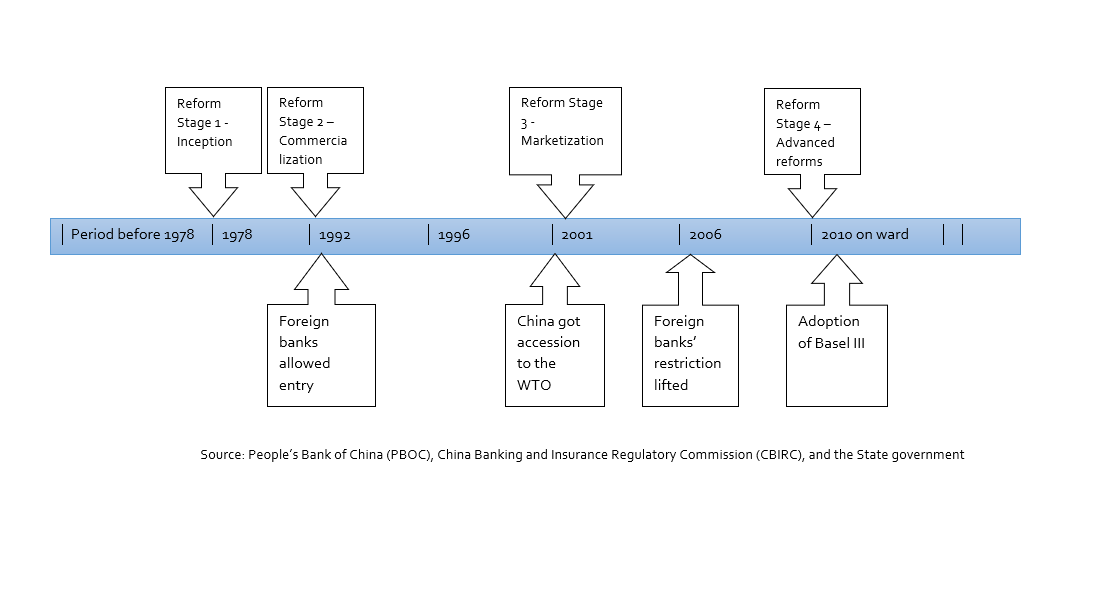
\includegraphics{chapter00-landscape-timeline.png}

}

\caption{\label{fig-timeline}The Financial Reform Timeline}

\end{figure}%

\subsection{The era from 1978 - early
1990s}\label{the-era-from-1978---early-1990s}

China's central bank, the People's Bank of China (PBOC)\footnote{For
  detailed history of the People's Bank of China, see the official
  webpage of the PBOC
  \url{http://www.pbc.gov.cn/en/3688066/3688089/index.html}} was founded
in 1948 with the merging of the North China Bank, Beihai Bank, and the
Northwest Peasant Bank. In 1949, the Chinese People's Political
Consultative Conference designated the PBOC as the central bank and its
national financial functions. The responsibilities of the PBOC included:
issuing and circulating the unified currency -- the Renminbi (RMB),
controlling inflation, managing exchange rates, and centralizing,
allocating, as well as utilizing credit endowment to support and
accelerate national economic recovery.

Before 1978, China's banking system took the form of the `mono-bank'
structure, the idea referencing the financial system of the former
Soviet Union. (Berger et al., 2009) The reason behind this choice relies
upon the fragile social and economic environment China was facing at
that time. After World War II and the civil war, China's economy was
extremely weakened and the social situation was rather severe, with high
level of poverty, unemployment, and inflation. Under these
circumstances, the PBOC established a rudimentary banking system, aiming
at building up people's faith to the government and to their
communities, as well as boosting the national recovery in all aspects.

From 1979, national strategies have shifted to developing and
strengthening the economy from economic recovery. A series of relative
national strategies created and executed by the Chinese government are
usually labeled `Reform-Open' strategies. The essence of the
`Reform-Open' strategies involve: 1) lifting the restriction of
accession to China's domestic markets; 2) loosening the constraints of
foreign shareholding; 3) establishing and fortifying legislation upon
markets, competition, corporate governance, and intellectual property
protection. The reform of financial system is a critical part in the
chain of China's industrial reforms.

During the period between 1979 and 1992, China's banking sector
reconstructed its institutional framework. First, the commercial-banking
function of the People's Bank of China was delegated to four state-owned
commercial banks: Bank of China, China Construction Bank, Agricultural
Bank of China, and Industrial and Commercial Bank of China. These four
commercial banks are traditionally called `the Big Four'. By the time
they were founded or resumed\footnote{Bank of Communications}, their
business was limited in a specified sector of economy, namely foreign
trade, construction, agriculture, and industrial and commercial sectors
(see Berger et al., 2009; Jiang et al., 2009). Second, national banks
came into existence from 1986 (Hsiao et al., 2015). The first national
bank is Bank of Communications which was resumed in 1987 \footnote{Bank
  of Communications was founded in 1908 during the Qing Dynasty. The
  bank was dismantled and its business was taken over by the Big Four
  after 1949. In 1987, Bank of Communication was resumed and performed
  banking business again.}. Apart from the biggest shareholder- the
Finance Ministry, state-owned enterprises were allowed to invest in
banks for the first time. Third, other types of financial institutions
were set up or resumed to complete the financial system. For instance,
the State Administration of Foreign Exchange (SAFE) was founded as the
authority administrating foreign Exchange issues. The People's Insurance
company was re-established.\footnote{The People's Insurance Company was
  existed before 1949. Therefore, the company was re-established in the
  early 1990's.} Trust companies and urban credit cooperatives, as new
players, entered China's financial system. Foreign banks were allowed to
enter China's financial market by operating in Special Economic
Zones\footnote{Special Economic Zones: a form of Free Ports in China
  where companies may benefit from tariff allowances and exemption.
  Chinese government designated the first four Special Economic Zones --
  Shenzhen, Xiamen, Shantou, and Hainan Province -- in order to
  encourage foreign investments and improve economy and technology by
  the end of 1980's. More details may be found in
  \url{http://www.npc.gov.cn/npc/c12434/c234/201905/t20190522_64495.html}}
(Berger et al., 2009). Lastly, starting from 1984, the PBOC performs
solely as a central bank, a decision made by the State Council the
previous year.

A key feature of China's financial reform during this period is the
restructuring at the institutional level, marking the first wave of
China's financial reform. At this stage, new types of players began to
operate in China's financial markets. However, the government still
controlled the ownership of all layers of financial institutions. In
addition to the Big Four banks, city credit cooperatives that emerged
during this period remained wholly owned by local Bureaus of Finance.
This ownership structure persisted because the capital used to establish
these financial institutions originated from the Treasury system(funded
by taxpayers). This initial phase of financial reorganization serves as
a significant milestone in China's reform process. Opportunities for
further changes and development were provided at this stage,
nevertheless, Chinese government exhibited a conservative stance
regarding the entry of foreign banks.

\subsection{Early 1990s - End 2001}\label{early-1990s---end-2001}

Besides financial reforms, industrial reforms took place during the same
period. The first wave of China's industrial reform, which occurred
concurrently with the financial changes, not only granted the
state-owned enterprises greater autonomy in decision-making but also
introduced the `Contract Responsibility System' (CRS) in a tentative
attempt in separation of ownership and management (Lin et al., 2020).
The CRS resembles corporate governance structures in advanced nations.
However, the CRS, functioning within the framework of state-owned
ownership, had certain constraints and led to both positive and negative
outcomes. The CRS boosted the incentives of management of the
state-owned enterprises and at the same time caused some issues such as
superfluous supply and moral hazard problems due to the leeway of the
CRS system.

One of the results was the severe deterioration of loan quality of the
Big Four, since they played a main role in the state-owned enterprises'
financing which were involved directly with the government before
1990's. Concerning the Big Four, several initiatives were adopted. In
1994, three policy banks (China Development Bank, Agricultural
Development Bank of China, Export-Import Bank of China) were established
to undertake the policy-lending function performed by the Big Four. In
1998, Ministry of Finance issued 270 billion RMB of long-term special
Treasury bonds as the supplement capital invested into the Big Four. In
1999, four state-owned asset management companies (AMCs) were founded
and bought in total 1.4 trillion RMB of Non-performing Loans from the
Big Four\footnote{Four state-owned asset management companies: China
  Huarong Asset Management Co., Ltd., China Great Wall Asset Management
  Co., Ltd., China Cinda Asset Management Co., Ltd., and China Orient
  Asset Management Co., Ltd.~}.

Regulatory legislation surrounding financial reforms made a breakthrough
during this period. In 1995, Central Bank Law (the People's Bank of
China Law of the People's Republic of China) and Commercial Bank Law
(Commercial Bank Law of the People's Republic of China) were enacted by
the National People's Congress. Central Bank Law authorizes the People's
Bank of China as the central banks of China to perform regulation and
supervision over China's financial system. Commercial Bank Law clarifies
banks should conduct their business as commercial entities. Commercial
Bank Law also, for the first time, stipulates the requirement of the
capital adequacy towards commercial banks. It requires that commercial
banks must remain the capital adequacy ratios over 8\%.

National banks\footnote{National banks: commercial banks which have
  nationwide branches with no geographical constrains.} transitioned to
a joint-stock ownership structure \footnote{Joint-Stock banks:
  commercial banks which shares are held by institutional investors,
  mainly local treasury bureaus and other enterprises.}. In 1996, China
Minsheng Bank was established and jointly owned by private companies
instead of having state-owned institutions and/or Ministry of Finance as
its shareholders. Required by the State Council, and abiding the
guidance document `State Council Decisions on Financial System Reform'
issued in 1993, urban credit cooperatives located in cities embarked on
merge and consolidation to establish the new type of joint-stock
financial institutions known as city banks. In principle, there would be
one city bank located in one city and provide financial services
focusing on that geographic area. Like city banks, the establishment of
rural commercial banks was also started out on the basis of the
associations of rural credit cooperatives which take private
company-individual shareholding structure. Rural commercial banks
primarily focus their business in rural areas surrounding a city.

The year 1994 marked a significant shift with the `Regulation of the
People's Republic of China governing foreign financial institutions,'
allowing foreign banks to enter China's financial markets. Subsequently,
in 1996, foreign banks were licensed to conduct business in the local
currency in Shanghai Pudong\footnote{Shanghai Pudong District: an area
  similar to the Special Trade Zones where foreign companies have tariff
  and other benefits; officially designated as China (Shanghai) Pilot
  Free Trade Zone in 2013.} and further expanded to neighboring areas
(Berger et al., 2009; Hsiao et al., 2015). Since 1998, foreign banks
have been authorized entry to China's inter-bank market.

A distinguishing feature of the financial reforms during this period is
commercialization of banks. They evolved into genuine commercial
entities, departing from their previous role as `policy-lending
`conduit' (Berger et al., 2009). The 1995 Commercial Bank Law had a
profound impact upon banking industry in the aftermath of its
introduction. During this period, shareholders of banks diversified
compared to the direct government shareholders and the state-owned
shareholders in the first stage of the financial reforms. Alongside with
the government (Ministry of Finance), state-owned enterprises, private
companies even individuals were allowed to invest in banking industry.
The act of embracing foreign financial institutions also improved the
speed of Chinese banks' commercialization, to some extent, regarding
learning from the advanced countries. This period, from the perspective
of ownership structures, marked the beginning of reduced direct
government intervention in banks' operations, owing to the inclusion of
diversified shareholders.

\subsection{WTO accession 2001 - 2010}\label{wto-accession-2001---2010}

China gained entry into the WTO in 2001. The WTO agreement deepened and
broadened China's overall economic reform in terms of the extent and
fields covered. China committed to put much more effort into
legislation, commercial banks' transformation, opening domestic
financial markets to foreign banks, among others. China was granted by
the WTO a five-year transition period to fulfill the commitment in
stages.

Since 2003, several laws have been changed and new institutions have
been founded to align with the WTO agreement and the environment of the
ongoing reforms. The 1995 Central Bank Law was amended to reinforce the
People's Bank of China as the central bank performing monetary policies
and macro-prudential administration. A new regulatory department --
China Banking Regulatory Commission (CBRC)\footnote{In 2018, the China
  Banking Regulatory Commission (CBRC) consolidated the China Insurance
  Regulatory Commission (CIRC) into a new regulatory authority - The
  China Banking and Insurance Regulatory Commission (CBIRC).} was
established. Most of regulatory duties performed by the People's Bank of
China (PBOC) during the initial stages of the economic recovery and
reform were transferred to the CBRC since the end of 2003. By the time
the CBRC was established, its founding law `the Law of the People's
Republic of China on Banking Supervision' also took effect and empowered
the CBRC as the main regulatory body in banking sector. The 1995
Commercial Bank Law also was amended to satisfy the new market
environment by broadening the business scope of commercial banks and
adding more articles in terms of governance, disclosure, and
supervision. In the end of 2006, the amendment of `Regulation of the
People's Republic of China governing foreign financial institutions' was
executed with the new definitions of foreign financial institutions and
new articles in terms of regulation and supervision.

Since 2003, aiming at Initial Public Offering and becoming
market-oriented institutions, the transformation of the state-owned
banks, i.e.~the Big Four, began. At the end of 2003, Central Huijin
Investment Ltd.~(`Central Huijin') was established by the People's
Republic of China (`the State'). Since then, Central Huijin has been
acting as a shareholding representative of the State in those
state-owned financial firms including banks, insurance companies,
securities firms, and other financial firms.\footnote{For detailed
  information, see Central Huijin website
  \url{http://www.huijin-inv.cn/huijineng/About_Us/index.shtml}} Between
2003 and 2008, Central Huijin injected around 125 billion US dollars in
total as supplement capital into the Big Four. During the same period,
the NPLs were bought by the four asset management companies (AMCs) ar
market prices again. After the aforementioned preparation for listing,
during 2005-2007, three of the Big Four went public on Shanghai Stock
Exchange and Hong Kong Stock Exchange. Other national banks such as Bank
of Communications, China Minsheng Bank and China Merchants Bank had been
listed on the domestic stock market before that time. In 2006, Post
Savings Bank of China was founded by China Post Group. The Big Four,
Bank of Communications and Post Savings Bank of China have become the
six Systemically Important Banks in China, i.e.~the Big Six, since 2019.
The assets of the Big Six account for 40.27\% of the total assets of the
banking sector.\footnote{\textless http://www.cbirc.gov.cn/cn/view/pages/ItemDetail.html?docId=890465\&itemId=954\&generaltype=0
  \textgreater{}}

The reforms in city credit cooperatives took further steps following the
WTO agreement. City/urban credit cooperatives\footnote{See regulatory
  document
  \url{http://www.pbc.gov.cn/bangongting/135485/135495/135499/2833472/index.html}}
are a primary financial institutional form in cities during the 1990s,
apart from the Big Four and the national banks. The ownership structure
of city/urban credit cooperatives is joint-investment, the legitimate
shareholders include individual investors and private companies. The
cooperatives mainly provide financial services to the members. In 2005,
the CBRC issued `guidance on development of city credit cooperatives',
proposing that city credit cooperatives should be transformed into
joint-stock banks within three years. In 2006, city commercial banks
were permitted to set up branches and operate in regions other than the
host cities. By the end of 2006, there were 113 city commercial banks
and 78 city credit cooperatives in China. The numbers of city commercial
banks increased to 143 by the end of 2009. In 2007, three city banks
Nanjing Bank, Ningbo Bank and Beijing Bank went public and listed in
Shanghai or Shenzhen Stock Exchange.

Similar to city credit cooperatives, rural credit cooperatives provide
financial services to their members in rural areas. Their primary
shareholders are rural private investors. The reform in rural credit
cooperatives, i.e.~the establishment of rural commercial banks, has also
increased up since 2003. In 2003, the CBRC issued the regulatory
documents `Transitional Regulation on the Administration of Rural
Commercial Banks' and `Transitional Regulation on the Administration of
Rural Cooperative Banks' aiming at regulating those new rural
commercial/cooperative banks\footnote{A rural cooperative bank is a
  transitional structure of a rural financial institution which are
  smaller than a rural commercial bank in size and has the similar
  membership feature as a rural credit cooperative.}. In 2004, the State
Council also issued a policy document seeking to accelerate the reform.
By the end of 2009, there were already 43 rural commercial banks and 196
rural cooperative banks in China's banking sector.

China fulfilled WTO commitments by allowing foreign institutions to
conduct business in its financial markets and permitting them to hold
shares of Chinese banks as strategic investors. The taxonomy `Strategic
Investors' is firstly used by the China Securities Regulatory Commission
(CSRC), referring to those institutional investors which invest in
listed companies for long-term/strategic purposes rather than short-term
financial returns. In the banking sector, strategic investors are mostly
those foreign large financial conglomerates (including foreign banks and
non-banking institutions) which invest in Chinese commercial banks. A
single foreign strategic investor is allowed to hold no more than 20\%
of shares of a Chinese bank; and multiple foreign strategic investors
are allowed to hold in total no more than 25\% of shares of a Chinese
bank.

In 2006, the amendment of `Regulation of the People's Republic of China
governing foreign financial institutions' was issued and took effect.
The restrictions over business region and clientele have been relaxed.
By the end of 2006, there were 312 foreign banking entities\footnote{Foreign
  banking entities entail foreign bank branches, foreign bank
  subsidiaries and foreign joint-stock banks.} conducting business in
China's financial markets, compared to only 192 foreign financial
entities in 2003. During this period, foreign banks also actively
investing in Chinese banks as strategic investors. By the end of 2006,
foreign banks and institutional investors were holding investments in
three of the Big Four, Bank of Communications and several national
banks. The Royal Bank of Scotland Group (RBS Group), Temasek Holdings
Private Ltd., and UBS Group AG totally held 16.85\% of the listed shares
of Bank of China. The Goldman Sachs Group Inc., Allianz Group, and
American Express held 10\% of the listed shares of Industrial and
Commercial Bank of China. Bank of America and Temasek Holdings Private
Ltd.~(also through Asia Financial Holding Group and other subsidiaries)
held almost 20\% of the listed shares of China Construction Bank. HSBC
Group held 19.9\% of the listed shares of Bank of
Communications.\footnote{The data come from the individual banks' annual
  financial reports.} Apart from investing in the state-owned banks and
national banks, foreign financial institutions, as strategic investors,
also invested in city banks such as Xi'an Bank, Nanjing Bank, Ningbo
Bank, Beijing Bank, etc. The period of 2005-2006 is the heyday of
foreign investment into domestic banks, expanding from the biggest
cities such as Beijing and Shanghai, to the medium sized cities such as
Nanjing. By the end of 2006, the amount of foreign investment in Chinese
banks was around 19 billion US dollars, accounting for 0.3\% of the
total assets of the whole banking sector, and 14\% of the total assets
of the foreign banks in China.\footnote{The data come from the CBIRC
  annual report in 2006 and manual computation.}

In terms of banking regulation, on the basis of the adoption of Basel
I\footnote{See \emph{appendix} Table~\ref{tbl-regulatorydocs} for
  detailed information} (1995 Commercial Bank Law stipulated the capital
adequacy). and the incorporation of Basel II, the CBRC issued the
regulation of `Measures of the Capital Adequacy Ratio of Commercial
Banks' in 2004 and its amendment in 2006. This regulation can be
regarded as the China version of Basel II.

Corresponding to the rapid transformation of commercial banks and aiming
at corporate risk management, the CBRC issued a regulatory document
`Regulatory Guidelines of Corporate Governance in State-owned Commercial
Banks' in 2006.

Marketization was a distinctive feature of this reform period. This
period is a crucial stage of China's financial reform during which
almost all influential events and policies concerning regulation and
supervision, ownership structures, corporate governance, among others,
happened.

With regard to ownership structure, the establishment of Central Huijin
is one of the crucial milestones in China's reform of state-owned
financial enterprises. Since the end of 2003, Central Huijin, as a
shareholder, has gradually replaced the direct role of the State
government in those state-owned financial firms. Central Huijin acts as
a representative of the State government which is the shareholder of the
state-owned firms. The momentum of this fundamental change could stem
from China's commitment to the WTO and the upcoming pressure of the
competition with foreign financial firms. In 2007, the founding of
China's sovereign wealth fund -- China Investment Corporation (CIC) took
the abovementioned reform a step forward. Central Huijin became a
wholly-controlled subsidiary of CIC. The establishment of Central Huijin
played a crucial role in reforming state-owned financial enterprises,
representing a shift from direct government intervention to indirect
control through shareholding.

Getting listed is also an imperative strategy in China's financial
reforms. It dramatically enriches the shareholder profiles: transforming
government shareholding, accepting private enterprises, embracing
foreign investors, and partially privatizing (individual investors).
More importantly, it promotes the establishment of modern corporate
governance frameworks in banks, both listed and non-listed; which
reciprocally validates and strengthen the reform. It was in this period
that multiple categories of banks' ownership structure rose and became
the foundation and the consensus in the future development of China's
banking sector.

\subsection{2010 onward}\label{onward}

The literature does not, generally, define the time since 2010 as part
of the `reform period'. This may be because: 1) during 1990s and 2009,
substantial and fundamental reforms were successfully performed and the
infrastructure of financial industry in terms of legislation,
regulation, and corporate governance were founded; 2) 2007-2008 the
worldwide financial crisis drastically changed the landscape of the
financial industry; 3) reforms implemented after 2010 are usually
considered as improvements or advanced changes on the basis of the
achievements of the previous reforms. Nonetheless, there are still
important changes in China's banking sector during this period.

Since 2009, further changes concerning the corporate governance
framework were implemented in state-owned banks including policy banks
and state-owned commercial banks. Notably, in 2010, Agricultural Bank of
China listed on both Shanghai Stock Exchange and Hong Kong Stock
Exchange. After the introduction of 10 foreign and domestic strategic
investors including UBS Group AG, JP Morgan Chase, Temasek Holdings
Private Ltd., China Life Insurance Group, and etc. in 2015, Post Savings
Bank of China finished its Initial Public Offering (IPO) on Hong Kong
Stock Exchange in 2016, and also listed on Shanghai Stock Exchange at
the end of 2019.

From 2010 onward, comprehensive reforms targeted city banks, or more
generally, small-middle sized banks, focusing on ownership structures
and target markets. Regulatory measures were introduced to diversify
ownership profiles. In 2010, the CBRC issued the regulatory document
`Notice on the Examination of Qualification of Major Shareholders of
Small and Medium-sized Commercial Banks' to restrain the share of a
single major shareholder (the shareholder which have controlling shares
or voting rights) within 20\% of the shares of a small and medium-sized
commercial bank. This regulatory document aims at constructing city
banks as the financial institutions jointly owned by shareholders with a
diversified ownership profile. In 2019, the China Banking and Insurance
Regulatory Commission (CBIRC) issued a regulatory document `Measures of
License Issues in Rural Small and Medium-sized Banking institutions',
stipulating that non-financial institutions and their related parties as
shareholders are not allowed to hold more than 10\% of the total shares
of a rural commercial bank. Since 2013, private enterprises have been
permitted to invest in small and medium-sized commercial banks as
founding shareholders. In 2014, 5 private joint-stock commercial banks
were founded.\footnote{Five private joint-stock commercial banks:
  Kincheng Bank of Tianjin Co., Ltd., Shanghai Huarui Bank Co., Ltd.,
  Zhejiang E-Commerce Bank Co., Ltd., Myshare Bank of Wenzhou Co., Ltd.,
  Shenzhen Qianhai WeBank Co., Ltd.} By 2017, private institutional
shareholding accounted for 43\% in national banks, 55\% in city banks,
and 87\% in rural financial institutions. In 2016, 7 city banks got
listed in Shanghai or Shenzhen Stock Exchange, and 8 city banks finished
their IPO in Hong Kong Stock Exchange. By the end of 2019, there a total
of 20 city banks listed. Regarding the target market, in 2011, the CBRC
issued guidance documents to encourage small and medium-sized banks to
target small and micro enterprises\footnote{According to `the Law of the
  People's Republic of China on the Promotion of Small and Medium
  Enterprises', small and medium enterprises should submit application
  to the government to define whether they are small and medium
  enterprises. Generally, enterprises which have revenue under USD70,000
  (RMB 500,000 Yuan) can be defined as micro enterprises. Enterprises
  which have revenue between USD70,000 - USD700,000 can be defined as
  Small enterprises.} as their clientele.

Qualified rural credit cooperatives have continued to be transformed
into rural commercial banks and the modern corporate governance
framework was established as early as 2010. Those unqualified were
designated as town-village banks or credit cooperatives as supplemental
financial organizations to serve their local rural community. By the end
of 2017, there have been in total 1351 rural commercial banks. As an
example of the success in the ownership structure reforms, Chongqing
Rural Bank completed its IPO in the Hong Kong Stock Exchange in 2010.
There were 10 listed rural commercial banks by the end of 2019.

Foreign banking entities continue to increase by volume and by total
assets year on year since 2009, given that the Chinese government took
the opening-strategy a step further. In 2014, the State Council issued
the amendment of the 2006 `Regulation of the People's Republic of China
governing foreign financial institutions',\footnote{The 2006 `Regulation
  of the People's Republic of China governing foreign financial
  institutions' itself was an amended version of the original 1994
  'Regulation of the People's Republic of China governing foreign
  financial institutions.} lifting more restrictions regarding founding
and operating foreign banking entities in China's domestic financial
markets. Since 2009, new foreign banking entities began emerging in the
north-east and the central-west provinces and medium-to-small sized
cities where the economy is rather under-developed. By the end of 2016,
1031 foreign banking entities have been founded and are operating in
over 70 cities in 27 provinces (including the province-level
municipalities).

A parallel strategy to opening financial markets and embracing foreign
companies is known as `going-abroad' strategy. Those qualified
commercial banks and policy banks have started to go abroad and set up
branches and/or subsidiaries in foreign countries after they established
the corporate governance frameworks and control systems. By 2017, 23
banks (commercial banks and policy banks) have set up 238
subsidiaries/branches/representatives in 65 foreign countries (regions).

Aligning with the Basel III framework, the CBRC issued `Commercial Bank
Capital Management Measures', -- the China version of Basel III in 2012.
China's regulatory authorities fully adopted Basel III \footnote{See
  appendix Table~\ref{tbl-regulatorydocs} for detailed information},
incorporating it into the domestic regulations and setting up the
transition period matching the requirement of Basel Committee. Targeting
regulatory arbitrage and shadow banking, the CBRC issued regulatory
documents to rule and rectify the thriving wealth management products
and inter-bank market in 2014 and 2015. Also as a complement to
corporate governance guidance, the regulatory document `Guidelines of
Administration and Supervision on Consolidation of Commercial Banks'
requires commercial banks to consolidate domestic and foreign
subsidiaries and conduct comprehensive risk management.

More nuanced improvements and adjustments have also taken place since
2010 based on the implementation in previous stages. The ownership
structure evolved, with diversified models becoming mainstream including
state-owned, joint-stock with local government holding, joint-stock with
private company shareholders in China's financial institutions. Among
others, establishment of a modern corporate governance framework is
considered as a safeguard against direct government interference in
banks' decision-making; although the evidence of the recedes of direct
government in practice need to be investigated further. The last forty
years' reform substantially changed the role that the State government
and local government played in the economy: from directly designing
economic development plans and managing enterprises to fostering a
conducive market environment for competition and upholding macroeconomic
stability (Atherton and Newman, 2016).

One of the most salient reforms in banking regulation is the issuance of
`Commercial Bank Capital Management Measures' -- the China version of
Basel III by the CBRC in 2012. It not only changes the way of China's
regulatory authorities regulating and supervising banks, but also
requires commercial banks to be accountable for their business
decisions. To some extent, this new regulation also can be viewed as the
withdrawal of implicit government resort as presented in the early years
of the financial reforms.

As part of the significant systemic industrial Reform in China's
economy, the financial reform in the banking sector transformed the
landscape forstering marketization, securitization, and globalization.
The reform and development in legislation and transformation resulted in
diversified ownership structures, modern corporate governance, and
market competition. From the perspective of corporate governance, the
direct government intervenes can be considered receding step by step in
rounds of the reform. The further deepening overhaul, taking the global
financial crisis as an opportunity, is taking place in a fast pace and
contributes to the further growth of China's financial system.

\section{Part II: the Chinese banking regulatory
framework}\label{part-ii-the-chinese-banking-regulatory-framework}

Along with the overall banking sector reforms, the banking regulatory
framework has also experienced considerable changes. In this section, we
will briefly review the evolution of the banking regulatory framework,
then introduce the main factors of the framework as follows: the
regulatory authorities, the regulated institutions, and the regulated
fields.

\subsection{Historical overview of the Chinese banking
regulators}\label{historical-overview-of-the-chinese-banking-regulators}

We begin with a brief history of the evolution of banking regulators in
China.

Until 1978, the Chinese banking system was following the mono-bank
model. The only bank, - the People's Bank of China (PBOC), which acted
as a unit of the State Council and was appointed as `a National Bank',
undertook functions including `issuing national currency, managing
national treasury, managing national finance, stabilizing financial
markets and supporting economic recovery'\footnote{See the website of
  the People's Bank of China
  \url{http://www.pbc.gov.cn/rmyh/105226/105433/index.html}} following
its establishment. Following the incorporation of private financial
institutions into the financial system, the PBOC played a dual role in
the financial system: a central bank as well as a commercial bank. The
PBOC performed its supervisory function through directly controlling
permission for the establishment of financial institutions, approval of
their key operational decisions, and senior management appointments in
financial institutions.

The national economic reform began in 1979, which necessitated the
function transformation of the PBOC and establishment of a diverse
financial system. Since 1984, the PBOC performs solely as a central
bank, which was decided by the State Council the year before. In 1995,
`the People's Bank of China Law of the People's Republic of China'
reinforced the PBOC's status as a central bank through legislation.

In 2003 the regulatory function was officially separated from the PBOC
and transferred to the newly founded supervisory body, - the China
Banking Regulatory Commission (CBRC). Since then, the CBRC has been
regulating banks and financial institutions other than insurance
companies and securities firms. In 2018, the CBRC was merged with the
China Insurance Regulatory Commission into a new regulatory body, - the
China Banking and Insurance Regulatory Commission (CBIRC) which is
responsible for regulating banking and insurance sectors.\footnote{See
  the official document of the Chinese Government `The Central Committee
  of the Communist Party of China issued the `Deepening Party and State
  Institution Reform Plan'
  \url{http://www.gov.cn/zhengce/2018-03/21/content_5276191.htm\#2}.}

\subsection{The current main regulators in banking regulation and
supervision}\label{the-current-main-regulators-in-banking-regulation-and-supervision}

Authorized by its founding laws, the China Banking and Insurance
Regulatory Commission (CBIRC) and the People's Bank of China (PBOC) are
the two main regulators in bank regulation and supervision in China.
These two regulators have the authority to issue regulatory documents in
forms of rules, decrees, notices, etc. to regulate and oversee financial
institutions. A chart of the structure of the framework of regulation
and supervision in China can be found in Figure~\ref{fig-regulators}.

\begin{figure}

\centering{

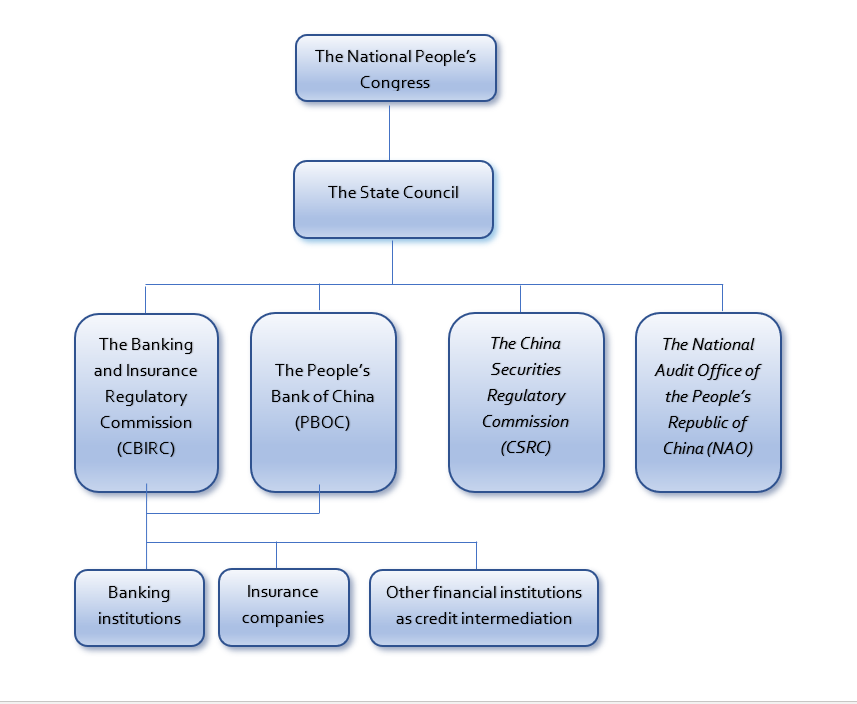
\includegraphics{chapter00-landscape-regulators.png}

}

\caption{\label{fig-regulators}The Structure of The Banking Regulatory
and Supervisory Framework in China}

\end{figure}%

\subsubsection{The China Banking and Insurance Regulatory Commission
(CBIRC)}\label{the-china-banking-and-insurance-regulatory-commission-cbirc}

The China Banking and Insurance Regulatory Commission (CBIRC) was
established in 2018 combining two previously separated regulatory
commissions, -- the China Banking Regulatory Commission (CBRC) and the
China Insurance Regulatory Commission (CIRC). The motivation behind
combining these two regulatory commissions is that there were
supervision gaps between banking and insurance sectors as well as the
imbalance of supervisory resource. The aims of the merger are to
eliminate the supervisory gaps and to clarify the supervisory
responsibilities as well as optimizing allocation of supervisory
resource.\footnote{See the official document of the Chinese Government
  `The Central Committee of the Communist Party of China issued the
  `Deepening Party and State Institution Reform Plan'
  \url{http://www.gov.cn/zhengce/2018-03/21/content_5276191.htm\#2}.}

The CBIRC is the major player in the Chinese banking regulatory
framework. Besides the official document issued by the Chinese
Government, the CBIRC is empowered by the Law of the People's Republic
of China on Banking Supervision, the Law of the People's Republic of
China on Commercial Banks, and other relevant laws and administrative
documents such as the Law of the People's Republic of China on the
People's Bank of China and the state government document `China Banking
Insurance Regulatory Commission's functional configuration, internal
institutions and staffing regulations'.

The mandates listed in the above central document and its official
website of the CBIRC include:

\begin{enumerate}
\def\labelenumi{\Roman{enumi})}
\tightlist
\item
  Rule-making and enforcement
\end{enumerate}

The CBIRC is authorized by the People's Congress to issue two types of
regulatory rules: regulations and regulatory documents.\footnote{According
  to CBIRC, the regulations have more powerful authority than regulatory
  documents.} Most of these rules are issued in the forms of Notices or
Decrees by the CBIRC. The regulatory rules are legally bound and the
breaches would be subject to the commensurate legal punishment according
to the legal force of the regulations or the regulatory documents.

\begin{enumerate}
\def\labelenumi{\Roman{enumi})}
\setcounter{enumi}{1}
\tightlist
\item
  Oversight and supervision
\end{enumerate}

The CBIRC ensures that the regulatory rules are adhered through their
oversight and supervision on financial institutions' behavior and
disclosure. The CBIRC may conduct on-site inspection and compliance
assessments as well as supervise banks (and insurance companies) on
corporate governance, risk management and internal control. The CBIRC
also establishes risk monitoring and evaluation systems on banks (and
insurance companies) in terms of capital adequacy, solvency and other
stability and soundness requirements.

\begin{enumerate}
\def\labelenumi{\Roman{enumi})}
\setcounter{enumi}{2}
\tightlist
\item
  Licensing, chartering, and registration
\end{enumerate}

The CBIRC issues licenses and charters to banks (and insurance
companies) in terms of the access to financial markets and the business
scopes. It also has the authority to influence the appointment of senior
management in the regulated financial institutions.

The banking regulatory framework in China is a `CBIRC centric'
framework. The CBIRC has established its dispatched agencies and
affiliates in all provinces and eight key cities such as Beijing,
Shanghai, and Shenzhen on the mainland. These affiliates in different
regions are called `Supervision Bureaus' which directly report to the
CBIRC headquarter. This two-tier structure facilitates the effective
execution of regulations and supervision.

\subsubsection{The central bank -- the People's Bank of China
(PBOC)}\label{the-central-bank-the-peoples-bank-of-china-pboc}

Most of regulatory duties performed by the People's Bank of China (PBOC)
during the initial stages of the economic recovery and reform has been
transferred to the CBRC since 2003. The legal status of the PBOC as the
central bank of the People's Republic of China was established by the
Law of the People's Republic of China on the People's Bank of China in
2003. As the central bank, the PBOC conducts monetary policies,
targeting short-term interest rates through open market
operations.\footnote{Open market operations refer to the PBOC buys and
  sell Treasury Bonds on the open market in order to control the money
  supply.} The PBOC also may provide loans to commercial banks, acting
as a `lender of last resort'.

The PBOC is still closely tied to the stability and soundness of the
financial system in China. The regulatory functions of the PBOC focus on
regulating bank behavior in interbank markets involving repurchase
agreements (Repo), interbank foreign exchanges, and interbank bonds. The
PBOC also issues regulatory rules on the payment system cooperating with
the CBIRC.

China takes the form of the dual-regulator architecture on banking
supervision. The PBOC acts as the monetary authority of China, and
performs supervisory responsibility on payment systems. The CBIRC acts
as the primary regulatory authority of the banking sector. The adoption
of a single regulator has been a common feature of banking during the
last three decades (Herring and Carmassi, 2008). For example, the
European Central Bank has direct supervisory responsibilities over banks
in the Eurozone and the Federal Reserve in the United States
strengthened its supervisory power by Dodd-Frank Act. The advantages of
the single regulator structure include economies of scale and scope,
reduction of potential regulatory arbitrage, the ability to supervise
the complicated financial conglomerates, among others (Doumpos et al.,
2015). Internationally, the Reserve Bank of Australia and the Bank of
Japan do not perform the direct supervision over the domestic banking
sectors (Berger et al., 2017). China takes the dual-regulator
architecture which might avoid the disadvantages of the single-regulator
structure, such as potential conflict within a single regulator, the
monopoly power and the moral hazard issues, as reported in (Doumpos et
al., 2015).

\subsection{Other relevant regulators}\label{other-relevant-regulators}

Chinese banks are also subject to regulators other than the two
aforementioned major players. These regulators, as components of the
whole regulatory framework, have specific regulatory functions and
regulatory objectives. The following regulators involved in banking
regulation and supervision usually do not issue specific regulatory
documents targeting financial institutions; rather, financial
institutions are required to comply with the regulation issued by these
regulators. Therefore, the duties of the following regulators complement
the regulation and supervision performed by the two major regulators.

\textbf{\emph{The China Securities Regulatory Commission (CSRC)}} was
founded to regulate the areas over the following: (i) participants in
securities markets; (ii) securities markets; and (iii) securities
products. The CSRC is primarily concerned with transparency and fairness
of the securities markets and investor protection. According to the
CSRC, by the end of 2019 there were 37 banking firms\footnote{See
  `Industry classification results of listed companies in the fourth
  quarter of 2019' by the CSRC
  \url{http://www.csrc.gov.cn/csrc/c100103/c1451996/content.shtml}.}
publicly traded in the domestic market and they are subject to
supervision by the CSRC in terms of financial information disclosures,
securities issuance, and other publicly trading information.

Unlike banking regulators, the CSRC does not have regulatory force
directly on banking firms and may not be able to intervene or prevent
banks from taking excessive risks. However, under the supervision of the
CSRC, listed banking firms are required to truthfully and thoroughly
disclose their financial information which may indicate potential risks
to investors. Banks that intend to list in the near future must submit
their financial and internal control reports to the CSRC.

\textbf{\emph{The National Audit Office of the People's Republic of
China (NAO)}} is a department of the State Council and has the
authorized duty to audit the firms controlled or dominated by the
State-owned capital.\footnote{See the website of the National Audit
  Office of the People's Republic of China
  \url{https://www.audit.gov.cn/en/n744/index.html}.} Differing from
banking firms in most advanced countries, the five biggest banks in
China are controlled or dominated by either Central Huijin Investment
Co., Ltd or directly by the Ministry of Finance of the People's Republic
of China. These State-owned banks are also under the supervision of the
NAO in terms of financial information and corporate governance. Similar
to the CSRC, bank stability and soundness might be an indirect concern
of the NAO over banking firms. As an auditor recruited by the State
government, the NAO mainly concerns about the truthful disclosure of the
employment of the state capital and there are no illegal activities that
may harm the state capital in banks. However, banks are bound by the
regular reports and inspections by the NAO and need to present their
safety and soundness.

\subsection{Regulated financial institutions and regulated
businesses}\label{regulated-financial-institutions-and-regulated-businesses}

According to its founding laws, the CBRC has the authority to regulate
and supervise all institutions in the financial sector including
`commercial banks, urban credit cooperatives, rural credit cooperatives
and other financial institutions and policy banks that absorb public
deposits'. Besides these depository institutions, the CBRC extends its
regulatory authority to asset management companies, trust and investment
companies, internal financial intermediaries in corporations, financial
lease companies, and other financial institutions permitted by law.
These financial institutions are also legally bound by the Law of the
People's Republic of China on Banking Supervision. After the combination
of the CBRC and the CIRC, the regulatory authority of the CBIRC extends
to all insurance companies including insurance brokers.

Foreign banks (including Chinese-foreign joint-stock banks) are also
subject to the regulation and supervision of the authorized regulators
such as the CBIRC and the People's Bank of China. The `Regulation of the
People's Republic of China on the Administration of Foreign Banks',
which has the highest legal force on foreign banks' operating in
financial markets in China, was issued in 2008 as a decree of the State
Council and has been revised twice since then.\footnote{See the website
  of the central government,
  \url{https://www.gov.cn/zhengce/content/2008-03/28/content_1958.htm}.}
Responding to this legal document, the CBIRC issued `People's Republic
of China Foreign Banks Regulations Implementation Rules' in
2015.\footnote{See the website of the CBIRC
  \url{http://www.cbirc.gov.cn/cn/doc/9103/910303/91030302/020943393088424EBD4670788398111B.html}.}
This implementation document provides more detailed guidance to foreign
banks in all aspects of their operation in China.

It is noticeable that in the 2nd amendment of the `Regulation of the
People's Republic of China on the Administration of Foreign Banks', the
requirements on the regulatory capital adequacy ratio has been
underlined and included into legal articles.

According to the statistics from the CBIRC, by October 2019, the six
largest banks\footnote{The six largest banks, also called the
  State-controlled large commercial banks, include the Industrial and
  Commercial Bank of China, China Construction Bank, Agricultural Bank
  of China, Bank of China, Bank of Communications, and Postal Savings
  Bank of China.} have a combined share of about 47.9\% of the total
assets of commercial banks. Four of these six largest banks (the
Industrial and Commercial Bank of China, China Construction Bank,
Agricultural Bank of China, Bank of China) have been listed as Global
Systemically Important Banks (G-SIBs) by the Financial Stability Broad
(FSB) in 2019.\footnote{See the FSB website
  \url{https://www.fsb.org/2019/11/2019-list-of-global-systemically-important-banks-g-sibs/}.}

There two main areas of banking business are under the oversight of the
CBIRC and the central bank. Apart from the expansion of regular banking
business, the rapid growth of shadow banking has become a new concern
and a key area that attracts regulation and supervision.

\begin{enumerate}
\def\labelenumi{\alph{enumi})}
\tightlist
\item
  Regular banking business
\end{enumerate}

According to the `Law of the People's Republic of China on Banking
Supervision' and the `Commercial Bank Law of the People's Republic of
China', all businesses and products within the business scopes of the
domestic and foreign commercial banks should be either approved by or
filed to the CBIRC and/or the People's Bank of China. The regular
banking business encompasses a broad range of products and transactions
such as absorbing deposits and issuing loans, issuing financial bonds,
interbank lending, buying, and selling bonds, credit/debit card
business, among others.

\begin{enumerate}
\def\labelenumi{\alph{enumi})}
\setcounter{enumi}{1}
\tightlist
\item
  Shadow banking
\end{enumerate}

It is believed that the emergence of a large amount of Wealth Management
Products (WMPs) indicates the rapid rise of shadow banking in China. As
it is shown in Figure~\ref{fig-shadowbanking}, China's other financial
institution (OFI) assets have increased to 11.8 trillion US dollars in
2017, accounting for 10\% of the global OFI asset shares and becoming
the third-largest jurisdiction(FSB, 2019). FSB also reported that the
shares of China's shadow banking have been monotonously increasing from
2011 to 2017 (as shown in the right histogram of
Figure~\ref{fig-shadowbanking}).

\begin{figure}

\centering{

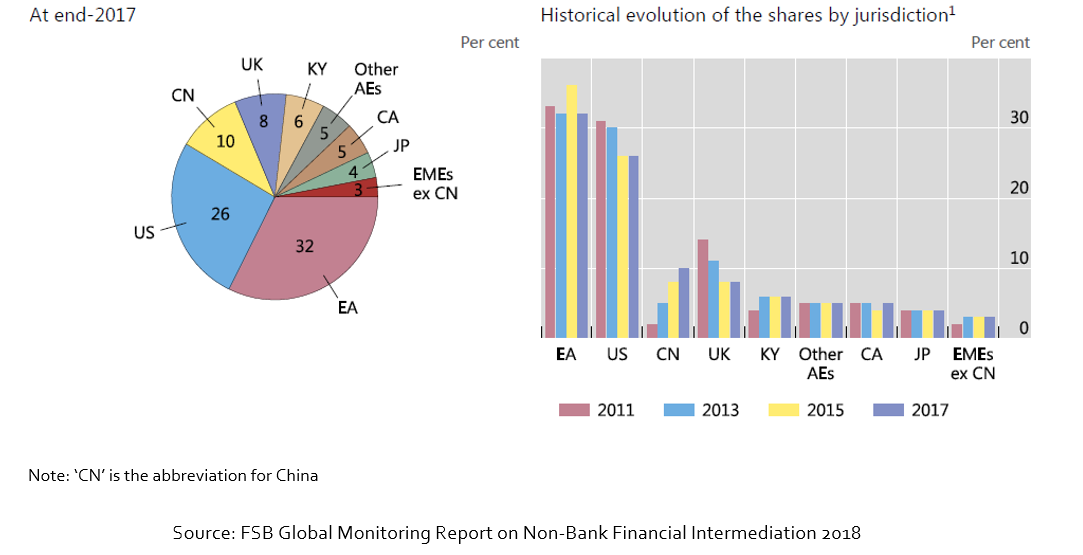
\includegraphics{chapter00-landscape-shadowbanking.png}

}

\caption{\label{fig-shadowbanking}China's Other Financial Institution
Assets Share}

\end{figure}%

Banks dominate the Chinese financial sector. It is understandable that
commercial banks act as the largest and direct intermediaries in shadow
banking in China (Berger et al., 2019). Banks participating in shadow
banking could be considered as a way of regulatory arbitrage. The risks
involved in shadow banking such as liquidity risk, high leverage, and
operational risk might also be imposed on the whole financial system and
the real economy and cause the systematic breakdown. Shadow banking now
has become one of the key areas which needs to be supervised by the
national regulators through stricter regulatory initiatives.

\subsection{Adoption of Basel III framework and rules issued to regulate
the shadow-banking
system}\label{adoption-of-basel-iii-framework-and-rules-issued-to-regulate-the-shadow-banking-system}

As a member of the G20\footnote{G20: An international forum for the
  governments and central bank governors from 19 countries and the
  European Union (EU) in order to promote international cooperation.}
and Basel Committee on Banking Supervision (BCBS, or Basel Committee),
China has been fully supporting and participating in the global
regulatory reform after the Great Financial Crisis\footnote{the
  financial crisis from 2007 to 2009}. In June 2012, the CBRC\footnote{The
  CBRC and the CIRC were combined into the CBIRC in 2018.} issued the
regulation `Commercial Bank Capital Management Measure (Trial)', which
means that the Basel III framework has been adopted and incorporated
into the banking regulatory framework in China.\footnote{China also
  adopted and implemented Basel II and Basel II.5 in previous years.}
The BCBS also assessed the adoption as `compliant' and `largely
compliant' in their assessment report in the Regulatory Consistency
Assessment Program (RCAP) in 2013 (BCBS, 2013).

Following 2012, the CBRC issued or updated supplementary regulatory
documents involving requirements covering all aspects of Basel III
framework to improve the banking regulatory framework in China. Key
regulatory documents can be found in the Appendix
Table~\ref{tbl-regulatorydocs}.

Besides the full adoption of Basel III framework, the Chinese banking
regulatory authorities have noticed the rapid growth of shadow banking
(as shown in Figure~\ref{fig-shadowbanking}). As a member of G20, China
commits to the annual monitoring exercise conducted by the Financial
Stability Board (FSB). The authorities also have started taking
initiatives in order to regulate this particular area to avoid the
damage it could possibly cause. As early as in 2011, the CBRC issued the
regulatory document `Measures for the Administration of Sales of Wealth
Management Products (WMPs) of Commercial Banks', requiring commercial
banks to reveal the risk associated with the WMPs which they are selling
to their customers. Also, in the same year, the CBRC issued a notice
which is linked to a regulatory document targeted at the joint Wealth
Management Products between banks and trusts. In this notice the CBRC
further required that the amount of the WMPs should be reduced
gradually. In 2017, the CBRC announced another notice addressing to
stricter regulation on the WMPs joint business between banks and trusts.

In 2018, the CBIRC issued the regulation `Measures for the Supervision
and Administration of Wealth Management Business of Commercial Banks'
which particularly addresses to commercial banks, the largest and direct
intermediaries in shadow banking. As to those Special Purpose Vehicles
(SPVs) founded by commercial banks to buying and selling WMPs, the CBIRC
issued regulations `Measures for the Management of Wealth Management
Subsidiaries of Commercial Banks' and `Measures for the Management of
Net Capital of Wealth Management Subsidiaries of Commercial Banks' in
2018 and 2019 respectively. These regulations intend to impose more
stringent regulation and supervision on the business line of WMPs.

Under the oversight of the two main regulators -- the CBIRC and the
PBOC, supplemented by other related regulated bodies such as the China
Securities Regulatory Commission (CSRC), the banking regulatory
framework was established and evolved in the past four decades.
Financial institutions involved with banking business, not only banks,
are monitored and supervised under this regulatory framework. The full
adoption of Basel III framework not only symbolizes China's support for
the global regulatory reform, but also represents the further growth of
China's banking sector in terms of regulation and supervision. After the
adoption of Basel III framework, China's two main regulators the CBIRC
and the PBOC have switched their focus to macroprudential supervision,
as instructed by the Bank for International Settlement (BIS). Because of
the rapid growth of shadow banking globally as well as domestically and
its potential influence on the stability of the whole banking system,
shadow banking has become a focusing regulated area in China's banking
sector. As shown in (FSB, 2020), the growth rate and the value of shadow
banking already started to decelerate in terms of total financial
assets, compared to 2019.

\section{Part III: Ratio analysis}\label{part-iii-ratio-analysis}

\subsection{Data}\label{data}

We use the SNL database (a service provided by S\&P Global Inc.) as our
main data source. Our sample is unbalanced. In the analysis of total
assets, our sample entails the data of 5 banking sub-sectors - banks,
insurance companies, securities firms (broker-dealers), trust companies
and specialty lending companies- in total 342 financial institutions
over the period 2010-2019. In the CAMELS system\footnote{The CAMELS
  rating system evaluates a bank's strength across six key categories:
  capital adequacy, assets, management capability, earnings, liquidity,
  and sensitivity. For more detailed information, see Federal Reserve
  website and the Commercial Bank Examination Manual
  \url{https://www.federalreserve.gov/publications/files/cbem.pdf}.}
ratio analysis, we use the data of 231 commercial banks over the period
2010-2019, totaling 2097 observations. In case the SNL database does not
provide enough information or has doubtful values, we hand-collect data
from other official sources including the annual issues of China's
Statistical Yearbook, press releases and the annual reports of the China
Banking and Insurance Regulatory Commission (CBIRC), and the annual
reports of individual banks and other types of financial institutions.
The categories of financial institutions of the banking sector and their
ownership structures can be found in Table~\ref{tbl-allownership}.

\begingroup\fontsize{8}{10}\selectfont

\begin{longtable}[t]{>{}lr}

\caption{\label{tbl-allownership}Ownership structure information of the
banking sector}

\tabularnewline

\toprule
\textbf{Description} & \textbf{Number of Institutions(by 2019)}\\
\midrule
\endfirsthead
\multicolumn{2}{@{}l}{\textit{(continued)}}\\
\toprule
\textbf{Description} & \textbf{Number of Institutions(by 2019)}\\
\midrule
\endhead

\endfoot
\bottomrule
\multicolumn{2}{l}{\rule{0pt}{1em}\textit{Data source:}}\\
\multicolumn{2}{l}{\rule{0pt}{1em}the SNL database, the China Banking and Insurance Regulatory Commission (CBIRC) and manual calculation.}\\
\endlastfoot
\textbf{Total number} & 231\\
\addlinespace[0.3em]
\multicolumn{2}{l}{\textbf{Banks-Border}}\\
\hspace{1em}\textbf{Chinese banks} & 198\\
\hspace{1em}\textbf{Foreign bank subsidiaries} & 33\\
\addlinespace[0.3em]
\multicolumn{2}{l}{\textbf{Public Offering(Chinese Banks)}}\\
\hspace{1em}\textbf{Listed banks} & 50\\
\hspace{1em}\textbf{Non-listed banks} & 148\\
\addlinespace[0.3em]
\multicolumn{2}{l}{\textbf{Place Listed(Chinese Banks)}}\\
\hspace{1em}\textbf{Listed-Mainland} & 36\\
\hspace{1em}\textbf{Listed-Hong Kong} & 15\\
\addlinespace[0.3em]
\multicolumn{2}{l}{\textbf{Bank Ownership}}\\
\hspace{1em}\textbf{State-owned\_Big Six} & 6\\
\hspace{1em}\textbf{State-owned\_Non-BigSix} & 8\\
\hspace{1em}\textbf{Local government-holding} & 58\\
\hspace{1em}\textbf{Joint-stock} & 114\\
\hspace{1em}\textbf{Foreign joint-stock} & 12\\
\hspace{1em}\textbf{Foreign-owned} & \vphantom{1} 33\\
\addlinespace[0.3em]
\multicolumn{2}{l}{\textbf{Bank Type}}\\
\hspace{1em}\textbf{Big Six} & 6\\
\hspace{1em}\textbf{National bank} & 12\\
\hspace{1em}\textbf{City bank} & 110\\
\hspace{1em}\textbf{Rural commercial} & 70\\
\hspace{1em}\textbf{Foreign-owned} & 33\\
\addlinespace[0.3em]
\multicolumn{2}{l}{\textbf{Insurance Companies}}\\
\hspace{1em}\textbf{Total number} & 37\\
\hspace{1em}\textbf{State-owned} & 19\\
\hspace{1em}\textbf{Joint-stock} & 14\\
\hspace{1em}\textbf{Foreign joint-stock} & 4\\
\addlinespace[0.3em]
\multicolumn{2}{l}{\textbf{Securities Firms}}\\
\hspace{1em}\textbf{Total number} & 44\\
\hspace{1em}\textbf{State-owned} & 7\\
\hspace{1em}\textbf{Local government-holding} & 15\\
\hspace{1em}\textbf{Joint-stock} & 20\\
\hspace{1em}\textbf{Foreign joint-stock} & 2\\
\addlinespace[0.3em]
\multicolumn{2}{l}{\textbf{Trust Companies}}\\
\hspace{1em}\textbf{Total number} & 23\\
\hspace{1em}\textbf{State-owned} & 5\\
\hspace{1em}\textbf{Local government-holding} & 7\\
\hspace{1em}\textbf{Joint-stock} & 7\\
\hspace{1em}\textbf{Foreign joint-stock} & 3\\
\hspace{1em}\textbf{Foreign-owned} & 1\\
\addlinespace[0.3em]
\multicolumn{2}{l}{\textbf{Specialty Lending Companies}}\\
\hspace{1em}\textbf{Total number} & 6\\
\hspace{1em}\textbf{State-owned} & 2\\
\hspace{1em}\textbf{Joint-stock} & 4\\*

\end{longtable}

\endgroup{}

\subsection{Total Assets}\label{total-assets}

\begin{figure}

\centering{

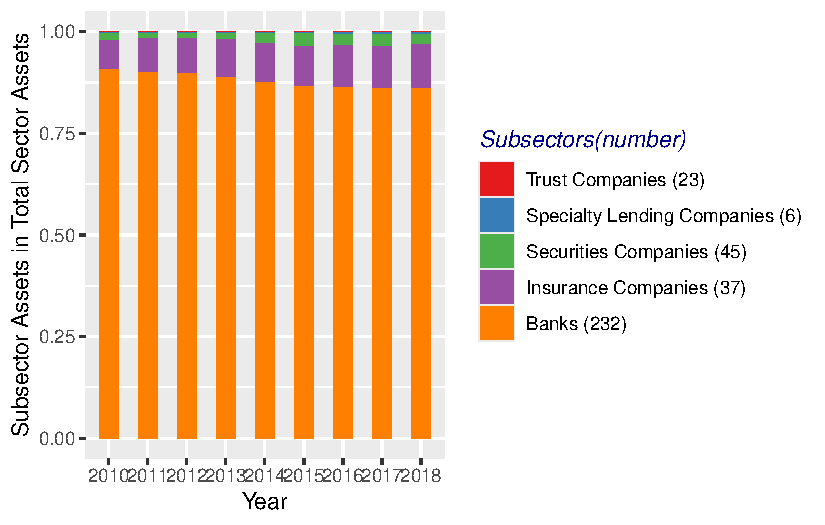
\includegraphics{chapter00-landscape_banking_files/figure-pdf/fig-TotalAssets-1.pdf}

}

\caption{\label{fig-TotalAssets}Banking Sector Assets Total Shares -
Overview(2010-2018)}

\end{figure}%

Figure~\ref{fig-TotalAssets} shows the shares of the total assets of the
subsectors (including banks, insurance companies, securities companies,
trust companies and special lending companies) to the total assets of
banking sector between 2010-2018, based on the categories by the China
Banking and Insurance Regulatory Commission (CBIRC).

The total assets of the whole banking sector (including banking and
non-banking financial institutions) and of the banking institutions have
been increasing between 2010-2019. The total assets of the whole banking
sector amount to RMB 2,825 trillion (approximate USD 403.5 trillion) at
the end of 2019. Figure~\ref{fig-TotalAssets} shows that the banks are
the biggest subsector of the banking sector, in terms of the numbers of
the institutions and their total assets. It also shows that the
proportion of the total assets of the bank subsector have been
decreasing between 2010 to 2018, whereas other subsectors increased. The
reasons that the shares of the banks remained stable or even decreasing
in the recent three or four years could be the rising of the shares of
other financial institutions, including securities firms, insurance
companies, FinTech companies etc., which also are incorporated into the
whole banking sector (see Berger et al., 2019). This trend represents
that more financial services and functions have been put into China's
financial service system.

From the perspective of ownership structure, the total assets of the
state-owned banks, although there are only 14 of them out of total 231
banks, account for over 50\% of the total assets of the subsector. This
means that the state-owned, big banks dominate the subsector. However,
it is not the case in other subsectors. The state-owned insurance
companies account for over 70\% of total assets of the subsector and
over 50\% of total number of the institutions, which might be considered
roughly proportionate. In the subsectors of securities companies and
trust companies, the total assets of the state-owned institutions do not
outnumber other ownership structures.

\begin{figure}

\centering{

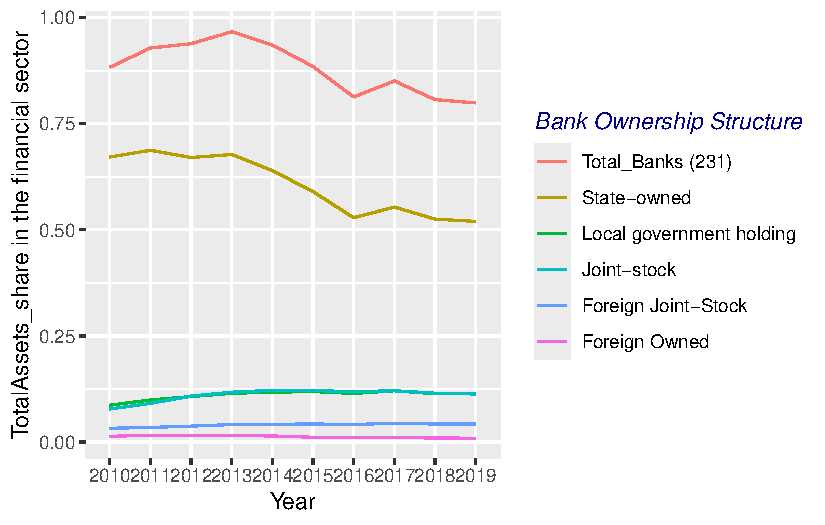
\includegraphics{chapter00-landscape_banking_files/figure-pdf/fig-AssetsOwnership-1.pdf}

}

\caption{\label{fig-AssetsOwnership}Banks' Total Assets - by Ownership
Structure (2010-2019)}

\end{figure}%

In the appendix (Table~\ref{tbl-appendixAssets}), the total assets of
the state-owned banks show the absolute decrease pattern (from 67.18\%
to 51.99\%); in other subsectors, due to their overall increase in the
total assets, the state-owned institutions in those subsectors exhibit a
relative decrease. The same descending tendency can be found in Hsiao et
al. (2015) where the share of total assets of the biggest five banks
(the state-owned banks) decreased from 61.83\% to 52.76\% during
2007-2012; and the joint-stock banks increased gradually. Other
ownership structures, especially local-government holding, joint-stock
and foreign joint-stock, all reveal an obvious increase trend. For
example, the total assets of the joint-stock insurance companies have
leaped from 0.45\% in 2010 to 1.7\% in 2019.

Figure~\ref{fig-AssetsOwnership} demonstrates the change of the banks'
total assets by different ownership structures. Apart from the clear
decrease of the portion of the state-owned, the total assets of the
joint-stock and the local-government holding banks gradually increased.
Another type of ownership structure -- foreign joint-stock banks show
similar tendency to the local-government holding banks, with the share
going up from 3.26\%\% in 2010 to 4.27\% in 2015 and remaining steady
since then. However, the foreign-owned banks' share has slightly dropped
from 1.38\% in 2010 to 0.92\%\% in 2019. The reasons behind the patterns
exhibited in Figure~\ref{fig-AssetsOwnership} might be closely related
to a series of strategies of Chinese government and the regulatory
authorities after China's accession to the WTO in 2001 such as
regulations concerning the diversifying the shareholders of commercial
banks.

\subsection{Financial Ratios of CAMELS rating
system}\label{financial-ratios-of-camels-rating-system}

Following the ratio classification used by the CAMELS rating system, we
analyze the financial ratios of 233 sample banks, in terms of their
ownership structures and the bank types. CAMELS rating system is the
common name for the Uniform Financial Institutions Rating System (UFIRS)
which was first adopted by the Federal Reserve U.S. in 1979 as a
methodology to evaluate the soundness and safety of depository
institutions. The `CAMELS' is an acronym of the six assessment
components: Capital adequacy, Asset quality, Management, Earnings,
Liquidity and Sensitivity to Market Risk. The Sensitivity to Market Risk
was added into the UFIRS in 1996 as an evaluation component.\footnote{The
  CAMELS rating system evaluates a bank's strength across six key
  categories: capital adequacy, assets, management capability, earnings,
  liquidity, and sensitivity. For more detailed information, see Federal
  Reserve website and the Commercial Bank Examination Manual
  \url{https://www.federalreserve.gov/publications/files/cbem.pdf}.} In
this sector, we use the CAMEL ratios to assess the safety and soundness
of the sample banks on the ground that the Sensitivity component
requires market data which are not available for those non-listed banks.
Due to the fact that the CAMELS rating system guidance only gives the
principle guidelines of the above assessment factors instead of the
exact financial ratios, we take the following financial ratios as the
factors for evaluating the safety and soundness of the sample banks, by
reference to the relevant literature such as Gunther and Moore (2003),
Arena (2008), and Bitar et al. (2018). Variable definitions and the
definition source are listed in appendix Table~\ref{tbl-CAMELvariables}.

\subsubsection{\texorpdfstring{\emph{CAMEL Ratios of Commercial banks --
Capital
Adequacy}}{CAMEL Ratios of Commercial banks -- Capital Adequacy}}\label{camel-ratios-of-commercial-banks-capital-adequacy}

\begin{figure}

\centering{

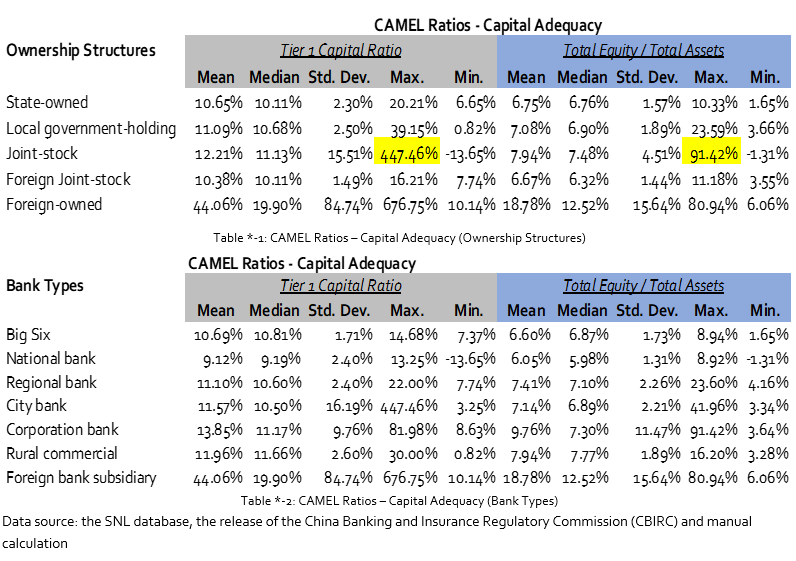
\includegraphics[width=0.7\textwidth,height=\textheight]{chapter00-landscape-capital_statistics.png}

}

\caption{\label{fig-CAMELcapital}CAMEL Ratios-Capital Adequacy}

\end{figure}%

\begin{figure}

\centering{

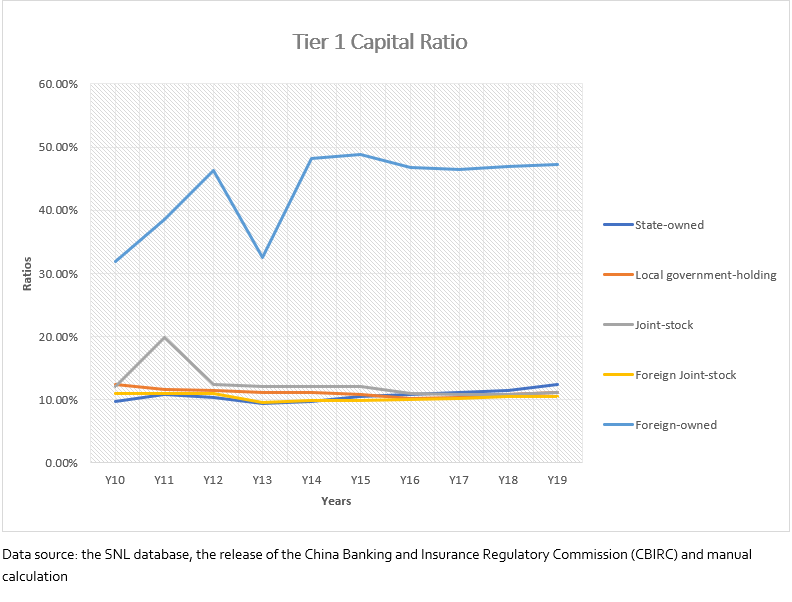
\includegraphics[width=0.7\textwidth,height=\textheight]{chapter00-landscape-Tier1.png}

}

\caption{\label{fig-CAMELTier1}The Yearly Mean of Tier1 Capital Ratios
(Ownership Structure)}

\end{figure}%

We examine two capital adequacy ratios: Tier 1 capital ratio and Total
equity to total assets ratio. Except for the foreign banks, the means of
Tier 1 capital ratio of other different types of banks are quite close,
from 10.64\% to 12.21\%. The state-owned banks have the mean of 10.65\%.
The joint-stock banks have the highest mean of Tier 1 capital ratio
which is 12.21\% and have the highest standard deviation of 15.51\%.
This might be due to that joint-stock banks are quite different from
each other in sizes, performance, and risk management competence, as
well as the abnormal maximum value of 447.46\%. These results are
corroborated by the Table 3-2 categorized by bank types. Apart from the
state-owned Big Six being consistent with the mean of the state-owned
banks, national banks show a mean of the state-owned banks, the local
government holding banks, and the joint-stock banks, since there are 12
national banks and comprised with the abovementioned ownership
structure. Most regional banks are involved with local government
shareholders, city banks and rural commercial banks are mostly
joint-stock banks, therefore their means are close to the means of those
ownership structures. Corporation banks \footnote{Regional banks and
  Corporation banks will be combined with the category of ``City bank''
  in the following capters because of their similar sizes, business
  lines, and the places where the banks operate.} are the banks which
were funded initially by some corporations or companies in order to
provide financial services for the specific industries, and emerged
after 2015. Therefore, these banks are similar to the joint-stock banks
in terms of sizes and geographic areas. There are 13 corporation banks
by the end of 2019, including those founded by the private companies.
The China Banking Regulatory Commission (CBRC) issued `Commercial Bank
Capital Management Measures (Trial)' in 2012, which is the sign of the
adoption of Basel III, demanding that all commercial banks in China
would have to apply the new capital adequacy requirements under Basel
III since 2013. As a result, the value of Tier 1 ratio of all ownership
structure decreased compared to the previous year. As shown in
Figure~\ref{fig-CAMELTier1}, since 2013, the Tier 1 capital ratio of all
types of banks have been increasing gradually.

The ratio of total equity/total assets represents the book value
leverage of a bank. The majority of means of total equity/total assets
of banks with different ownership are below 8\% yet over 6.50\%, such as
local government holding banks at 7.08\%, slightly higher than the
state-owned banks (6.76\%). However, the mean of the ratio of
joint-stock banks are almost 13\% higher than other types of banks. A
higher of standard deviation of the ratio (4.51\%) might reveal the
cause of a higher mean of the joint-stock banks. The peer group of Bank
Types provides the corresponding results. As presented in
Figure~\ref{fig-CAMELTE}, The yearly mean of the ratio of total
equity/total assets have shown different trends between different types
of ownership. Except that the state-owned banks have been following
gradual growth year by year, other bank types have exhibited the
tendency of increase-decrease-increase again. The yearly mean of the
ratio of all banks are over 7\% in 2019.

The foreign-owned banks have displayed abnormally high capital adequacy
ratios. We cannot trace the values back to its sources due to the data
availability. Speculatively, this might be caused by a relatively small
size of the assets of the foreign-owned banks in China.

\begin{figure}

\centering{

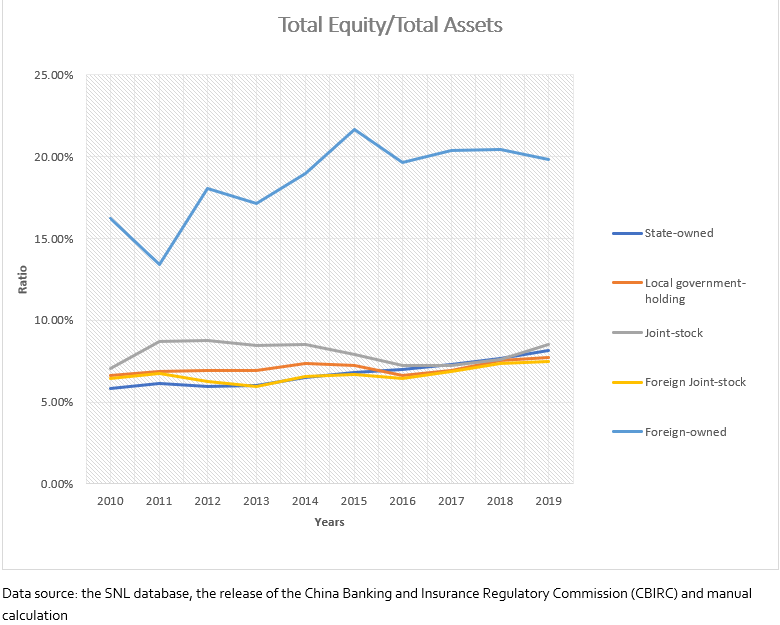
\includegraphics[width=0.7\textwidth,height=\textheight]{chapter00-landscape-TEtoTA.png}

}

\caption{\label{fig-CAMELTE}The Yearly Mean of Total Equity/Total Assets
(Ownership Structure)}

\end{figure}%

\begin{figure}

\centering{

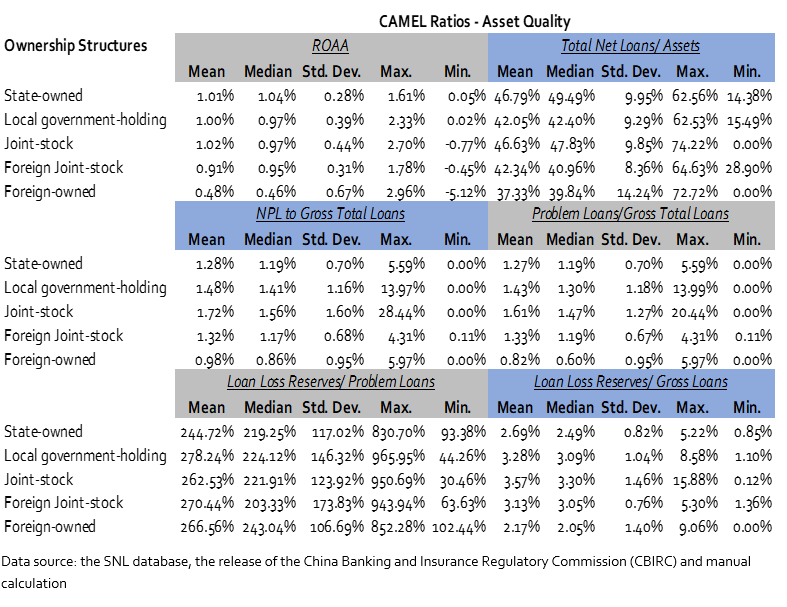
\includegraphics[width=0.7\textwidth,height=\textheight]{chapter00-landscape-asset_quality.png}

}

\caption{\label{fig-CAMELAQ}CAMEL Ratios-Asset Quality (Ownership
Structure)}

\end{figure}%

\begin{figure}

\centering{

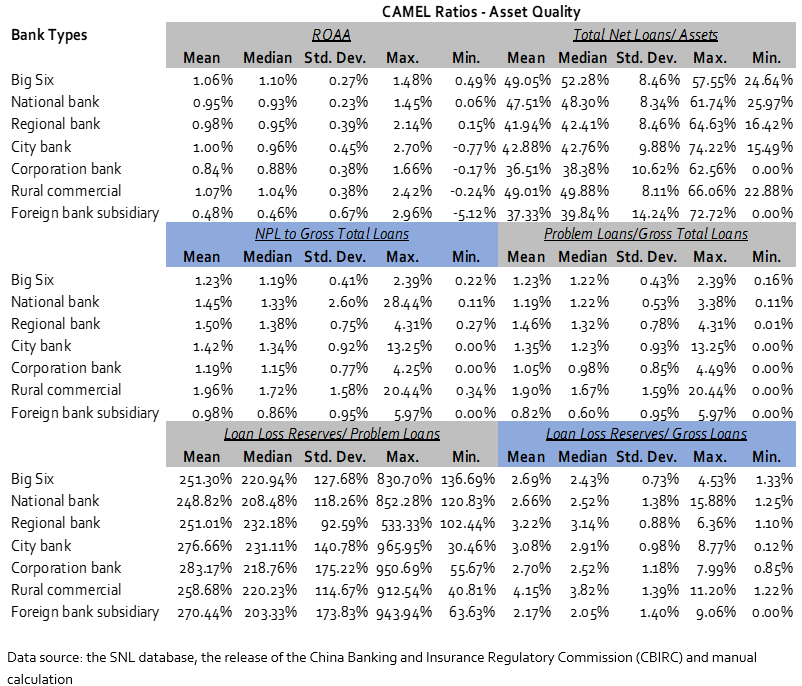
\includegraphics[width=0.7\textwidth,height=\textheight]{chapter00-landscape-asset_quality_1.png}

}

\caption{\label{fig-CAMELAQ1}CAMEL Ratios-Asset Quality (Bank Type)}

\end{figure}%

\begin{figure}

\centering{

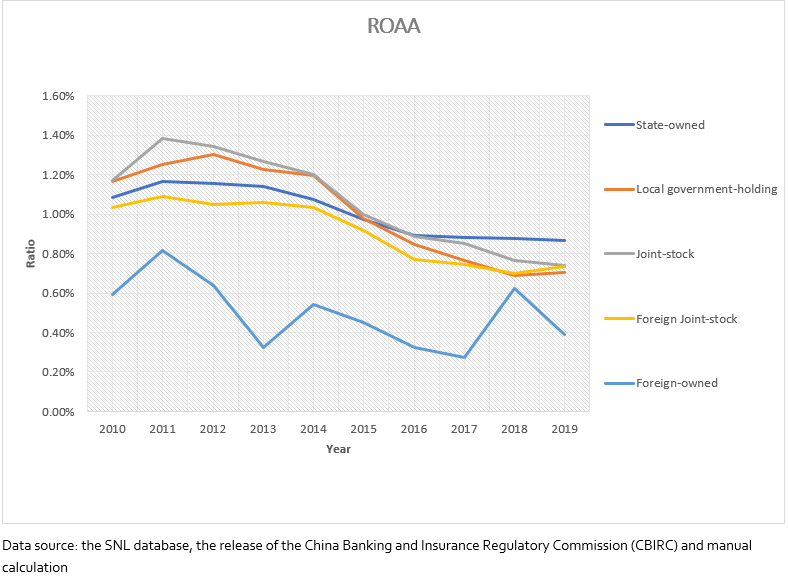
\includegraphics[width=0.7\textwidth,height=\textheight]{chapter00-landscape-ROAA.png}

}

\caption{\label{fig-ROAA}The Yearly Means of ROAA (Ownership Structure)}

\end{figure}%

The ratio of return on average assets (ROAA), the ratios associated with
Non-performing Loans (NPLs to total loans, problem loans/total loans,
loan loss reserves/problem loans and loan loss reserves/gross loans) and
the ratio of net loans/total assets constitute the assessment of asset
quality of banks.

The means and medians of ROAA of different ownership structure are
centered around 1\%, with the exception of the foreign owned banks at
0.48\%, almost only as half of the other types of banks. This might be
due to the high costs of the foreign-owned banks' operation in China's
financial markets and could also collaborate with the ratio of Cost to
Income in the later part of analysis. In the peer group of Bank Types,
the Big Six has the highest ROAA ratio, which might reveal the economies
of scale. Figure~\ref{fig-ROAA} displays that the yearly means have a
trend of decline since 2012/2013, which could reveal the
disproportionate growth of return and the total assets of banks in
recent years and could also reveal the competition rising in the banking
industry.

The ratios associated with Non-Performing Loans (NPLs) can be divided
into two groups with regards to their indications, like two sides of a
coin. The group of the ratio of NPLs to total loans and the ratio of
problem loans/total loans indicates the issue of problematic loans.
Intuitively the lower the ratios are, the better the asset quality is.
The group of the ratios of loan loss reserves/problem loans and loan
loss reserves/gross loans means the safeguards a bank puts into its
dubious loans, the higher the better. The results are consistent with
the country NPL results from the IMF Financial Soundness Indicators for
Global Financial Stability Report (2019) that China's commercial banks
have a relatively low rate of NPL. The reason attributed will be
explained later. In the above table, the state-owned banks exhibit the
lowest means of NPLs to total loans and problem loans/total loans
(1.28\% and 1.27\%, respectively) amongst all ownership structures. In
terms of bank types, the rural commercial banks have the highest NPL to
Gross Loan rate and the ratio of Problem Loans/Gross Total Loans, being
1.96\% and 1.9\% respectively, which is consistent with the higher
credit risk that small and medium banks are facing. Although rural
commercial banks also have the highest Loan Loss Reserves/Gross Loans
rate as 4.51\%, the relatively low ratio of Loan Loss Reserves/Problem
Loans, being 258.65\%, potentially means that rural commercial banks
might not have enough safeguards against the default risk. The yearly
mean of NPLs to total loans (Figure~\ref{fig-NPL}) exhibit total
increase during 2010-2018 in all ownership structures except for
foreign-owned banks, revealing the highest mean of NPLs to total loans
by 2.44\% of the joint-stock banks. The foreign owned banks demonstrate
the descending trend since 2013, the reason possibly relates to their
business focus differing from other domestic banks.

\begin{figure}

\centering{

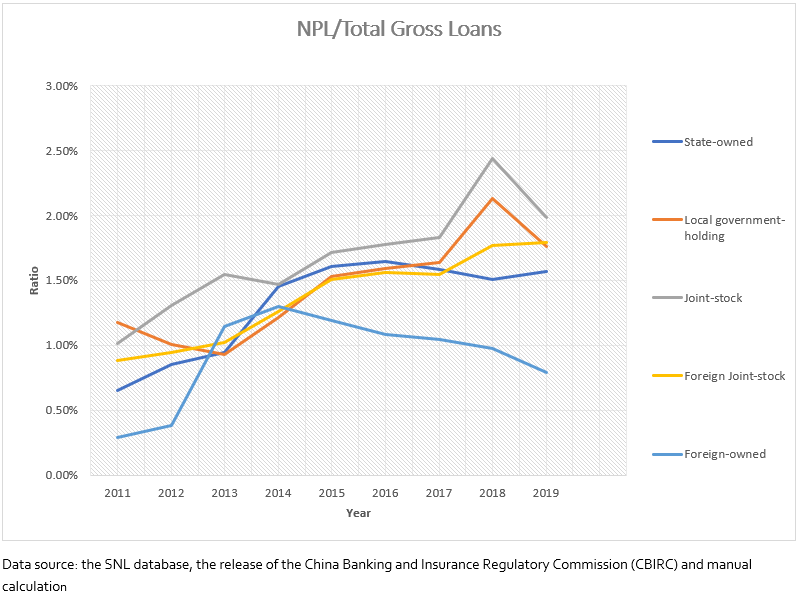
\includegraphics[width=0.7\textwidth,height=\textheight]{chapter00-landscape-NPL.png}

}

\caption{\label{fig-NPL}The Yearly Means of NPL/Total Gross Loans
(Ownership Structure)}

\end{figure}%

The IMF Financial Soundness Indicators for Global Financial Stability
Report (2019) reveals that China has a relatively lower NPL ratio (NPLs
to total loans) than most members of G20 countries, especially lower
than those developing countries, despite increasing overall since 2010
(See Part II, Figure~\ref{fig-shadowbanking}). One reason could be
attributed to China's financial reform. During the transformations of
the Big Six and the city banks, the asset management companies,
including the four national ones and those local asset management
institutions bought a great amount of NPLs of banks and move them off
the banks' balance sheets. Another effective solution is that the
mergers and consolidations of formal city cooperatives after China's
accession to the WTO in 2001. The NPLs which might have been held by
city cooperative reciprocally could been restructured and deducted from
the consolidated balance sheets when the new city banks were
established. Besides, the NPLs might have been reduced or restructured
in the process of introducing new non-financial institutional
shareholders such as private companies. Along with the business
solutions for NPLs, the stringent regulation and supervision upon the
NPLs quotas by the CBIRC also help restraining the ratio under limits.
The Law of the People's Republic of China on Banking Supervision and
Administration stipulates that banks' violation by covering up NPLs or
inaccurate classification of NPLs would face official censure. Zhang et
al. (2016) provides evidence that the restrictions on NPLs by the CBIRC
and the capital injection by the government in order to control the NPL
level.

\begin{figure}

\centering{

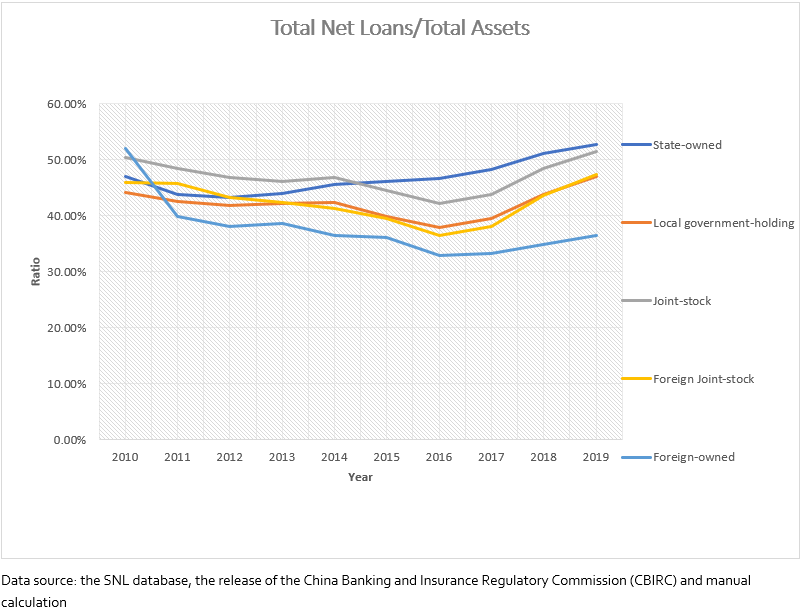
\includegraphics[width=0.7\textwidth,height=\textheight]{chapter00-landscape-NLtoTA.png}

}

\caption{\label{fig-NLtoTA}The Yearly Means of Total Net Loans/Total
Assets (Ownership Structure)}

\end{figure}%

The last ratio in assessing asset quality is net loans/total assets. The
state-owned banks and the joint-stock banks have the close means of this
ratio at 46.79\% and 46.63\% respectively; while the similar means are
held by the local government holding banks and the foreign joint-stock
banks around 42\%. The foreign owned banks, however, have a lower mean
of net loans/total assets by 37.33\%, which is probably due to the
smaller size of loans of the foreign owned banks compared to domestic
banks, although the restriction upon local currency banking business had
been lifted entirely since 2006. Figure~\ref{fig-NLtoTA} discloses that
the yearly variance of net loans/total assets of all ownership
structures are not significant from a long-term perspective, which might
indicate that the relatively proportional changes between net loans and
the total assets of banks.

\subsubsection{\texorpdfstring{\emph{CAMEL Ratios of commercial banks --
Management
Quality}}{CAMEL Ratios of commercial banks -- Management Quality}}\label{camel-ratios-of-commercial-banks-management-quality}

\begin{figure}

\centering{

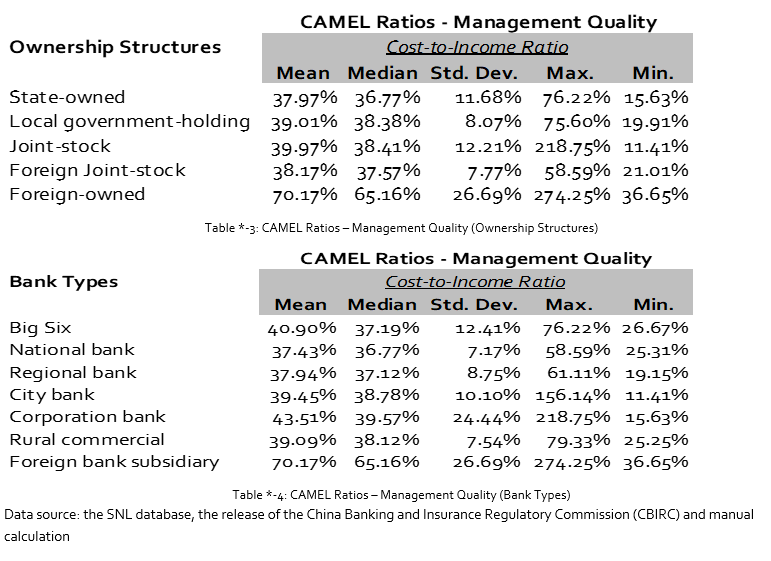
\includegraphics[width=0.7\textwidth,height=\textheight]{chapter00-landscape-management_quality.png}

}

\caption{\label{fig-CAMELMQ}CAMEL Ratios -- Management Quality}

\end{figure}%

\begin{figure}

\centering{

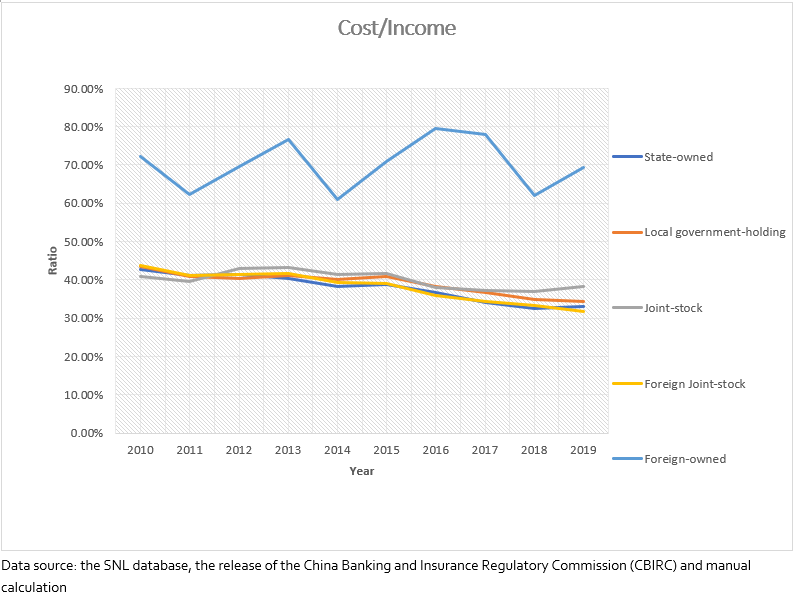
\includegraphics[width=0.7\textwidth,height=\textheight]{chapter00-landscape-Cost.png}

}

\caption{\label{fig-Cost}The Yearly Means of Cost/Income (Ownership
Structure)}

\end{figure}%

In the CAMEL rating system, management quality is evaluated by the ratio
of cost-to-income. Domestic banks have the similar cost-to-income ratios
in the range of over 37.9\% to nearly 40\%, with the state-owned banks
having the lowest at 37.97\% and the joint-stock banks having the
highest at 39.97\%. However, the foreign owned banks have almost twice
cost-to-income ratio as the domestic banks, presenting the number as
70.17\%. Bitar et al. (2018) examine 1992 banks in 39 OECD countries and
found the mean of cost-to-income ratio as 70.8\%. Comparing the value of
the cost-to-income ratio with the existing literature, it may imply that
the Chinese banks have a lower cost while the foreign owned banks have
the normal cost in their business. The results of the peer group of Bank
Types are consistent with that of Ownership Structures. The corporation
banks have the highest mean of this ratio as 43.51\%, which might due to
the facts that most of these banks are relatively new banks and have
specific geographic and/or industrial focuses. Apart from the
foreign-owned banks, the overall decreasing tendency of the movement of
the ratio has been displayed for all ownership structures through the
past 10 years (Figure~\ref{fig-Cost}). The fact that Chinese banks have
a lower cost might due to two main reasons. First, interest rates
including deposit and loan interest rates have been under the stringent
guidance, to a great extent, by the regulatory authorities (mainly the
central bank) for many years. This almost secures a certain amount of
cost and income of banks. Only by the recent years, the financial reform
initiatives concerning interest rates have been taking steps. It was
only since 2013 that the Loan Prime Rate (LPR)\footnote{Loan Prime Rate
  (LPR) is one of the essential initiatives of interest rate reform in
  China's financial markets. It resembles the Libor, as a basic interest
  rate in loan markets, quoted by 18 major commercial banks on monthly
  basis.} has been set up and since 2019 put into effect. Second, the
increase of income, including interest income and non-interest income,
is faster than the increase of costs of banks through the past 10 years,
which matches the fast pace of China's economic development.

\subsubsection{\texorpdfstring{\emph{CAMEL Ratios of commercial banks --
Earnings}}{CAMEL Ratios of commercial banks -- Earnings}}\label{camel-ratios-of-commercial-banks-earnings}

\begin{figure}

\centering{

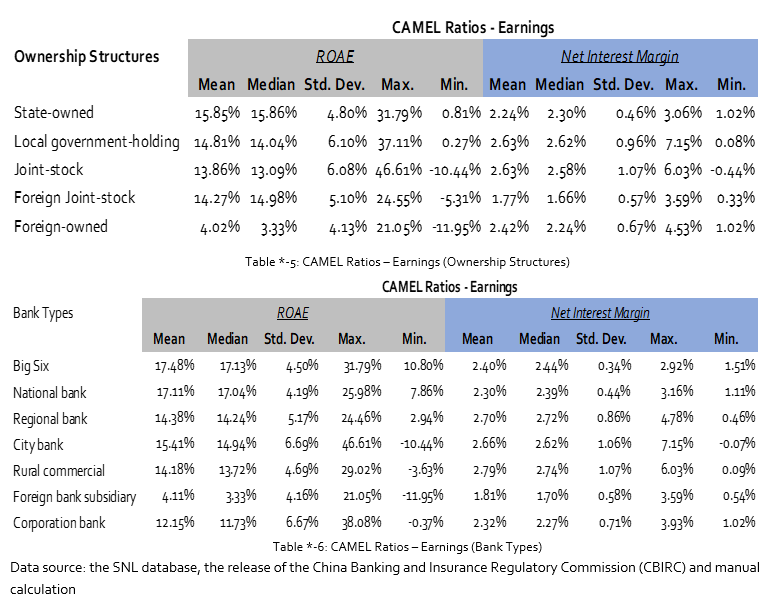
\includegraphics[width=0.7\textwidth,height=\textheight]{chapter00-landscape-earnings.png}

}

\caption{\label{fig-CAMELearnings}CAMEL Ratios -- Earnings}

\end{figure}%

Usually Return on Average Equity (ROAE) and net interest margin are used
to measure the quality of banks' earnings. The ratios are expected to be
positively associated with banks' profitability, as the higher the
better, intuitively.

The means of ROAE of the state-owned banks and the local-government
holding banks are higher, being 15.85\% and 14.81\% respectively; while
the joint-stock banks are 2\% lower than their aforementioned
counterparties. The foreign owned banks have a mean of 4.02\% of ROAE.
Although the state-owned banks have the highest ROAE, their net interest
margin is not the highest. The local government holding and the
joint-stock banks have the highest means of net interest margin at
2.63\%. As for the bank types, the Big Six definitely have the highest
ROAE rate as 16.9\%, while a relatively lower net interest margin ratio
as 2.36\% than regional banks, city banks, and rural commercial banks.
Considering these two ratios together, the reason that the foreign owned
banks are lagged by the domestic banks could be due to the small size of
their interest-bearing business in China's financial markets. The fact
that the state-owned banks have a higher ROAE and a lower net interest
margin could be attributed to their clientele and business
diversification. Most state-owned banks are national banks which target
national state-owned and private corporations and conglomerates as their
clientele. However, local government holding banks, joint-stock banks
and foreign joint-stock banks are mostly regional banks, city banks or
rural commercial banks which act as the major finance provider for the
regional, small and medium sized business and individuals within their
local communities. It is a consensus opinion that big companies usually
have more power in negotiation with banks than those small and medium
sized companies and individuals. Therefore, the (loan) interest income
of the state-owned banks probably could be lower than those local
community banks. Business diversification of Chinese banks emerged
around the end of the last century when China was making progress on the
commitment to the WTO agreement. The People's Bank of China (PBOC)
issued regulatory documents lifting the restrictions on market entry for
domestic banks in 2002. Berger et al. (2010) illustrate Big Six
established their branches across all the regions in China during this
period. Alongside with the regional expansion, non-interest-bearing
business started to be prospective during this period in China's
financial reform. The PBOC also released regulatory documents about
easing the restriction on fee-based banking business and allowed banks
to cooperate with insurance companies and other banking institutions
such as trust companies. Yuan (2006) and Berger et al. (2010) both
mentioned national banks embarked on non-interest bearing business
including cash management, wealth management, trading services etc.
Business diversification of those state-owned, national banks caused the
proportion of interest-bearing business to assets relatively to
decrease, which can explain why the state-owned banks have a lower net
interest margin compared to their peers. As for local banks including
local government holding, joint-stock and foreign joint-stock banks,
their business diversification started later than the national banks.
Taking account of their clientele and their service region, it might be
reasonable to assume that their business still relies more on
interest-bearing assets than the state-owned banks.

\subsubsection{\texorpdfstring{\emph{CAMEL Ratios of commercial banks --
Liquidity}}{CAMEL Ratios of commercial banks -- Liquidity}}\label{camel-ratios-of-commercial-banks-liquidity}

\begin{figure}

\centering{

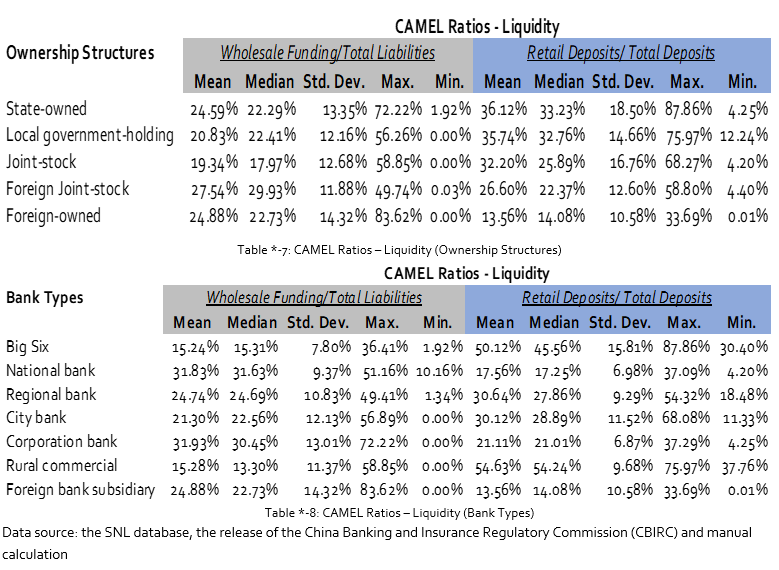
\includegraphics[width=0.7\textwidth,height=\textheight]{chapter00-landscape-liquidity.png}

}

\caption{\label{fig-CAMELliquidity}CAMEL Ratios -- Liquidity}

\end{figure}%

The CAMELS rating system concerning liquidity evaluates the competence
of banks in asset and liability management (ALM) which encompasses
interest rate risk and liquidity risk. Here we choose to focus on
liquidity risk since interest rate risk of China's banks might be
relatively under control guided by the regulatory authorities. The
ratios of wholesale funding/total liabilities and retail deposits/total
deposits can represent the current level of liquidity and the volatility
of the funding sources. Demirgüç-Kunt and Huizinga (2010) present
evidence that wholesale funding may increase banks' risk, such as stock
volatility, although it supports large banks' fast expansion. As to
retail deposits, Hirtle and Stiroh (2007) state that retail deposits may
provide a more stale business line for banks, although they may have
lower returns.

The state-owned banks, foreign joint-stock banks and foreign owned banks
have higher means of the ratio of wholesale funding/total liabilities,
with 24.59\%, 27.54\% and 24.88\% respectively. While the means of the
local government holding banks and the joint-stock banks are almost
3-4\% lower than the state-owned banks, with 20.83\% and 19.34\%
respectively. The lower means mostly belong to those city banks and
rural commercial banks whose ownership structure are local government
holding and joint-stock. These small and medium sized banks, consistent
with the statement of the existing literature, focus on serving their
local communities and might have more conservative strategy of business
expansion. The results presented in Table 7-2 confirmed this assumption.
The city banks and the rural commercial banks have the means of the
ratio of wholesale funding/total liabilities of 15.28\% and 21.31\%
respectively, the lowest value in the peers. On the other hand, the
national banks and regional banks have the highest values of 31.83\% and
24.74\% respectively, which means that these banks might face more
liquidity risk than the rest of their peers.

The ratio of retail deposits/total deposits might be less indicative of
banks' funding source reliance due to the fact that there are less
observations available on this variable. However, the results may still
corroborate the means of wholesale funding/total liabilities to the
great extent. The local government holding banks and the joint-stock
banks have a relatively high ratio of retail deposit/total deposit at
35.74\% and 32.20\%; while foreign joint-stock and foreign owned banks
have a ratio of 5-10\% lower. Foreign owned banks have the lowest ratio
of 13.56\%, which could imply that foreign owned banks might not take
retail deposit strategy in China's financial markets. The state-owned
banks, however, have the highest ratio of 36.12\%; and the Big Six have
the consistent value of 50.12\%. The reasons could be traced to
historical and diversification rationales. First, the state-owned banks,
especially the Big Four, were the earliest commercial banks in China and
entirely owned and controlled by the state government. Before
legislation of deposit insurance was implemented in 2015, the state
government in fact took the role of the implicit deposit insurer. As a
long-term habit and due to trust, Chinese individuals, especially
residents in cities, still consider these state-owned, large banks as
their first choice for deposits and wealth management, even though there
are numerous commercial banks. Second, the state-owned banks achieved
more in geographical expansion and business diversification than city
banks, in relation to time, scope and depth. Combined with the first
reason, it is understandable that the state-owned banks have a higher
ratio. The rural commercial banks have a rather higher ratio of 54.63\%
than the Big Six, which is in accordance with their lower reliability to
the wholesale funding.

\subsubsection{\texorpdfstring{\emph{Conclusion}}{Conclusion}}\label{conclusion}

The CAMELS rating system is a popular methodology to assess the safety
and soundness of individual banks in the banking industry. Guided by the
CAMELS framework, this section presents an overview of China's banking
industry a quantitative perspective. Commercial banks have a capital
adequacy ratio over 10\% which is higher than the standard of Basel III
framework. The state-owned banks do not display the highest ratios.
China's banking industry has a lower average NPL ratio than other
members of G20 and has its own reasons. However, our analysis shows that
those small and medium banks might not have enough safeguards against
the relatively higher credit risk they are facing. China's commercial
banks have a lower cost to income ratio than foreign banks and the
average value in literature, mainly because of the stringent guidance on
interest rates in China's financial markets. The slow progress of the
reforms on market rates also have ensured, to a large degree of extent,
commercial banks have the ratio of return on equity over 14\% on
average. As for liquidity risk, the biggest and the smaller commercial
banks averagely do not highly rely on wholesale funding. Nevertheless,
the medium banks, especially those involved with local government
shareholders in history, might have higher liquidity risk because they
rely on wholesale funding channels more heavily.

\newpage

\section{Appendices}\label{appendices}

\subsection{Key regulation and regulatory documents in the adoption of
Basel III
framework}\label{key-regulation-and-regulatory-documents-in-the-adoption-of-basel-iii-framework}

\begingroup\fontsize{8}{10}\selectfont

\begin{longtable}[t]{l>{\raggedright\arraybackslash}p{6.5cm}>{\raggedright\arraybackslash}p{6.5cm}}

\caption{\label{tbl-regulatorydocs}Key regulation and regulatory
documents in the adoption of Basel III framework}

\tabularnewline

\toprule
\textbf{Date} & \textbf{Regulation Documents} & \textbf{Regulatory Objectives}\\
\midrule
\endfirsthead
\multicolumn{3}{@{}l}{\textit{(continued)}}\\
\toprule
\textbf{Date} & \textbf{Regulation Documents} & \textbf{Regulatory Objectives}\\
\midrule
\endhead

\endfoot
\bottomrule
\endlastfoot
\cellcolor{gray!10}{June 2012} & \cellcolor{gray!10}{Commercial Bank Capital Management Measure (Trial)} & \cellcolor{gray!10}{Fully adoption of the core elements of the Basel III framework}\\
January 2014 & Notice on Issuing the Guidelines for Disclosure of Global System Importance Assessment Indicators of Commercial Banks & Participation of the assessing process of the Globally Systemically Important Banks\\
\cellcolor{gray!10}{January 2015} & \cellcolor{gray!10}{Commercial Banks' Leverage Management Measure (Revised)} & \cellcolor{gray!10}{Being consistent with the requirements on leverage ratios in the Basel III framework}\\
December 2015 & Commercial Bank's Liquidity Coverage Information Disclosure Measures & Adoption of the Pillar III - Market Dicipline\\
\cellcolor{gray!10}{April 2017} & \cellcolor{gray!10}{Commercial Bank Collateral Management Guidelines} & \cellcolor{gray!10}{Elaborating the detailed requirements on credit risk}\\
\addlinespace
January 2018 & Derivative Counterparty Default Risk Exposure Measurement Rules & Focusing on Counterparty Risk\\
\cellcolor{gray!10}{April 2018} & \cellcolor{gray!10}{Measurement of Large Exposure of Commercial Banks} & \cellcolor{gray!10}{Implementation of the large exposure framework}\\
May 2018 & Commercial Bank Liquidity Risk Management Measurement (Revised) & Updating the regulation on liquidty risk\\
\cellcolor{gray!10}{March 2019} & \cellcolor{gray!10}{Commercial Banks' Net Stable Funding Ratio Information Disclosure Rules} & \cellcolor{gray!10}{Updating the regulation on liquidty risk}\\*

\end{longtable}

\endgroup{}

\subsection{CAMEL variable definition and data
source}\label{camel-variable-definition-and-data-source}

\begingroup\fontsize{8}{10}\selectfont

\begin{longtable}[t]{>{\raggedright\arraybackslash}p{5cm}>{\raggedright\arraybackslash}p{8cm}l}

\caption{\label{tbl-CAMELvariables}Summary of CAMEL Variable Definitions
and Source}

\tabularnewline

\toprule
\textbf{Variable} & \textbf{Definition} & \textbf{Definition  Source}\\
\midrule
\endfirsthead
\multicolumn{3}{@{}l}{\textit{(continued)}}\\
\toprule
\textbf{Variable} & \textbf{Definition} & \textbf{Definition  Source}\\
\midrule
\endhead

\endfoot
\bottomrule
\endlastfoot
\addlinespace[0.3em]
\multicolumn{3}{l}{\textbf{Capital Adequacy}}\\
\hspace{1em}\cellcolor{gray!10}{Tier 1 Ratio} & \cellcolor{gray!10}{Tier 1 capital as a percent of risk-weighted assets as defined by the latest regulatory guidelines} & \cellcolor{gray!10}{SNL database}\\
\hspace{1em}Total Equity/Total Assets & Equity as a percent of assets & SNL database\\
\addlinespace[0.3em]
\multicolumn{3}{l}{\textbf{Asset Quality}}\\
\hspace{1em}\cellcolor{gray!10}{ROAA} & \cellcolor{gray!10}{Return on average assets; net income as a percent of average assets} & \cellcolor{gray!10}{SNL database}\\
\hspace{1em}NPL /Gross Total Loans & Nonperforming loans, net of guaranteed loans, as a percent of loans before reserves & SNL database\\
\hspace{1em}\cellcolor{gray!10}{Problem Loans / Gross Total Loans} & \cellcolor{gray!10}{Problem loans as a percent of gross total loans} & \cellcolor{gray!10}{SNL database}\\
\hspace{1em}Loan Loss Reserves / Problem Loans & Loan loss reserves as a percent of problem loans & SNL database\\
\hspace{1em}\cellcolor{gray!10}{Loan Loss Reserves /Gross Loans} & \cellcolor{gray!10}{Loan loss reserves as a percent of gross loans. Gross loans are as reported on the balance sheet and may be derived from total gross loans or amortized gross customer loans} & \cellcolor{gray!10}{SNL database}\\
\hspace{1em}Total Net Loans / Total Assets & Loans and finance leases, net of loan-loss reserves, as a percent of assets & SNL database\\
\addlinespace[0.3em]
\multicolumn{3}{l}{\textbf{Management Quality}}\\
\hspace{1em}\cellcolor{gray!10}{Cost/Income} & \cellcolor{gray!10}{Expense as a percent of revenue; i.e. efficiency ratio - Noninterest expense before foreclosed property expense, amortization of intangibles, and goodwill impairments as a percent of net interest income (fully taxable equivalent, if available) and noninterest revenues, excluding only gains from securities transactions and nonrecurring items.} & \cellcolor{gray!10}{SNL database}\\
\addlinespace[0.3em]
\multicolumn{3}{l}{\textbf{Earnings}}\\
\hspace{1em}ROAE & Return on average equity; net income as a percent of average equity & SNL database\\
\hspace{1em}\cellcolor{gray!10}{Net Interest Margin} & \cellcolor{gray!10}{Net interest income, on a fully taxable-equivalent basis if available, as a percent of average earning assets. If average earning assets is not available, average financial assets may be used.} & \cellcolor{gray!10}{SNL database}\\
\addlinespace[0.3em]
\multicolumn{3}{l}{\textbf{Liquidity}}\\
\hspace{1em}Wholesale Funding / Liabilities (WF to Liabilities) & Wholesale funding including financial liabilities and repurchase agreements, excluding derivatives and customer deposits, as percentage of liabilities & SNL database\\
\hspace{1em}\cellcolor{gray!10}{Retail Deposits / Deposits} & \cellcolor{gray!10}{Retail deposits as a percent of retail and corporate deposits} & \cellcolor{gray!10}{SNL database}\\*

\end{longtable}

\endgroup{}

\subsection{Total Assets of the Banking
Sector}\label{total-assets-of-the-banking-sector}

\begingroup\fontsize{8}{10}\selectfont

\begin{longtable}[t]{lrrrrrrrrrr}

\caption{\label{tbl-appendixAssets}Total Assets Shares in the Financial
Sector - detailed by Ownership Structure (2010-2019)}

\tabularnewline

\toprule
Ownership & 2019 & 2018 & 2017 & 2016 & 2015 & 2014 & 2013 & 2012 & 2011 & 2010\\
\midrule
\endfirsthead
\multicolumn{11}{@{}l}{\textit{(continued)}}\\
\toprule
Ownership & 2019 & 2018 & 2017 & 2016 & 2015 & 2014 & 2013 & 2012 & 2011 & 2010\\
\midrule
\endhead

\endfoot
\bottomrule
\multicolumn{11}{l}{\rule{0pt}{1em}\textit{Data source: }}\\
\multicolumn{11}{l}{\rule{0pt}{1em}the SNL database, the release of the China Banking and Insurance Regulatory Commission (CBIRC) and manual calculation}\\
\endlastfoot
\addlinespace[0.3em]
\multicolumn{11}{l}{\textbf{Banks}}\\
\hspace{1em}Total\_Banks (231) & 0.7990 & 0.8068 & 0.8509 & 0.8132 & 0.8849 & 0.9355 & 0.9668 & 0.9386 & 0.9285 & 0.8830\\
\hspace{1em}State-owned & 0.5199 & 0.5253 & 0.5537 & 0.5286 & 0.5901 & 0.6395 & 0.6776 & 0.6704 & 0.6874 & 0.6717\\
\hspace{1em}Local government holding & 0.1139 & 0.1140 & 0.1209 & 0.1145 & 0.1192 & 0.1175 & 0.1150 & 0.1072 & 0.0994 & 0.0869\\
\hspace{1em}Joint-stock & 0.1133 & 0.1152 & 0.1210 & 0.1187 & 0.1215 & 0.1219 & 0.1176 & 0.1084 & 0.0912 & 0.0780\\
\hspace{1em}Foreign Joint-Stock & 0.0427 & 0.0426 & 0.0445 & 0.0414 & 0.0427 & 0.0420 & 0.0413 & 0.0376 & 0.0346 & 0.0326\\
\hspace{1em}Foreign Owned & 0.0092 & 0.0097 & 0.0107 & 0.0100 & 0.0114 & 0.0145 & 0.0154 & 0.0149 & 0.0159 & 0.0137\\
\addlinespace[0.3em]
\multicolumn{11}{l}{\textbf{Insurance Companies}}\\
\hspace{1em}Total\_Insurance (37) & 0.0888 & 0.1008 & 0.1032 & 0.0957 & 0.1018 & 0.1017 & 0.1014 & 0.0911 & 0.0875 & 0.0698\\
\hspace{1em}State-owned & 0.0647 & 0.0772 & 0.0782 & 0.0668 & 0.0740 & 0.0784 & 0.0797 & 0.0795 & 0.0768 & 0.0602\\
\hspace{1em}Joint-stock & 0.0170 & 0.0167 & 0.0172 & 0.0152 & 0.0149 & 0.0146 & 0.0140 & 0.0049 & 0.0048 & 0.0044\\
\hspace{1em}Foreign Joint-Stock & 0.0023 & 0.0022 & 0.0021 & 0.0081 & 0.0069 & 0.0028 & 0.0018 & 0.0015 & 0.0014 & 0.0013\\
\hspace{1em}Private & 0.0048 & 0.0047 & 0.0057 & 0.0056 & 0.0059 & 0.0059 & 0.0059 & 0.0052 & 0.0045 & 0.0039\\
\addlinespace[0.3em]
\multicolumn{11}{l}{\textbf{Securities Companies}}\\
\hspace{1em}Total\_Securities (44) & 0.0252 & 0.0242 & 0.0270 & 0.0255 & 0.0304 & 0.0234 & 0.0134 & 0.0109 & 0.0117 & 0.0161\\
\hspace{1em}State-owned & 0.0062 & 0.0059 & 0.0063 & 0.0049 & 0.0049 & 0.0037 & 0.0020 & 0.0017 & 0.0018 & 0.0029\\
\hspace{1em}Local government holding & 0.0076 & 0.0074 & 0.0085 & 0.0086 & 0.0111 & 0.0087 & 0.0050 & 0.0039 & 0.0041 & 0.0057\\
\hspace{1em}Joint-stock & 0.0101 & 0.0098 & 0.0110 & 0.0116 & 0.0139 & 0.0106 & 0.0062 & 0.0050 & 0.0053 & 0.0071\\
\hspace{1em}Foreign Joint-Stock & 0.0012 & 0.0011 & 0.0011 & 0.0005 & 0.0005 & 0.0004 & 0.0003 & 0.0003 & 0.0004 & 0.0004\\
\hspace{1em}Private & 0.0000 & 0.0000 & 0.0000 & 0.0000 & 0.0000 & 0.0000 & 0.0000 & 0.0000 & 0.0000 & \vphantom{1} 0.0000\\
\addlinespace[0.3em]
\multicolumn{11}{l}{\textbf{Trust Companies}}\\
\hspace{1em}Total\_Trust (23) & 0.0016 & 0.0020 & 0.0022 & 0.0019 & 0.0021 & 0.0021 & 0.0019 & 0.0016 & 0.0014 & 0.0013\\
\hspace{1em}State-owned & 0.0003 & 0.0003 & 0.0004 & 0.0004 & 0.0004 & 0.0004 & 0.0004 & 0.0004 & 0.0003 & 0.0003\\
\hspace{1em}Local government holding & 0.0003 & 0.0003 & 0.0003 & 0.0003 & 0.0002 & 0.0002 & 0.0002 & 0.0002 & 0.0002 & 0.0002\\
\hspace{1em}Joint-stock & 0.0010 & 0.0010 & 0.0011 & 0.0009 & 0.0012 & 0.0011 & 0.0010 & 0.0008 & 0.0007 & 0.0007\\
\hspace{1em}Foreign Joint-Stock & 0.0001 & 0.0001 & 0.0001 & 0.0001 & 0.0001 & 0.0001 & 0.0001 & 0.0000 & 0.0000 & 0.0000\\
\hspace{1em}Foreign Owned & 0.0000 & 0.0003 & 0.0003 & 0.0002 & 0.0002 & 0.0002 & 0.0002 & 0.0002 & 0.0001 & 0.0001\\
\addlinespace[0.3em]
\multicolumn{11}{l}{\textbf{Specialty Lending Companies}}\\
\hspace{1em}Total\_Specialty\_Lending (6) & 0.0010 & 0.0011 & 0.0028 & 0.0015 & 0.0000 & 0.0012 & 0.0012 & 0.0010 & 0.0008 & 0.0006\\
\hspace{1em}State-Owned & 0.0010 & 0.0011 & 0.0019 & 0.0008 & 0.0000 & 0.0012 & 0.0012 & 0.0010 & 0.0008 & 0.0006\\
\hspace{1em}Joint-stock & 0.0000 & 0.0000 & 0.0008 & 0.0007 & 0.0000 & 0.0000 & 0.0000 & 0.0000 & 0.0000 & 0.0000\\
\hspace{1em}Private & 0.0000 & 0.0000 & 0.0000 & 0.0000 & 0.0000 & 0.0000 & 0.0000 & 0.0000 & 0.0000 & 0.0000\\*

\end{longtable}

\endgroup{}

\newpage

\subsection{Information of Basel
Accords}\label{information-of-basel-accords}

\textbf{\emph{Abstract and outlines}}:

This appendix is a description of relevant information about Basel
Accords (or Basel Framework). This appendix includes five sections.
Section I is the definition of Basel Accords and Basel Committee.
Section II briefly describes the development of Basel Framework
chronologically. Section III introduces the evolution of main parts of
Basel Framework from the perspective of risk-based categories. Section
IV describes the way of how Basel Framework functions. And section V is
to look ahead.

\subsubsection{What are Basel Accords?}\label{what-are-basel-accords}

Basel Accords are a series of financial regulations (including Basel I,
II and III) for the banking sector set by Basel Committee on Bank
Supervision (BCBS). Basel Accords, the prudential regulations reached by
the consensus of the worldwide central banks and bank supervisors, aim
to enhance the stability of the financial system as a whole. The risk
spectrum covered by Basel Accords concerns credit risk, market risk,
operational risk and other risks in banks and bank groups.

\begin{itemize}
\tightlist
\item
  Basel Committee on Bank Supervision (BCBS)
\end{itemize}

Basel Committee on Bank Supervision (thereafter BCBS, or Basel
Committee), founded in 1974, is one of the standard-setting committees
of the Bank for International Settlements (BIS). The BIS was established
in 1930 and owned by 60 central banks worldwide. The BIS has missions to
foster international cooperation in area of monetary and financial
stability and `act as a bank for central banks'({``About the BCBS,''}
2018).

Under this premise, the BCBS was established to act as an international
financial standard setter, as well as a provider of the forum for
communication and cooperation on banking supervision between its 45
member institutions from 28 jurisdictions ({``About the BCBS,''} 2018).

\subsubsection{The brief history of Basel
Accords}\label{the-brief-history-of-basel-accords}

Banks are highly leveraged institutions, which means that the banking
industry is borne to be highly profitable at the same time highly
fragile. The bank regulations have been existed since banks have been in
their current institutional forms (Barth et al., 2004). For example, in
the United States, the 1933 Banking Act not only imposed federal
oversight on commercial banks for the first time, but also established a
government corporation, the Federal Deposit Insurance Corporation (FDIC)
to protect the benefits of depositors in the U.S. commercial banks and
other saving institutions.

\begin{itemize}
\tightlist
\item
  Basel I
\end{itemize}

The highly unrestricted business expansion and the debacle of Latin
American debt crisis in the early 1980's highlighted the necessity of
building up a multinational accord to provide a `level playing field'
(Bank of England, 2001) for internationally active banks as well as to
prevent bank capital adequacy condition deterioration. Endorsed and
approved by the G10 Governors, Basel Capital Accord, also known as Basel
I, was released in 1988.

The 1988 Basel Accord was `a major milestone in the history of bank
regulation.' (Bank of England, 2001) Basel I set the minimum capital
standards for internationally active banks, using the approach that
incorporates risk into the calculation of capital requirements. The
minimum capital requirement in Basel I, which has been evolved and kept
as the core value of Basel Accords, was that banks hold a capital equal
to 8\% of Risk-Weighted Assets (RWA). Basel I addressed to credit risk
only.

In 1996, Basel Committee issued the Amendment to the Capital Accord to
incorporate market risk. This Market Risk Amendment was designed to
regulate the banks' trading-book activities which induced the rapid
accumulation of risk exposure. In the 1996 Amendment, the internal
models using the Value at Risk (VaR) methodology were allowed to measure
the capital charges for the first time. The 1996 Amendment also set up a
category of capital (Tier 3 capital) for mitigating only for market
risk.

\begin{itemize}
\tightlist
\item
  Basel II
\end{itemize}

Basel I had been seen to lead the rebuilding of banks' capital adequacy
standards. However, over time Basel I received more and more criticism
due to its significant weaknesses. Basel I was criticized that it only
differentiates credit risk based on the types of loans instead of the
actual risk of the counterparties (Jackson, 2001); and that it ignores
other types of risks. The 1996 Amendment also was accused that banks
used the Internal Model Approach (IMA) to perform the regulatory capital
arbitrage which might have been part of momentum of securitization boom
at the end of 1990's (Jackson, 2001).

In 2006, Basel Committee issued a comprehensive version of
`International Convergence of Capital Measurement and Capital Standards:
A Revised Framework'. The documentation is usually called `Basel II'. It
is also called `the new accord' (Jackson, 2001). Several key features
about Basel II might be worth to notify:

First, the capital accords which were built up by 1988 Basel Accord and
the 1996 Amendment has been developed to a framework which aims at the
stability and soundness of international banking system. This revised
framework is comprised of three pillars -- Pillar 1: Minimum Capital
Requirements, Pillar 2: Supervisory Review, and Pillar 3: Market
Discipline. The three-pillar approach has become the cornerstone of
Basel Accords including Basel II and the sequent accords.

Second, Basel Committee stressed that the revised Framework was designed
to establish minimum capital requirements for `internationally active
banks'. Basel Committee encouraged national supervisory authorities to
use their discretion to set supplementary requirements for other banking
institutions they chartered.

Third, Basel II was deemed to be more risk sensitive than previous
accords, which was addressed to the risk insensitivity of the 1988
Accord. Under the revised Framework, banks were allowed to use their own
models to quantify and manage credit risk in the calculation of minimum
capital requirements. This approach is called Internal Rating-Based
(IRB) Approach which is definitely a conceptual leap in regulatory
capital adequacy determination.

The operational risk capital charge was also introduced into Basel II
Framework. The key elements of the least capital requirements (8\%) of
the 1988 Basel capital framework and the treatments of capital charge of
market risk of 1996 Amendment were retained in this revised Framework.

\begin{itemize}
\tightlist
\item
  Basel II.5
\end{itemize}

It might be a misfortune for Basel II that its implementation date had
hit the 2007-2009 financial crisis. Basel II had even been blamed for
the crisis because it allowed banks to use internal risk assessments as
inputs in the calculation of capital adequacy ratios.

In February 2011, the Basel Committee released a formal document
`Revisions to the Basel II Market Risk Framework' which was a series
updates of changes to the Basel II Framework in terms of market risk.
This documentation is often called Basel II.5.

Under the Basel II.5 Framework, the Basel Committee made several changes
about market risk capital charge to the 1996 Amendment.

First, the Basel Committee introduced the stressed VaR measure into
market risk capital charge calculation. Stressed VaR is calculated where
the volatility of market variables is high, in other words, during a
period of stressed market condition. As a result, two VaR were required
in the calculation of market risk capital charge under the Basel II.5
Framework, one is usual VaR, the other is Stressed VaR.

Second, for banks that were allowed to use their internal models to
assess market risk, the Basel Committee required an Incremental Risk
Charge alongside the general market risk capital charge (and a Specific
Risk Charge). The Incremental Risk Charge was used to capture both
default risk and migration risk of certain securitization exposures due
to the fact that most losses during the 2007-2009 financial crisis were
from the slump of credit rating.

Third, the Comprehensive Risk Measure (CRM) also had been introduced by
the Basel Committee to measure the risk of trenched securitized products
such as Asset-Backed Securities (ABSs) and Collateralized Debt
Obligations (CDOs). Yet the Basel Committee `had not agreed that
currently existing methodologies used by banks adequately capture
incremental risks of all securitized products.' (BCBS, 2011)

\begin{itemize}
\tightlist
\item
  Basel III
\end{itemize}

The 2007-2009 financial crisis had revealed the weaknesses of the
existing Basel II Framework. After the crisis, the Basel Committee
realized that an overhaul of the existing regulation architecture was
necessary. Since the end of 2010, the Basel Committee started a set of
phase-in arrangements to review and revise the Basel II Framework.

In December 2017, the Basel Committee released the document `Basel III:
Finalizing post-crisis reforms' summarizing the main features of the
changed Basel Framework. In 2019, the Basel Committee issued `Full
Version of the Basel Framework', a document which includes regulation
versions effective as of January 1, 2019. Most regulations are now still
under the transition arrangements and will have further changes.

Basel III is usually called `Reforms'. The Basel Committee aims to build
up resilience in the banking sector and avoid the systemic
vulnerabilities through the regulatory reforms. According to the 2017
document `Basel III: Finalising post-crisis reforms', the main features
of the Basel III Framework, addressing the aspects of quality of total
capital, risk sensitivity, and liquidity requirements, can be detailed
as follows:

\begin{enumerate}
\def\labelenumi{\roman{enumi})}
\tightlist
\item
  The quality of the regulatory capital
\end{enumerate}

The Basel Committee requires banks to maintain higher quality of capital
to absorb the unexpected losses. The Tier 1 Capital (mainly comprised of
common equity) requirement has risen from 4\% to 6\% of Risk-Weighted
Assets at the minimum.

In additional to the risen Tier 1 capital requirement, the Basel
Committee introduced a Capital Conservation Buffer requirement which
comprises 2.5\% of common equity to ensure that banks build up capital
during normal times and have the capability to absorb losses during the
difficult times. As a result of the Capital Conservation Buffer (CCB),
the total common equity capital requirement has been brought up to 7\%.

A Countercyclical Buffer has also been introduced by the Basel Committee
for the similar aim of limiting pro-cyclicality. This buffer can be set
to between 0\%-2.5\% at the discretion of national supervisory
authorities in its implementation.

For those internationally `Too Big to Fail' banks which caused financial
market turmoil during the 2007-2009 crisis, the Basel Committee defines
them as `Global Systemically Important Banks (G-SIBs)' and requires
1\%-3.5\% extra Tier 1 equity capital charge to reflect the greater risk
that those banks pose in the global financial system.

\begin{enumerate}
\def\labelenumi{\roman{enumi})}
\setcounter{enumi}{1}
\tightlist
\item
  Risk sensitivity
\end{enumerate}

The regulatory capital is the cornerstone of the Basel Framework. As an
integrate part of Risk-based regulatory capital ratio, the Risk-Weighted
Assets (RWAs) have attracted most attention in Basel III Reforms to
reflect greater risk sensitivity and reduce the variability between RWAs
calculated by banks.

The Standardized Approaches for calculating the credit risk, market risk
and operational risk have been revised. And the internal models used by
banks to calculate the RWAs subject to credit risk have been put on
strains to eliminate the possibility of regulatory arbitrage; those
internal model approaches used to calculate the RWAs of operational risk
have been removed from the Basel III Reforms.

The requirement of taking account of the counterparty risk was
introduced into the framework in 2010 and was revised in 2017 reforms.
The Credit Value Adjustment (CVA), which is the expected loss due to the
possibility of default of a counterparty has been required and become
more stringent to strengthen the resilience of financial system.

In addition to the Risk-based regulatory capital ratio, a non-risk-based
Leverage Ratio has been introduced into the Basel III Reforms to
constrain banks' leverage. Global Systemically Important Banks (G-SIBs)
are subject to higher Leverage Ratio standards on the ground that they
should maintain higher loss absorbing capacity.

\begin{enumerate}
\def\labelenumi{\roman{enumi})}
\setcounter{enumi}{2}
\tightlist
\item
  Improvement of liquidity
\end{enumerate}

The 2007-2009 financial crisis proved that it is not enough to focus on
sufficient capital holding by banks. It turned out that many collapses
of big institutions during the crisis were induced by severe liquidity
risk. The Basel Committee introduced two Liquidity Ratios into the Basel
III Reforms to ensure that banks can survive liquidity pressure. The
Liquidity Coverage Ratio (LCR) focuses on banks' ability to withstand a
30-day liquidity stress. The Net Stable Funding Ratio (NSFR) focuses on
a longer term (over 1 year) liquidity management and to encourage banks
to use a stable source of funding.

\subsubsection{The evolving framework}\label{the-evolving-framework}

Basel Accords are a prudential regulation framework which is closely
tied to global economic developments. By going through the brief history
of Basel Accords, we can find that almost every aspect in the Basel
Framework has been changed and the Framework has evolved into a more
advanced place. The Basel Framework is still evolving.

In this section, changes in Basel Accords will be categorized and
presented according to their features and aims, in order to reveal the
trajectory of the development of the Basel Framework.

\begin{enumerate}
\def\labelenumi{\roman{enumi})}
\tightlist
\item
  The regulatory capital requirements
\end{enumerate}

The regulatory capital requirements can be considered as the soul of the
Basel Framework. The 1988 Basel Accord set international risk-based
standards for capital adequacy for the first time. The capital adequacy
was measured by the ratio of the total regulatory capital to the
Risk-Weighted Assets (RWAs), which should be at least 8\%. This ratio is
known as `the Cooke Ratio' which was named after Peter Cooke, the
Chairman of the Basel Committee at that time. In the following years,
the spirit of supervision of the financial system through risk-based
capital requirements has never changed and been defended by constant
progress.

In Basel I, the regulatory capital had two constituents: Tier 1 capital
and Tier 2 capital. Tier 1 capital is the core capital which is mainly
comprised of the common equity of a bank. Tier 2 capital is the
supplemental capital, including reserves and hybrid instruments and
other elements. Goodwill has been deducted from Tier 1 capital. The
Basel Committee also required that Tier 1 capital should be at least
50\% of the total capital, which equals to 4\% of the RWAs.

In the 1996 Amendment, some short-term subordinated debt was added into
the regulatory capital as `Tier 3 capital' to meet part of banks' market
risk mitigation requirements only. Tier 1 and Tier 2 capital remained
unchanged.

The Basel II Framework remained the capital framework stated in the 1988
Basel Accord and the 1996 Amendment unchanged.

The Basel III Reforms have not only detailed every constituent included
in the regulatory capital, but also changed the capital structure and
requirements for specific components. The regulatory capital in the
Basel III Reforms consists of two tiers of capital: Tier 1 capital
(common equity Tier 1 and additional Tier 1 capital) and Tier 2 capital.
Tier 3 capital stipulated in the Basel II Framework has been removed.

The Basel Committee has set three independent minimum capital
requirements within the total capital requirements. Common equity Tier 1
capital must be at least 4.5\% of the Risk-Weighted Assets (RWAs); total
Tier 1 capital must be least 6\% of RWAs; total capital must be at least
8\% of RWAs. Through the above setting, the total Tier 1 capital has
increased from 4\% to 6\%. The total regulatory capital requirement
remained changed.

Capital buffers have been established above the minimum capital
requirements to ensure that banks have the capability to survive
stressful times. A Capital Conservation Buffer is set as 2.5\% which is
comprised of Common Equity Tier 1 capital. The Counter-cyclical Buffer
varies from 0\%-2.5\% which is decided at the national authorities'
discretion.

For those Global Systemically Important Banks (G-SIBs), the Basel
Committee has set G-SIB Buffer to require G-SIBs to have higher loss
absorbency ability. G-SIBs Buffer varies between 1\% and 3.5\%, which is
met with Common Equity Tier 1 Capital only.

\begin{enumerate}
\def\labelenumi{\roman{enumi})}
\setcounter{enumi}{1}
\tightlist
\item
  The calculation of RWAs
\end{enumerate}

As an integrating part of regulatory capital adequacy requirements,
Risk-Weighted Assets have been through great changes in terms of risk
profiles, methodologies and categories.

\begin{verbatim}
a) The treatment of credit risk
\end{verbatim}

In the 1988 Basel Accord, the capital framework was mainly directed to
assess the credit risk banks faced. The credit risk exposures were
categorized as: those arising from on-balance-sheet assets, those
arising from off-balance-sheet assets and those arising from Over-the
Counter (OTC) derivatives. These exposures (loans) were put into
different risk-weight bands according to the types of loans such as
loans to Organization for Economic Co-operation and Development (OECD)
sovereigns, loans to banks, and loans to private sectors, etc. The RWAs
of credit risk were the total amount of exposures taking into account of
these conditions and prerequisites. This approach is called Standardized
Approach in calculation of the RWAs for credit risk in the Basel II
Framework. Nonetheless, the methodologies to give the weighting bands
had been changed a lot.

In the Basel II Framework, two approaches were provided by the Basel
Committee for the treatment of credit risk: The Standardized Approach
(SA) and the Internal Ratings Based (IRB) Approach.

Under the Standardized Approach (SA), credit exposures were still
slotted into weighting bands. However, the weight bands were given based
on ratings by the eligible external rating agencies permitted by
national supervisory authorities. The Internal Ratings Based (IRB)
Approach allowed banks to categorize credit exposures using their
internal risk assessments. The Internal Ratings Based (IRB) framework
was further divided into two approaches: The Foundation Internal Ratings
Based (F-IRB) Approach which only allowed banks to estimate the
Probability of Default (PD), and the Advanced Internal Ratings Based
(A-IRB) Approach which allowed banks to provide their own estimates of
PD, LGD (Loss Given Default), and EAD (Exposure at Default).

Under the Basel III Reforms, the above two approaches have been greatly
changed. Under the Standardized Approach, The Basel Committee has
provided an approach to give more detailed weight bands to exposures to
increase the risk sensitivity. And the Basel Committee also provided
approaches for national authorities in decision making process to reduce
the rely on the external rating agencies.

Due to regulatory arbitrage and other issues caused by the Internal
Ratings Based (IRB) Approach, the Basel Committee introduced more
constraints on the use of the Internal Ratings Based (IRB) Approach. In
some certain exposure classes, such as exposure to banks and other
financial institutions, the Advanced Internal Ratings Based (A-IRB)
Approach has been removed. In the exposure of class of equity, the two
Internal Ratings Based Approaches have both been removed.

Under the Basel III Reforms, the capital requirement for Credit
Valuation Adjustment (CVA) risk is required to cover the default risk of
counterparties due to the adjustments of derivative valuation.

\begin{verbatim}
b) The treatment of market risk
\end{verbatim}

The treatment of market risk was provided in the 1996 Amendment due to
the insufficiency that the Basel I was seen when risk was assessed in
banks' trading book. Two approaches were provided in the 1996 Amendment:
The Standardized Approach (SA) and the Internal Model Approach (IMA).
The Standardized Approach (SA) assigned market risk capital charge to
each type of instruments such as debt, equity, foreign exchanges,
commodities and options, then add those separate capital charges
together. The Internal Model Approach (IMA) allowed banks to use their
internal Value-at Risk (VaR) models to calculate the market risk capital
charge as long as they got permission from the national supervisory
authorities. Under these two approaches, a Specific Risk Charge (SCR)
was calculated in the total market risk capital charge to avoid what
banks used the trading book as a tool for regulatory arbitrage.

The Basel II Framework retained the treatment of market risk presented
in the 1996 Amendment. It was until Basel II.5: Revisions to the Basel
II Market Risk Framework that the treatment was developed to cope with
the stress scenarios. The Basel II.5 Revisions refined and strengthened
the capital requirements on Specific Risk Charge (SCR) under both
approaches.

Specifically, under the Internal Model Approach (IMA), the Basel
Committee required banks to calculate a Stressed Value at Risk (SVaR) to
be added in the calculation of total market risk capital charge, which
assessed the capital adequacy in a period of stress. The Basel Committee
also required banks to calculate Incremental Capital Charge (IRC) to
capture default risk and migration risk of certain securitization
exposures. The `Comprehensive Risk Measure (CRM)' was introduced, which
was intended to capture all price risks, but was still subject to
national supervisory approval.

The Basel III Reforms have phase-in arrangements for treatment of market
risk. From January 1, 2022, the current approaches (SA, IMA) will be
replaced by the new Standardized Approach and the new Internal Model
Approach to assess the market risk under the Basel Framework.

Under the new Standardized Approach (SA), the market risk capital charge
is composed of three components: the capital charge calculated by the
sensitivity-based method, the Default Risk Capital (DRC) charge, and the
Residual Risk Add-On (RRAO). For those banks using the new Internal
Model Approach (IMA), the Basel Committee require banks to use Expected
Shortfall (ES) models or Stressed Expected Shortfall (SES) Models to
capture all modellable market risk factors. All non-modellable risk
factors are required to be captured using a stress scenario.

\begin{verbatim}
c) The treatment of operational risk
\end{verbatim}

It is under the Basel II Framework that regulatory capital requirements
for operational risk were considered for the first time. The Basel II
Framework allowed three methods in calculation of operational risk
capital charge: The Basic Indicator Approach (BIA), the Standardized
Approach (SA) and the Advanced Measurement Approach (AMA).

Under the Basic Indicator Approach (BIA), a fixed percentage (15\%)
indicator was given, multiplied by the average over the positive annual
gross income over the previous three years in order to meet the
operational risk capital charge. In the Standardized Approach (SA),
banks' activities were divided into eight business lines, each of lines
was given a fixed percentage indicator to calculate the operational risk
capital charge.

The Advanced Measurement Approach (AMA) allowed banks to assess the
expected losses for operational risk through the frequency and the
severity risk factors by using internal and external data.

The Basel III Reforms will replace the current methodologies under the
Basel II Framework by a single Standardized Approach (SA) from January
1, 2022. Under this Standardized Approach (SA), the operational risk
capital charge is calculated by multiplying the Business Indicator
Component (BIC) and the Internal Loss Multiplier (ILM). The Business
Indicator Component (BIC) and the Internal Loss Multiplier (ILM) can be
calculated through the business indicators in banks' financial
statements and internal loss data.

\begin{enumerate}
\def\labelenumi{\roman{enumi})}
\setcounter{enumi}{2}
\tightlist
\item
  Development of other aspects of the Basel Framework
\end{enumerate}

The center of the Basel Framework -- the minimum regulatory capital
requirement has experienced great changes in the past decades. In recent
years, the Basel Framework also has developed and reformed other aspects
in the framework.

Liquidity standards - The Liquidity Coverage Ratio (LCR) focuses on
banks' ability to withstand a 30-day liquidity stress. The Net Stable
Funding Ratio (NSFR) focuses on a longer term (over 1 year) liquidity
management.

Leverage management -- Leverage Ratio (3\%) has been placed restraints
on banks' on-and-off balance-sheet exposures and acts as supplementary
measure to the regulatory capital requirements. A Leverage Ratio Buffer
has been introduced for the Global Systemically Important Banks (G-SIBs)
to ensure that those banks maintain higher absorbency capability.

\subsubsection{How do the Basel Accords
work?}\label{how-do-the-basel-accords-work}

The Basel Accords are a financial supervisory framework built up by the
Basel Committee which, as stated in its charter, has no formal
supranational authority on the implementation of, or the compliance
with, the standards under the Basel Framework. The functions of the
Basel Framework rely on communication and cooperation between national
supervisory authorities which are the members of the BCBS. The national
supervisory authorities have the discretion to go beyond the minimum
requirements stipulated under the Basel Framework.

The Basel Committee monitors the adoption of regulations and standards
under the Basel Framework by banks in its member countries through the
Regulatory Consistency Assessment Programme (RCAP).

\subsubsection{What is next?}\label{what-is-next}

The Basel III Reforms are responses to the global financial crises and
the rebuilding of the post-crisis global financial system. Besides the
imperative Pillar one -- the minimum capital requirements, Pillar two --
Supervisory Review and Pillar three -- Market Discipline also are
indispensable parts of the Basel Framework. Especially, Pillar two and
Pillar three can be testaments of communication and cooperation between
related stakeholders to the Basel Framework.

The Basel Committee has already started to conduct work programs on
evaluation of the impact and effectiveness of its post-crisis reform
framework. Financial innovation and the changes in the structure of the
financial system will never stop. There will be another financial crisis
and there will be a `Basel IV' or whatever it is called in the future.

\bookmarksetup{startatroot}

\chapter{Ownership dynamics, risk and regulation in Chinese banking: New
evidence}\label{ownership-dynamics-risk-and-regulation-in-chinese-banking-new-evidence}

\section{Introduction}\label{introduction-1}

The relationship between capital buffers and bank risk-taking has long
attracted academic attention (See Cooper and Ross, 2002; Demirguc-Kunt
and Kane, 2002; and Keeley, 1990). The implementation of the Basel
Accords also led to work focusing on the effects of capital regulation
on bank behavior; in particular regarding the impact of capital adequacy
requirements on bank risk-taking behavior. The 2007-2009 global
financial crisis (GFC) uncovered structural weaknesses in pre-crisis
capital regulations. After the crisis, the Basel Committee on Banking
Regulation and Supervision (BCBS) developed a consolidated framework
(Basel III) for more stringent capital adequacy regulations and
liquidity assessment, in recognition of the need for banks to be subject
to more stringent capital regulations. Following the goals set by the
BCBS, member countries, including China, have established legislation
and regulatory frameworks. While regulatory consensus has been reached
focusing on capital buffers, there is continued academic debate about
the potential effects of capital requirements on bank risk-taking
(Chiaramonte and Casu, 2017; Demirguc-Kunt et al., 2013; and Roulet,
2018).

China's banking sector plays an essential role in the country's economic
development. It underwent fundamental changes in 1978, as an integrate
part of China's overall economic reform. Since 2001, when China got
accession to the World Trade Organization (WTO), the reform of China's
banking industry has stepped up its pace and the entire banking sector
has been dramatically reshaped. The reform has transformed Chinese banks
into market-oriented enterprises, changed their ownership structure,
established modern corporate governance mechanisms, and introduced
legislation and regulatory framework. Since 2010, improvements and
refinements have continued in China's banking sector as part of the
advanced stage of the reform. China's financial authority fully accepted
the Basel III framework and began its implementation in 2013. A rich
body of literature focusing on the previous stages of the reform
assesses the relationship between capital requirements and Chinese
banks' performance and risk-taking (Lee and Chih, 2013; Pessarossi and
Weill, 2015; Tan and Floros, 2013). The objective of this paper is to
analyze the impact of capital requirements on Chinese bank risk-taking
following the 2007-2009 GFC using the risk-based capital definition of
the Basel III framework.

In this paper, we extend existing empirical research studying the impact
of capital requirements on bank credit risk-taking by incorporating the
interaction between capital regulation and ownership structure.
Financial theories suggest that capital regulations impact banks'
risk-taking due to the effect of the regulation on shareholders'
incentives(Allen et al., 2011; Demirguc-Kunt and Kane, 2002) and are
supported by empirical studies. Nevertheless, empirical research finds
mixed results including negative association (see Berger and Bouwman,
2013; Tan and Floros, 2013), positive association (see Calem and Rob,
1999) and nonlinear relationships (see Calem and Rob, 1999) between
capital regulation and bank risk-taking. Agency theory suggests that
corporate risk-taking is influenced by ownership structure depending on
the power of shareholder control (see Shleifer and Vishny, 1997).These
theoretical keystones provide the foundation for us to examine the
effect of capital regulation on bank risk-taking and how this interacts
with ownership structure in determining risk-taking.

This paper provides empirical evidence using forensically analysed data
on 231 Chinese commercial banks over the period 2010-2019. To perform
our analysis, we hand collect the ownership structure information of
these 231 Chinese commercial banks and classify them into five
categories of ownership identities: State-owned (Big Six and other than
Big Six), Local government-holding, Joint-stock, Foreign joint-stock,
and Foreign-owned banks (Table 1). In the next step, our empirical
model, we investigate the causal relationship between both regulatory
capital requirements from the Basel III framework and ownership
identities on bank credit risk-taking proxies, respectively. We
calculate and analyse banks' Non-performing Loans (NPL) ratios and Loan
Loss Reserves (LLR) ratios to reflect the level of banks' credit
risk-taking. We also examine the actual impact of Basel III capital
regulation on credit risk-taking incorporating the interaction between
capital regulation and ownership structure.

Our key findings are as follows. First, credit risk is generally lower
in banks that have higher regulatory capital. This finding is consistent
with theory suggesting that regulatory capital acts as a buffer to
resist economic shocks and lower banks' risk-taking incentives (see
Mehran et al., 2011). This finding also supports the empirical studies
of Chinese banks conducted by Tan and Floros (2013) and Lee and Chih
(2013).

Second, state-owned banks in general have higher credit risk compared to
foreign-owned banks and other ownership identities. This finding is
consistent with the results of Zhu and Yang (2016) which examines
risk-taking of state-owned banks and foreign banks. This finding also,
to some extent, reiterates the empirical results of Laeven and Levine
(2009) which finds banks with large owners who have significant cash
flow rights take higher credit risk. During the financial reform, the
state-shareholder in Chinese banks has transformed from a state-bureau
(e.g., the Finance Ministry) to a state-corporation (e.g., Central
Huijin Investment Co.) with modern corporate governance mechanisms. The
state-shareholder has become a shareholder \emph{with highly
concentrated control rights and significant cash flow rights}. Due to
this fact, our findings can be considered consistent with the agency
theory that concentrated ownership and powerful shareholders suggest
higher corporate risk-taking(Saunders et al., 1990; Stulz, 2005). This
finding also supports the social view of the theory of state ownership
of banks that state-owned banks are willing to undertake credit projects
which might not be financially profitable (Stiglitz, 1993).

Third, the actual impact of Basel III capital regulation on credit
risk-taking can be influenced, to some extent, by ownership structure.
For example, the results suggest that in government-holding banks, the
negative effect of capital regulation on credit risk-taking can be
enhanced by its ownership identity when there is no shareholder with
significant power to increase risk-taking incentives.

This paper contributes to the literature in several ways. First, this
study assesses the impact of risk-based capital regulation on Chinese
bank credit risk-taking following the GFC, using the definition of
capital from Basel III framework. The BCBS first released Basel III
framework in 2010. The Chair of the BCBS stated that evaluating the
regulation effects is part of the BCBS post-crisis reform in the current
macroeconomic environment. In addition, China's banking industry
achieved extensive transformation before 2010 and the Chinese case
provides uniqueness in terms of ownership structure.

Second, our study bridges the research gap by incorporating the
interaction between ownership structure and capital regulation while
examining the impact of Basel III capital requirements on bank credit
risk-taking. Only a small number of existing studies evaluate the joint
effects of ownership structure and bank regulations on bank risk-taking,
such as Laeven and Levine (2009). Pessarossi and Weill (2015) test the
impact of the interaction between capital regulation and ownership
structure on cost efficiency of Chinese banks. To the best of our
knowledge, this is the first study to assess how Basel III regulation
and ownership structure jointly shape Chinese bank credit risk-taking
following the global financial crisis.

Third, we compile and analyse a bespoke data-set of 231 Chinese
commercial banks over a period (2010-2019) of the advanced reform stage
to study China's banking sector. Previous studies focus on the period
before 2010. These 231 banks account for over 80\% of China's banking
sector in terms of total assets. Apart from employing the data provided
by the SNL database, we hand collected any missing values from the
original annual reports of individual banks, which makes our data set
extremely comprehensive and novel.

The remainder of this paper is organised as follows. Section II reviews
related literature, develops the testable predictions, as well as a
brief introduction of the evolution of ownership structure of commercial
banks in China. Section III presents the data set and the empirical
model including the variables considered in our analysis. The empirical
results are presented in section IV. And section V concludes.

\section{Literature}\label{literature}

As a member of the G20 and the Basel Committee on Banking Supervision,
China has been fully supporting and participating in the global
regulatory reform following the GFC of 2007-2009. In June 2012, The
China Banking Regulatory Commission (CBRC)\footnote{The CBRC and the
  China Insurance Regulatory Commission (CIRC) was combined into the
  China Banking and Insurance Regulatory Commission (CBIRC) in 2018.}
issued the regulation \emph{Commercial Bank Capital Management Measure
(Trial)}, essentially adopting and incorporating the Basel III framework
into the banking regulatory framework in China.\footnote{China also
  adopted and implemented Basel II and Basel II.5 in previous years.}
The relationship between macro and micro prudential regulations has a
hierarchical structure. Borio (2003) argues that the objectives of
macro-prudential regulation subsume the rationales of the
micro-prudential approach. The Basel III Framework is a macro-prudential
framework based on Basel II framework (a micro-prudential framework).
Through examining the relation between credit risk/solvency risk and
Basel III, the impact of this macro-prudential oriented framework can be
assessed from the institutional angle.

\subsection{Bank capital and risk}\label{bank-capital-and-risk}

Empirical literature and financial theories provide mixed views
regarding the impact of bank capital on risk-taking and bank stability.
The Basel framework, centered with capital regulation, is designed to
reduce bank risk and enhance bank resilience. Anginer and Demirguc-Kunt
(2014) support this view that bank capital acts as a buffer in absorbing
economic shocks and strengthens systemic stability. Demirguc-Kunt et al.
(2013) find that a strong capital position helps banks resist earning
shocks and have higher probability to survive the crisis. They also find
evidence to advocate higher quality capital, i.e., Tier 1 capital, in
the regulatory capital requirements. A number of theories highlight that
risk-based capital, more effective than interest rate ceilings, boosts
banks' ``franchise value,'' improves borrowers screening, and lowers
banks' excessive risk-taking incentives (Allen et al., 2011; Mehran et
al., 2011; Repullo, 2004). Other theories emphasize a moral hazard
perspective, arguing that effective regulatory capitalization may offset
the excessive risk-taking incentives created by deposit insurance
(Demirguc-Kunt and Kane, 2002; Keeley, 1990). In terms of Chinese
commercial banks, Tan and Floros (2013) find a significant negative
relationship between bank capital and risk. Lee et al. (2015) report
that bank capital is negatively related to NPL and support theories with
the moral hazard view.

On the other hand, some research posits that greater capital regulations
may induce higher bank risk. Cooper and Ross (2002) extend the research
of Diamond and Dybvig (1983), stating that the existence of deposit
insurance weakens depositors' incentive to monitor banks and causes them
to engage in excessive risk-taking activities. Blum (1999) suggests that
banks may have higher incentives to raise risk due to the binding
capital adequacy requirements. Calem and Rob (1999) find a U-shaped
relationship between bank capital position and risk. The risk-taking
first decreases with the increase of bank capital; then it increases as
bank capital increases on its high level. They also argue that the
increase in capital adequacy requirements induces banks to take
additional portfolio risk even if they are well-capitalized. For Chinese
banking data, Lee and Chih (2013) find that the negative relationship
between capital and risk only exists in the sub-sample of small banks
and is not found in the sub-sample of large banks.

The first research question: \emph{is there a negative/positive
relationship between regulatory capital and credit risk?}

\subsection{Owership structure and
risk}\label{owership-structure-and-risk}

Agency theory posits that corporate governance affects corporate
risk-taking in sourcing outside financing and in the choice of
value-enhancing projects because the private benefit of corporate
control comes at the expense of the firm's outside investors (Jensen and
Meckling, 1976). As one of the most important approaches to corporate
governance, the legal investor protection (shareholder rights) approach
suggests that corporate risk-taking is influenced by shareholder rights.
Agency theory literature provides the results of both positive and
negative links between shareholder rights and firms' risk-taking. Amihud
and Lev (1981) and Hirshleifer and Thakor (1992) argue that in firms
where managers have high levels of discretion, managers have the motive
to engage their firms in conservative investment projects such as
conglomerate mergers and low net present value (NPV) projects, in order
to protect their careers or build their professional reputation. Based
on this view, better investor protection may constrain the managers'
excessive control rights in firms, and may result in higher corporate
risk-taking behavior. John et al. (2008) conduct a cross-country study
and support this view. They find a positive relationship between
investor protection and corporate risk-taking.

This school of thought suggests that investor protection is negatively
related to corporate risk-taking. Burkart et al. (2003) argue that
strong investor protection gives managers the freedom to divert company
resources within their compensation packages. Therefore, it would be
optimal for the firm founders to sell the equity and hire professionals
to manage the company. According to this view, strong legal protection,
in fact, leads to a scenario of no controlling shareholding in firms;
and induces managers to take more conservative actions in choosing
investment in order to protect their private benefit. The model provided
by Burkart et al. (2003) predicts that there is a negative relationship
between legal investor protection and ownership concentration which is
another popular approach to corporate governance.

Ownership concentrated in large investors with significant control
rights and significant cash flow rights is another common approach to
corporate governance (Laeven and Levine, 2009). La Porta et al. (1999)
suggest that corporations with dominant owners are more common globally,
compared to widely held firms. Controlling shareholders with strong
incentives of monitoring inside managers and maximizing firms' expected
profits, execute their control rights and cash flow rights mainly
through the pyramid\footnote{The pyramid structure is defined as if: the
  firm has a large ultimate owner; and there is a listed company between
  the firm and the ultimate owner acting as a proxy of voting(La Porta
  et al., 1999).} corporate setting (La Porta et al., 1999; Shleifer and
Vishny, 1986). Agency models of large investors suggest a positive
relationship between ownership concentration and corporate risk-taking.
Saunders et al. (1990) argue that stockholder controlled banks have more
intention to take higher risks than banks controlled by managers. Stulz
(2005) suggests that highly concentrated ownership decreases risk
aversion of managers inside the firms. Laeven and Levine (2009) provide
empirical evidence supporting banks with concentrated shareholding
generally have higher risk.

\subsection{State ownership}\label{state-ownership}

State ownership is regarded as one of the special corporate
arrangements. From a corporate governance perspective, state firms are
defined as being \emph{``controlled by the public; and the de facto
control rights usually belong to bureaucrat shareholders with highly
concentrated control rights and no significant cash flow rights''}
(Shleifer and Vishny, 1997). According to this view, state shareholders
can be considered as a special form of large investors with highly
concentrated control rights and lack of cash flow rights.

There are two alternative theories in the literature regarding state
ownership in banks: the social view and the political view. The social
view, based on the economic theory of institutions, suggests that state
ownership is a form of government intervention which addresses market
failures and improves market functions and economic performance
(Stiglitz, 1993). According to this view, state-owned banks may finance
those projects which might not be profitable but might have a high value
of social welfare. Therefore, state-owned banks may have poorer
performance in terms of profitability along with higher default risk
compared to their counterparties in the private sector. In contrast, the
political view claims that state ownership creates sources of political
benefits for politicians rather than social welfare. For example,
excessive employment of state firms only benefits those who support
government politically (Shleifer and Vishny, 1994). Shleifer and Vishny
(1997) suggests that state-owned firms are inefficient because the state
shareholders, with highly concentrated control rights and no cash flow
rights, only maximize their political goals which may jeopardize social
welfare.

There exists a large body of literature examining the impact of state
ownership of banks, from both the macroeconomic angle and the
perspective of individual banks, mostly on economic growth and bank
performance. Andrianova et al. (2012) find that state ownership of banks
improves countries' long-run economic growth. However, La Porta et al.
(2002) find that higher government ownership is related to lower
economic growth. Beck and Levine (2002) find no supporting evidence for
either the social view or the political view. At the individual bank
level, studies tend to focus on bank performance under different
ownership structures. Many studies report that state-owned banks are
less efficient than private-owned banks. For example, Beck et al. (2004)
argue that state ownership intensifies bank concentration and restrains
market competition. Berger et al. (2005) and Iannotta et al. (2007) find
that state-owned banks have lower profitability and poor long-term
performance.

Ownership structure of banks in China's financial markets has attracted
academic attention following China's accession to the WTO in 2001. Many
studies focusing on bank efficiency report that state-owned banks
exhibit lower efficiency compared to joint-stock banks and foreign banks
(Berger et al., 2009; Fungáčová et al., 2013). Several papers focus on
ownership structure and bank risk. Tan and Floros (2013) argue that
state-owned banks have higher volume of non-performing loans and lower
profitability. Zhu and Yang (2016) report that state-owned banks take
higher risk than foreign banks in China.

The second research question: \emph{Do state-owned banks have higher
credit risk compared to other type of banks?}

\subsection{The evolution of ownership structure of commercial banks in
China}\label{the-evolution-of-ownership-structure-of-commercial-banks-in-china}

The dramatic changes regarding the ownership structure of commercial
banks in China are an essential part of every stage of China's financial
reform. The four largest state-owned banks\footnote{They are the ``Big
  Four'': Bank of China, China Construction Bank, Agricultural Bank of
  China, and Industrial and Commercial Bank of China.} were founded
during the first stage of the financial reform (1978-early 1990s), along
with other national banks\footnote{National banks: commercial banks
  which operate nationwide.}. These large banks were owned by the
Finance Ministry and state-owned enterprises. The lower level of
financial institutions, known as city credit cooperatives (later evolved
to city banks), were controlled by the local Bureau of Finance; and
foreign banks were operating in Special Economic Zones (Berger et al.,
2009).\footnote{Special Economic Zones: a form of Free Ports in China
  where companies may benefit from tariff allowances and exemption.
  Chinese government designated the first four Special Economic Zones --
  Shenzhen, Xiamen, Shantou, and Hainan Province -- in order to
  encourage foreign investments and improve economy and technology by
  the end of 1980's. More details may be found in
  \url{http://www.npc.gov.cn/npc/c9757/200904/8e461e2ba405480697185186122812d4.shtml}.}

During the second stage (early 1990s-2001), most of the policy-lending
business of the four largest state-owned banks was released to three
policy banks founded during this period. Private enterprises and
individuals began entering different levels of financial institutions as
shareholders. Local Bureaus of Finance began to exit city banks by
transferring their shareholding to local business enterprises. The
biggest change to the ownership structure happened at the third stage of
the financial reform (2001-2010). An investment enterprise, Central
Huijin Investment Ltd.~(hereafter CH), was established by the state
government acting as a designated shareholder of those state-owned
banks, in order to fulfill the corporate governance requirements set by
laws and regulations. Direct government shareholding has sharply
decreased. Foreign financial institutions such as RBS Group and Bank of
America invested in all levels of Chinese banks including state-owned
banks, national banks and city banks, as strategic investors. The
majority of state-owned banks and several city banks went public at this
stage, introducing more diversified shareholders. After 2010, more
detailed improvements occurred regarding ownership structure; and
private-owned banks were established. Local government shareholders
become minority shareholders in city banks. Over 50\% of shareholding in
city banks and over 87\% of shareholding in rural commercial banks had
become private enterprises by 2017. In total 61 commercial banks were
listed by the end of 2022.

\subsection{The evolution of the regulation framework in China's
financial
sector}\label{the-evolution-of-the-regulation-framework-in-chinas-financial-sector}

Until 1978, Chinese banking system followed the mono-bank model. The
People's Bank of China (PBOC), which acted as a unit of the State
Council and was appointed as `a National Bank', undertook functions
including `issuing national currency, managing national treasury,
managing national finance, stabilizing financial markets and supporting
economic recovery'\footnote{See the website of the People's Bank of
  China \url{http://www.pbc.gov.cn/rmyh/105226/105433/index.html}} when
it was intially established. After the incorporation of private
financial institutions into the financial system in the following years,
the PBOC played the dual role in the financial system: a central bank
simultaneously acting as a commercial bank. The PBOC performed its
supervisory function through directly controlling permission on
establishments of financial institutions, approval of their key
operational decisions, and senior management appointments in financial
institutions, etc.

Five years after the national economic reform started, in 1984, the PBOC
began to perform the sole function as a central bank, which was decided
by the State Council in the year before. In 1995 that `the People's Bank
of China Law of the People's Republic of China' reinforced the PBOC's
status as a central bank in the form of legislation.

In 2003, most of the regulatory duties performed by the People's Bank of
China (PBOC) during the initial stages of the economic recovery and
reform was officially separated from the PBOC and transferred to the new
founded supervisory body - the China Banking Regulatory Commission
(CBRC)\footnote{See the official document of the National People's
  Congress `About China Banking Regulatory Commission Decision of
  supervision and management duties originally performed by the People's
  Bank of China'
  \url{http://www.gov.cn/gongbao/content/2003/content_62100.htm}.}.

Since then, the CBRC has been regulating banks and financial
institutions other than insurance companies and securities firms. In
2018, the CBRC was merged with the China Insurance Regulatory Commission
into a new regulatory body - the China Banking and Insurance Regulatory
Commission (CBIRC) which is responsible for regulating banking and
insurance sectors\footnote{See the official document of the Chinese
  Government ``The Central Committee of the Communist Party of China
  issued the `Deepening Party and State Institution Reform Plan'\,''
  \url{http://www.gov.cn/zhengce/2018-03/21/content_5276191.htm\#2}}.

The regulatory functions of the PBOC focus on regulating bank behavior
in interbank markets involving repurchase agreements (Repo), interbank
foreign exchanges, and interbank bonds. The PBOC also issues regulatory
rules on the payment system cooperating with the CBIRC.

\subsection{Ownership structure and
regulation}\label{ownership-structure-and-regulation}

Financial theories suggest that banking regulations impact banks'
risk-taking by influencing shareholders' incentives (Allen et al., 2011;
Demirguc-Kunt and Kane, 2002). Corporate governance theories suggest
that ownership structure affects corporate risk-taking through
shareholder control rights on corporate decision-making (Jensen and
Meckling, 1976; Shleifer and Vishny, 1997). Few studies on bank risk and
regulation take account of the interaction between regulation and
ownership structure. However, Koehn and Santomero (1980) argue that bank
owners would compensate their potential expected utility loss by
allocating assets to riskier portfolios when facing more stringent
capital regulation. This means that the effects of bank regulation on
credit risk are manifested through bank owners' incentives and power.
Boyd and Hakenes (2008) build models examining the relation between bank
risk-taking and bank regulations under the circumstances of different
ownership structure. They claim that banks' incentives for taking
excessive risk (risk-shifting) and bank managers' looting,\footnote{In
  Boyd and Hakenes (2008), ``risk-shifting'': banks take excessive risks
  during the crisis to gamble that they would be bailed by government.
  ``looting'': bank managers expropriate banks' resources for their
  personal benefits.} in response to bank regulations, are affected by
ownership structure. Laeven and Levine (2009) further the empirical
research of bank risk, regulation, and ownership structure by examining
cross-country data. They find that the stringency of regulatory
oversight can be dampened by ownership with large control rights and
cash flow rights. Concerning empirical studies of commercial banks in
China, Pessarossi and Weill (2015) suggest that the effects of capital
requirements on commercial banks may vary depending on the individual
banks' ownership structure. Thus, based on financial theories and
corporate governance theories, we examine whether or not bank regulation
and ownership structure jointly impact on bank credit risk:

The third research question: \emph{Is the impact of bank regulation on
credit risk dependent on ownership structure?}

\section{Data and forensic accounting
anaysis}\label{data-and-forensic-accounting-anaysis}

This study analyses annual data for 231 commercial banks in China, for
the period 2010-2019, providing a total of 2,310 observations. The
categories of sample financial institutions of the banking sector and
their ownership structure are listed in Table~\ref{tbl-banks1}.

\begin{table}

\caption{\label{tbl-banks}Cross tabulation of Ownership and Type}

\centering{

}

\end{table}%

\begin{table}

\caption{\label{tbl-banks1}Cross tabulation of Ownership and Type}

\centering{

\centering
\resizebox{\ifdim\width>\linewidth\linewidth\else\width\fi}{!}{
\begin{threeparttable}
\begin{tabular}[t]{>{}lllllll}
\toprule
\textbf{Ownership/Type} & \textbf{Big Six} & \textbf{City bank} & \textbf{Foreign bank subsidiary} & \textbf{National bank} & \textbf{Rural commercial} & \textbf{Total}\\
\midrule
\textbf{Foreign-owned} & 0   (0.0\%) & 0   (0.0\%) & 33 (100.0\%) & 0   (0.0\%) & 0   (0.0\%) & 33  (14.3\%)\\
\textbf{Foreign Joint-stock} & 0   (0.0\%) & 12  (11.0\%) & 0   (0.0\%) & 1   (8.3\%) & 0   (0.0\%) & 13   (5.6\%)\\
\textbf{Joint-stock} & 0   (0.0\%) & 48  (44.0\%) & 0   (0.0\%) & 5  (41.7\%) & 66  (93.0\%) & 119  (51.5\%)\\
\textbf{Local government-holding} & 0   (0.0\%) & 45  (41.3\%) & 0   (0.0\%) & 2  (16.7\%) & 5   (7.0\%) & 52  (22.5\%)\\
\textbf{State-owned} & 6 (100.0\%) & 4   (3.7\%) & 0   (0.0\%) & 4  (33.3\%) & 0   (0.0\%) & 14   (6.1\%)\\
\addlinespace
\textbf{Total} & 6 (100.0\%) & 109 (100.0\%) & 33 (100.0\%) & 12 (100.0\%) & 71 (100.0\%) & 231 (100.0\%)\\
\bottomrule
\end{tabular}
\begin{tablenotes}
\item \underline{\textit{Ownership Structure:}} 
\item[1] Foreign-owned: Foreign bank operating in China;
\item[2] Foreign Joint-stock: Joint-stock Banks having foreign strategic investors (usually shareholding over 15\%);
\item[3] Joint-stock: Banks' share held by mixed-ownership insitutions and individuals; if shareholding involves indirect local government holding, the stake is less than 10\%;
\item[4] Local government-holding: Banks'share either held by local Treasury Bureau (no matter how much of the stake), or indirectly held by local government over 10\%;
\item[5] State-owned: Bank directly controled by Central Huijin, Finance Ministry or state-owned enterprises.
\item \underline{\textit{Bank Types:}} 
\item[a] Big Six: The biggest six banks, all state-owned;
\item[b] City bank: Branches usually cover a city and the near cities within the province where the bank headquarter is located;
\item[c] Foreign bank subsidiary: Foreign bank branches and subsidiaries;
\item[d] National bank: Branches cover the whole country and based on the CBIRC's categorization;
\item[e] Rural commercial: Branches usually cover local communities and rural area within a province where the bank headquarter is located.
\end{tablenotes}
\end{threeparttable}}

}

\end{table}%

The main data source used is SNL Financial (a service provided by S\&P
Global Inc.). However, this source provides only incomplete data.
Therefore, in cases where the SNL database does not provide enough
information or has doubtful values, we double-check and hand collect
data from other official sources including the annual issues of China's
Statistical Yearbook, the press release and the annual reports of the
China Banking and Insurance Regulatory Commission (CBIRC), and the
annual reports of individual banks. Macroeconomic data is collected from
the official channels of the World Bank, IMF, FSB, BCBS, the national
regulatory authorities such as CBIRC, and China's Statistical Yearbook.

\section{Methodology}\label{methodology}

Our empirical design follows Tan and Floros (2013) and Bitar et al.
(2018). Bitar et al. (2018) examine the impact of risk-based and
non-risk-based capital ratios on bank risk, performance and
profitability, using a sample of banks from OECD countries. Tan and
Floros (2013) analyse data on Chinese banks from 2003 to 2009 to examine
the relationship between bank capital, risk and efficiency. Both studies
use OLS regression models and provide enlightening results regarding the
relationship between capital and risk. Bitar et al. (2018) focus on the
impact of different measures of capital ratios on bank risk. Tan and
Floros (2013) attempt to disentangle the inter relationship between
capital, efficiency and risk. The banking data they employ covers the
third stage of China's financial reforms. Both studies provide plausible
benchmarks for our research. This paper tests the impact of regulatory
capital requirements of CBIRC (based on the Basel III framework) on bank
credit risk, incorporating the interaction between bank regulation and
ownership structure of Chinese banks. This study employs the annual
panel data of 231 commercial banks over the period 2010-2019 (the fourth
stage of the financial reform). We begin by examining the impact of
regulatory capital on credit risk. Then, we explore the relationship
between ownership structure and bank credit risk. Finally, we extend the
analysis by testing whether the relation between regulatory capital and
credit risk varies with different ownership structure. The baseline OLS
regression model specification is outlined as follows:

\begin{equation}
\begin{aligned}
Risk_{i,t} = \beta_{0} + \beta_{1}*Capital_{i,t} + \beta_{2}*BankControl_{i,t} + \beta_{3}*Ownership_{i} + \\
\beta_{4}*Capital_{i}*Ownership_{i} + \beta_{5}*IndustrySepcific_{i,t} + \beta_{6}*Macro_{i,t} + \epsilon_{i,t}
\end{aligned}
\end{equation}

In Equation (1), the subscripts i and t denote the individual bank and
year respectively. The variable \(Risk_{i,t}\) refers to bank i's credit
risk indicators which are represented by financial ratios of asset
quality in the CAMEL rating system. The variables \(Capital_{i,t}\) and
\(BankControl_{i,t}\) are different dimensions of capital adequacy
requirements and control variables. The variable \(Ownership_{i}\) is a
firm specific dummy variable.The variables are defined in
Table~\ref{tbl-variables1}.

\begin{table}

\caption{\label{tbl-variables}Variable Definitions}

\centering{

}

\end{table}%

\begin{table}

\caption{\label{tbl-variables1}Variable Definitions}

\centering{

[!h]
\centering
\resizebox{\ifdim\width>\linewidth\linewidth\else\width\fi}{!}{
\begin{tabular}[t]{l>{\raggedright\arraybackslash}p{25em}>{\raggedright\arraybackslash}p{12em}}
\toprule
\multicolumn{1}{c}{\cellcolor[HTML]{7F7F7F}{\textbf{Variable}}} & \multicolumn{1}{c}{\cellcolor[HTML]{7F7F7F}{\textbf{Definition}}} & \multicolumn{1}{c}{\cellcolor[HTML]{7F7F7F}{\textbf{Source}}}\\
\midrule
\cellcolor{gray!10}{NPL} & \cellcolor{gray!10}{Non- Performing Loans/Gross Loans; Non- Performing Loans as a percentage of loans before reserves} & \cellcolor{gray!10}{SNL Database and bank annual reports}\\
LLR & Loan Loss Reserves/Gross Loans; Reserves for loan losses as a percent of loans before reserves & SNL Database and bank annual reports\\
\cellcolor{gray!10}{Tier1\_Ratio} & \cellcolor{gray!10}{Tier 1 capital ratio as defined by the latest regulatory and supervisory guidelines} & \cellcolor{gray!10}{SNL Database and bank annual reports}\\
TC\_to\_RWA & Total Regulatory Capital/Risk Weighted Assets; Total capital ratio as defined by the latest regulatory 
                and supervisory guidelines. & SNL Database and bank annual reports\\
\cellcolor{gray!10}{NL\_to\_TA} & \cellcolor{gray!10}{Total Net Loans/Total Assets; loans and finance leases, net of loan-loss reserves, as a percent of total assets} & \cellcolor{gray!10}{SNL Database and bank annual reports}\\
\addlinespace
ROE & Return on average equity; net income as a percent of average equity & SNL Database and bank annual reports\\
Total\_Assets & Total Assets; all assets owned by the company as of the date indicated, as carried on the balance sheet 
\cellcolor{gray!10}{                and defined under the indicated accounting principles} & \cellcolor{gray!10}{SNL Database and bank annual reports}\\
LnAssets & Natrual Logarithm of Total\_Assets; as an indicator of the size of a bank & Manually computation based on the data of Total\_Assets\\
\cellcolor{gray!10}{Income\_Div} & \cellcolor{gray!10}{Income diversity; 1-(Net Interest Income – Other Operating Income)/Total Operating Income} & \cellcolor{gray!10}{Manually computation based on SNL Database and bank annual reports}\\
Concentration & The total assets of the largest five (the largest six in 2019) commercial banks (in terms of assets), 
                as percentage of the total assets of the whole banking sector & CBIRC statistics release\\
\addlinespace
\cellcolor{gray!10}{GDP} & \cellcolor{gray!10}{GDP Growth rate (\%); annual percentage growth rate of GDP at market prices based on constant local currency.} & \cellcolor{gray!10}{World Bank Database}\\
Inflation\_CPI & Inflation as measured by the consumer price index (CPI) reflects the annual percentage change 
                in the cost to the average consumer of acquiring a basket of goods and services that may be fixed or changed 
                at specified intervals, such as yearly. & World Bank Database\\
\bottomrule
\end{tabular}}

}

\end{table}%

\subsection{Bank Credit Risk}\label{bank-credit-risk}

We use the non-performing loan (NPL) ratio (i.e., Non-Performing
Loans/Total Gross Loans) to represent banks' credit risk, with higher
values indicative of increased credit risk (Bitar et al., 2018).
However, NPL ratios only reflect the size of the problem not the quality
of the loan book, which reflects the future expectation of loans
write-offs. In order to ensure the robustness of our results, Loan Loss
Reserve/Gross Loans (LLR) ratio is also employed, representing the
proportion of the loan book a bank expects to be written-off. Taken
together, these ratios capture banks' potential credit default risk
(NPL) and loan book quality (LLR).\footnote{Similar to Bitar et al.
  (2018), we focus on bank credit default which is one of the components
  of Pillar I of Basel III. Because our sample banks include listed and
  un-listed banks in China, we will not consider market risk and
  operational risk.}

\subsection{Capital Adequacy
Requirements}\label{capital-adequacy-requirements}

The impact of capital adequacy regulation on credit risk has been widely
debated yet remains an empirical challenge (Allen et al., 2011; Anginer
and Demirguc-Kunt, 2014; Blum, 1999; Cooper and Ross, 2002;
Demirguc-Kunt et al., 2013; Demirguc-Kunt and Kane, 2002; Keeley, 1990;
Lee et al., 2015; Lee and Chih, 2013; Repullo, 2004). Hogan (2015)
suggests that capital requirements are negatively related to bank
risk-taking. Hellmann et al. (2000) argue that capital regulation
induces banks to take excessive risk. Calem and Rob (1999) find a
U-shaped association between capital buffer and bank risk-taking which
is also found in the Chinese banks by Jiang et al. (2020). In terms of
the measurement of bank capital, studies such as Tan and Floros (2013)
and Lee and Hsieh (2013) both use Equity/Total Assets to measure
individual banks' capital adequacy. Demirguc-Kunt et al. (2013) find
stronger association between bank capital and stock return when the
leverage ratio is used to measure bank capital instead of risk-based
capital ratios. Berger and Bouwman (2013) find broadly similar empirical
results using risk-based and non-risk-based capital ratios. The Basel
III framework, as the core of the Basel Committee's post-crisis reforms,
aims at strengthening banks' risk capture and the resilience of the
whole banking system. Risk-based capital ratios are commonly employed to
examine the relationship between regulation and bank risk-taking (Bitar
et al., 2018; Laeven and Levine, 2009; Roulet, 2018).\footnote{Laeven
  and Levine (2009) use the regulatory capital ratio (TC/RWA) as the
  variable of capital requirements}

Risk-based capital adequacy requirements are deemed as the core of the
Basel III framework and CBIRC capital management regulation. The Tier 1
capital ratio, is defined as the ratio of Tier 1 capital to the total
risk-weighted assets (RWA). The total regulatory capital ratio is
measured as Tier 1 and Tier 2 capital to RWA. These two ratios have the
same numerator, focusing on different aspects of the bank capital
buffer. To examine the impact of Basel III on the individual banks'
credit risk, we choose the total regulatory capital ratio as our
variable of interest (\emph{TC\_to\_RWA}), taking into account of the
higher accessibility of the data.

\subsection{Bank-level Predictors}\label{bank-level-predictors}

The vector \(BankControl_{i,t}\) includes a set of variables which
account for banks' particular characteristics. The following bank-level
control variables are employed:

\emph{NL\_to\_GL}: we use the ratio of the Total Net Loans/Total Assets
as a proxy for asset quality. The existing literature shows that banks
with traditional loan portfolios may be exposed to lower risk thank
those investing in derivatives (Bitar et al., 2018). Tan and Floros
(2013) use the loan to total assets ratio as an indicator of liquidity.

\emph{ROE}: we employ the ratio of return on equity to measure
profitability of banks. This predictor exhibits the ability of a bank to
employ its own resource, i.e., equity, to generate profits.

\emph{Income\_Div}: a measure of banks' income diversity. The ratio is
calculated as
\(1-((Net Interest Income – Other Operating Income)/Total Operating Income)\)
(Laeven and Levine, 2007). Literature has a mix of views on banks' risk
and return. For example, Diamond (1984) states that diversification of
financial intermediaries may improve market valuation under delegated
monitoring. Laeven and Levine (2007) argue that diversified financial
conglomerates may have a lower market value compare to those who
concentrate on lending activities. Demirgüç-Kunt and Huizinga (2010)
report that both bank risk and return increase with the increase of
non-interest income share in the total operation income.

\emph{LnAssets}: we employ the natural logarithm of total assets to
control for bank size. Bank size is considered as one of the important
influences of risk given a bank's scale economies of scale. A higher
value of total assets may decrease individual banks' risk (Pasiouras,
2008; Tan and Floros, 2013); and a larger bank may have higher
probability to survive during the financial crisis (Berger and Bouwman,
2013). Thus, a negative relationship would be expected between bank size
and credit risk.

\subsection{Industry and Macroeconomic
variables}\label{industry-and-macroeconomic-variables}

In addition to bank-specific variables, industry and macroeconomic
conditions are taken into account when assessing the relationship
between bank credit risk and regulation.

\emph{Concentration}: we use the ratio of total assets of the largest
six banks (Big Six) to the total assets of all Chinese commercial banks
to measure the level of industry competition. We employ this ratio by
following Tan and Floros (2013) as a measure of competition in China's
banking sector. Tan and Floros (2013) take the total assets of the
largest three banks, matching their data period 2003-2009. We take four
systemic important banks plus Bank of Communications and the Postal
Savings Bank. These six banks individually are considered as much larger
than the rest of commercial banks in terms of total assets. A high
concentration ratio may reflect low competition. Boyd and De Nicoló
(2005) argue that more concentrated financial markets may lead to more
bank risks.

Macroeconomic conditions may influence bank activities. Dagher et al.
(2016) argue that there may be a procyclical relationship between
economic development and bank lending. Demirguc-Kunt and Detragiache
(1997) find that countries are more prone to financial crisis when
economic growth is low and inflation is high. We take the annual GDP
growth rate (\emph{GDP\_Growth}) and the consumer price index
(\emph{Inflation\_CPI}) as measures of macroeconomic conditions. Both
variable definitions are presented in Table2.

\subsection{Ownership Structure}\label{ownership-structure}

A key focus of our analysis is the influence of ownership structure on
the responsiveness of Chinese banks to capital regulation changes.
Institutional structure is an essential part of corporate governance,
attracting much academic attention. Ownership structure and business
model dynamics are a distinct characteristic of risk and profitability
profiles in European banking (Ayadi et al., 2020). Laeven and Levine
(2009) argue that ownership structure should be taken into account when
assessing individual banks' risk-taking behaviour. Existing literature
tests bank risk-taking, regulation and ownership structure and finds the
risk preference of managers depends on the importance of private benefit
and the level of shareholder rights (John et al., 2008), yet typically
does not integrate the ownership structure into the risk-regulation
studies (Laeven and Levine, 2009). Banking theory suggests that bank
regulation influences the incentives of bank risk-taking (Allen et al.,
2011; Blum, 1999; Cooper and Ross, 2002; Demirguc-Kunt et al., 2013;
Demirguc-Kunt and Kane, 2002; Lee et al., 2015; Tan and Floros, 2013).
Agency theory suggests that ownership structure determines shareholder
power and affects corporate risk-taking (Jensen and Meckling, 1976; John
et al., 2008; La Porta et al., 1999; Shleifer and Vishny, 1997; Stulz,
2005). Based on the above discussion, ownership structure should be
incorporated into the analysis of the risk-regulation relationship,
because ownership structure influences the incentive of bank risk-taking
in response to bank regulation (Boyd and Hakenes, 2008). Thus, we
examine the impact of Basel III regulation on banks' credit risk, taking
into account the interaction between ownership structure and regulation
requirements.

Using a forensically hand-crafted data-set, gathered by hand from
translations of annual reports, we employ ownership structure as a
categorical variable, and classify commercial banks in China into five
categories: state-owned, local government-holding, joint-stock,
foreign-joint stock, and foreign-owned. We learn from the above
classification that two kinds of banks involved with government
shareholding: state-owned banks and local government-holding banks. The
state-owned banks and local government-holding banks both have state or
local government as their direct or indirect shareholders. We
differentiate these two types of banks on the grounds that:

\begin{enumerate}
\def\labelenumi{\arabic{enumi}.}
\item
  concerning the government involved, the state-owned banks only have
  the state government as their direct or ultimate shareholder, for
  example, Finance Ministry and Central Huijin Investment Ltd.; whilethe
  local government-holding banks only have local Bureau of Finance as
  their government shareholder.
\item
  In terms of power of government shareholders, the state-ownership has
  much greater control rights in the state-owned banks, compared to
  local Bureau of Finance in local government-holding banks where the
  local government has less than 20\% shareholding.
\item
  With regard to size, the state-owned banks are the largest ones in
  terms of total assets, and most of them are national banks\footnote{commercial
    banks that have branches operating nationwide. See
    Table~\ref{tbl-banks1}}; while local government-holding banks
  usually are medium sized banks and provide financial services in
  cities and nearby areas\footnote{Most local government-holding banks
    are city banks, see Table~\ref{tbl-banks1}}.
\end{enumerate}

From these perspectives, these two categories of banks may have
distinctive reactions to risk-taking and bank regulation. Therefore, we
separate these two types of government-ownership.

From the perspective of corporate governance, state firms are defined as
being ``controlled by the public; and the de facto control rights
usually belong to bureaucrat shareholders with highly concentrated
control rights and no significant cash flow rights'' (Shleifer and
Vishny, 1997). Based on this definition, state shareholders can be
considered as a special form of the large shareholders with highly
concentrated control rights and lack of cash flow rights.

Associated with the theorem of welfare economics and the property rights
theory, there are two alternative views of government participation in
financial markets: the social view and the political view. The social
view suggests that state ownership is a form of government intervention
which addresses to market failures and improves market functions and
economic performance (Atkinson and Stiglitz, 1980; Stiglitz, 1993).
According to this view, state-owned banks may finance those projects
which might not be profitable but might have high value of social
welfare. Therefore, state-owned banks may have poorer performance in
profitability along with higher default risk compared to their
counterparties in the private sector. In contrast, the political view
claims that state ownership acts as an conduit for politicians to
fulfill the political benefits rather than improve social welfare. For
example, excessive employment of state firms only benefits those who
support government politically (Shleifer and Vishny, 1994). According to
the political view, state-owned firms are inefficient because the state
shareholders, with highly concentrated control rights and no cash flow
rights, only maximize their political goals which may jeopardize social
welfare (Shleifer and Vishny, 1997).

Empirical literature reports mixed results regarding the impact of state
ownership on macroeconomic development (Andrianova et al., 2012; La
Porta et al., 2002). At the individual bank level, most studies report
that state-owned banks have poorer performance and higher risk-taking,
compared to other types of ownership. For example, Sapienza (2004) finds
state-owned banks favor large firms and charge them lower interest rates
than private-owned banks in Italy. Berger et al. (2005) report that
state-owned banks in Argentina have poor long-term performance. Iannotta
et al. (2007) argue that government owned banks have lower loan quality
and higher insolvency risk than other bank types in Europe. As part of
the results of the financial reform in China, the evolved ownership
structure of banks in China has attracted academic attention after
China's accession to the WTO in 2001. Studies focusing on the third
stage of China's financial reform (2001-2010) report that state-owned
banks do not perform as well as their peers regarding bank risk and
performance (Berger et al., 2009; Pessarossi and Weill, 2015).

\section{Main Results}\label{main-results}

\begin{longtable}[t]{>{}lrrrrrr}

\caption{\label{tbl-statistics}Descriptive Statistics}

\tabularnewline

\toprule
\multicolumn{1}{c}{\textbf{}} & \multicolumn{1}{c}{\textbf{N}} & \multicolumn{1}{c}{\textbf{Mean}} & \multicolumn{1}{c}{\textbf{Median}} & \multicolumn{1}{c}{\textbf{SD}} & \multicolumn{1}{c}{\textbf{Min}} & \multicolumn{1}{c}{\textbf{Max}}\\
\midrule
\textbf{NPL} & 1818 & 1.503 & 1.353 & 1.387 & 0.000 & 27.515\\
\textbf{LLR} & 2073 & 3.226 & 3.009 & 1.363 & 0.000 & 15.883\\
\textbf{TC\_to\_RWA} & 1989 & 18.429 & 13.345 & 35.733 & -11.043 & 676.753\\
\textbf{LnAssets} & 2128 & 16.585 & 16.448 & 1.646 & 12.065 & 22.188\\
\textbf{NL\_to\_TA} & 2118 & 43.929 & 45.126 & 10.860 & 0.000 & 74.219\\
\addlinespace
\textbf{ROE} & 1973 & 12.862 & 12.756 & 6.708 & -11.947 & 46.606\\
\textbf{Income\_Div} & 2091 & 0.447 & 0.346 & 0.400 & -3.566 & 2.976\\
\textbf{Concentration} & 2310 & 41.569 & 40.740 & 4.134 & 36.670 & 48.700\\
\textbf{GDP\_Growth} & 2310 & 7.678 & 7.234 & 1.336 & 5.950 & 10.636\\
\textbf{Inflation\_CPI} & 2310 & 2.590 & 2.347 & 1.123 & 1.437 & 5.554\\
\bottomrule

\end{longtable}

Table~\ref{tbl-statistics} presents the descriptive statistics for the
sample. The mean of NPL to Gross Loans is 1.503\%, slightly lower than
the figure of 1.8\% in Jiang et al. (2020) which analyse a sample of
banks in China over the period 2004-2017, and higher than the figure of
0.92\% in Tan and Floros (2013) which analyse a sample sample over the
period 2003-2009. The relatively low NPL ratio of Chinese banks can be
regarded as one of the results of the financial industry reform in
China. During the reform, the four Asset Management Companies (AMCs)
purchased a large amount of NPLs from the state-owned banks (Tan and
Floros, 2013). Apart from the increase of the numbers of Chinese
commercial banks, the NPL figure suggests an average increase in the NPL
to Gross Loan ratio of Chinese commercial banks in recent years.

\emph{Tier1\_Ratio} (Tier 1 Ratio) and \emph{TC\_to\_RWA} (total capital
ratio) have a similar number of observations, both of which are over
1900. The disclosure of regulatory capital information is mandatory for
commercial banks in China as Commercial Bank Capital Management Measures
-- the China version of Basel III has become effective since 2013.
\emph{Tier1\_Ratio} has a mean of 16.290\% which is higher than the
minimum 6\% requirement proposed by the Basel III Framework. This result
is higher than the results of Bitar et al. (2018). The mean of
\emph{TC\_to\_RWA} is close to the results of European banks in Bitar et
al. (2018) (18.18\%).

The mean of \emph{ROE} is 12.86 which is slightly lower than what is
reported in Lee et al. (2015) (13.86). They examine the relationship
between bank capital and profitability and risk, using the data of
Chinese commercial banks from 1997-2011. This period is a transitional
time for China's banking industry since it witnessed the three main
stages of the financial reform in China's banking industry. By 2011, key
regimes of the financial reform had finished and essential mechanisms
regarding corporate governance, legislation, among others had been
established. Therefore, banks' profitability may be lower than the era
of high-speed development due to constraints in markets, supervision and
corporate governance.

Figure~\ref{fig-correlation} reports the Pearson correlation matrix
between the predictor variables. All correlation coefficients of the
variables are lower than 0.6, except for the correlation between Tier 1
capital ratio and the total capital ratio due to the different
definition of capital ratios. Therefore, the regression models will be
run only using \emph{TC\_to\_RWA} as the variable of interest, in order
to avoid high collinearity and duplication.

\begin{figure}[H]

\centering{

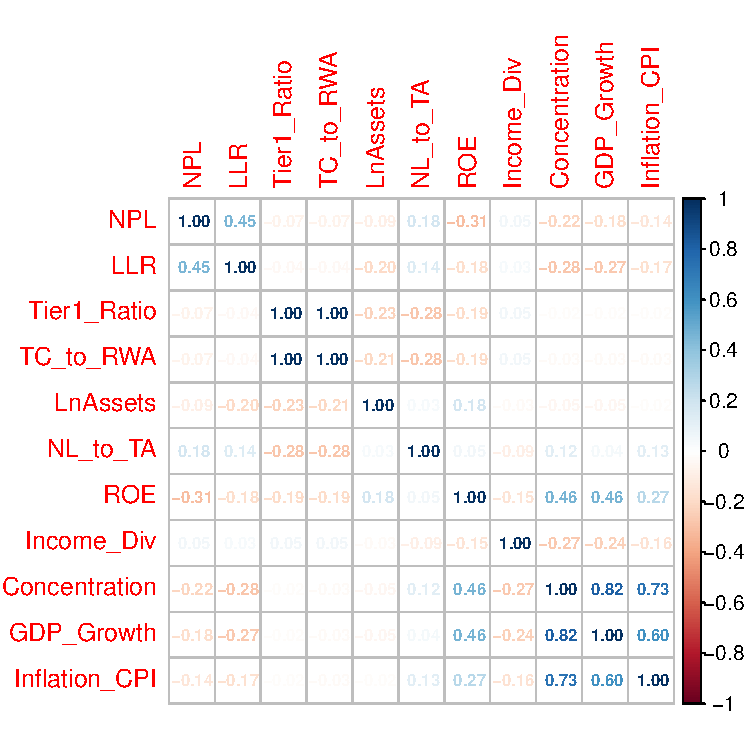
\includegraphics{chapter01-credit_risk_files/figure-pdf/fig-correlation-1.pdf}

}

\caption{\label{fig-correlation}Linear Correlation Matrix}

\end{figure}%

\subsection{Impact on bank credit risk -- Risk-based total capital
ratio}\label{impact-on-bank-credit-risk-risk-based-total-capital-ratio}

\begin{longtable}[]{@{}ccccc@{}}

\caption{\label{tbl-baseline}OLS Baseline Regression}

\tabularnewline

\toprule\noalign{}
\endhead
\bottomrule\noalign{}
\endlastfoot
~ & \multicolumn{2}{c}{%
NPL} & \multicolumn{2}{c@{}}{%
LLR} \\
Predictors & Estimates & CI & Estimates & CI \\
(Intercept) & 3.845 \textsuperscript{***} & 2.727~--~4.962 & 10.797
\textsuperscript{***} & 9.726~--~11.868 \\
TC\_to\_RWA & -0.005 \textsuperscript{***} & -0.007~--~-0.002 & -0.003
\textsuperscript{*} & -0.005~--~-0.000 \\
LnAssets & -0.050 \textsuperscript{**} & -0.086~--~-0.014 & -0.179
\textsuperscript{***} & -0.214~--~-0.144 \\
NL\_to\_TA & 0.023 \textsuperscript{***} & 0.017~--~0.029 & 0.019
\textsuperscript{***} & 0.013~--~0.024 \\
ROE & -0.054 \textsuperscript{***} & -0.065~--~-0.044 & 0.023
\textsuperscript{***} & 0.014~--~0.032 \\
Income\_Div & 0.001 \textsuperscript{} & -0.145~--~0.146 & -0.224
\textsuperscript{**} & -0.363~--~-0.084 \\
Concentration & -0.056 \textsuperscript{***} & -0.087~--~-0.025 & -0.112
\textsuperscript{***} & -0.142~--~-0.083 \\
GDP\_Growth & 0.082 \textsuperscript{} & -0.005~--~0.169 & -0.161
\textsuperscript{***} & -0.245~--~-0.077 \\
Inflation\_CPI & -0.022 \textsuperscript{} & -0.102~--~0.057 & 0.082
\textsuperscript{*} & 0.006~--~0.157 \\
Observations & \multicolumn{2}{l}{%
1649} & \multicolumn{2}{l@{}}{%
1847} \\
R\textsuperscript{2} / R\textsuperscript{2} adjusted &
\multicolumn{2}{l}{%
0.160 / 0.156} & \multicolumn{2}{l@{}}{%
0.177 / 0.174} \\
\multicolumn{5}{@{}r@{}}{%
* p\textless0.05~~~** p\textless0.01~~~*** p\textless0.001} \\

\end{longtable}

Table~\ref{tbl-baseline} reports fixed effect baseline regression
results for the full sample of banks. The columns show the results for
Equation (1). The first two columns use NPL, and columns (3) and (4) use
LLR as the dependent variable. The regressions report negative and
statistically significant relationships between bank credit risk
variables and the risk-based the total capital ratio
(\emph{TC\_to\_RWA}). The results support the hypothesis: higher
regulatory capital requirements are related to lower bank credit risk.

The finding can be explained by the fact that those Chinese banks with
higher level of regulatory capital have higher capability to reduce the
impact of Non-Performing Loans, and thus lower Loan Loss Reserve. Tan
and Floros (2013) find a negative but insignificant relationship between
bank risk and capitalization when Loan Loss Reserve to Gross Loans is
employed as the proxy of risk. Lee et al. (2015) report a significant
negative relationship between bank capital and credit risk (proxied by
NPL ratio). This finding may reveal that the capital adequacy
requirements of Basel III equip commercial banks in China with proper
capital buffers in terms of mitigating credit risk.

Among bank-specific and macroeconomic control variables, we find that
bank size, asset quality, and profitability are the most significant
variables. Bank size has a significant and negative impact on Chinese
banks' credit risk. This result is consistent with findings from some
studies regarding the impact of capital ratios on bank credit risk Bitar
et al. (2018). This finding suggests that large banks are more competent
in dealing with risky loans and or they can spread the risk across a
larger more diverse loan risk profile. Because large banks may benefit
from firm reputation, compared to small banks, and have wide-ranging
access to fixed-income and equity markets to diversify and hedge their
credit risk. There is a significant and negative relationship between
banking industry concentration and individual banks' credit risk. The
total assets of the largest six commercial banks\footnote{The largest
  six commercial banks: Industrial and Commercial Bank of China,
  Agricultural Bank of China, Bank of China, China Construction Bank,
  Bank of Communications, and Postal Savings Bank of China. The first
  four banks are listed as global systemically important banks (G-SIBs)
  in the FSB 2020 G-SIBs list.} account for 41.87\% averagely during
2010-2019, although the industry concentration shows roughly a
year-by-year decrease in the past decade. The first four out of these
six banks are listed as global systemically important banks (G-SIBs) by
Financial Stability Board (FSB) in 2020. In the context of China's
banking industry, these six banks have a better ability to reduce the
pressure in their credit activities, compared with other medium and
smaller-sized banks.

\subsection{Impact on bank credit risk -- Ownership
structure}\label{impact-on-bank-credit-risk-ownership-structure}

\begin{longtable}[]{@{}
  >{\centering\arraybackslash}p{(\columnwidth - 8\tabcolsep) * \real{0.2000}}
  >{\centering\arraybackslash}p{(\columnwidth - 8\tabcolsep) * \real{0.2000}}
  >{\centering\arraybackslash}p{(\columnwidth - 8\tabcolsep) * \real{0.2000}}
  >{\centering\arraybackslash}p{(\columnwidth - 8\tabcolsep) * \real{0.2000}}
  >{\centering\arraybackslash}p{(\columnwidth - 8\tabcolsep) * \real{0.2000}}@{}}

\caption{\label{tbl-ownership}OLS Regression-Ownership Structure}

\tabularnewline

\toprule\noalign{}
\endhead
\bottomrule\noalign{}
\endlastfoot
~ &
\multicolumn{2}{>{\centering\arraybackslash}p{(\columnwidth - 8\tabcolsep) * \real{0.4000} + 2\tabcolsep}}{%
NPL} &
\multicolumn{2}{>{\centering\arraybackslash}p{(\columnwidth - 8\tabcolsep) * \real{0.4000} + 2\tabcolsep}@{}}{%
LLR} \\
Predictors & Estimates & CI & Estimates & CI \\
(Intercept) & 3.271 \textsuperscript{***} & 2.027~--~4.516 & 9.705
\textsuperscript{***} & 8.584~--~10.826 \\
TC to RWA & -0.003 \textsuperscript{*} & -0.005~--~-0.000 & -0.000
\textsuperscript{} & -0.003~--~0.002 \\
LnAssets & -0.075 \textsuperscript{**} & -0.120~--~-0.030 & -0.224
\textsuperscript{***} & -0.265~--~-0.183 \\
NL to TA & 0.019 \textsuperscript{***} & 0.013~--~0.025 & 0.011
\textsuperscript{***} & 0.005~--~0.016 \\
ROE & -0.070 \textsuperscript{***} & -0.081~--~-0.059 & -0.017
\textsuperscript{***} & -0.027~--~-0.007 \\
Income Div & 0.056 \textsuperscript{} & -0.089~--~0.201 & -0.104
\textsuperscript{} & -0.236~--~0.027 \\
Concentration & -0.043 \textsuperscript{**} & -0.074~--~-0.012 & -0.083
\textsuperscript{***} & -0.111~--~-0.055 \\
GDP Growth & 0.079 \textsuperscript{} & -0.007~--~0.165 & -0.139
\textsuperscript{***} & -0.218~--~-0.060 \\
Inflation CPI & -0.020 \textsuperscript{} & -0.098~--~0.058 & 0.068
\textsuperscript{} & -0.003~--~0.138 \\
\begin{minipage}[t]{\linewidth}\raggedright
Ownership {[}Foreign\\
Joint-stock{]}\strut
\end{minipage} & 0.877 \textsuperscript{***} & 0.552~--~1.203 & 1.523
\textsuperscript{***} & 1.260~--~1.787 \\
Ownership {[}Joint-stock{]} & 0.913 \textsuperscript{***} &
0.656~--~1.170 & 1.521 \textsuperscript{***} & 1.333~--~1.708 \\
\begin{minipage}[t]{\linewidth}\raggedright
Ownership {[}Local\\
government-holding{]}\strut
\end{minipage} & 0.938 \textsuperscript{***} & 0.671~--~1.205 & 1.452
\textsuperscript{***} & 1.252~--~1.653 \\
Ownership {[}State-owned{]} & 1.002 \textsuperscript{***} &
0.639~--~1.364 & 1.603 \textsuperscript{***} & 1.303~--~1.903 \\
Observations &
\multicolumn{2}{>{\raggedright\arraybackslash}p{(\columnwidth - 8\tabcolsep) * \real{0.4000} + 2\tabcolsep}}{%
1649} &
\multicolumn{2}{>{\raggedright\arraybackslash}p{(\columnwidth - 8\tabcolsep) * \real{0.4000} + 2\tabcolsep}@{}}{%
1847} \\
R\textsuperscript{2} / R\textsuperscript{2} adjusted &
\multicolumn{2}{>{\raggedright\arraybackslash}p{(\columnwidth - 8\tabcolsep) * \real{0.4000} + 2\tabcolsep}}{%
0.186 / 0.180} &
\multicolumn{2}{>{\raggedright\arraybackslash}p{(\columnwidth - 8\tabcolsep) * \real{0.4000} + 2\tabcolsep}@{}}{%
0.281 / 0.276} \\
\multicolumn{5}{@{}>{\raggedleft\arraybackslash}p{(\columnwidth - 8\tabcolsep) * \real{1.0000} + 8\tabcolsep}@{}}{%
* p\textless0.05~~~** p\textless0.01~~~*** p\textless0.001} \\

\end{longtable}

Table~\ref{tbl-ownership} reports the results of the impact on bank
credit risk by adding banks' ownership structure as a specific control
variable. We find that adding ownership structure does not change the
significant and negative impact of bank size, equity return and industry
concentration on bank credit risk, respectively. However, the
relationship between the capital requirement and Loan Loss Reserve
becomes insignificant, although it remains negative. The relationship
between total regulatory capital and Loan Loss Reserve also remains
negative. The results presented in Table~\ref{tbl-ownership} demonstrate
that ownership structure is positively associated with bank credit risk.
This finding is consistent with the view that shareholders have greater
incentives for risky projects than managers (see John et al., 2008).
This finding also supports the empirical results of Laeven and Levine
(2009) that find a positive association between risk and ownership of a
large owner (10\% or more voting rights).

As discussed in the previous sections, ownership structure is always a
focus of research in terms of China's banking industry. Berger et al.
(2009) study efficiency of Chinese banks from the perspective of
ownership structure and suggest that a minority of foreign ownership
help improve bank efficiency. Pessarossi and Weill (2015) investigate
the effect of capital ratio on Chinese banks' cost efficiency adjusting
for ownership structure. Zhang et al. (2016) compare bank risks between
different ownership structures of Chinese banks. The reason that the
ownership structure becomes of one of the main interest factors in
Chinese banking research could stem from the unique growth path of
China's banking industry and suspicion in Western democracies of latent
state manipulation. The past four decades witnessed dramatic changes and
development in China's banking sector. The three stages of the reform in
China's banking industry achieved the advancement of the legal and
financial infrastructure, as well as the more diversified ownership
structure. By 2010 the four G-SIBs and other 12 commercial banks all
completed IPOs. Private shareholding accounted for 77.7\% in rural
commercial banks. The period after 2010 could be considered not only as
a stage of the financial reform for further progressing and improving,
but also a time to evaluate the effectiveness of the substantial bank
ownership changes. In recent times, as China seeks to decouple its
reserve banking system from the US, there may be important implications
for continued regulatory cooperation in international
banking\footnote{\url{https://rhg.com/research/us-china-decoupling}}.

The results reveal that state-owned banks have higher credit risk
compared to those foreign-owned banks in China's banking industry. This
finding, to some extent, supports the viewpoint that state-owned banks
would be involved in policy-guided credit activities instead of
profit-centered ones (see Pessarossi and Weill, 2015). The social
lending theory of state ownership (see Atkinson and Stiglitz, 1980)
suggests that state-owned enterprises contribute to ``correcting the
`failure' of market economy'' due to imperfect competition, inefficiency
and public good. According to this view, government-owned enterprises
may help improve overall performance of economy (see Stiglitz, 1993). In
China's banking context, the biggest four commercial banks were founded
and conducted a large amount of government lending in the early 1990's,
before national banks and city banks were established. Within a
relatively long period, the state-owned banks (including local
government-holding banks founded later in the end of 1990's) played a
role of `government agencies' to pursue the broader social welfare
objectives rather than profit maximizing; for example, the projects of
the nationwide High-speed Rail network. Since the state-owned banks
target multiple welfare objectives which might not be measurable, the
managers in the state-owned banks have low powered incentives (see
Tirole, 1994). However, this resulted in the significant non-performing
loan levels of `Big Four' banks before China's WTO accession in 2001.

Since 2001, the ownership structure has been dramatically transformed,
due to China's overall industrial reforms and the commitments to the WTO
agreement. The large part of shares directly held by local government
were gradually replaced by mixed ownership enterprises, foreign
investments, and private investors. In terms of the state-owned banks,
direct state intervention was replaced by Central Huijin (a company
representing the state government) along with the establishment of
modern corporate governance system. Why does state ownership still have
relatively higher credit risk? This can be explained by two reasons: (1)
although the direct government shareholding structure changed, business
connection with state-owned enterprises remains due to the long-lasting
business relationship and contracts such as those nationwide
infrastructure projects lasting for decades; (2) the development of
modern corporate governance mechanisms in China's banking industry could
transform government ownership into concentrated ownership, the
ownership similar to the one of large investors with significant control
rights and cash flow rights (see Shleifer and Vishny, 1997). From this
perspective, concentrated ownership puts pressure on management decision
(Shleifer and Vishny, 1997) and bank risk taking incentives (Boyd and
Hakenes, 2008) Almost all state-owned banks are listed banks. With their
significant control rights and cash flow rights, the state (large)
shareholder in these state-owned, listed banks may take excessive risk
by favouring particular clientele such as large conglomerates in
projects with potential of social-benefits rather than those with target
of profit-maximizing. Sapienza (2004) finds that state-owned banks
favour large firms and charge lower interest rates than other types of
banks in Italy. This finding is also consistent with Laeven and Levine
(2009) that report banks with large investors have higher risk.

\subsection{Impact on bank credit risk -- Interaction between regulation
and ownership
structure}\label{impact-on-bank-credit-risk-interaction-between-regulation-and-ownership-structure}

\begin{longtable}[]{@{}
  >{\centering\arraybackslash}p{(\columnwidth - 8\tabcolsep) * \real{0.2000}}
  >{\centering\arraybackslash}p{(\columnwidth - 8\tabcolsep) * \real{0.2000}}
  >{\centering\arraybackslash}p{(\columnwidth - 8\tabcolsep) * \real{0.2000}}
  >{\centering\arraybackslash}p{(\columnwidth - 8\tabcolsep) * \real{0.2000}}
  >{\centering\arraybackslash}p{(\columnwidth - 8\tabcolsep) * \real{0.2000}}@{}}

\caption{\label{tbl-interaction}Regression with Interaction between
Ownership and Capital Regulation}

\tabularnewline

\toprule\noalign{}
\endhead
\bottomrule\noalign{}
\endlastfoot
~ &
\multicolumn{2}{>{\centering\arraybackslash}p{(\columnwidth - 8\tabcolsep) * \real{0.4000} + 2\tabcolsep}}{%
NPL} &
\multicolumn{2}{>{\centering\arraybackslash}p{(\columnwidth - 8\tabcolsep) * \real{0.4000} + 2\tabcolsep}@{}}{%
LLR} \\
Predictors & Estimates & CI & Estimates & CI \\
(Intercept) & 3.636 \textsuperscript{***} & 2.404~--~4.867 & 9.766
\textsuperscript{***} & 8.643~--~10.888 \\
TC to RWA & -0.002 \textsuperscript{} & -0.005~--~0.000 & -0.000
\textsuperscript{} & -0.002~--~0.002 \\
LnAssets & -0.100 \textsuperscript{***} & -0.145~--~-0.055 & -0.229
\textsuperscript{***} & -0.271~--~-0.187 \\
NL to TA & 0.019 \textsuperscript{***} & 0.014~--~0.025 & 0.010
\textsuperscript{***} & 0.005~--~0.015 \\
ROE & -0.071 \textsuperscript{***} & -0.082~--~-0.060 & -0.019
\textsuperscript{***} & -0.029~--~-0.009 \\
Income Div & 0.024 \textsuperscript{} & -0.120~--~0.168 & -0.091
\textsuperscript{} & -0.222~--~0.041 \\
Concentration & -0.042 \textsuperscript{**} & -0.073~--~-0.012 & -0.082
\textsuperscript{***} & -0.110~--~-0.054 \\
GDP Growth & 0.063 \textsuperscript{} & -0.023~--~0.148 & -0.137
\textsuperscript{***} & -0.215~--~-0.058 \\
Inflation CPI & 0.001 \textsuperscript{} & -0.076~--~0.078 & 0.059
\textsuperscript{} & -0.011~--~0.130 \\
\begin{minipage}[t]{\linewidth}\raggedright
Ownership {[}Foreign\\
Joint-stock{]}\strut
\end{minipage} & 1.245 \textsuperscript{} & -0.428~--~2.918 & 2.125
\textsuperscript{***} & 1.738~--~2.512 \\
Ownership {[}Joint-stock{]} & 2.269 \textsuperscript{***} &
1.787~--~2.752 & 1.312 \textsuperscript{***} & 0.882~--~1.743 \\
\begin{minipage}[t]{\linewidth}\raggedright
Ownership {[}Local\\
government-holding{]}\strut
\end{minipage} & 1.988 \textsuperscript{***} & 1.266~--~2.709 & 0.908
\textsuperscript{**} & 0.242~--~1.573 \\
Ownership {[}State-owned{]} & 2.314 \textsuperscript{***} &
0.984~--~3.644 & 1.743 \textsuperscript{**} & 0.456~--~3.029 \\
\begin{minipage}[t]{\linewidth}\raggedright
TC to RWA × Ownership\\
{[}Foreign Joint-stock{]}\strut
\end{minipage} & -0.022 \textsuperscript{} & -0.150~--~0.105 & -0.039
\textsuperscript{***} & -0.057~--~-0.021 \\
\begin{minipage}[t]{\linewidth}\raggedright
TC to RWA × Ownership\\
{[}Joint-stock{]}\strut
\end{minipage} & -0.097 \textsuperscript{***} & -0.126~--~-0.067 & 0.018
\textsuperscript{} & -0.010~--~0.046 \\
\begin{minipage}[t]{\linewidth}\raggedright
TC to RWA × Ownership\\
{[}Local\\
government-holding{]}\strut
\end{minipage} & -0.076 \textsuperscript{**} & -0.126~--~-0.025 & 0.044
\textsuperscript{} & -0.004~--~0.092 \\
\begin{minipage}[t]{\linewidth}\raggedright
TC to RWA × Ownership\\
{[}State-owned{]}\strut
\end{minipage} & -0.091 \textsuperscript{} & -0.192~--~0.009 & -0.007
\textsuperscript{} & -0.104~--~0.091 \\
Observations &
\multicolumn{2}{>{\raggedright\arraybackslash}p{(\columnwidth - 8\tabcolsep) * \real{0.4000} + 2\tabcolsep}}{%
1649} &
\multicolumn{2}{>{\raggedright\arraybackslash}p{(\columnwidth - 8\tabcolsep) * \real{0.4000} + 2\tabcolsep}@{}}{%
1847} \\
R\textsuperscript{2} / R\textsuperscript{2} adjusted &
\multicolumn{2}{>{\raggedright\arraybackslash}p{(\columnwidth - 8\tabcolsep) * \real{0.4000} + 2\tabcolsep}}{%
0.211 / 0.204} &
\multicolumn{2}{>{\raggedright\arraybackslash}p{(\columnwidth - 8\tabcolsep) * \real{0.4000} + 2\tabcolsep}@{}}{%
0.290 / 0.284} \\
\multicolumn{5}{@{}>{\raggedleft\arraybackslash}p{(\columnwidth - 8\tabcolsep) * \real{1.0000} + 8\tabcolsep}@{}}{%
* p\textless0.05~~~** p\textless0.01~~~*** p\textless0.001} \\

\end{longtable}

Table~\ref{tbl-interaction} presents results pertaining to the
interactive associations among ownership structure, the regulatory
capital, and bank credit risk. Some studies suggest that the
relationship between risk and ownership structure is closely associated
with national regulation because regulation influences both bank owners'
and bank managers' incentives of risk-taking and risk-shifting (John et
al., 2008, 2000). Laeven and Levine (2009) examine the interactions
between ownership structure and national regulatory requirements and
stringency, and find the relationship between risk and regulation
stringency depends on ownership structure. Berger and Bouwman (2013)
state that capital requirements have different impact on bank
performance based on different bank size. Here we include the
interaction term of the capital adequacy variable with different
ownership structure variables. The capital adequacy variable becomes
statistically insignificant under the circumstance of the interactive
association between the capital ratio and ownership structure, although
is still negatively related to bank credit risk.

After adding the interactive term, the coefficients of the ownership
structure variables are positive and significant in
Table~\ref{tbl-interaction}. This finding may partially support the
theories arguing that bank owners may choose to increase portfolio risk
when facing more stringent capital requirements, in order to compensate
their potential loss of expected utility (Buser et al., 1981; Koehn and
Santomero, 1980). Table~\ref{tbl-interaction} shows that local
government-holding banks have a relatively lower positive coefficient
than other types of banks, indicating that local government-holding
banks may have lower incentives to reshuffle risk when facing higher
capital adequacy regulation.

Most of the interactive coefficient estimates in the NPL regression show
negative relation to bank credit risk-taking. By including the
interaction term between capital and ownership structure, the results
reveal that the effect of capital regulation of mitigating bank credit
risk and enhance bank stability, to some extent, depends on ownership
structure. Among these terms, the joint-stock and local
government-holding terms enter the most significantly. This shows that
the impact on bank credit risk of the total regulatory capital ratio can
be magnified when banks are not dominated by a single large
owner\footnote{In our sample, the direct(indirect) shares of local
  government-holding banks held by government or its agencies are over
  10\%. However, the local government-holding banks don't have dominant
  direct(indirect) government shareholders (50\% more voting rights). In
  fact, most of these banks are widely held and have mixed-ownership
  shareholders.}.

The interaction between regulatory capital and the state ownership also
acts effectively in reducing bank risk-taking. Laeven and Levine (2009)
argue that regulations affecting risk-taking incentives of banks with
powerful owners and the ones widely held may be in different ways. The
finding may be interpreted in that the interaction between capital
regulations and the incentives of joint-stock shareholders is more
significant than powerful shareholders, because shareholders of
joint-stock banks may have different risk-taking incentives from the
influential state-shareholders. The joint-stock banks and those local
government-holding banks may be more sensitive to capital regulation.
This result, to some extent, collaborates with the estimates of the
coefficients of ownership structure.

\section{Conclusion}\label{conclusion-1}

This paper aims to analyze the impact of capital regulation on Chinese
banks' credit risk-taking following the 2007-2009 GFC and to assess the
impact of capital regulation on credit risk-taking by incorporating the
interaction between capital regulation and ownership structure. We focus
on risk-based capital regulation from the Basel III framework that
affects Chinese commercial banks over the period 2010-2019. This period
coincides with the fourth stage of China's financial reform and the
implementation of Basel III framework in China. Financial theories,
supported by empirical studies, suggest that the impact of bank
regulation on bank risk-taking varies due to different ownership
structure (Laeven and Levine, 2009). Therefore, this study provides
implications for regulatory strategies and the stability of China's
banking system.

We find that Basel III risk-based capital regulation has a negative
impact on bank credit risk-taking. This finding implies that
implementation of Basel III capital regulation has strengthened
financial stability. We compare the credit risk-taking level of
different ownership structure in China's commercial banks and find that
state-owned banks have higher credit risk-taking than any other
ownership structure in China's banking industry. This finding is
consistent with the social view of the state ownership theory, as well
as the theory predicting that powerful shareholders have stronger
incentives to take risks due to the transformation of ownership
structure during China's financial reform.

Furthermore, we find that the impact of capital regulation on credit
risk-taking is influenced by ownership structure. The same bank
regulations have different effects on credit risk-taking because of the
interaction between bank regulation and ownership structure. Thus, this
paper provides strategic implication for regulatory authorities making
regulatory decisions to take into account bank ownership structure.

\bookmarksetup{startatroot}

\chapter{Does stringent capital regulation affect persistent or
transient Chinese bank efficiency-A four-component model
analysis}\label{does-stringent-capital-regulation-affect-persistent-or-transient-chinese-bank-efficiency-a-four-component-model-analysis}

\section{Introduction}\label{introduction-2}

Since the first Basel Accord (Basel I) in 1988, followed by Basel II in
2004 and Basel III in 2010, capital regulation has been put at the front
and center to regulate banks' behavior and maintain well-functioning
banking systems. Over the last few decades, regulatory capital
requirements have been refined and broadened to cover increasing types
of risk and keep up with the growing complexity of banking. The
2007-2009 global financial crisis uncovers that capital regulations
which were implemented before the crisis were inadequate to prevent a
financial panic and cover unexpected losses. After the crisis, the Basel
Committee on Banking Regulation and Supervision (BCBS) developed a
consolidated framework (Basel III) for more stringent capital adequacy
regulations and liquidity assessment, in recognition of the need for
banks to be subject to more stringent capital regulations. Following the
goals set by the BCBS, member countries including China have established
legislation and regulatory frameworks.

China's banking sector plays an essential role in the country's economic
development. China's banking sector has started a fundamental reform
since 1978, as an integrate part of China's overall economic reform.
Since 2001 when China got accession to the World Trade Organization
(WTO), the reform of China's banking system has stepped up its pace and
the whole banking sector has been dramatically reshaped. The reform has
transformed Chinese banks into market-oriented enterprises, changed
ownership structure of Chinese banks, established modern corporate
governance mechanisms, and introduced legislation and regulatory
framework. Since 2010, improvements and refinements have happened in
China's banking sector as an advanced stage of the reform. China's
financial authority fully accepted the Basel III framework and started
the implementation in 2013.

While regulatory consensus has been reached that more stringent capital
requirements maintain an essential role in the Basel III framework,
there has been less agreement among academics on debates regarding
whether capital regulation influences financial stability through the
impact it has on bank efficiency. From the perspective of the role of
government, ``the public interest'' approach holds that bank regulation
enhances social welfare therefore improve efficiency (see Barth et al.,
2005). The conflicting approach ``the private interest'' view argues
that regulation only benefits political patronage (see Stigler, 1971)
and impedes bank efficiency. From the perspective of corporate
governance, literature provides two main hypotheses to explain the
relationship between capital and efficiency. The conflict between
shareholders and creditors (``asset substitution'' hypothesis, see Smith
and Warner, 1979) favors that high capital reserve leads to better bank
performance. In contrast, the conflict between shareholders and managers
(``control'' hypothesis, see Jensen, 1986) asserts that high regulatory
capital holding harms bank efficiency.

In this paper, we evaluate the impact of the capital regulation on
bank's cost efficiency in China's banking industry. Given these opposing
views and previous empirical studies with conflicting results based on
various theoretical models, we believe that our empirical research could
be important for policy decision making.

A second question that we address in this paper is relationship between
ownership and bank efficiency. China's financial reform has dramatically
transformed bank ownership which could be important implication for bank
efficiency (Berger et al., 2009). Along with embracing privatization and
establishment modern corporate governance, China's financial reform has
evolved state ownership into a large-investor shareholding type with
significant cash flow rights. Theory offers two opposing views on the
nexus between state ownership and bank efficiency: the public view holds
that state ownership improves bank efficiency (see Atkinson and
Stiglitz, 1980; Stiglitz, 1993); while the political view claims that
state ownership jeopardizes bank performance (see Shleifer and Vishny,
1997, 1994). Therefore, these theoretical keystones provide the
foundation for us to examine bank efficiency associated with ownership
structure of Chinese banks.

Our empirical research provides evidence using a four-component panel
stochastic frontier cost model on an unbalanced panel of 233 China's
commercial banks over the period 2010-2020. To perform our analysis, we
hand collect the ownership structure information of these 233 China's
commercial banks and categorize them into 5 ownership identities:
State-owned (Big Six and other than Big Six), Local government-holding,
Joint-stock, foreign joint-stock, and Foreign-owned banks, referencing
the definitions by China Banking and Insurance Regulatory
Commission(CBIRC) (see Table~\ref{tbl-ownership}). We employ the total
regulatory capital ratio (TC/RWA) defined by the Basel III to
investigate impact of capital regulation on bank cost efficiency and the
relationship between ownership and bank cost efficiency.

The key findings are as follows: first, we do not find statistically
significant relation between the regulatory capital requirements and
bank persistent(time-invariant) cost efficiency, but a negative
associtation between Basel III regulatory capital and
transient(time-varying) efficiency. This result supports the results by
Barth et al. (2004), Lee and Chih (2013), Djalilov and Piesse (2019) and
Lešanovská and Weill (2016), but differ from other previous studies.

Second, the estimate of state ownership shows statistically significant
relation with bank cost efficiency. The results provide that state-owned
banks have higher transient efficiency and much lower persistent
efficiency compared with other ownership types. This finding collaborate
the findings by Fungáčová et al. (2020). By decomposing the overall
efficiency into transient and persistent efficiency, we also provide
explanations for different ownership types with similar efficiency
patterns.

This paper contributes to the literature in several ways. First, this
study assesses the impact of risk-based capital regulation on Chinese
banks' cost efficiency following the global financial crisis, using the
definition of capital from Basel III framework. The BCBS first released
Basel III framework in 2010. The Chair of the BCBS addressed that
evaluating the regulation effects is part of the BCBS post-crisis reform
in the current macroeconomic environment. In addition, China's banking
industry achieved extensive transformation before 2010 and the Chinese
case provides uniqueness in terms of ownership structure.

Second, despite the extensive literature on bank efficiency, the
literature falls short of explaining low efficiency. This gap may be due
to limitation on methodologies. In this paper, we apply the most recent
four-component SFA cost model developed by Colombi et al. (2011),
Colombi et al. (2014), Filippini and Greene (2016), and Kumbhakar et al.
(2015). It enables us to decompose the overall efficiency into transient
and persistent components. The transient inefficiency is time-varying
and may stem from short-run moral hazard such as non-optimal resource
allocation and changes to adapt new economic environment. The persistent
inefficiency may be due to regulations, infrastructure, investments or
lasting management habits (of wasting inputs) such as poor organization
or private incentives of preventing cost minimization. By using the new
model we disentangle transient and persistent (in)efficiencies and
provide important empirical evidence for efficiency literature.

Third, we use a bespoke dataset of 233 Chinese commercial banks over a
relatively long period (2010-2020) to study China's banking sector.
These 233 banks account for over 91\% of China's banking sector in terms
of total assets. Apart from employing the data provided by the SNL
database, we hand collected the missing values of the data set from the
original annual reports of individual bank, which makes our data set
extremely comprehensive.

The remainders of this paper proceeds as follows. Section II reviews the
related literature, as well as information of China's financial reform
and the evolution of ownership structure of commercial banks in China.
Section III presents the data set and the empirical model specification.
The empirical results are presented in section IV. And section V
concludes.

\section{Literature review}\label{literature-review}

In this section, we review the theoretical and empirical literature
pertaining to the effect of capital regulation on bank efficiency, and
provide information of China's financial reform as well as the evolution
of ownership structure in China's banking industry.

\subsection{Two approaches to bank
regulation}\label{two-approaches-to-bank-regulation}

Regarding the role of government in regulating economic activities,
there are two main approaches to bank regulation and supervision: the
public interest view and the private interest view. The public interest
approach to bank regulation and supervision emphasizes that governments
regulate banks thereby safeguarding the interest of the public and
enhancing social welfare (Barth et al., 2005). Cannan and Pigou (1921)
and Atkinson and Stiglitz (1980) are in favor of government intervention
in bank regulating and supervising which can be traced back to welfare
economics. They argue that there are important reasons for government
intervention including failure of perfect competition, external shocks,
public goods, among others. According to the public interest view, bank
regulation may reduce unnecessary risk in lending and boost competition,
leading to great bank efficiency(Barth et al., 2005).

ON the other hand, the private interest view (the ``capture'' theory,
see Jensen (1986)) argues that regulation only benefits specific groups
because it is sabotaged by the political process. Applied to banking
industry, bank regulations are captured to enhance the well-being of
bankers and closely connected to the political parties. The private
interest view can be considered to share the similar viewpoint with the
political view regarding state ownership in the economy. Governments
have agendas which are other than social welfare and dominated by their
own political interests. Governments use their control only to transfer
wealth to their supporters, leading low efficiency of state firms
(Shleifer, 1998; Shleifer and Vishny, 1997). Accordingly, the private
view criticizes that stringent bank regulations may reduce bank
efficiency and exacerbate corruption in lending. The private interest
view also advocates extensive reliance on market discipline, voluntary
disclosure and private sector initiatives (Shleifer, 2005).

Given that the theories provide conflicting prediction about the impact
of bank regulation policies on efficiency, the empirical literature
gives mixed findings related to the above theoretical models. Barth et
al. (2004) investigate the relationship between regulatory and
supervisory practices and bank performance and stability of banking
sector using the World Bank survey data for a sample of 107 countries.
The empirical results suggest that there is no statistically significant
relation between official supervisory power and bank performance.
However, they find private monitoring is positively related to bank
development and negatively associated with overhead costs. They also
report that countries facilitating strong market discipline system have
better preformed banks. Beck et al. (2006) examine the impact of bank
supervision on lending across 37 countries employing firm data of the
World Business Environment Survey (WBES) and the bank supervisory data
of Barth et al. (2004). The results suggest that strengthening official
supervisory power increases the corruption in lending which may result
in lower efficient credit allocation. The results also advocate that
supervisory policies enforcing accurate information disclosure
facilitate integrity in lending with implication of higher efficient
credit allocation. Being consistent with the public interest view,
Pasiouras (2008) finds powerful supervisory agencies have positive
impact on banks' technical efficiency in several cases of Tobit
regression. Pasiouras et al. (2009) also report that banks' cost and
profit efficiency are influenced positively by strong official
supervisory power. Nevertheless, Pasiouras (2008) and Pasiouras et al.
(2009) also find empirical evidence supporting the view that creating
and strengthening market discipline mechanism are associated with higher
bank efficiency. Barth et al. (2013) study the impact of bank regulation
and supervision on bank efficiency using the previous bank supervisory
database(Barth et al., 2008, 2005, 2004) and firm-level data for a
sample of 72 countries over the period 1999-2007. They find that
enhancing official supervisory power has positive impact on bank
efficiency in those countries where supervisory authorities are more
independent. The results also suggest that market-based monitoring with
more financial transparency is positively related to bank efficiency.

Regionally, Chortareas et al. (2012) examine the relationship between
the supervisory policies and bank efficiency employing a sample of banks
in 22 European Union countries. They find that both strengthening
official supervisory powers and private sector monitoring can improve
bank efficiency levels. Lee and Chih (2013) study how bank regulation
affect banks' cost efficiency and risk in China. They report empirical
results that different regulatory ratios have different impact on
efficiency of big banks and small banks. They also suggest that
policymakers in China face a trade-off between risk and efficiency.
Haque and Brown (2017) examine the effects of bank regulation and
ownership on bank efficiency in Middle East and North Africa (MENA)
region and find evidence supporting the public view that official power
has positive impact on cost efficiency. Djalilov and Piesse (2019)
investigate the relationship between bank regulation and bank efficiency
in 21 transition countries for the period 2002-2014 and find that
neither official supervisory power nor market discipline have
statistically significant effects on bank efficiency.

\subsection{Bank Capital and
Efficiency}\label{bank-capital-and-efficiency}

Capital adequacy requirements, as one of the main regulatory tools, are
of the essence of the Basel III framework. Regulatory capital provides a
potential buffer in absorbing liquidity and economic shocks during the
time of stress and thereby improve stability of the financial system
(Anginer et al., 2021; Repullo, 2004). Based on the public interest
view, a powerful regulatory agency can improve bank operations by
requiring higher regulatory capital which aligns the incentives of bank
owners and creditors (Barth et al., 2013, 2005). In contrast, the
private interest approach holds that strong official regulatory agencies
cannot rectify market failures. Rather, the potential benefit from
higher capital adequacy requirements might be offset by increased
regulatory costs including a higher entry barrier and a greater
government rent (Barth et al., 2013, 2005).

Besides the above two approaches to bank regulation and supervision, the
theory literature provides the theories of agency, information
asymmetry, and capital structure to explain the relationship between
bank capital and efficiency. Based on agency theory and information
asymmetry, Jensen and Meckling (1976) argue that asymmetric information
problems may create the conflict between shareholders and creditors.
This may lead to a moral hazard opportunity for shareholders to shift
wealth from creditors to themselves. For example, shareholders may
invest in high-risk assets to substitute lower/safer ones (``asset
substitution,'' see Smith and Warner, 1979), which increases the risks
faced by creditors whereas shareholders are protected by the limited
liability condition. Shareholders may also have the incentives to reject
a project or lack motivation to fund investments which have postie net
present values if the benefits would accrue to creditors (Myers, 1977).
This may cause creditors to suffer opportunity loss. According to these
arguments, higher regulatory capital holding can curtail the
shareholders incentives in risk-taking and risk-shifting, which may
result in more prudent lending and better bank performance (Berger et
al., 1995; Keeley and Furlong, 1990). These arguments show that
incentive effects are consistent with the theoretical grounds of the
public interest view mentioned in Barth et al. (2005). In fact, the
risk-shifting incentive and potential external shocks have been strongly
justified bank capital regulation (Santos, 2001).

However, agency theory also analyzes the conflict between shareholders
and managers arising from managers' control over free cash flows
(``control hypothesis,'' see Jensen, 1986). Managers, with divergent
interest from shareholders, have discretion over how to use the future
cash flows. Managers may lower their effort or waste resources rather
than maximize the firm value. By issuing debt, managers are bonding
themselves to act in the interest of shareholders (Grossman and Hart,
1982). Because managers are held to promise to repay the interests,
which reduces the free cash flow available to management's control
(Jensen, 1986); and the potential threat from bankruptcy may effectively
motivate management to improve the firm's efficiency to avoid personal
costs due to bankruptcy (Grossman and Hart, 1982; Jensen, 1986). Based
on these arguments, higher regulatory capital holding can impede bank
efficiency, as it may exacerbate the conflict between shareholders and
management.

Most of the aforementioned empirical research regarding the impact of
bank regulation and supervision on bank performance report that
stringent capital regulation improve bank performance. Barth et al.
(2004) state that capital stringency may prevent non-performing loans.
Barth et al. (2013) find more stringent capital regulation is positively
associated with bank efficiency. Empirical results provide evidence that
the adoption of stringent capital adequacy standards has an positive
impact on technical efficiency (Pasiouras, 2008) and cost efficiency
(Pasiouras et al., 2009), but a negative impact on profit efficiency
(Pasiouras et al., 2009). Similarly, Chortareas et al. (2012) and Haque
and Brown (2017) also report that strict capital requirements increase
bank efficiency in EU and MENA countries, respectively. However, capital
regulation (regulatory ratio and stringency) does not appear to have a
significant effect on bank efficiency in China (Lee and Chih, 2013) and
transition countries (Djalilov and Piesse, 2019), respectively. In
addition to the above research, Lešanovská and Weill (2016) analyze the
relation between regulatory capital and bank efficiency in Czech's
banking industry and find no relation. Bitar et al. (2018) investigate
the effect of capital ratios on bank risk, efficiency and profitability
in 39 OECD countries and they state that risk-based capital ratio
improve banks' efficiency and profitability.

Although there is a growing empirical literature concerning bank
efficiency in China's banking industry, the research focusing on the
impact of regulatory capital and bank efficiency is still sparse. Most
research papers concentrate on investigating Chinese banks' efficiency
of different ownership types and sizes (Berger et al., 2009; for
example, Fu and Heffernan, 2007; Huang et al., 2017). Tan and Floros
(2013) assess the relationship between bank capital, risk and efficiency
in China's banking industry using non-risk based capital (equity to
total assets ratio) and the empirical results show that bank capital
enters with a positive but not statistically significant coefficient.
Pessarossi and Weill (2015) study the effect of capital requirements on
cost efficiency of Chinese banks over 2004-2009 and they find that
capital adequacy requirements have a positive effect on cost efficiency.

\subsection{Ownership Structure and bank
efficiency}\label{ownership-structure-and-bank-efficiency}

The theory of ownership stems from the pioneering work of the property
rights theory by Coase (1937), Alchian (1965), Demsetz (1966), and
Alchian and Demsetz (1972); has been extended by Grossman and Hart
(1986) and Hart and Moore (1990), and integrated with the agency theory
by Jensen and Meckling (1976), Fama (1980), and Fama and Jensen (1983).
The property rights theory defines ownership as residual right to income
(Alchian and Demsetz, 1972) and residual right to control (Hart and
Moore, 1990); and states that the owners' property rights have been
attenuated by managers' diverting the firm's resources to their own ends
(Furubotn and Pejovich, 1972). The property rights theory allows the
prediction of behavioral consequences of individuals in the contractual
relations (De Alessi, 1980). Therefore, according to the theory
literature, the issue of ownership and efficiency should be considered
in the context of principal-agent framework and public choice theory
(Altunbas et al., 2001). In the following subsections, we review the
theoretical and empirical literature of ownership from two dimensions:
the degree of ownership concentration (shareholder rights) and the
nature of the shareholders (see Shleifer and Vishny, 1997).

\subsubsection{The degree of ownership
concentration}\label{the-degree-of-ownership-concentration}

The separation of ownership and control in modern corporations,
emphasized by Berle and Means (1932), retains a central position in the
literature of the theory of the firm. From the agency perspective,
shareholder rights and ownership concentration are two common approaches
to influence managerial behavior and thereby impact corporate
performance. It is often believed that the diffused ownership would
increase the power of managers and reduce their dependence on the owners
(Berle and Means, 1932). Alchian and Demsetz (1972) argue that, in a
corporation with dispersion of shareholding, control may be facilitated
by turning shareholders' votes into voting blocs, which strengthens
shareholders' power. Amihud and Lev (1981) and Hirshleifer and Thakor
(1992) argue that better investor protection (shareholder rights)
constrain managers' conservative (sub-optimal) risk-taking choices and
may lead to the enhanced firm value. John et al. (2008) conduct a
cross-country study and support this view. They find the positive
relationship between investor protection and firm growth rates. However,
Burkart et al. (2003) present a model arguing that great protection of
shareholder rights reduces the need for dominant shareholders which may
prevent managers' shirking behavior (Shleifer and Vishny, 1986).
Therefore, dispersed shareholding with unrestricted salability may keep
a long-lived management team (Alchian and Demsetz, 1972), and may result
in greater managerial discretion in forgoing value-enhancing investment
projects (Bebchuk, 1999; Burkart et al., 2003).

Voting blocs are a transient reformation of the ownership structure,
converting the diffused ownership into decisive power (Alchian and
Demsetz, 1972) which is one of the characteristics of large
shareholders. Ownership concentration, or large shareholders, is defined
as shareholders having concentrated control rights with significant cash
flow rights (Shleifer and Vishny, 1997). The model presented by Shleifer
and Vishny (1986) to estimate the value of ownership concentration. They
propose that a presence of a large shareholder may lead to
value-increasing takeovers. However, Grossman and Hart (1988) argue that
large shareholders might try to maximize their private benefit at the
expense of other small shareholders if their high control rights are not
associated with high cash flow rights. The model employed by Grossman
and Hart (1988) shows that this happens if there is a substantial
departure from one share-one vote structure. Demsetz and Lehn (1985)
find no linear relationship between ownership concentration and firm
profit rate. Morck et al. (1988) only get significant statistical result
of profit rates rising in the range of ownership between 0 to 5\%. Based
on their finding, as ownership concentration increases beyond a certain
point, large shareholders expropriate the firm resource to generate
private benefits of control and dampen the interests of other investors
and the firm.

\subsubsection{State ownership}\label{state-ownership-1}

From the perspective of corporate governance, state firms are defined as
being ``controlled by the public; and the de facto control rights
usually belong to bureaucrat shareholders with highly concentrated
control rights and no significant cash flow rights'' (Shleifer and
Vishny, 1997). Based on this definition, state shareholders can be
considered as a special form of the large shareholders with highly
concentrated control rights and lack of cash flow rights.

The property rights theory suggests that the difference between public
ownership and private ownership is that public ownership can not be
transferred; and public ownership arrangements have higher costs (lower
efficiency) compared to private property agencies (Alchian, 1965). De
Alessi (1974) states that due to the inability of transferring his
share, the owners of government firms have lower incentives to monitor
managerial behavior. This may imply that a greater attenuation in
owners' rights in government (political) firms, which may lead to less
efficient operations, compared to private firms (De Alessi, 1974).

Associated with the theorem of welfare economics and the property rights
theory, there are two alternative views of government participation in
financial markets: the social view and the political view. The social
view suggests that state ownership is a form of government intervention
which addresses to market failures and improves market functions and
economic performance (Atkinson and Stiglitz, 1980; Stiglitz, 1993).
According to this view, state-owned banks may finance those projects
which might not be profitable but might have high value of social
welfare. Therefore, state-owned banks may have poorer performance in
profitability along with higher default risk compared to their
counterparties in the private sector. In contrast, the political view
claims that state ownership creates sources of political benefits for
politicians rather than social welfare. For example, excessive
employment of state firms only benefits those who support government
politically (Shleifer and Vishny, 1994). According to the political
view, state-owned firms are inefficient because the state shareholders,
with highly concentrated control rights and no cash flow rights, only
maximize their political goals which may jeopardize social welfare
(Shleifer and Vishny, 1997).

A growing literature has examined the impact of state ownership of
banks, from both the macroeconomic angle and the perspective of
individual banks, on economic growth and bank performance. Andrianova et
al. (2012) find that government-owned banks have higher growth rates and
contribute to countries' long-run economic growth. However, La Porta et
al. (2002) find that higher government ownership is related to lower
economic growth. Beck and Levine (2002) find no supporting evidence for
either the social view or the political view. Employing a data set of
banks in 74 countries, Iannotta et al. (2007) argue that state ownership
intensifies bank concentration and exacerbate financing obstacles.
Berger et al. (2005) and Iannotta et al. (2007) find that state-owned
banks have lower profitability and poor long-term performance, compared
to private-owned banks.

As part of the results of the financial reform in China, the evolved
ownership structure of banks in China has attracted academic attention
after China's accession to the WTO in 2001. Studies focusing on bank
efficiency report that state-owned banks exhibit lower efficiency
compare to joint-stock banks and foreign banks (Berger et al., 2009;
Shleifer, 2005). Tan and Floros (2013) argue that state-owned banks have
higher volume of non-performing loans and lower profitability. Zhu and
Yang (2016) report that state-owned banks take higher risk than foreign
banks in China. Using the four-component efficiency model (see Tsionas
and Kumbhakar, 2014), Fungáčová et al. (2020) analyze the overall
efficiency of Chinese banks and find state-owned banks (the Big Five)
suffer low efficiency because of the low persistent efficiency.

\subsubsection{The evolution of ownership structure of commercial banks
in
China}\label{the-evolution-of-ownership-structure-of-commercial-banks-in-china-1}

The dramatic changes regarding the ownership structure of commercial
banks in China are the essential part of every stage in China's
financial reform. The four largest state-owned banks \footnote{They are
  the ``Big Four'': Bank of China, China Construction Bank, Agricultural
  Bank of China, and Industrial and Commercial Bank of China.} were
founded during the first stage of the financial reform (1978-early
1990s), alongside with other national banks \footnote{National banks:
  commercial banks which operate nationwide}. These large banks, at this
stage, were owned by Finance Ministry and state-owned enterprises. The
lower level of financial institutions, known as city credit
cooperatives, were controlled by local Bureau of Finance when
established. Foreign banks were operating in Special Economic Zones
\footnote{Special Economic Zones: a form of Free Ports in China where
  companies may benefit from tariff allowances and exemption. Chinese
  government designated the first four Special Economic Zones --
  Shenzhen, Xiamen, Shantou, and Hainan Province -- in order to
  encourage foreign investments and improve economy and technology by
  the end of 1980's. More details may be found
  \href{http://www.npc.gov.cn/npc/c9757/200904/8e461e2ba405480697185186122812d4.shtml}{here}}
(Berger et al., 2009).\\
During the second stage (early 1990s-2001), most `policy-lending'
business of the four largest state-owned banks was released to three
policy banks founded during this period. Private enterprises and
individuals began entering different levels of financial institutions as
shareholders. Local Bureau of Finance began to exit city banks by
transferring their shareholding to local business enterprises.\\
The biggest change to the ownership structure happened at the third
stage of the financial reform (2001-2010). An investment enterprise ,
Central Huijin Investment Ltd.~(hereafter CH), was established by the
state government acting as a designated shareholder of those state-owned
banks, in order to fulfill the corporate governance requirements set by
laws and regulations. Direct government shareholding has sharply
decreased due to the share transfer to CH and state-owned banks going
public. Foreign financial institutions such as RBS Group and Bank of
America invested in all levels of Chinese banks including state-owned
banks, national banks and city banks, as strategic investors. The
majority of state-owned banks and several city banks went public at this
stage, introducing more diversified shareholders. After 2010, more
detailed improvements happened regarding ownership structure.
Private-owned banks were established. Local government shareholders
become minority shareholders in city banks. Over 50\% of shareholding in
city banks and over 87\% of shareholding in rural commercial banks are
private enterprises by 2017. In total 57 commercial banks are listed by
2020.

After the financial reform, both of shareholding by the state government
and local governments in commercial banks have decreased. Different from
that state-owned banks have Finance Ministry or CH as their controlling
shareholder; ownership structure of local government-holding banks
evolved to government-private ``Mixed'' ownership. In these banks, local
Bureau of Finance is not the controlling shareholder. Local
government-holding banks usually are medium sized banks and provide
financial services in cities and nearby areas.

\section{Data and methodology}\label{data-and-methodology}

\subsection{Data}\label{data-1}

Our sample is an unbalanced panel composed of financial and ownership
data of 233 Chinese banks during the period of 2010-2020, giving in
total 2574 observations. Our data includes all major commercial banks
and covers over 91\% of the Chinese commercial banks in terms of the
total assets. The composition of the sample banks and the information of
their ownership structure are listed in Table~\ref{tbl-ownership}.

We use the SNL database (provided by S\&P Global Market Intelligence) as
our main data source. The data is expressed in real (2010) term using
China GDP deflator. Whenever the SNL does not provide enough information
or has doubtful values, we manually collect or correct the data from the
annual reports released by the individual banks on their official
websites or mandatory disclosure on the website of
\href{https://www.chinabond.com.cn}{China Central Depository \& Clearing
Co., Ltd}. We also obtain regulatory and macroeconomic data and
information from the following official sources including China Banking
and Insurance Regulatory Commission (CBIRC), the World Bank, the Basel
Committee (BCBS), the National Bureau of Statistics of China, and the
International Monetary Fund (IMF).

\begin{table}

\caption{\label{tbl-ownership}Ownership structure in Chinese banking
industry}

\centering{

\centering
\resizebox{\ifdim\width>\linewidth\linewidth\else\width\fi}{!}{
\begin{threeparttable}
\begin{tabular}[t]{>{}lllllll}
\toprule
\textbf{Ownership/Type} & \textbf{Big Six} & \textbf{City bank} & \textbf{Foreign bank subsidiary} & \textbf{National bank} & \textbf{Rural commercial} & \textbf{Total}\\
\midrule
\textbf{Foreign-owned} & 0   (0.0\%) & 0   (0.0\%) & 34 (100.0\%) & 0   (0.0\%) & 0   (0.0\%) & 34  (14.6\%)\\
\textbf{Foreign Joint-stock} & 0   (0.0\%) & 12  (10.8\%) & 0   (0.0\%) & 1   (8.3\%) & 0   (0.0\%) & 13   (5.6\%)\\
\textbf{Joint-stock} & 0   (0.0\%) & 49  (44.1\%) & 0   (0.0\%) & 5  (41.7\%) & 65  (92.9\%) & 119  (51.1\%)\\
\textbf{Local government-holding} & 0   (0.0\%) & 46  (41.4\%) & 0   (0.0\%) & 2  (16.7\%) & 5   (7.1\%) & 53  (22.7\%)\\
\textbf{State-owned} & 6 (100.0\%) & 4   (3.6\%) & 0   (0.0\%) & 4  (33.3\%) & 0   (0.0\%) & 14   (6.0\%)\\
\addlinespace
\textbf{Total} & 6 (100.0\%) & 111 (100.0\%) & 34 (100.0\%) & 12 (100.0\%) & 70 (100.0\%) & 233 (100.0\%)\\
\bottomrule
\end{tabular}
\begin{tablenotes}
\item \underline{\textit{Ownership Structure:}} 
\item[1] Foreign-owned: Foreign bank operating in China;
\item[2] Foreign Joint-stock: Joint-stock Banks having foreign strategic investors (usually shareholding over 15\%);
\item[3] Joint-stock: Banks' share held by mixed-ownership insitutions and individuals; if shareholding involves indirect local government holding, the stake is less than 10\%;
\item[4] Local government-holding: Banks'share either held by local Treasury Bureau (no matter how much of the stake), or indirectly held by local government over 10\%;
\item[5] State-owned: Bank directly controled by Central Huijin, Finance Ministry or state-owned enterprises.
\item \underline{\textit{Bank Types:}} 
\item[a] Big Six: The biggest six banks, all state-owned;
\item[b] City bank: Branches usually cover a city and the near cities within the province where the bank headquarter is located;
\item[c] Foreign bank subsidiary: Foreign bank branches and subsidiaries;
\item[d] National bank: Branches cover the whole country and based on the CBIRC's categorization;
\item[e] Rural commercial: Branches usually cover local communities and rural area within a province where the bank headquarter is located.
\end{tablenotes}
\end{threeparttable}}

}

\end{table}%

\subsection{Methodology}\label{methodology-1}

\subsubsection{Efficiency estimtation}\label{efficiency-estimtation}

In this paper, we focus on Chinese banks' cost efficiency. Cost frontier
efficiency, or how close a bank (firm) is to a ``best practice'' cost
frontier, can be measured using nonparametric approaches such as Data
Envelopment Analysis (DEA) or parametric approaches such as Stochastic
Frontier Approach (SFA).

The stochastic frontier (SF) model, originally proposed by Aigner et al.
(1977) and Meeusen and Den Broeck (1977), has considerably been
researched, extended and applied. A typical SF model splits the error
term into two random components: a normally distributed noise term (for
exogenous random shocks and measurement errors) and a non-negative
inefficiency term. In 1990s, the inefficiency term is decomposed into
two components: persistent and time-varying components in several papers
by Kumbhakar and co-authors (Kumbhakar, 1991; Kumbhakar and Heshmati,
1995; and Heshmati and Kumbhakar, 1994). The persistent inefficiency
term is consistent with the models developed by Battese and Coelli
(1988) and Schmidt and Sickles (1984); and the time-varying component is
consistent with the model developed by Cornwell et al. (1990) and
Battese and Coelli (1992). In the recent advances in the SF model,
researchers pay special attention to separation of firm heterogeneity,
persistent and time-varying inefficiency terms. Early literature such as
Mundlak (1961) states that empirical production function should include
management variables which do not change greatly over time. Mester
(1997) finds that estimates of cost efficiency can be biased without
accounting for bank heterogeneity in the U.S. bank data. To address this
issue, a four-component SF model has been introduced and developed by
Colombi et al. (2011), Colombi et al. (2014), Filippini and Greene
(2016), and Kumbhakar et al. (2015). The four-component model splits the
error term into four components. The first component captures firms'
latent heterogeneity (see Greene, 2005); the second component captures
random shocks and measurement errors. The third component captures the
persistent (long-run) inefficiency (see Kumbhakar and Heshmati, 1995);
and the forth component captures time-varying (transient/short-run)
inefficiency. The model disentangles the firms' unobserved heterogeneity
which may represent different types of firms, from inefficiency. The
persistent inefficiency may be due to regulations, infrastructure,
investments or lasting management habits (of wasting inputs). Both of
the first two components are time-invariant. The transient
(time-varying) part of inefficiency may stem from short-run moral hazard
such as non-optimal resource allocation. The time-varying component and
the noise component are both vary across firms and over time. Following
Kumbhakar et al. (2015), the model is specified as:

\begin{equation}
y_{it} = \alpha_{0} + f(x_{it}; \beta) + \mu_{i} + v_{it} - \eta_{i} - u_{it}
\end{equation}

where \mu\_\{i\} is random firm effects that capture unobserved inputs
(time-invariant). The two of the components (\(\eta{i}>0\) and
\(u_{it}>0\)) are inefficiency terms and the other two components
(\(\mu_{i}\) and \(v_{it}\)) are firm effects and random noise.

The above model can be called as the homoscedastic four-component model
(see Badunenko and Kumbhakar, 2017). All the four-components are in the
assumption of independently and identically distributed (i.i.d) random
variables. We choose to follow this model because this relative new SF
model fills the gaps in the current SF literature. First, the current
literature (such as Greene (2005)) allows time-invariant firm effects
but does not allow them as inefficiency. The above four-component model
takes into account the possible presence of some inputs that might have
time-invariant effects on firms' inefficiency. Second, the current SF
models have the assumption that inefficiency as a product of a
deterministic function of time (such as Kumbhakar (1991) and Battese and
Coelli (1992)); or assume that a firm's inefficiency at time t is
independent of previous level inefficiency (see Kumbhakar et al., 2015).
The above four-component model splits persistent and time-varying
inefficiency effects, by assuming that some sources of inefficiency can
be removed by the short-run adjustments, while others may stay over
time. Finally, current SF models proposed by Greene (2005) and Wang and
Ho (2010), for example, do not take into account the effect of
unobserved firm effects, although these models include permanent
inefficiency effects. The time-invariant inefficiency is conflated with
firms' latent heterogeneity. The above four-component model makes an
argument that there are unobserved firms' time-invariant effects that
are not efficiency by disentangling firm heterogeneity from
inefficiency.

To examine Chinese banks' cost efficiency, we follow Kumbhakar et al.
(2015) and Badunenko and Kumbhakar (2017) and specify the four-component
cost function as follows:

\begin{equation}
logC_{it} = h(y_{it}, w_{it}; \beta) + \mu_{i} + v_{it} + \eta_{i} + u_{it}
\end{equation}

where \(\eta_{i}>0\) represents persistent inefficiency and \(u_{it}>0\)
represents time-varying (transient) inefficiency. \(\mu_{i}\) represents
unobserved firm heterogeneity; and \(v_{it}\) captures random noise.

The above model can be estimated employing a single-stage Maximum
Likelihood estimation method based on the assumptions of the
distributions regarding the four components (see Colombi et al., 2014).
However, as one of the features of banking datasets, the large outliers
in our data sample may disproportionately influence the estimation
process, leading to non-existence of the Likelihood Function. Therefore,
here we follow Kumbhakar et al. (2015) and employ a multi-step procedure
to estimate the model. For this, we rewrite the model as:

\begin{equation}
logC_{it} = h(y_{it}; w_{it}; \beta) + \alpha_{i} + \epsilon_{it}
\end{equation}

Where \(\alpha_{i}=\mu_{i}+\eta_{i}-E(\eta_{i})\) is the time-invariant
part of the error term; \(\epsilon_{it}=v_{it}+u_{it}-E(u_{it})\) is the
random component of the error term. With this specification,
\(\alpha_{i}\) and \(\epsilon_{it}\) have zero mean and constant
variance (Kumbhakar et al., 2015).

Following the three-step approach developed by Kumbhakar et al. (2015),
in step 1 the random-effect panel data regression model is used to
estimate \(\hat{\beta}\). This procedure also gives the predicted values
of \(\alpha_{i}\) (by employing the best linear unbiased
prediction(BLUP) method) and \(\epsilon_{it}\), respectively.

In step 2 we use the predicted values of \(\epsilon_{it}\) obtained from
step 1 to estimate the time-varying inefficiency \(u_{it}\), since

\begin{equation}
\epsilon_{it}=v_{it}+u_{it}-E(u_{it})
\end{equation}

We assume that \(v_{it}\), a random noise, is i.i.d.
\(\mathcal{N}(0,\sigma_{v}^{2})\); and \(u_{it}\) follows a half\_normal
distribution \(\mathcal{N}^{+}(0,\sigma_{u}^{2})\). Using a standard
stochastic-frontier technique, we estimate \(u_{it}\) by following
Battese and Coelli (1992) and calculate \(\hat u_{it}\) =
exp(\(u_{it}|\epsilon_{it}\)).

In step 3 we estimate persistent inefficiency \(\eta_{i}\) following a
similar procedure as in step 2. We use the predictor of \(\alpha_{i}\)
from step 1, since

\begin{equation}
\alpha_{i}=\mu_{i}+\eta_{i}-E(\eta_{i})
\end{equation}

Again, we assume that \(\mu_{i}\) is i.i.d. with a distribution
\(\mathcal{N}(0,\sigma_{\mu}^{2})\); and \(\eta_{i}\) follows a
half\_normal distribution \(\mathcal{N}^{+}(0,\sigma_{\eta}^{2})\). We
employ the method in Battese and Coelli (1992) and estimate
\(\hat \eta_{i}\) = exp(\(\eta_{i}\)).

Finally, following Kumbhakar et al. (2015), the overall cost
(in)efficiency (OCE) is obtained as OCE =
\(\hat u_{it}\)*\(\hat \eta_{i}\).

Following Fungáčová et al. (2020), Berger et al. (2009), Pasiouras et
al. (2009), Fungáčová et al. (2013), and others, we employ a translog
model to picture the cost efficiency of Chinese banks. The price
homogeneity restriction has been built into the model by normalizing the
total costs and all the input prices by the price of funds. We include
year dummies in the cost function to account for technology changes over
time.

In terms of specification of inputs and outputs, we follow the
intermediation approach which defines banks as the primary intermediary
of funds between depositors and debtors. We also use a dual approach
employed by Berger and Humphrey (1991) and Bauer et al. (1993) which
takes the amount of deposits as an output and the interest paid as part
of the costs (the rate paid as an input price). This empirical approach
takes into consideration both input and output characteristics of
deposits (Berger and Humphrey, 1997). We choose two outputs to be
included in the cost function, total loans and total deposits. Three
input prices are employed: price of funds (interest expense/total
deposits), price of labor (personnel expense/total assets), and price of
physical capital (other operating expense/fixed assets). The dependent
variable - total costs is calculated as the sum of the interest expense
and non-interest expense. The cost function is given by:

\begin{equation}
\begin{aligned}
ln(TC/w_{1}) 
&= \beta_{0} + \beta_{1}lny_{1} + \beta_{2}lny_{2} + \beta_{3}ln(w_{2}/w_{1}) + \beta_{4}ln(w_{3}/w_{1}) \\
&+ \beta_{5}\frac{1}{2}(lny_{1})^2 + \beta_{6}lny_{1}lny_{2} + \beta_{7}\frac{1}{2}(lny_{2})^2 \\ &+ \beta_{8}\frac{1}{2}(ln(w_{2}/w_{1}))^2 + \beta_{9}ln(w_{2}/w_{1})ln(w_{3}/w_{1}) \\
&+ \beta_{10}\frac{1}{2}(ln(w_{3}/w_{1}))^2 + \beta_{11}lny_{1}ln(w_{2}/w_{1}) \\
&+ \beta_{12}lny_{1}ln(w_{3}/w_{1}) + \beta_{13}lny_{2}ln(w_{2}/w_{1}) \\
&+ \beta_{14}lny_{2}ln(w_{3}/w_{1}) + \sum_{t}\theta_{t}Year_{t} + \alpha_{i} + \epsilon_{it}
\end{aligned}
\end{equation}

Where TC is total costs (the sum of interest expense, personnel expense
and other operating expenses); \(y_{m}\) is the \(m\)th output
(\(m\)=1,2): total loans (\(y_{1}\)) and total deposits (\(y_{2}\));
\(w_{n}\) is the \(n\)th input prices (\(n\)=2,3): price of funds
(\(w_{1}\)), price of labor (\(w_{2}\)), and price of physical capital
(\(w_{3}\)). \(Year_{t}\) is the year dummies.

To examine the impact of the Basel III regulation and ownership
structure on (in)efficiency, the Basel III total regulatory capital
ratio calculated as the total regulatory capital divided by risk
weighted assets (TC/RWA). Ownership is a categorical variable indicating
the ownership structure of individual banks. The ownership categories
and definitions are listed in tbl-ownership. The main variables used in
the analysis are provided in Table~\ref{tbl-variablesEff} in Appendix.

\section{Results}\label{results}

\subsection{Descriptive statistics and variable
correlations}\label{descriptive-statistics-and-variable-correlations}

\begin{table}

\caption{\label{tbl-statisticsEff}Descriptive Statistics}

\centering{

\centering
\resizebox{\ifdim\width>\linewidth\linewidth\else\width\fi}{!}{
\begin{tabular}[t]{>{}lrrrrrr}
\toprule
\multicolumn{1}{c}{\textbf{}} & \multicolumn{1}{c}{\textbf{N}} & \multicolumn{1}{c}{\textbf{Mean}} & \multicolumn{1}{c}{\textbf{SD}} & \multicolumn{1}{c}{\textbf{Median}} & \multicolumn{1}{c}{\textbf{Min}} & \multicolumn{1}{c}{\textbf{Max}}\\
\midrule
\textbf{Total\_Loans} & 2,313 & 50,183,163.969 & 201,005,967.554 & 5,792,402.708 & 621.546 & 2,246,556,572.560\\
\textbf{Total\_Deposits} & 2,356 & 68,103,754.046 & 273,579,578.093 & 8,763,366.180 & 46.413 & 3,024,862,309.805\\
\textbf{w\_Fund} & 2,313 & 0.027 & 0.020 & 0.025 & 0.002 & 0.709\\
\textbf{w\_Personnel} & 2,140 & 0.005 & 0.003 & 0.005 & 0.000 & 0.038\\
\textbf{w\_Fixed} & 2,137 & 1.680 & 3.508 & 0.707 & 0.061 & 59.464\\
\addlinespace
\textbf{TC\_RWA} & 2,206 & 13.646 & 9.755 & 11.470 & 1.034 & 141.304\\
\textbf{BCapital} & 2,356 & 7.830 & 6.583 & 6.364 & 1.650 & 82.665\\
\textbf{Total\_Costs} & 2,315 & 2,764,723.128 & 9,332,599.078 & 411,126.070 & 4,428.648 & 81,757,198.544\\
\bottomrule
\end{tabular}}

}

\end{table}%

Table~\ref{tbl-statisticsEff} provides the descriptive statistics for
our sample data. We compare the statistics to Berger et al. (2009),
since Pessarossi and Weill (2015) only provides value in RMB and
Fungáčová et al. (2020) presents statistics by ownership categories. The
mean of total costs of Chinese banks is 2.765 billion US dollars and the
standard deviation is 9.332 billion US dollars, both are slightly higher
than the value reported by Berger et al. (2009) where they take the
sample over 1994-2003. This might mean that the total costs have been
increasing steadily over the last two decades. The means of the two
outputs - total loans and total deposits - are reported as 68.104
billion US dollars and 50.183 billion US dollars, which indicates that
Chinese banks have expanded dramatically in size by around two times as
the figures presented in Berger et al. (2009).

The mean of total regulatory capital ratio (TC\_RWA) reports the mean of
13.646\% with a sample of 2206 observations. The disclosure of
regulatory capital information is mandatory for commercial banks in
China as `Commercial Bank Capital Management Measures' -- the China
version of Basel III has become effective since 2013. The mean value is
a little lower than the results of European banks reported by Bitar et
al. (2018) (18.18\%).

\begin{figure}[H]

\centering{

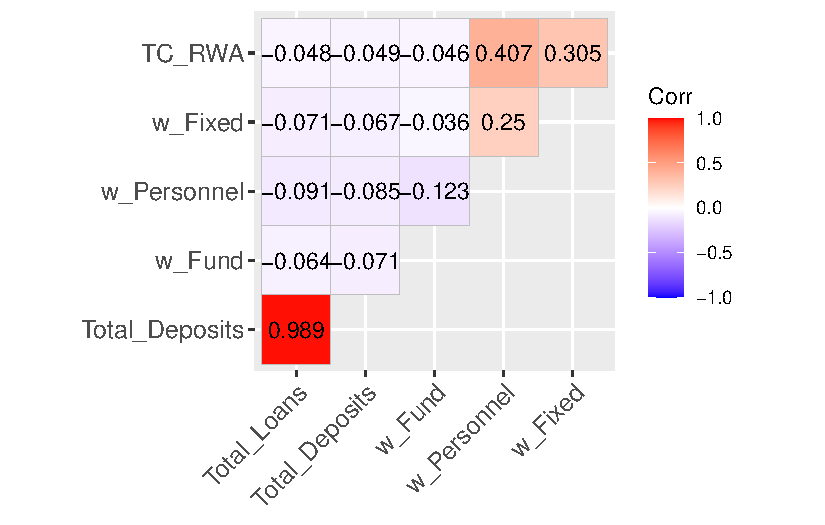
\includegraphics{chapter02-efficiency_files/figure-pdf/fig-correlationEff-1.pdf}

}

\caption{\label{fig-correlationEff}Correlation Matrix}

\end{figure}%

Figure~\ref{fig-correlationEff} reports the Pearson correlation matrix
between the predictor variables. All correlation coefficients of the
variables are lower than 0.6, except for the correlation between total
deposits and total loans due to the fact that we choose to follow the
intermediation approach and a dual approach employed by Berger and
Humphrey (1991) and Bauer et al. (1993) in our analysis.

\subsection{Main results}\label{main-results-1}

\begin{longtable}[]{@{}ccc@{}}

\caption{\label{tbl-translog}Translog cost frontier}

\tabularnewline

\toprule\noalign{}
\endhead
\bottomrule\noalign{}
\endlastfoot
~ & \multicolumn{2}{c@{}}{%
Translog Cost} \\
Variable & Estimates & std. Error \\
(Intercept) & -0.379 \textsuperscript{***} & 0.066 \\
ly1 & -0.639 \textsuperscript{**} & 0.244 \\
ly2 & 1.892 \textsuperscript{***} & 0.324 \\
lx2 & 0.027 \textsuperscript{} & 0.107 \\
lx3 & -0.454 \textsuperscript{***} & 0.081 \\
I(0.5 * ly1\^{}2) & 2.821 \textsuperscript{***} & 0.614 \\
I(ly1 * ly2) & -1.885 \textsuperscript{*} & 0.799 \\
I(0.5 * ly2\^{}2) & 1.747 \textsuperscript{} & 1.085 \\
I(0.5 * lx2\^{}2) & -0.175 \textsuperscript{} & 0.090 \\
I(lx2 * lx3) & 0.288 \textsuperscript{***} & 0.067 \\
I(0.5 * lx3\^{}2) & 0.558 \textsuperscript{***} & 0.069 \\
I(ly1 * lx2) & 0.240 \textsuperscript{} & 0.351 \\
I(ly1 * lx3) & 1.065 \textsuperscript{***} & 0.255 \\
I(ly2 * lx2) & -0.646 \textsuperscript{} & 0.435 \\
I(ly2 * lx3) & -0.904 \textsuperscript{**} & 0.320 \\
Year2011 & 0.024 \textsuperscript{***} & 0.002 \\
Year2012 & 0.035 \textsuperscript{***} & 0.002 \\
Year2013 & 0.036 \textsuperscript{***} & 0.002 \\
Year2014 & 0.045 \textsuperscript{***} & 0.002 \\
Year2015 & 0.045 \textsuperscript{***} & 0.002 \\
Year2016 & 0.031 \textsuperscript{***} & 0.002 \\
Year2017 & 0.023 \textsuperscript{***} & 0.002 \\
Year2018 & 0.030 \textsuperscript{***} & 0.002 \\
Year2019 & 0.026 \textsuperscript{***} & 0.002 \\
Year2020 & 0.012 \textsuperscript{***} & 0.002 \\
Observations & \multicolumn{2}{l@{}}{%
2121} \\
R\textsuperscript{2} / R\textsuperscript{2} adjusted &
\multicolumn{2}{l@{}}{%
0.933 / 0.932} \\
\multicolumn{3}{@{}r@{}}{%
* p\textless0.05~~~** p\textless0.01~~~*** p\textless0.001} \\

\end{longtable}

\begin{longtable}[t]{llrrr}

\caption{\label{tbl-scores}Efficiency Measures by Ownership Structure}

\tabularnewline

\toprule
Ownership & Year & Transient & Persistent & Overall\\
\midrule
\endfirsthead
\multicolumn{5}{@{}l}{\textit{(continued)}}\\
\toprule
Ownership & Year & Transient & Persistent & Overall\\
\midrule
\endhead

\endfoot
\bottomrule
\endlastfoot
\addlinespace[0.3em]
\multicolumn{5}{l}{\textbf{Foreign-owned}}\\
\hspace{1em}Foreign-owned & 2010 & 97.776\% & 95.807\% & 93.577\%\\
\hspace{1em}Foreign-owned & 2011 & 97.686\% & 95.807\% & 93.679\%\\
\hspace{1em}Foreign-owned & 2012 & 97.790\% & 95.807\% & 93.697\%\\
\hspace{1em}Foreign-owned & 2013 & 97.748\% & 95.807\% & 93.807\%\\
\hspace{1em}Foreign-owned & 2014 & 97.818\% & 95.807\% & 93.799\%\\
\hspace{1em}Foreign-owned & 2015 & 97.833\% & 95.807\% & 93.813\%\\
\hspace{1em}Foreign-owned & 2016 & 97.848\% & 95.807\% & 93.828\%\\
\hspace{1em}Foreign-owned & 2017 & 98.024\% & 95.807\% & 93.767\%\\
\hspace{1em}Foreign-owned & 2018 & 98.088\% & 95.807\% & 93.812\%\\
\hspace{1em}Foreign-owned & 2019 & 98.101\% & 95.807\% & 93.825\%\\
\hspace{1em}Foreign-owned & 2020 & 98.114\% & 95.807\% & 93.837\%\\
\addlinespace[0.3em]
\multicolumn{5}{l}{\textbf{Foreign Joint-stock}}\\
\hspace{1em}Foreign Joint-stock & 2010 & 97.992\% & 95.515\% & 93.957\%\\
\hspace{1em}Foreign Joint-stock & 2011 & 98.005\% & 95.515\% & 93.970\%\\
\hspace{1em}Foreign Joint-stock & 2012 & 98.110\% & 95.515\% & 93.941\%\\
\hspace{1em}Foreign Joint-stock & 2013 & 98.163\% & 95.515\% & 93.938\%\\
\hspace{1em}Foreign Joint-stock & 2014 & 98.278\% & 95.515\% & 93.859\%\\
\hspace{1em}Foreign Joint-stock & 2015 & 98.290\% & 95.515\% & 93.870\%\\
\hspace{1em}Foreign Joint-stock & 2016 & 98.301\% & 95.515\% & 93.882\%\\
\hspace{1em}Foreign Joint-stock & 2017 & 98.313\% & 95.515\% & 93.893\%\\
\hspace{1em}Foreign Joint-stock & 2018 & 98.325\% & 95.515\% & 93.904\%\\
\hspace{1em}Foreign Joint-stock & 2019 & 98.336\% & 95.515\% & 93.915\%\\
\hspace{1em}Foreign Joint-stock & 2020 & 98.348\% & 95.515\% & 93.926\%\\
\addlinespace[0.3em]
\multicolumn{5}{l}{\textbf{Joint-stock}}\\
\hspace{1em}Joint-stock & 2010 & 98.368\% & 94.799\% & 93.733\%\\
\hspace{1em}Joint-stock & 2011 & 98.436\% & 94.799\% & 93.678\%\\
\hspace{1em}Joint-stock & 2012 & 98.493\% & 94.799\% & 93.660\%\\
\hspace{1em}Joint-stock & 2013 & 98.644\% & 94.799\% & 93.551\%\\
\hspace{1em}Joint-stock & 2014 & 98.630\% & 94.799\% & 93.599\%\\
\hspace{1em}Joint-stock & 2015 & 98.674\% & 94.799\% & 93.568\%\\
\hspace{1em}Joint-stock & 2016 & 98.676\% & 94.799\% & 93.593\%\\
\hspace{1em}Joint-stock & 2017 & 98.707\% & 94.799\% & 93.566\%\\
\hspace{1em}Joint-stock & 2018 & 98.713\% & 94.799\% & 93.560\%\\
\hspace{1em}Joint-stock & 2019 & 98.712\% & 94.799\% & 93.570\%\\
\hspace{1em}Joint-stock & 2020 & 98.719\% & 94.799\% & 93.569\%\\
\addlinespace[0.3em]
\multicolumn{5}{l}{\textbf{Local government-holding}}\\
\hspace{1em}Local government-holding & 2010 & 98.487\% & 95.097\% & 93.730\%\\
\hspace{1em}Local government-holding & 2011 & 98.506\% & 95.097\% & 93.717\%\\
\hspace{1em}Local government-holding & 2012 & 98.518\% & 95.097\% & 93.728\%\\
\hspace{1em}Local government-holding & 2013 & 98.549\% & 95.097\% & 93.729\%\\
\hspace{1em}Local government-holding & 2014 & 98.548\% & 95.097\% & 93.752\%\\
\hspace{1em}Local government-holding & 2015 & 98.555\% & 95.097\% & 93.752\%\\
\hspace{1em}Local government-holding & 2016 & 98.580\% & 95.097\% & 93.750\%\\
\hspace{1em}Local government-holding & 2017 & 98.590\% & 95.097\% & 93.759\%\\
\hspace{1em}Local government-holding & 2018 & 98.603\% & 95.097\% & 93.762\%\\
\hspace{1em}Local government-holding & 2019 & 98.605\% & 95.097\% & 93.783\%\\
\hspace{1em}Local government-holding & 2020 & 98.578\% & 95.097\% & 93.829\%\\
\addlinespace[0.3em]
\multicolumn{5}{l}{\textbf{State-owned}}\\
\hspace{1em}State-owned & 2010 & 98.692\% & 94.841\% & 93.557\%\\
\hspace{1em}State-owned & 2011 & 98.701\% & 94.841\% & 93.566\%\\
\hspace{1em}State-owned & 2012 & 98.710\% & 94.841\% & 93.574\%\\
\hspace{1em}State-owned & 2013 & 98.718\% & 94.841\% & 93.583\%\\
\hspace{1em}State-owned & 2014 & 98.712\% & 94.841\% & 93.610\%\\
\hspace{1em}State-owned & 2015 & 98.721\% & 94.841\% & 93.618\%\\
\hspace{1em}State-owned & 2016 & 98.730\% & 94.841\% & 93.627\%\\
\hspace{1em}State-owned & 2017 & 98.738\% & 94.841\% & 93.635\%\\
\hspace{1em}State-owned & 2018 & 98.747\% & 94.841\% & 93.643\%\\
\hspace{1em}State-owned & 2019 & 98.756\% & 94.841\% & 93.652\%\\
\hspace{1em}State-owned & 2020 & 98.764\% & 94.841\% & 93.660\%\\*

\end{longtable}

The means of efficiency scores by year and by ownership structure are
presented in Table~\ref{tbl-scores}. In almost all earlier banking
efficiency studies, time-varying (transient) (in)efficiency is the only
source of inefficiency. Using the above 3-step method, we report higher
average scores than what has been found in the previous studies such as
Fungáčová et al. (2013), Pessarossi and Weill (2015) and Dong et al.
(2016).

The decomposition of the overall efficiency has been presented in
Table~\ref{tbl-scores}. We observe that transient efficiency and
persistent efficiency show every similar values and overall efficiency
ranging between 95\%-97\% across all ownership types.This result
collaborate what has been reported in Fungáčová et al. (2020).

\begin{verbatim}
TableGrob (3 x 1) "arrange": 3 grobs
  z     cells    name           grob
1 1 (1-1,1-1) arrange gtable[layout]
2 2 (2-2,1-1) arrange gtable[layout]
3 3 (3-3,1-1) arrange gtable[layout]
\end{verbatim}

\begin{figure}

\centering{

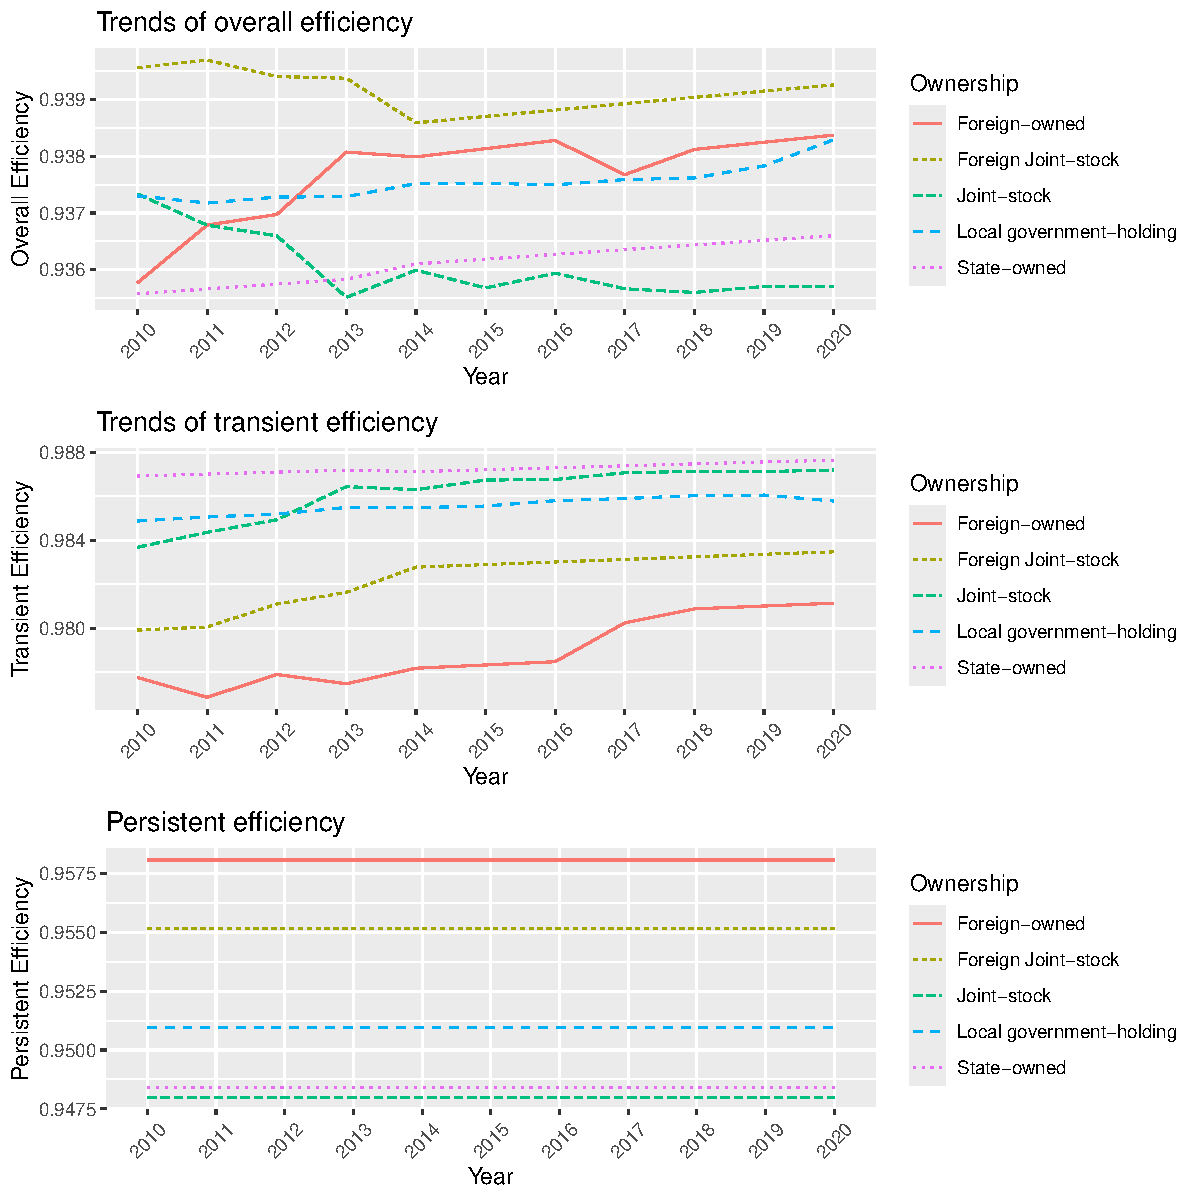
\includegraphics{chapter02-efficiency_files/figure-pdf/fig-decomposition-1.pdf}

}

\caption{\label{fig-decomposition}Changes of efficiencies by ownership}

\end{figure}%

Figure~\ref{fig-decomposition} are the visualization of
Table~\ref{tbl-scores}, from which we may draw some conclusions about
efficiency of Chinese banks. We notice that the evolution of both
overall efficiency and transient efficiency do not show high volatility
over time. This result is also in line with Fungáčová et al. (2020).

In terms of overall efficiency depending on ownership structure, we
report that state-owned banks have relatively low level of efficiency.
The trends show that the state-owned banks' overall efficiency level is
lower than foreign joint-stock banks, foreign-owned banks, and local
government-holding banks; it is also lower than (domestic) joint-stock
banks before the mid-2012. This result partially collaborates the trends
presented in the previous studies including Fungáčová et al. (2013),
Dong et al. (2016), Fungáčová et al. (2020) and Berger et al. (2009),
where they find the state-owned banks are less efficient than
joint-stock banks and foreign banks. In the above figures, the
foreign-owned banks have lower efficiency than other joint-stock types
before 2011 (except for the state-owned banks). However, the increasing
trends in overall and transient efficiency of foreign-owned banks are
clearly shown. The reasons that our results differ from the previous
study might due to the different sample periods and sample banks.
Furthermore, our study also select 12 state-owned banks based on CBIRC
definition instead of the Big five (the biggest 5 state-owned banks in
size).

By decomposing overall efficiency to transient and persistent parts,
Figure~\ref{fig-decomposition} reveals the sources which may result in
the efficiency pattern shown in fig-trends. The state-owned banks have
higher transient efficiency than other ownership types. However, the
state-owned banks have lower time-invariant efficiency than most of
other ownership banks, which can be considered as the main cause of the
medium level of overall efficiency. This finding support the results
reported by Iannotta et al. (2007) and Berger et al. (2005). The
joint-stock banks show similar pattern of relatively high transient
efficiency and the lowest persistent efficiency compared to other
ownership types.

According to Colombi et al. (2011), Filippini and Greene (2016),
Kumbhakar et al. (2015), transient (in)efficiency component has the
feature of time-varying which captures the short-term pattern of
(in)efficiency. Transient inefficiencies might be attributed to
short-term management moral hazard and/or adverse selecting problem.
Firms can take some time to solve short-term deviation from expected
operating behavior. Time-invariant inefficiency, on the other hand,
captures persistent inefficiency which stems from structural rigidities
of the organization and the production process, as well as regulatory
constrains on the firm. It is reasonable to assume that these sources of
inefficiency remain constant and stay with the firm over time. The
joint-stock banks have relatively high transient efficiency level which
may reveal those banks are more flexible and efficient in dealing with
short-term sub-optimal resource allocation and adjusting costs. However,
the low persistent efficiency could indicate these banks may have
long-run moral hazard problems and/or respond negative to regulatory
constrains.

The similar pattern has been revealed in the state-owned banks. However,
due to the sizes and ownership structure of the state-owned banks are
quite different from the joint-stock banks, the interpretation could be
different. Over 50\% of shareholding in city banks and over 87\% of
shareholding in rural commercial banks (most of these banks have the
join-stock ownership structure) are private enterprises which can be
considered as small and medium businesses (SMEs) by 2017. The
state-owned banks are much larger than the joint-stock banks in assets.
The high transient efficiency may demonstrate that the state-owned banks
have benefit of economies of scale. Badunenko and Kumbhakar (2017) state
that the state-owned banks have a larger portion operating under scale
economies than other ownership types in the post re-regulation period,
using the empirical data in Indian banking. The results reveal that the
state-owned banks have lower persistent efficiency than almost all other
ownership types. Instead of structural problems, we suggest that the low
persistent efficiency might be attributed to the characteristics of
business of the state-owned banks in China's banking industry. This
finding, to some extent, supports the viewpoint that state-owned banks
would be involved in policy-guided credit activities instead of
profit-centered ones (Pessarossi and Weill, 2015). The social lending
theory of state ownership (see Atkinson and Stiglitz, 1980) suggests
that state-owned enterprises contribute to ``correcting the `failure' of
market economy'' due to imperfect competition, inefficiency and public
good. According to this view, government-owned enterprises may help
improve the overall economy performance (Stiglitz, 1993). In China's
banking context, the biggest four commercial banks were founded and
conducted a large amount of government lending in the early 1990's,
before national banks and city banks were established. Within a
relatively long period, the state-owned banks (including local
government-holding banks founded later in the end of 1990's) played a
role of `government agencies' to pursue the broader social welfare
objectives rather than profit maximizing, for example, the projects of
the nationwide High-speed Rail network. Since 2001, the ownership
structure has been dramatically transformed, due to China's overall
industrial reforms and the commitments to the WTO agreement. The state
shareholder was replaced by Central Huijin Investment Ltd.~The
state-owned banks are still the main funding providers for nationwide
infrastructure projects focusing on social welfare due to the huge
amount of financing required and the complexity of structure of
financing. Since the state-owned banks target multiple welfare
objectives which might not be measurable, it is reasonable to draw a
conclusion that the state-owned banks suffer low persistent efficiency
over time.

\subsection{Inefficiency effects}\label{inefficiency-effects}

\begin{longtable}[]{@{}ccc@{}}

\caption{\label{tbl-effects}Inefficiency effects}

\tabularnewline

\caption{Inefficiency Effects}\tabularnewline
\toprule\noalign{}
\endfirsthead
\endhead
\bottomrule\noalign{}
\endlastfoot
~ & Transient Efficiency & Persistent Efficiency \\
Variable & Estimates & Estimates \\
(Intercept) & 0.983 \textsuperscript{***} & 0.956
\textsuperscript{***} \\
OwnershipForeign Joint-stock & 0.000 \textsuperscript{} & -0.000
\textsuperscript{} \\
OwnershipJoint-stock & 0.004 \textsuperscript{***} & -0.008
\textsuperscript{***} \\
OwnershipLocal government-holding & 0.004 \textsuperscript{***} & -0.005
\textsuperscript{***} \\
OwnershipState-owned & 0.005 \textsuperscript{***} & -0.008
\textsuperscript{***} \\
TC\_RWA & -0.021 \textsuperscript{***} & 0.004 \textsuperscript{} \\
Observations & 1993 & 2186 \\
R\textsuperscript{2} / R\textsuperscript{2} adjusted & 0.061 / 0.058 &
0.040 / 0.038 \\
\multicolumn{3}{@{}r@{}}{%
* p\textless0.05~~~** p\textless0.01~~~*** p\textless0.001} \\

\end{longtable}

Following Colombi et al. (2017) and Fungáčová et al. (2020), we
parametize the inefficiency terms through linear models in
``Methodology'' section. The estimates are presented in
Table~\ref{tbl-effects}. The estimates suggest a statistically
significant negative relationship between regulatory capital
requirements and transient (time-varying) efficiency, but no significant
relationship between capital adequacy and persistent (time-invariant)
efficiency. This finding partially supports the results in Barth et al.
(2004) where they find capital stringency is not strongly linked with
bank efficiency where they use different measure of bank efficiency.
Similarly, Lee and Chih (2013), Djalilov and Piesse (2019), and
Lešanovská and Weill (2016) also do not find sufficient evidence to
support a statistically significant relationship between capital
regulation and bank efficiency. However, Barth et al. (2013) find that
greater capital regulation stringency is negatively associated with bank
efficiency. Our finding shows that that Basel III capital regulation can
influence commercial banks' decisions and perspectives on cost
constainment strategies which are closely associated time. This can be
provided as part of research evidence of the development of the Basel
framework.

From the agency theory perspective, this finding may support the
viewpoint provided in Lešanovská and Weill (2016): the two agency costs
caused by ``asset substitution'' (see Smith and Warner, 1979) and
``control hypothesis'' (see Jensen, 1986), respectively, may have the
effect of offsetting each other. The reforms in China's banking industry
took further steps following the WTO agreement in 2001. The joint-stock
banks (including local government-holding banks, city banks, and rural
commercial banks) have become the mainstream of Chinese banks. The
modern corporate governance framework has been established in banks.
Transformation in ownership structure has accelerated development of
banks regarding assets growing and branch expansion; and has also raised
the conflict between shareholders and managers over the free cash flow
(``control hypothesis''). On the other hand, the rapid development of
capital markets provides more funding channels for banks such as public
offering and inter-bank funding. The changes make banks less dependent
on debt financing, which may lessen the conflict between shareholders
and creditors. Therefore, the impact of capital reserve on efficiency
could reflect the result of the offset of these two agency costs.

In terms of the impact of ownership structure on bank cost efficiency,
the state-owned ownership type shows a statistically significant result,
however, inconclusive. Combining with the results presented in
tbl-scores, we believe that it could be reasonable to assume lower cost
efficiency of state-owned banks. Since 2001, direct state-stakes in
state-owned banks has been replaced by a Central Huijin
shareholder-stake, along with the establishment of modern corporate
governance system. We argue that the direct state intervention has
transformed, instead of state ownership, but into state concentrated
ownership which is an ownership type similar to the one of large
investors with significant control rights and cash flow rights (``large
investors,'' see Shleifer and Vishny, 1997). From this perspective,
concentrated ownership puts pressure on management decision making
(Shleifer and Vishny, 1997) and therefore bank performance. Justified by
the theory of property rights (see Berle and Means, 1932) and the theory
of agency (see Jensen and Meckling, 1976), state concentrated ownership
could create decisive power and may favor particular projects. Sapienza
(2004) finds that state-owned banks favor large firms and charge lower
interest rates than other types of banks in Italy. Rather than political
patronage (see Sapienza, 2004), China's state-owned banks support
projects with potential of social-benefits rather than those with target
of profit-maximizing. Therefore, state-owned banks suffer lower cost
efficiency thank other ownership types.

\section{Conclusion}\label{conclusion-2}

This study aims to analyze cost efficiency of commercial banks in
China's banking industry and explore the impact of regulatory capital
and ownership structure on banks' cost efficiency in Basel III era
following 2007-2009 global financial crisis. This period we choose
(2010-2020) coincides with the fourth stage of China's financial reform
and the implementation of Basel III framework in China. We analyze cost
efficiency using in total 2574 annual observations over the period
2010-2020 on 233 commercial banks in China with 5 types of ownership
structure - state-owned, local government holding, joint-stock, foreign
joint-stock, and foreign owned. Our data covers over 91\% of total
assets in China's banking industry. We employ a four-component panel
stochastic cost frontier model developed by Colombi et al. (2011),
Colombi et al. (2014), Filippini and Greene (2016) and Kumbhakar et al.
(2015) in the most recent years, decomposing the cost inefficiency into
transient and persistent components, to investigate bank cost efficiency
and inefficiency effects. In addition, we provide background information
on China's financial reform regarding evolution of ownership structure.

Our empirical results show that transient efficiency and persistent
efficiency have very similar values which suggest that overall
inefficiency decomposes almost equally between these two components. The
state-owned banks have the overall efficiency ranking in the middle
across the ownership types, with higher transient efficiency and much
lower persistent efficiency. This finding collaborates the findings by
Fungáčová et al. (2020).

Our investigation to the impact of regulatory capital requirements on
bank cost efficiency reveals that Basel III capital regulation is
negatively associated with transient(time-varying) (in)efficiency but
shows no statistically relation to persistent(time-invariant)
(in)efficiency. Our findings partially support the results by Barth et
al. (2004), Lee and Chih (2013), Djalilov and Piesse (2019) and
Lešanovská and Weill (2016), but differ from other previous studies. We
provide the explanation for the different efficiency level between
different ownership structure and the reason why the state-owned banks
suffers low efficiency over time based on historical and theory
perspectives. Based on the findings outlined above, the study proposes
several policy recommendations. Firstly, because Basel III capital
adequacy requirements have a negative impact on banks' transient
(in)efficiency, China's regulatory authorities may set up a
well-established, dynamic framework to address banks' cost containment
strategies as well as control the risk-taking behaviors. Secondly,
Chinese regulators may leverage the insights and methodology of this
study. With more complete data sets, regulators can establish further
detailed analysis on the determinants of banks' (in)efiiciency.
Internationally, regulators may also conduct similar analyses using
local bank-level data to ascertain the Basel III framework's
approporiateness within their respective jurisdictions. Lastly, the
study reinforce the necessity of consolidation of the Basel III
regulatory framework by revealing the diversed relation between capital
regulation and bank transient /persistent efficiency. Regulators may
compelate employing the mix of Basel III variables not only to sheild
banks from potential economic and financial turbulence but also uphold
banks' efficiency.

\subsection{Bias and Further
Directions}\label{bias-and-further-directions}

This study employs a four-component SF model that has been introduced
and developed by Colombi et al. (2011), Colombi et al. (2014), Filippini
and Greene (2016), and Kumbhakar et al. (2015), and separates the random
firm effects from banks' persistent(time-invariant) inefficiency and
transient(time-varying) inefficiency. The model has the assumption that
all the error components are independently and identically distributed
(i.i.d.) random variables. Estimation of the model can be conducted in a
single stag Maximum Likelihood method based on distributional
assumptions on the four components (Colombi et al., 2011). In
consideration of our data availability, we conduct a three-step method
to estimate the model. According to Battese and Coelli (1995), a
multi-step method where the final stage involves the specification of a
regression model for the predicted inefficiency effects may contradict
the distributional assumption of i.i.d., thereby causing the biased
estimation.

Regarding further direction of our research, we intend to explore the
heteroskedastic four-component model (see Badunenko and Kumbhakar, 2017)
in which error component variances are functions of covariates that are
determinants of inefficiency and try the single step Maximum Likelihood
mothod in estimation. We will also consider conducting comparative
analyses with banking sectors in other emerging markets undergoing
similar regulatory changes, such as Brazil. The comparative analyses can
offer valuable insights. Countries experiencing analogous shifts in
regulatory frameworks may provide useful comparative data to assess the
generalizability and robustness of our findings. Exploring how different
regulatory environments impact banking practices and performance metrics
across diverse emerging economies could enrich our understanding of the
broader implications of regulatory reforms.

\newpage

\section{Appendix}\label{appendix}

\subsection{The Variable Definition Table for Efficiency
Analysis}\label{the-variable-definition-table-for-efficiency-analysis}

\begin{table}

\caption{\label{tbl-variablesEff}Variable Definition}

\centering{

\centering\begingroup\fontsize{10}{12}\selectfont

\resizebox{\ifdim\width>\linewidth\linewidth\else\width\fi}{!}{
\begin{tabular}[t]{ll>{\raggedright\arraybackslash}p{6cm}>{\raggedright\arraybackslash}p{4cm}}
\toprule
\textbf{Variable} & \textbf{Acronym} & \textbf{Definition} & \textbf{Data Source}\\
\midrule
\addlinespace[0.3em]
\multicolumn{4}{p{\linewidth}}{\textbf{Cost Frontier Variables\_Output}}\\
\hspace{1em}\cellcolor{gray!10}{Cost Frontier Variables\_Output} & \cellcolor{gray!10}{Total Gross Loans} & \cellcolor{gray!10}{Loans and finance leases held for investment or held for sale, net of unearned discount and gross of loss reserves. Does not include accrued interest on loans.} & \cellcolor{gray!10}{SNL Database and bank annual reports}\\
\hspace{1em} & Total Deposits & Total deposits from customers. For US banks, this is the total deposits from customers and banks. & SNL Database and bank annual reports\\
\addlinespace[0.3em]
\multicolumn{4}{p{\linewidth}}{\textbf{Cost Frontier Variables\_Input Price}}\\
\hspace{1em}\cellcolor{gray!10}{Cost Frontier Variables\_Input Price} & \cellcolor{gray!10}{Price of funds} & \cellcolor{gray!10}{Interest Expense/Total Deposits} & \cellcolor{gray!10}{Manually compuation based on SNL Database and bank annual reports}\\
\hspace{1em} &  & Interest Expense: Interest on debt and other borrowings, on an incurred basis. Includes the amortization of discount or premiums and interest on capital leases. & SNL Database and bank annual reports\\
\hspace{1em}\cellcolor{gray!10}{} & \cellcolor{gray!10}{Price of labor} & \cellcolor{gray!10}{Personnel Expense/Total Assets} & \cellcolor{gray!10}{Manually compuation based on SNL Database and bank annual reports}\\
\hspace{1em} &  & Total Assets: All assets owned by the bank as of the date indicated, as carried on the balance sheet and defined under the indicated accounting principles & SNL Database and bank annual reports\\
\hspace{1em}\cellcolor{gray!10}{} & \cellcolor{gray!10}{} & \cellcolor{gray!10}{Personnel Expense: Salaries, wages, bonuses, commissions, changes in reserve for future stock option expense, and other employee benefit costs. Includes any expenses related to employment or retirement benefits, whether paid or deferred, recognized during the period.} & \cellcolor{gray!10}{SNL Database and bank annual reports}\\
\hspace{1em} & Price of fixed assets & Other Operating Expense/Fixed Assets & Manually compuation based on SNL Database and bank annual reports\\
\hspace{1em}\cellcolor{gray!10}{} & \cellcolor{gray!10}{} & \cellcolor{gray!10}{Other Operating Expense: Operating Expense excludes Personnel Expense} & \cellcolor{gray!10}{Manually compuation based on SNL Database and bank annual reports}\\
\hspace{1em} &  & Fixed Assets: Property, plant and equipment acquired for long-term use in normal operations. Fixed assets are carried at cost, net of accumulated depreciation. & SNL Database and bank annual reports\\
\addlinespace[0.3em]
\multicolumn{4}{p{\linewidth}}{\textbf{Total Costs}}\\
\hspace{1em}\cellcolor{gray!10}{Total Costs} & \cellcolor{gray!10}{TC} & \cellcolor{gray!10}{The sum of interest expense, personnel expense and othe operating expenses} & \cellcolor{gray!10}{Manually compuation based on SNL Database and bank annual reports}\\
\addlinespace[0.3em]
\multicolumn{4}{p{\linewidth}}{\textbf{Determinants of Inefficiency}}\\
\hspace{1em}Determinants of Inefficiency &  &  & \\
\hspace{1em}\cellcolor{gray!10}{Regulation} & \cellcolor{gray!10}{TC\_RWA} & \cellcolor{gray!10}{Total Regulatory Capital/Risk Weighted Assets, Total capital ratio as defined by the latest regulatory and supervisory guidelines.} & \cellcolor{gray!10}{SNL Database and bank annual reports}\\
\hspace{1em}Ownership &  & Ownership categories and definitions listed in Table 1 & \\
\hspace{1em}\cellcolor{gray!10}{Bank Size} & \cellcolor{gray!10}{LnAssets} & \cellcolor{gray!10}{Natrual Logarithm of Total Assets, as an indicator of the size of a bank} & \cellcolor{gray!10}{Manually compuation based on data of Total Assets}\\
\bottomrule
\end{tabular}}
\endgroup{}

}

\end{table}%

\bookmarksetup{startatroot}

\chapter{Assessing Systemic Risk Dynamics in Chinese Banking: The Impact
of Basel III and Ownership
Structures}\label{assessing-systemic-risk-dynamics-in-chinese-banking-the-impact-of-basel-iii-and-ownership-structures}

\section{Introduction}\label{introduction-3}

The 2007-2009 Global Financial Crisis (GFC) triggered an overhaul of
financial regulation system. Seeking to address structural weaknesses of
pre-crisis banking regulation, the Basel III framework (Basel III),
based on the regulatory reform agenda endorsed by Group of Twenty (G20)
leaders in 2009, was finalized in 2017. Regulatory consensus has focused
on increasing capital adequacy requirements and liquidity assessment, in
recognition of that banks should be subject to more stringent capital
regulation (Demirgüç-Kunt et al., 2018). The updated Basel regulatory
framework (Basel III) focuses on systemic risk and macro-prudential
regulation designed to enhance the banking sector's resilience and
strengthen risk management practices, and mitigate the potential for
systemic risk. As one of the member countries of Basel Committee on
Banking Regulation and Supervision (BCBS), China has been at the
forefront of implementing Basel III framework.

China's banking sector, marked by its rapid growth and increasing
integration into the global financial system, plays a crucial role in
sustaining the country's economic development. China's banking sector
underwent fundamental changes in 1978, as part of China's overall
economic reform. Since 2001, when China got accession to the World Trade
Organization (WTO), the reform of China's banking industry has stepped
up its pace and the entire banking sector has been dramatically
reshaped. The reform has transformed Chinese banks into market-oriented
enterprises, changed their ownership structure, established modern
corporate governance mechanisms, and introduced legislation and
regulatory framework. Since 2010, improvements and refinements have
continued in China's banking sector and entered the advanced stage of
the reform. In the wake of the GFC, Chinese regulatory authorities have
proactively embraced the Basel III framework, aiming to fortify the
national financial system against potential shocks. The evolution of
China's banking landscape presents a unique context for investigating
the implementation of Basel III regulation. A rich body of literature
focusing on the previous stages of the reform assesses the relationship
between capital requirements and Chinese banks' performance and
standalone risk including Pessarossi and Weill (2015), Tan and Floros
(2013), and Lee and Chih (2013). By exploring the relationship between
risk-based regulatory capital requirements and systemic risk in China's
banking sector, this study aims to provide insights for regulators,
policymakers and market participants in the context of China's financial
environment.

Building upon our previous investigations in Chapter 3, which focused on
the influence of Basel III on banks' credit risk-taking, and Chapter 4,
which dissected efficiency dynamics within China's banking sector, this
chapter further enriches our understanding of financial stability. In
this paper, we extend existing empirical research studying the dynamic
between Basel III capital adequacy requirements, systemic risk and
ownership structure in China's banking sector. Notwithstanding the
policy consensus, economic theories are split on the impact of capital
on standalone risk. Some theories emphasize that bank capital acts as a
buffer to absorb shocks (e.g. Repullo, 2004) and higher capitalization
optimize the borrower screening (e.g. Allen et al., 2011). Other
theoretical literature claims that capital regulation may exacerbate
banks' portfolio risk and reduce bank stability (see Koehn and
Santomero, 1980). Since the early 2000s, academic literature started to
direct its focus towards systemic risk. Systemic risk is defined by De
Bandt and Hartmann (2019) as ``the risk of experiencing systemic events
in the strong sense''. Pioneering works by Allen and Gale (2000) study
the diffusion of financial contagion via multiple channels in reaction
to an initial small chock. After the GFC, the approach to identify the
mechanisms of driving systemic risk has been directed to tail
interdependences between market indices (Acharya et al., 2017; see
Adrian and Brunnermeier, 2016). Laeven et al. (2016) and Demirgüç-Kunt
et al. (2018) examine the relation between Basel III capital regulation
and systemic risk using cross-country data employing the approaches
proposed by these two studies. Both of the studies find that there is a
negative relationship between capital regulation and systemic risk. The
investigation of the relationship between capital and systemic risk in
Chinese banking sector is relatively scarce in the current body of
research. Recent studies have focused on systemic risk in Chinese
financial system. Wang et al. (2018) investigate the systemic risk of
China's financial institutions employing tail-event networks. Huang et
al. (2019) examine systemic risk in Chinese banking system by employing
multiple measures to capture different aspects of systemic risk of
Chinese banks.

This paper provides empirical evidence using forensically analysed data
on 376 Chinese financial institutions over the period 2010-2022. Because
our focus is on the dynamics of systemic risk and Chinese banks, we hand
collect the ownership structure information of these 236 Chinese
commercial banks and classify them into five categories of ownership
identities: State-owned (Big Six and other than Big Six), Local
government-holding, Joint-stock, Foreign joint-stock, and Foreign-owned
banks (Table~\ref{tbl-banks}). We compute conditional value at risk
(CoVaR) proposed by Adrian and Brunnermeier (2016). We expect risk-based
capital regulation to have a negative impact on the individual banks'
contribution to systemic risk.

Consistent with the theoretical literature that emphasizes bank capital
as a buffer in absorbing economic shocks, we find that higher regulatory
capital reduces individual banks' contribution to systemic risk. Our
results show that systemic risk increased with bank size. We also find
evidence that state-ownership make higher contribution to systemic risk
compared to joint-stock and local government-holding structure.

This paper contributes to the literature in several ways. First, our
research bridges the global regulatory framework and the localized
implementation in the Chinese context. This study provides insights into
how global financial regulatory standards interact with the specificity
of Chinese national banking system. China has become a major player in
the global financial system by internationally integrated and closely
interconnected with financial institutions. China fully adopted Basel
III framework as part of its ``open-door'' economic reform.
Understanding how Basel III framework interact with the idiosyncrasies
of China's banking industry contributes not only to academic research,
but also informs policymakers and stakeholders about potential areas of
concern or improvement, regarding the challenges of fostering global
financial stability.

Second, our study contributes to the extant literature on systemic risk
by analyzing the effect of ownership structure on systemic risk. The
study examines the influence of different ownership structures on
systemic risk in the Chinese banking sector. Our findings that state
ownership influences systemic risk through factors including
shareholding concentration, significant cash flow rights, and asset size
provide new insights into the determinants of systemic risk; and
facilitate the ongoing efforts to design effective and targeted
regulatory measures that improve overall financial stability.

Third, this study fills a gap in the existing literature by focusing on
the Chinese banking sector's systemic risk in relation to capital
regulation. Most existing literature focus on European and the US banks.
Research focusing on the Chinese banks' contribution to systemic risk is
still scares. This is a relatively under-explored area in current
research, especially post-implementation of the Basel III framework in
China.

Finally, The paper provides empirical evidence using data on 376 Chinese
financial institutions over the period 2010-2022. This extensive data
allows for a comprehensive analysis of the dynamics between systemic
risk and regulatory capital in a unique national implementation context.

The remainder of this paper is organised as follows. Section II reviews
related literature, as well as a brief introduction of the evolution of
ownership structure of commercial banks in China. Section III presents
the data set and the empirical model including the variables considered
in our analysis. The empirical results are presented in section IV. And
section V concludes.

\section{Literature Review}\label{literature-review-1}

\subsection{Capital Regulation and Bank
Risk}\label{capital-regulation-and-bank-risk}

Bank capital affects individual banks' risk as well as a bank's
contribution to systemic stability (Demirgüç-Kunt et al., 2018). Policy
makers have consensus on increasing the stringency of capital adequacy
requirements. However, economic theories offer split views on the impact
of capital on bank risk; and empirical studies provides mixed findings.

The Basel framework, centered with the strict capital regulation, is
designed to reduce bank risk and enhance bank resilience. Theoretical
papers such as Repullo (2004) and Von Thadden (2004) support this view
that risk-based bank capital is a more efficient regulatory tool and
acts as a buffer in absorbing economic shocks and strengthens systemic
stability. Demirguc-Kunt et al. (2013) find that a strong capital
position helps banks resist earning shocks and have higher probability
to survive the crisis. They also find evidence to advocate higher
quality capital, i.e., Tier 1 capital, in the regulatory capital
requirements. These views are consistent with one of the most important
purpose of the strict capital regulation: improving banks' survival
probability. Another reason why stringent capital requirements are
considered to be effective is that they refine banks' risk management
and curb excessive risk-taking incentives. A number of theories
highlight that risk-based capital, more effective than interest rate
ceilings, boosts banks' ``franchise value,'' improves borrowers
screening, and lowers banks' excessive risk-taking incentives (Allen et
al., 2011; Mehran et al., 2011; Repullo, 2004). Other theories emphasize
a moral hazard perspective, arguing that effective regulatory
capitalization may offset the excessive risk-taking incentives created
by deposit insurance (Demirguc-Kunt and Kane, 2002,; Keeley, 1990). In
terms of Chinese commercial banks, Tan and Floros (2013) find a
significant negative relationship between bank capital and risk. Lee et
al. (2015) report that bank capital is negatively related to NPL and
support theories with the moral hazard view.

On the other hand, some research posit that greater capital regulations
may induce higher bank risk. Cooper and Ross (2002) extend the research
of Diamond and Dybvig (1983), stating that the existence of deposit
insurance weakens the depositors' incentive to monitor banks and causes
them to engage in excessive risk-taking activities. Blum (1999) suggests
that banks may have higher incentives to raise risk due to the binding
capital adequacy requirements. Calem and Rob (1999) find a U-shaped
relationship between bank capital position and risk. The risk-taking
first decreases with the increase of bank capital; then it increases as
bank capital increases on its high level. They also argue that the
increase in capital adequacy requirements induces banks to take
additional portfolio risk even if they are well-capitalized. Using
Chinese banking data, Lee and Chih (2013) find that the negative
relationship between capital and risk only exists in the sub-sample of
small banks and is not found in the sub-sample of large banks.

With regards to systemic risk, individual-bank models are only part of
the story. The banking literature has developed theoretical models to
explain systemic risk in recent years. Systemic risk may be associated
with models of contagion and macroeconomic shocks and endogenous
procyclicality (Acharya et al., 2017; Adrian and Brunnermeier, 2016; De
Bandt and Hartmann, 2019). Chen (1999) extends Diamond and Dybvig (1983)
bank run model with the rational herding approach and claims that
failures of few banks can trigger runs on other banks, caused by the
first-come, first-serve rule and information externalities. Rochet and
Tirole (1996) present a model of the interbank market and argue that
failures of large insolvent bank could induce contagion risk and
propagate through the whole financial system. Kaufman and Scott (2003)
provide one of the definitions of systemic risk focusing on spillovers
of an initial external shock which causes fire-sale driven changes both
in liquidity and interest rates. Allen and Gale (2000) set up a model
and explain financial contagion by the structure of the banking network.

Higher capital may absorb unexpected losses from macro-shocks (Kaufman
and Scott, 2003). Capital requirements imposed on the interbank lending
may reduce contagious defaults (Demirgüç-Kunt et al., 2018; Rochet and
Tirole, 1996). The joint failure risk of individual banks, arising from
the highly correlated asset returns, could cause systemic or aggregate
risk (Acharya, 2009). Correlated bank failures also produce prohibitive
social costs and capital regulation has different effect on bank risk
when multiple Nash equilibria are created by the presence of the
bail-out or central bank as lender of last resort (LOLR) (Acharya et
al., 2016). On one hand, high leverage can reduce the moral hazard
caused by managers seeking rent and providing inadequate loan monitoring
(Calomiris and Kahn, 1991). On the other hand, sufficient bank capital
ameliorates the asset-substitution moral hazard created by banks taking
excessively risk (Bhattacharya et al., 1998); hence decreases systemic
risk arising from high correlation of asset returns (Acharya, 2009).

The evidence on the linkage between capital regulation and systemic risk
in Chinese banking industry is limited in literature. Not until recent
years (after Chinese banking regulatory authority fully adopted the
Basel III framework in 2013) that researches of systemic risk in Chinese
banking sector emerged. Gang and Qian (2015) study the effect of China's
monetary policies on systemic risk and find the systemic risk has been
increased by monetary policy shocks. Huang et al. (2019) examine
systemic risk in Chinese banking system by employing multiple measures
to capture different aspects of systemic risk of Chinese banks. Zhang et
al. (2021) focus on the impact of liquidity creation on systemic risk in
Chinese banking industry and report a ``U shape'' relationship between
liquidity creation and systemic risk. They report that systemic risk is
positively related to bank liquidity creation when a bank is broadly
connected with the entire financial system. Bellavite Pellegrini et al.
(2022) evaluate the contribution of different financial sectors to
systemic risk including traditional banks, shadow banks and real estate
financial services. Liu et al. (2021) employ the MIxed DAta
Sampling(MIDAS)-Quantile Regression(QR)-CoVaR approach to measure
Chinese banks' systemic risk during the financial turmoils in 2010-2020.
They find that bank leverage and market risk coefficient(Beta) are
positively related to the systemic risk.

Building on the existing theoretical framework, our paper is related to
a number of empirical studies focusing on identifying the drivers of
systemic risk after the GFC. Anginer and Demirguc-Kunt (2014)
investigate the impact of bank capital on systemic risk by employing
various definitions of capital. They find that greater capital reduces
fragility of finanfical system as a whole. Laeven et al. (2016) study
the individual bank factors that determine systemic risk. They find that
systemic risk is positively related to bank size and inversely related
to bank capital.

\subsection{Ownership Structure and Bank
Risk}\label{ownership-structure-and-bank-risk}

The theory of ownership stems from the pioneering work of the property
rights theory by Coase (1937), Alchian (1965), Demsetz (1966), and
Alchian and Demsetz (1972); was extended by Grossman and Hart (1986) and
Hart and Moore (1990), and integrated with the agency theory by Jensen
and Meckling (1976), Fama (1980), and Fama and Jensen (1983). The
property rights theory defines ownership as residual right to income
(Alchian and Demsetz, 1972) and residual right to control (Burkart et
al., 2003); and states that the owners' property rights have been
attenuated by managers' diverting the firm's resources to their own ends
(Furubotn and Pejovich, 1972). The property rights theory allows the
prediction of behavioral consequences of individuals in the contractual
relations (De Alessi, 1980). According to the theory literature, the
impact of bank ownership structure should be considered in the context
of principal-agent framework and public choice theory (Altunbas et al.,
2001; Sapienza, 2004), focusing on shareholder rights (the degree of
ownership concentration) and the nature of the shareholders (see
Shleifer and Vishny, 1997).

The separation of ownership and control in modern corporations is an
essential part of the theory of the firm (see Berle and Means, 1932).
From the perspective of agency theory, shareholder rights and ownership
concentration are two common approaches to influence managerial behavior
and thereby impact corporate performance. It is often believed that the
diffused ownership would increase the power of managers and reduce their
dependence on the owners (Berle and Means, 1932). Alchian and Demsetz
(1972) argue that, in a corporation with dispersion of shareholding,
control may be facilitated by turning shareholders' votes into voting
blocs, which strengthens shareholders' power. Amihud and Lev (1981) and
Hirshleifer and Thakor (1992) argue that strong shareholder rights
(better investor protection) constrain managers' conservative
(sub-optimal) risk-taking choices. John et al. (2008) conduct a
cross-country study and support this view. They find the positive
relationship between investor protection and corporate risk-taking.
However, Burkart et al. (2003) present a model arguing that great
protection of shareholder rights constrains managerial discretion, which
reduces the need for dominant shareholders in order to prevent managers'
shirking behavior (Shleifer and Vishny, 1986).

Alchian and Demsetz (1972) state that firm control can be facilitated by
unrestricted salability of stock. Share trading may temporarily reform
the ownership structure, converting the diffused ownership into decisive
power blocs. Decisive power is one of the characteristics of large
shareholders. Ownership concentration, or large shareholders, is defined
as shareholders having concentrated control rights with significant cash
flow rights (Shleifer and Vishny, 1997). The model presented by Shleifer
and Vishny (1986) to estimate the value of ownership concentration. They
propose that a presence of a large shareholder may lead to
value-increasing takeovers. However, Grossman and Hart (1988) argue that
large shareholders might try to maximize their private benefit at the
expense of other small shareholders if their high control rights are not
associated with high cash flow rights. The model employed by Grossman
and Hart (1988) shows that this happens if there is a substantial
departure from one share-one vote structure. Saunders et al. (1990)
argue that stockholder controlled banks have stronger motivation to take
higher risks than banks controlled by managers/insiders. Smith and
Warner (1979) and Laeven and Levine (2009) provide empirical evidence
supporting banks with concentrated shareholding generally have higher
risk.

\subsection{State Ownership}\label{state-ownership-2}

State ownership is regarded as one of the special corporate
arrangements. In agency theory, state firms are defined as being
\emph{``controlled by the public; and the de facto control rights
usually belong to bureaucrat shareholders with highly concentrated
control rights and no significant cash flow rights''} (Shleifer and
Vishny, 1997). According to this view, state shareholders
(directly-holding shares) can be considered as a special form of large
investors with highly concentrated control rights and lack of cash flow
rights.

There are two alternative theories in the literature regarding state
ownership in banks: the social view and the political view. The social
view, based on the economic theory of institutions, suggests that state
ownership is a form of government intervention which addresses market
failures and improves market functions and economic performance
(Stiglitz, 1993). According to this view, state-owned banks may finance
those projects which might not be profitable but might have a high value
of social welfare. Therefore, state-owned banks may have poorer
performance in terms of profitability along with higher default risk
compared to their counterparties in the private sector. In contrast, the
political view claims that state ownership creates sources of political
benefits for politicians rather than social welfare. For example,
excessive employment of state firms only benefits those who support
government politically (Shleifer and Vishny, 1994). Shleifer and Vishny
(1997) suggest that state-owned firms are inefficient because the state
shareholders, with highly concentrated control rights and no cash flow
rights, only maximize their political goals which may jeopardize social
welfare.

A body of literature investigate the impact of state ownership of banks,
from both the macroeconomic angle and the perspective of individual
banks, mostly on economic growth and bank performance. Andrianova et al.
(2012) find that state ownership of banks improves countries' long-run
economic growth and make positive contributions to economic growth. On
the contrary, La Porta et al. (2002) find that higher government
ownership is related to lower economic growth. Beck and Levine (2002)
find no supporting evidence for either the social view or the political
view, regarding the role that state-owned banks played in the economy.
Beck et al. (2004) argue that state ownership intensifies bank
concentration and exacerbates financing obstacles. Sapienza (2004)
claims that state-owned banks favor large firms in banking lending,
which can be explained by political view. Berger et al. (2005) and
Berger et al. (2009) find that state-owned banks have lower
profitability and poor long-term performance.

Ownership structure of banks in China's financial markets has attracted
academic attention since China obtained accession to the WTO in 2001.
Many studies focusing on bank efficiency report that state-owned banks
exhibit lower efficiency compared to joint-stock banks and foreign banks
(Berger et al., 2009; Fungáčová et al., 2013). Several research papers
focus on ownership structure and standalone bank risk. Tan and Floros
(2013) argue that state-owned banks have higher volume of non-performing
loans and lower profitability. Zhu and Yang (2016) report that
state-owned banks take higher risk than foreign banks in China. Bai et
al. (2020) state that the issues of non-performing loans and moral
hazard are increased in state-owned banks due to the implicit government
support. However, the evidence on the linkage between ownership
structure and systemic risk is still scarce. Morelli and Vioto (2020)
report that the Chinese banking sector contributes the most to systemic
risk among the sectors of insurance, brokerage, and real estate. They
also suggest that the reduced level of bank competition due to a strong
government role in the banking sector (Jiang et al., 2019) leads to the
increase of systemic risk. Bellavite Pellegrini et al. (2022) find that
systemic risk is positively associated with the size of financial
institutions, which supports the empirical results of Laeven et al.
(2016).

Our paper extends the empirical literature studying the determinants of
systemic risk. Apart from systemic risk is influenced by bank capital,
existing literature has found that systemic risk is associated with bank
size (Laeven et al., 2016), institutional environment (Demirgüç-Kunt et
al., 2018), bank liquidity creation (Zhang et al., 2021), and the
volatility of market return (Tzouvanas, 2024). The existing literature
highlights the importance of well-designed regulatory context.
State-ownership is one of the distinct features of corporate governance
in China's banking sector since the assets of the Big Six account for
40.27\% of the total assets of the banking sector. Four of the Big Six
are defined as Global Systemically Important Banks(G-SIBs) by Financial
Stability Board(FSB). Corporate governance in the banking sector, as
stated by Mehran et al. (2011), diverge from that in non-financial
sectors, particularly concerning transparency, business complexity, and
regulatory oversight. Our research addresses this issue and extends the
empirical literature studying the determinants of systemic risk by
exploring the relation between ownership structure and banks'
contribution to systemic risk.

\subsection{The evolution of ownership structure of commercial banks in
China}\label{the-evolution-of-ownership-structure-of-commercial-banks-in-china-2}

The dramatic changes regarding the ownership structure happened in
Chinese commercial banks at each stage of China's financial reform. The
four largest state-owned banks\footnote{They are the ``Big Four'': Bank
  of China, China Construction Bank, Agricultural Bank of China, and
  Industrial and Commercial Bank of China.} were founded during the
first stage of the financial reform (1978-early 1990s), along with other
national banks\footnote{National banks: commercial banks which operate
  nationwide.}. These large banks were owned by the Finance Ministry and
state-owned enterprises. The lower level of financial institutions,
known as city credit cooperatives (later evolved to city banks), were
controlled by the local Bureau of Finance; and foreign banks were
operating in Special Economic Zones (Berger et al., 2009).\footnote{Special
  Economic Zones: a form of Free Ports in China where companies may
  benefit from tariff allowances and exemption. Chinese government
  designated the first four Special Economic Zones -- Shenzhen, Xiamen,
  Shantou, and Hainan Province -- in order to encourage foreign
  investments and improve economy and technology by the end of 1980's.
  More details may be found in
  \url{http://www.npc.gov.cn/npc/c9757/200904/8e461e2ba405480697185186122812d4.shtml}.}

During the second stage (early 1990s-2001), most of the policy-lending
business of the four largest state-owned banks was released to three
policy banks founded during this period. Private enterprises and
individuals began entering different levels of financial institutions as
shareholders. Government shareholders, such as local Bureaus of Finance
began to exit city banks by transferring their shareholding to local
business enterprises. The biggest change to the ownership structure
happened at the third stage of the financial reform (2001-2010). An
investment enterprise, Central Huijin Investment Ltd.~(hereafter CH),
was established by the state government acting as a designated
shareholder of those state-owned banks, in order to fulfill the
corporate governance requirements set by laws and regulations. Direct
government shareholding has sharply decreased. Foreign financial
institutions such as RBS Group and Bank of America invested in all
levels of Chinese banks including state-owned banks, national banks and
city banks, as strategic investors. The majority of state-owned banks
and several city banks went public at this stage, introducing more
diversified shareholders. After 2010, more detailed improvements
occurred regarding ownership structure; and private-owned banks were
established. Local government shareholders become minority shareholders
in city banks. Over 50\% of shareholding in city banks and over 87\% of
shareholding in rural commercial banks had become private enterprises by
2017. In total 61 commercial banks were listed by the end of 2022.

\section{Data and Empirical
Methedology}\label{data-and-empirical-methedology}

\subsection{Data Sample}\label{data-sample}

We obtain financial information at institution level from S\&P Capital
IQ Pro database (a service provided by S\&P Global Inc.) over the period
2010:Q1-2022:Q4. Our sample contains 236 banks, 32 insurance companies,
23 securities, 22 trusts, 40 real estate companies, 4 financial-leasing
companies, 15 other-financial companies and 4 policy-finance companies.
We use stock market information from Compustats Global for total 133
publicly traded financial institutions in our sample. The Compustats
Global provides daily stock price information for all listed financial
institutions and the S\&P Capital IQ Pro is the main data source of
financial indicators. In cases where the S\&P Capital IQ Pro does not
provide enough information or has doubtful values, we double-check and
hand collect data from other official sources including the annual
issues of China's Statistical Yearbook, the press release and the annual
reports of the China Banking and Insurance Regulatory Commission
(CBIRC), and the annual reports of individual financial institutions.

Our empirical analysis focuses on the dynamics between capital adequacy
regulation and systemic risk of a panel of 236 Chinese banks.
Table~\ref{tbl-banks} presents the information of the ownership
structure and the types of the commercial banks in China's banking
industry.

\begin{table}

\caption{\label{tbl-banks}Cross Tabulation of Ownership and Type}

\centering{

\centering
\resizebox{\ifdim\width>\linewidth\linewidth\else\width\fi}{!}{
\begin{threeparttable}
\begin{tabular}[t]{>{}lllllll}
\toprule
\textbf{Ownership/Type} & \textbf{Big Six} & \textbf{City bank} & \textbf{Foreign bank subsidiary} & \textbf{National bank} & \textbf{Rural commercial} & \textbf{Total}\\
\midrule
\textbf{Foreign-owned} & 0   (0.0\%) & 0   (0.0\%) & 35 (100.0\%) & 0   (0.0\%) & 0   (0.0\%) & 35  (14.8\%)\\
\textbf{Foreign Joint-stock} & 0   (0.0\%) & 12  (11.0\%) & 0   (0.0\%) & 1   (8.3\%) & 0   (0.0\%) & 13   (5.5\%)\\
\textbf{Joint-stock} & 0   (0.0\%) & 51  (46.8\%) & 0   (0.0\%) & 4  (33.3\%) & 69  (93.2\%) & 124  (52.5\%)\\
\textbf{Local government-holding} & 0   (0.0\%) & 43  (39.4\%) & 0   (0.0\%) & 2  (16.7\%) & 5   (6.8\%) & 50  (21.2\%)\\
\textbf{State-owned} & 6 (100.0\%) & 3   (2.8\%) & 0   (0.0\%) & 5  (41.7\%) & 0   (0.0\%) & 14   (5.9\%)\\
\addlinespace
\textbf{Total} & 6 (100.0\%) & 109 (100.0\%) & 35 (100.0\%) & 12 (100.0\%) & 74 (100.0\%) & 236 (100.0\%)\\
\bottomrule
\end{tabular}
\begin{tablenotes}
\item \underline{\textit{Ownership Structure:}} 
\item[1] Foreign-owned: Foreign bank operating in China;
\item[2] Foreign Joint-stock: Joint-stock Banks having foreign strategic investors (usually shareholding over 15\%);
\item[3] Joint-stock: Banks' share held by mixed-ownership insitutions and individuals; if shareholding involves indirect local government holding, the stake is less than 10\%;
\item[4] Local government-holding: Banks'share either held by local Treasury Bureau (no matter how much of the stake), or indirectly held by local government over 10\%;
\item[5] State-owned: Bank directly controled by Central Huijin, Finance Ministry or state-owned enterprises.
\item \underline{\textit{Bank Types:}} 
\item[a] Big Six: The biggest six banks, all state-owned;
\item[b] City bank: Branches usually cover a city and the near cities within the province where the bank headquarter is located;
\item[c] Foreign bank subsidiary: Foreign bank branches and subsidiaries;
\item[d] National bank: Branches cover the whole country and based on the CBIRC's categorization;
\item[e] Rural commercial: Branches usually cover local communities and rural area within a province where the bank headquarter is located.
\end{tablenotes}
\end{threeparttable}}

}

\end{table}%

\subsection{The Empirical Model}\label{the-empirical-model}

We run the following baseline regression to investigate the relationship
between regulatory capital and systemic risk:

\begin{equation}
\tag{1}
systemic risk_{it} = \beta_{0} + \beta_{1}*capital_{it-1} + \beta{2}*bankcontrols_{it-1} + \epsilon_{it}
\end{equation}

In Equation (1), the subscripts i and t denote the individual bank and
year respectively. The dependent variable is bank i's systemic risk in
yeary (\(systemic risk_{it}\)), quantified using CoVaR following Adrian
and Brunnermeier (2016) described in the following section. The main
explanatory variable is the risk-based capital ratio in the Basel III
framework and CBIRC capital management regulation. In our model, we use
the total regulatory capital ratio \emph{TC\_to\_RWA}.

As for bank-level control variables, we employ bank size, bank liquidity
ratio, reliance on deposit funding, loan loss reserve (indicator of
asset quality), and the ratio of net loans to total assets (indicator of
business model). All explanatory variables are lagged by one year. In
our regression, we employ institution-year fixed model in order to
reduce concerns about possible omitted variables, based on the results
of Hausman Test.

\subsection{The Measure of Systemic
Stability}\label{the-measure-of-systemic-stability}

We measure systemic risk as an individual bank's contribution to the
overall financial system when financial distress is spreading across
financial institutions.

Following Adrian and Brunnermeier (2016), we employ the conditional
value-at-risk which is one of the most commonly used measures in the
literature (Bierth et al., 2015). It is the value-at-risk (VaR) of the
overall financial system conditional on an individual institution being
under financial distress. It captures both spillover effects and an
individual institution's contribution to the overall risk of the system
as a whole (Adrian and Brunnermeier (2016),Demirgüç-Kunt et al. (2018)).
We use \(\Delta CoVaR\) as our main systemic risk measure, which is
``the difference between the CoVaR conditional on the distress of an
institution and the CoVaR conditional on the median state of that
institution'' (Adrian and Brunnermeier, 2016). Following Adrian and
Brunnermeier (2016), we compute the forward-\(\Delta CoVaR\) using
quantile regressions and a set of macro state variables. This method
estimates \(\Delta CoVaRs\) (and \(VaRs\)) as a function of a set of
state variables, allowing us to capture time-variation in the joint
distribution of systemic return and individual institutions' return. The
quantile regressions are as follows:

\begin{equation}
\tag{2}
R^{i}_{t} = \alpha^{i}_{q} + \gamma^{i}_{q}M_{t-1} + \epsilon^{i}_{t}
\end{equation}

\begin{equation}
\tag{3}
R_{m,t} = \alpha^{system|i}_{q} + \gamma^{system|i}_{q}M_{t-1} + \beta^{system|i}_{q}R^{i}_{t} + \epsilon^{system|i}_{qt}
\end{equation}

Where, \(R_{it}\) is the daily equity return for an individual bank i.
\(M_{t-1}\) are a vector of lagged state variables that are employed to
capture time variation in the conditional moments of asset returns. The
state variables include the change in the Chinese Renminbi 3-month
SHIBOR rate, the change in the term spread, daily stock index
return\footnote{We collect daily stock index return from Shanghai Index,
  HangSeng Volatility Index, SSE180 Volatility Weighted Index, CSI Real
  Estate Index, and Shanghai Shenzhen CSI300 Index based on the exchange
  where the financial institutions are listed. The mean of the returns
  is collected if a financial institution is listed on multiple stock
  exchanges.}, and the volatility of the daily stock index return over
previous month (22 trading days). \(R_{m,t}\) is the daily return of all
financial institutions. We employ daily stock returns from Compustats
Global and other state variable information from Bloomberg.

Nest step, we use the predicted values from the above regression models
in the quantile regression models to obtain:

\begin{equation}
\tag{4a}
VaR^{i}_{qt} = \hat{\alpha}^{i}_{q} + \hat{\gamma}^{i}_{q}M_{t-1}
\end{equation}

\begin{equation}
\tag{4b}
CoVaR^{i}_{qt} = \hat{\alpha}^{system|i}_{q} + \hat{\gamma}^{system|i}_{q}M_{t-1} + \hat{\beta}^{system|i}_{q}VaR^{i}_{qt}
\end{equation}

Finally, we compute \(\Delta CoVaR^{i}_{qt}\) for individual banks using
the values from the above regressions which has captured time-variation
in the joint distribution of \(R^{system}\) and \(R^{i}\).

\begin{equation}
\tag{5}
\Delta CoVaR^{i}_{qt} = CoVaR^{i}_{qt} - CoVaR^{i}_{50t} = \hat{\beta}^{system|i}_{q}(VaR^{i}_{qt}-VaR^{i}_{50t})
\end{equation}

Here we condition the \(VaR\) of the whole financial system on the event
that an individual bank's loss changed from its median level (50\%) to
the \(VaR^{i}_{q\%}\). We compute the \(CoVaR\) measure when q=5\% and
q=1\% for banks in our sample from 2010-2022.

\subsection{Capital Adequacy
Requirement}\label{capital-adequacy-requirement}

Regulatory consensus has viewed capital regulation helps curbing bank
risk-taking and absorbing losses. However, economic theorists rarely
agree on the role of capital. Hogan (2015) suggests that capital
requirements are negatively related to bank risk-taking. Hellmann et al.
(2000) argue that capital regulation induces banks to take excessive
risk.After the GFC, there is growing consensus to adjust the capital
adequacy requirements to better reflect individual banks' risk
contribution to the system-wide fragility (Brunnermeier et al., 2009).
Anginer and Demirguc-Kunt (2014), Demirgüç-Kunt et al. (2018) and Laeven
et al. (2016) all find that great capital position improves systemic
stability.

Risk-based capital adequacy requirements are deemed as the core of the
Basel III framework and CBIRC capital management regulation. Taking into
account of the higher accessibility of the data, we use total regulatory
capital ratio as the variable of interest in our analysis. The total
regulatory capital ratio \emph{TC\_to\_RWA} is computed as the sum of
Tier 1 and Tier 2 capital divided by risk-adjusted assets and
off-balance sheet exposures (total regulatory capital/RWA).

\subsection{Bank-Level Control
Variables}\label{bank-level-control-variables}

In investigating the relationship between regulatory capital and
systemic risk, we follow Demirgüç-Kunt et al. (2018) and choose a set of
bank-level control variables (\(BankControl_{i,t}\)):

\emph{Size}: we employ the natural logarithm of total assets as the
measurement of bank size. Bank size has been considered as one of the
determinants of systemic risk due to the GFC (Laeven et al., 2016).
Large banks, funded by unstable funding, tend to take excessive risks
which might cause liquidity shocks and market failures, and generate
systemic risk (Gennaioli et al., 2013; Shleifer and Vishny, 2010).
Laeven and Levine (2007) argue that large banks engage in multiple (and
risky) activities which induce high agency costs and corporate
governance problems, and generate systemic risk.

\emph{Liquidity}: we compute liquidity assets divided by total assets
(liquidity assets/total assets) to measure bank liquidity. Bank
liquidity is closely related to system-wide fragility. Liquidity
crunches can quickly propagate within the whole financial system and
induce systemic instability (Davydov et al., 2021). However, there is no
consensus on the relationship between bank liquidity creation\footnote{banks
  create liquidity by transforming liquid/short-term liabilities
  (e.g.~deposits) into illiquid assets/investments (Berger et al., 2009;
  see Bhattacharya and Thakor, 1993).} and systemic risk. Davydov et al.
(2021) find that liquidity creation decrease systemic risk. Zhang et al.
(2021) find liquidity creation increases systemic risk with a ``U''
shape relationship.

\emph{Funding}: reliance on deposit funding is measured by deposits
divided by total assets (total deposits/total assets).

\emph{LLR}: for asset quality, loan loss provision divided by total
assets (loan loss provision/gross loan) is employed as the proxy,
representing the proportion of the loan book a bank expects to be
written-off.

\emph{NL\_to\_TA}: we use the ratio of the total net loan divided by
total assets (total net loan/total assets) as a proxy for an individual
banks' business model. The existing literature shows that banks with
traditional loan portfolios may be exposed to lower risk than those
investing in derivatives (Bitar et al., 2018).

\section{Empirical Results}\label{empirical-results}

\subsection{Descriptive Statistics and Correlation
Matrix}\label{descriptive-statistics-and-correlation-matrix}

\begin{table}

\caption{\label{tbl-statistics}Descriptive Statistics}

\centering{

[!h]
\centering
\resizebox{\ifdim\width>\linewidth\linewidth\else\width\fi}{!}{
\begin{tabular}[t]{>{\raggedright\arraybackslash}p{5cm}rrrrrr}
\toprule
\multicolumn{1}{c}{\textbf{}} & \multicolumn{1}{c}{\textbf{N}} & \multicolumn{1}{c}{\textbf{Mean}} & \multicolumn{1}{c}{\textbf{Median}} & \multicolumn{1}{c}{\textbf{Sd}} & \multicolumn{1}{c}{\textbf{Min}} & \multicolumn{1}{c}{\textbf{Max}}\\
\midrule
\textbf{TC\_RWA} & 5030 & 14.947 & 13.396 & 7.099 & 1.168 & 111.153\\
\textbf{LnAssets} & 7440 & 16.939 & 16.801 & 1.980 & 6.897 & 22.495\\
\textbf{NL\_to\_TA} & 6988 & 44.134 & 47.144 & 14.969 & 0.000 & 98.029\\
\textbf{Liquidity\_Ratio} & 6603 & 34.370 & 29.585 & 17.205 & 0.009 & 98.904\\
\textbf{Funding\_Ratio} & 7118 & 66.090 & 69.432 & 19.391 & 0.000 & 97.011\\
\addlinespace
\textbf{LLR} & 6623 & 3.499 & 3.045 & 4.089 & 0.000 & 79.960\\
\bottomrule
\end{tabular}}

}

\end{table}%

Table~\ref{tbl-statistics} reports descriptive statistics of bank-level
variables. The values of the mean and the median of total regulatory
capital ratio (TC\_RWA) are 14.947\% and 13.396\%, respectively. The
above two values both are about 1\% higher than the values of the global
banks reported by Demirgüç-Kunt et al. (2018) (13.8\% and 12.5\%), which
may indicate that a majority of jurisdictions\footnote{Demirgüç-Kunt et
  al. (2018) use the sample of 1735 banks in 61 countries.} have
accepted and been implementing the Basel III capital adequacy
regulation. Bank size is represented by the variable \emph{LnAssets} and
measured as the natural logarithm of the value of total assets. The mean
of LnAssets is 16.939 which is much higher than the cross-sectional data
of the global bank sample at the end of 2006 reported by Laeven et al.
(2016) (3.83). However, the mean value of our sample is lower than the
value reported by Zhang et al. (2021) (28.8799). The reason should be
due to Zhang et al. (2021) use 16 listed Chinese banks accounting for
70\% of total banking assets in 2010. The ratio of net loans to total
assets (\emph{NL\_to\_TA}) measures how much the individual banks rely
on loans as one of the income sources. The mean value is 44.134\% which
is lower than the Demirgüç-Kunt et al. (2018) sample (63.4\%);
relatively, the mean of \emph{Liquidity\_Ratio} is 34.37\% which is
higher than the Demirgüç-Kunt et al. (2018) sample (10.7\%). The values
of the above pair of variables may show that financial assets for
trading (e.g.~bonds, inter-bank repurchase) serve as one of vital
sources of income for banks over the period 2010-2022, since trading
assets make up the principle component of liquidity assets. The
statistics of \emph{Funding\_ratio} backs up the above statement. The
ratio of deposits to total assets (\emph{Funding\_ratio}) has the mean
value as 66.09\% which is lower than the Demirgüç-Kunt et al. (2018)
sample (78.6\%). However, the value of loan loss reserves (\emph{LLR})
has the mean value as 3.499\% which is much higher than the
Demirgüç-Kunt et al. (2018) sample (0.6\%), and higher than what
reported by Tan and Floros (2013) where they use a sample of 101 Chinese
banks over the period 2003-2009. The higher mean of LLR might imply that
the overall asset quality of Chinese banks has coincided with the
expanding number of banks after the GFC.

Appendix Figure~\ref{fig-appendixcorrelation} reports the Pearson
correlation matrix for the bank-level variables employed in our
analysis. The strength of the associations between the bank-level
variables are weak to moderate, which may indicate that the risk of
multicollinearity is probably low.

\subsection{Relationship between Capital and Systemic
Risk}\label{relationship-between-capital-and-systemic-risk}

\begin{table}

\caption{\label{tbl-CoVaRstatistics}Summary Statistics of CoVaR}

\centering{

\centering
\begin{tabular}[t]{>{\raggedright\arraybackslash}p{4cm}rrrrrr}
\toprule
\textbf{} & \textbf{N} & \textbf{Mean} & \textbf{Median} & \textbf{Sd} & \textbf{Min} & \textbf{Max}\\
\midrule
\textbf{95\%CoVaR} & 139807 & 0.010 & 0.010 & 0.005 & -0.008 & 0.045\\
\textbf{99\%CoVaR} & 139807 & 0.019 & 0.020 & 0.009 & -0.009 & 0.111\\
\textbf{95\%VaR} & 139807 & 0.030 & 0.029 & 0.009 & -0.014 & 0.111\\
\textbf{99\%VaR} & 139807 & 0.058 & 0.054 & 0.020 & -0.010 & 0.288\\
\bottomrule
\end{tabular}

}

\end{table}%

Table~\ref{tbl-CoVaRstatistics} reports the descriptive statistics of
CoVaR at 95\% and 99\% confidence levels (the 95th and 99th percentiles
of the loss distributions of an individual bank), respectively. The
higher values indicate greater systemic risk. The 95\%CoVaR has the mean
value as 0.01 which is lower than the mean value reported by Zhang et
al. (2021). The reason might be due to that they use 16 large listed
banks over the period 2011-2016. According to the empirical analysis by
Laeven et al. (2016), bank size is positively related to systemic risk.

\begin{figure}

\centering{

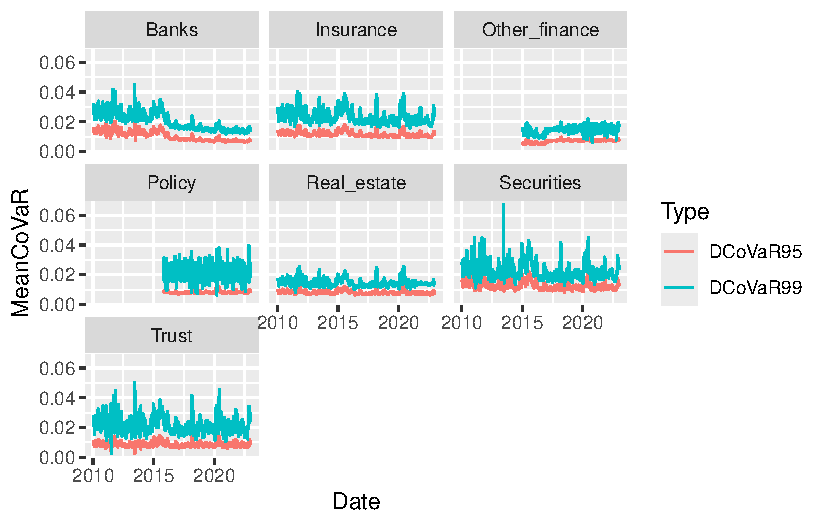
\includegraphics{chapter03-systemic_risk_files/figure-pdf/fig-CoVaRindustry-1.pdf}

}

\caption{\label{fig-CoVaRindustry}DCoVaR Visualization by Industry}

\end{figure}%

Figure~\ref{fig-CoVaRindustry} presents the individual financial
institutions' contribution to systemic risk based on industry. Based on
the visulaization, CoVaR of financial institutions in the industries of
securities and trust have higher volatility than banks, especially over
the period 2015-2022.

\begin{longtable}[]{@{}
  >{\centering\arraybackslash}p{(\columnwidth - 4\tabcolsep) * \real{0.3333}}
  >{\centering\arraybackslash}p{(\columnwidth - 4\tabcolsep) * \real{0.3333}}
  >{\centering\arraybackslash}p{(\columnwidth - 4\tabcolsep) * \real{0.3333}}@{}}

\caption{\label{tbl-regression}Regulatory Capital and Systemic Risk
Estimated}

\tabularnewline

\toprule\noalign{}
\endhead
\bottomrule\noalign{}
\endlastfoot
~ & CoVaR\_95\%CI & CoVaR\_99\%CI \\
Predictors & Estimates & Estimates \\
(Intercept) & \begin{minipage}[t]{\linewidth}\raggedright
-2.466 \textsuperscript{***}\\
(-3.055~--~-1.877)\strut
\end{minipage} & \begin{minipage}[t]{\linewidth}\raggedright
-4.389 \textsuperscript{***}\\
(-5.549~--~-3.229)\strut
\end{minipage} \\
TC RWA & \begin{minipage}[t]{\linewidth}\raggedright
-0.023 \textsuperscript{**}\\
(-0.037~--~-0.009)\strut
\end{minipage} & \begin{minipage}[t]{\linewidth}\raggedright
-0.054 \textsuperscript{***}\\
(-0.082~--~-0.027)\strut
\end{minipage} \\
LnAssets & \begin{minipage}[t]{\linewidth}\raggedright
0.172 \textsuperscript{***}\\
(0.150~--~0.194)\strut
\end{minipage} & \begin{minipage}[t]{\linewidth}\raggedright
0.283 \textsuperscript{***}\\
(0.240~--~0.327)\strut
\end{minipage} \\
NL to TA & \begin{minipage}[t]{\linewidth}\raggedright
0.004 \textsuperscript{*}\\
(0.000~--~0.007)\strut
\end{minipage} & \begin{minipage}[t]{\linewidth}\raggedright
0.013 \textsuperscript{***}\\
(0.006~--~0.020)\strut
\end{minipage} \\
Liquidity Ratio & \begin{minipage}[t]{\linewidth}\raggedright
0.011 \textsuperscript{***}\\
(0.007~--~0.016)\strut
\end{minipage} & \begin{minipage}[t]{\linewidth}\raggedright
0.031 \textsuperscript{***}\\
(0.023~--~0.039)\strut
\end{minipage} \\
Funding Ratio & \begin{minipage}[t]{\linewidth}\raggedright
-0.002 \textsuperscript{}\\
(-0.005~--~0.001)\strut
\end{minipage} & \begin{minipage}[t]{\linewidth}\raggedright
-0.001 \textsuperscript{}\\
(-0.007~--~0.004)\strut
\end{minipage} \\
Ownership {[}State-owned{]} &
\begin{minipage}[t]{\linewidth}\raggedright
0.125 \textsuperscript{**}\\
(0.037~--~0.214)\strut
\end{minipage} & \begin{minipage}[t]{\linewidth}\raggedright
0.305 \textsuperscript{***}\\
(0.131~--~0.479)\strut
\end{minipage} \\
\begin{minipage}[t]{\linewidth}\raggedright
Ownership {[}Local\\
government-holding{]}\strut
\end{minipage} & \begin{minipage}[t]{\linewidth}\raggedright
0.103 \textsuperscript{***}\\
(0.043~--~0.163)\strut
\end{minipage} & \begin{minipage}[t]{\linewidth}\raggedright
-0.005 \textsuperscript{}\\
(-0.123~--~0.113)\strut
\end{minipage} \\
\begin{minipage}[t]{\linewidth}\raggedright
Ownership {[}Foreign\\
Joint-stock{]}\strut
\end{minipage} & \begin{minipage}[t]{\linewidth}\raggedright
0.177 \textsuperscript{***}\\
(0.106~--~0.249)\strut
\end{minipage} & \begin{minipage}[t]{\linewidth}\raggedright
0.194 \textsuperscript{**}\\
(0.053~--~0.335)\strut
\end{minipage} \\
Observations & 960 & 960 \\
R\textsuperscript{2} / R\textsuperscript{2} adjusted & 0.453 / 0.448 &
0.412 / 0.407 \\
\multicolumn{3}{@{}>{\raggedleft\arraybackslash}p{(\columnwidth - 4\tabcolsep) * \real{1.0000} + 4\tabcolsep}@{}}{%
* p\textless0.05~~~** p\textless0.01~~~*** p\textless0.001} \\

\end{longtable}

Table~\ref{tbl-regression} presents the results from the regression
Equation(1) where we examine the baseline relationship between Basel III
capital adequacy regulation and systemic risk measured using CoVaR.
Based on the results of Hausman test, we employ the fixed-effect OLS
regression model to exmaine the relation between total regulatory
capital ratio and CoVaR95 (CoVaR at 95\% confidence level) and CoVaR99
(CoVaR at 99\% confidence level), respectively. We find a significant
(at 90\% confidence level) negative relationship between total
regulatory capital ratio and CoVaR. Our results are consistent with the
findings of Laeven et al. (2016) and Demirgüç-Kunt et al. (2018) that
regulatory capital is inversely related to systemic risk, and higher
levels of the regulatory capital ratio may contribute to decreasing
systemic risk.

\subsection{Bank Characteristics and Systemic
Risk}\label{bank-characteristics-and-systemic-risk}

The bank-level variables perform as expected and show consistent results
with the ones in Adrian and Brunnermeier (2016), Demirgüç-Kunt et al.
(2018) and Laeven et al. (2016). Bank size (variable \emph{LnAssets}) is
positively associated with systemic risk. Large banks usually have broad
connectedness to the entire financial system and have inclines to engage
more in risky investments such as trading. Therefore, the high maturity
mis-match ratio makes those large banks more vulnerable and generate
externalities of liquidity shocks and market faliures such as fire sale
(Boot and Ratnovski, 2012; see Shleifer and Vishny, 2010). Our results
also support the view of agency cost that large banks, because of their
engagement with complex trading, may suffer from increased agency
problems leading to build-up and generation of higher systemic risk
(Laeven and Levine, 2007). \emph{Liquidity Ratio} shows positive
relation with systemic risk. When banks have higher liquidity ratio
(i.e.~more short-term trading assets), they may be exposed to higher
illiquid risk. In financial distress, an individual bank's liquidity
shortage can be transmitted to the entire financial system through fire
sales. The positive relation holds between bank loans (variable
\emph{NL\_to\_TA}) and systemic risk. The ratio of total net loans to
total assets (\emph{NL\_to\_TA}) can be used as the proxy of an
individual bank's involvement in market-based activities (Laeven et al.,
2016). An individual bank with a lower net loan ratio may be considered
that it may be engaged with more frequent market-based activities.
Intuitively, the individual bank may be exposed to higher risk of
negative externalities that affect the whole financial system. However,
our result shows that high market-based exposures may not increase the
individual bank's contribution to systemic risk (increasing the risk of
contagion) when the bank is in financial distress.

Ownership structure of Chinese banks is always a research area that
attracts academic interests. We find that adding ownership structure
does not change the significant and negative association between the
total regulatory capital ratio and systemic risk. Berger et al. (2009)
study efficiency of Chinese banks from the perspective of ownership
structure and report that a minority of foreign ownership help improve
bank efficiency. Tan and Floros (2013) investigate the effect of capital
ratio on Chinese banks' cost efficiency adjusting for ownership
structure. The thirty years of the reform in China's banking industry
(1978-2010) achieved the advancement of the legal and financial
infrastructure, as well as the more diversified ownership structure. By
2010 the four G-SIBs and other 12 commercial banks all completed IPOs.
Private shareholding accounted for 77.7\% in rural commercial banks. The
period after 2010 could be considered as a stage of the financial reform
for further progressing and improving on both infrastructure and
ownership changes. In recent times, as China seeks to decouple its
reserve banking system from the US, there may be important implications
for continued regulatory cooperation in international
banking\footnote{\url{https://rhg.com/research/us-china-decoupling}}.

The results reveal that compared to joint-stock banks which is the base
category, state-owned banks, local government-holding banks and foreign
joint-stock banks (foreign ownership as the minority shareholder) have
higher contribution to systemic risk when individual banks are in
distress. From the perspective of standalone bank risk, our findings
support the viewpoint that state-owned banks are engaged with a number
of policy-guided credit activities which might not be profit-centered
(see Pessarossi and Weill, 2015). The social lending theory of state
ownership proposed by Atkinson and Stiglitz (1980) suggests that
state-owned enterprises contribute to ``correcting the `failure' of
market economy'' due to imperfect competition, inefficiency and public
good. Therefore, government-owned enterprises may help improve overall
performance of economy (see Stiglitz, 1993). Nevertheless, state-owned
banks may be exposed to high credit risk brought by those social welfare
projects. In China's banking context, the four of the ``Big Six'' were
founded and conducted a large amount of government lending in the early
1990's, before national banks and city banks were established. Within a
relatively long period, the state-owned banks (including local
government-holding banks founded later in the end of 1990's) played a
role of `government agencies' to pursue the broader social welfare
objectives rather than profit maximizing; for example, the projects of
the nationwide High-speed Rail network. These projects are long-term
focus, requiring patient capital and borne with high opportunity costs
and probably low profitability. According to Tirole (1994), the managers
in the state-owned banks have low powered incentives, since the
state-owned banks target multiple welfare objectives which might not be
measurable. The engagement with social welfare projects resulted in the
significant non-performing loan levels of `Big Four' banks before
China's WTO accession in 2001.

Since 2001, the ownership structure has been dramatically transformed
due to China's overall industrial reforms and the commitments to the WTO
agreement. The large part of shares directly held by local government
were gradually replaced by mixed ownership enterprises, foreign
investments, and private investors. In terms of the state-owned banks,
direct state intervention was replaced by Central Huijin (a corporate
shareholder representing the state government) along with the
establishment of modern corporate governance system. Those
infrastructure projects that purely focus on social welfare would be
taken over by the policy banks\footnote{The three policy banks, China
  Development Bank, The Export-Import Bank of China, and The
  Agricultural Development Bank of China, were founded in 1994.} or
would be financed by syndicated loans, in order to mitigate potential
downsides and remain resilient to adverse market conditions. The
state-shareholding in state-owned banks have been transformed into
concentrated ownership (see Shleifer and Vishny, 1997) but with powerful
cash flow rights. Therefore, concentrated ownership puts pressure on
management decision (Shleifer and Vishny, 1997) and bank risk taking
incentives (Boyd and Hakenes, 2008). Most of state-owned Chinese banks
are those largest banks in China's market in terms of
branches/subsidiaries and total assets. According to ``Too-big-to-fail''
view, large and complex banks tend to take excessive risk depending on
anticipated regulatory policy reaction (Farhi and Tirole, 2012). These
large and complex state-owned banks are the essential part of the whole
financial system through their diversified activities and connected the
whole financial network. Therefore, large size and the network
connectedness increase the systemic risk contribution of state-owned
banks, escalating the externalities created when they are in distress.

\section{Conclusion}\label{conclusion-3}

The global financial crisis (GFC) in 2007-2009 has demonstrated that the
capital regulations in place were not adequate to protect financial
institutions from systematic distress. Therefore, there has been
academic interest in assessing the key reforms in Basel regulation and
supervision framework. In this paper, we examine the relation between
Basel III regulatory capital ratio and systemic risk in China's banking
industry over the period 2010-2022. We find that there is negative
relation between total regulatory capital ratio and systemic risk, which
means systemic risk is lower in more-capitalized banks in China.

We also analyze the impact of bank-level variables on systemic risk.
Bank size makes positive contribution to the increase of systemic risk.
Our findings also show that high liquidity ratio imposes excessive
systemic risk, which can be considered as evidence in support of more
stringent regulations on inter-bank trading and maturity mismatch.
However, calls to regulate trading business should come with prudence
because our empirical research does not provide more detailed evidence
on optimal size of trading relative to liquid assets or total assets.

Moreover, we investigate the impact of different ownership structure on
systemic risk. Our results show that state-owned banks have higher
contribution to systemic risk than joint-stock banks. We argue that
systemic risk is influenced by the interplay of ownership structure,
bank size and diversification. The concentration of state-owned
shareholding with significant cash flow rights, coupled with the sheer
size, may amplify the systemic repercussion in times of economic stress.
Furthermore, the high level of diversification across state-owned banks'
portfolio can exacerbate systemic risk by the broad interconnectedness
of the bank in the financial system. Four of twelve state-owned banks
are G-SIBs. From this perspective, our findings underpin the importance
of regulating ``Too-big-to-fail'' financial institutions. However, more
detailed research is needed to facilitate regulations and supervision
framework.

\subsection{Discussions and Research
Directions}\label{discussions-and-research-directions}

Due to the expansion of the global financial network and the extensive
integration and interconnectedness within the global financial system,
financial stress experienced by one bank has the potential to cascade to
other banks, posing a threat to the broader financial system and
potentially triggering a global systemic crisis (Greenwood et al.,
2015). Global systemically important banks (G-SIBs), given their
significant exposure to economic shocks, primarily drive system-wide
distress. Authorities such as Financial Stability Board(FSB) finalized
the Total Loss-Absorbing Capacity(TLAC) standards to require
resolvability of G-SIBs. Our future research endeavors could entail
conducting a comparative study among emerging markets where global
systemically important banks (G-SIBs) are situated, and which share
similar macroeconomic environments. This exploration aims to broaden the
existing literature on systemic risk and provide implication for
regulators by examining how G-SIBs operate within various emerging
market contexts.

Our results may be driven by the endogeneity concerns as the level of
regulatory capital kept by banks may fluctuated when systemic risk
increasing in the financial system. We use the lagged values of
bank-level variables in order to partially alleviate the concerns in our
main analysis. Our findings may also have been influenced by the
methodology used to measure systemic risk, particularly considering
criticisms of market-based measures in the literature. Borio and
Drehmann (2009) have highlighted the limited scope of market-based
measures in capturing systemic risk adequately. Besides, while the
market-based models have demonstrated satisfactory performance within
the United States, their efficacy in other markets(e.g.~emerging
markets) may need refinement and adaptation (Arnold et al., 2012). In
our study, we utilize a market-based systemic risk measure known as
conditional value at risk (CoVaR), as proposed by Adrian and
Brunnermeier (2016). CoVaR incorporates macroeconomic data and
firm-specific characteristics, addressing some of the limitations
associated with traditional market-based measures. Consequently, CoVaR
has gained widespread acceptance as a tool for systemic risk assessment
in literature such as Laeven et al. (2016), Demirgüç-Kunt et al. (2018)
and Huang et al. (2019). However, it is important to acknowledge that
CoVaR's reliance on stock market returns may still present a limitation
in terms of its coverage. We intend to employ other alternative measures
of systemic risk such as the Marginal Expected Shortfall(MES) to gauge
banks' expected equity loss when the financial system is in distress
(see Acharya et al., 2017) in future research.

\newpage

\section{Appendix}\label{appendix-1}

\subsection{Correlation Matrix}\label{correlation-matrix}

\begin{figure}

\centering{

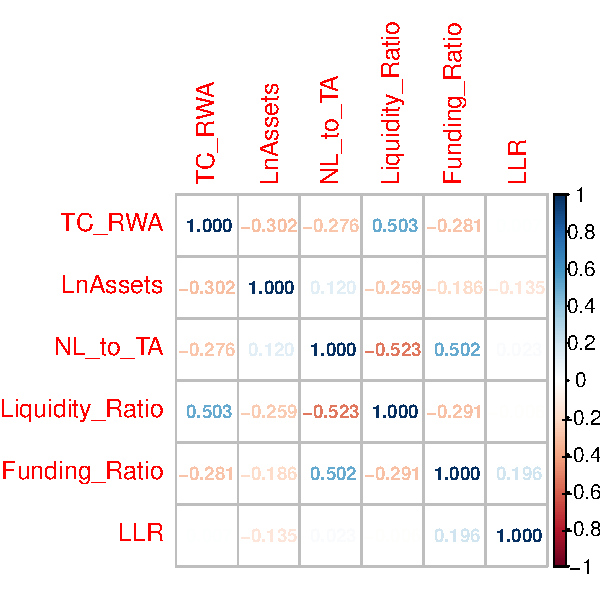
\includegraphics{chapter03-systemic_risk_files/figure-pdf/fig-appendixcorrelation-1.pdf}

}

\caption{\label{fig-appendixcorrelation}Linear Correlation Matrix}

\end{figure}%

\bookmarksetup{startatroot}

\chapter{Conclusion}\label{conclusion-4}

\section{Research Summary}\label{research-summary}

My thesis explores the interplay between Basel III capital adequacy
regulation and risk-taking, efficiency, and systemic stability within
the Chinese banking industry, with a specific focus on the influence of
ownership structure. The objectives were to analyze the impact of Basel
III capital regulation on bank credit risk, cost efficiency and
stability of the whole financial system, and to assess the influence of
different ownership structure in the Chinese context. The 2007-2009
Global Financial Crisis (GFC) uncovered that the pre-crisis capital
regulations have structural weaknesses and were not adequate to protect
financial institutions from systemic distress. The Basel Committee on
Banking Regulation and Supervision (BCBS) developed a consolidated
framework (Basel III) for more stringent capital adequacy regulations.
There is continued academic interest on the effect of implementation of
Basel III capital requirements (see Demirguc-Kunt et al., 2013), despite
the regulatory consensus. This thesis reveals nuanced insights that
contribute significantly to our understanding of the interplay between
regulatory framework, ownership structures, and the broader financial
stability landscape.

Since 1978, the Chinese banking sector has been reformed as part of the
country's overall economic reform. After forty years, Chinese banks
actively participate in global financial markets as influential players
and contribute to the interconnectedness of the international financial
system. Chapter 2 provides a review of China's banking landscape
including the evolution of the financial reforms, the regulatory
framework and the essential financial indicators. The objectives of
Chapter 2 were to understand the unique context of China's banking
industry, the adherence to the Basel III framework, and the Chinese
banks' presence in and interconnectedness to global financial system,
thereby offering research background for the following chapters of
empirical analyses. The review shows that the reform and legislative
advancements in China's banking sector, coupled with transformation
initiatives, have resulted in diversified ownership structure,
contemporary corporate governance frameworks, and heightened market
competition. The active intervention of the government appears to be
progressively receding with each phase of reform.The Basel III framework
has been fully adopted and incorporated into the banking regulatory
framework in China \footnote{China fully adopted Basel III in 2012,
  after adopted and implemented Basel II and Basel II.5 in previous
  years.}. Employing the CAMELS rating system, Chapter 2 assesses the
safety and soundness of Chinese banks. In summary, China's commercial
banks exhibit robust capital adequacy, surpassing the Basel III standard
with a ratio exceeding 10\%, and maintain a lower average NPL ratio
compared to G20 peers. However, our analysis highlights potential
vulnerabilities for small and medium banks facing elevated credit risks,
suggesting a need for enhanced safeguards. Notably, Chinese commercial
banks demonstrate a competitive edge with lower cost-to-income ratios
and an average return on equity exceeding 14\%. While liquidity risk is
generally well-managed in the biggest and those small-sized banks,
medium-sized banks, particularly those historically linked to local
government shareholders, may face higher liquidity risks due to
increased reliance on wholesale funding channels.

Chapter 3, our initial investigation builds upon previous empirical
studies that examine how Basel III risk-based capital requirements
influence banks' credit risk-taking. We enhance our research by
considering the interplay between capital regulation and ownership
structure. This study employs forensically analyzed data on 231 Chinese
banks over the period 2010-2019. The negative impact on bank credit
risk-taking suggests that the implementation of Basel III has indeed
fortified financial stability. Notably, state-owned banks emerge as key
players in this dynamic, exhibiting higher credit risk-taking compared
to other ownership structures. This finding is consistent with the
results of Zhu and Yang (2016) and to some extent, echo the empirical
results of Laeven and Levine (2009), indicating that banks with large
shareholders holding substantial cash flow rights tend to assume greater
credit risk. Our findings also align with the social perspective of the
theory of state ownership of banks (see Stiglitz, 1993), indicating that
state-owned banks are inclined to undertake credit projects even if they
may not be financially profitable. Moreover, this study provides new
evidence that the influence of Basel III capital regulation on credit
risk-taking is, to some extent, contingent on ownership structure. This
result reinforce the empirical conclusion drawn by Laeven and Levine
(2009).

Efficiency analysis forms the core of Chapter 4, unraveling the nuanced
components of transient and persistent efficiency, which contributes
granularity to our comprehension of the efficiency dynamics with China's
banking sector. Our empirical research provides evidence using a
four-component panel stochastic frontier cost model on an unbalanced
panel of 233 China's commercial banks over the period 2010-2020. A key
finding of this chapter is the distinctive profile exhibited by
state-owned banks in terms of efficiency.The results provide that
state-owned banks have higher transient efficiency and much lower
persistent efficiency compared with other ownership types, which
collaborate the findings by Fungáčová et al. (2020). We do not find
statistically significant relation between the regulatory capital
requirements and persistent cost efficiency but a negative relation
between regulatory capital and transient efficiency.This result supports
the findings of some empirical literature (see Barth et al., 2004;
Djalilov and Piesse, 2019; Lee and Chih, 2013; Lešanovská and Weill,
2016), however differs from other previous studies. The intricate
relationship between ownership structure and bank cost efficiency is
statistically significant. We provide the explanation for state-owned
banks' relatively low persistent efficiency and high transient
efficiency, compared with other ownership.

Efficiency analysis in Chapter 4 sheds light on broader banking dynamics
by adding a layer of complexity to the understanding of the regulatory
impact of Basel III framework. In particular, the findings refines our
understanding of state-owned banks by introducing the distinctive
efficiency profile of state-owned banks.

Chapter 5 delves into the complex realm of Basel III regulatory capital
ratios and systemic risk. We collect data of 376 Chinese financial
institutions including 236 banks over the period of 2010-2022, and
compute the conditional value at risk (CoVaR) proposed by Adrian and
Brunnermeier (2016) as the measure of systemic risk. This study
establishes a negative relation between total regulatory capital ratio
and systemic risk, signaling a pivotal role of Basel III risk-based
capital adequacy requirements in enhancing financial stability. Our
finding aligns and corroborate the previous empirical results (see
Demirgüç-Kunt et al., 2018; Laeven et al., 2016). Bank size is
identified as a positive contributor to systemic risk, while a high
liquidity ratio emerges as a potential source of excessive systemic
risk, emphasizing the necessity for more stringent regulations.
Importantly, the examination of ownership structures highlights
state-owned banks as significant contributors to systemic risk,
reinforcing the importance of regulating ``Too-big-to-fail'' financial
institutions. The intricate interplay of ownership structure, bank size,
and diversification is unveiled as a crucial determinant of systemic
risk in times of economic stress.

Chapter 5, our final empirical chapter serves as a crucial piece of the
overall narrative, relating and expanding the insights gleaned from the
first two studies. This chapter further solidifies that Basel III
capital regulation enhance overall financial stability by establishing a
negative relation between total regulatory capital ratio and systemic
risk. The bank efficiency considerations are incorporated into the
broader context of systemic stability, demonstrating that efficiency
dynamics are integral to understanding the potential systemic
repercussion of different ownership structure. The empirical results
from the three chapters contribute to a holistic understanding of the
determinants of systemic risk. The interplay of Basel III capital
regulations, ownership structure, efficiency dynamics, and risk
dimensions provides a comprehensive view of the factors influencing
financial stability under the context of China's banking sector.

\subsection{Contribution}\label{contribution}

Based on the research that was investigated, this thesis contributes to
the understanding of China's banking industry by exploring dimensions
related to Basel III capital regulations, efficiency components and
systemic stability. The study holds importance to policy-making as it
aligns with the Basel Committee on Banking Supervision's (BCBS)
post-crisis reform initiative, as well as addresses fostering global
financial stability, by evaluating the influence of Basel III risk-based
capital regulations on individual bank risk-taking and overall systemic
risk in China's banking system given China's significant role in the
global financial system. The research bridges a gap by examining the
joint effects of ownership structure and Basel III capital requirements
on bank credit risk-taking. Existing studies rarely explore this
interaction, making this research valuable in understanding how
ownership structure and regulatory measures collectively shape
risk-taking behavior in Chinese banks. The study also contributes to
literature by analyzing how ownership structure influences efficiency
and financial stability, offering insights into moral hazard factors and
designing targeted regulatory measures. The study addresses a gap in
literature by focusing on the systemic risk within China's banking
sector which is a relatively under-explored area, particularly post the
implementation of Basel III in China.

\subsection{Limitations}\label{limitations}

This thesis has limitations that should be addressed:

\subsubsection{Data Qualitiy and
Availability}\label{data-qualitiy-and-availability}

The accuracy and comprehensiveness of the findings depend on the quality
and availability of the data used. The data provided by our main data
source - the SNL Capital Pro database have been supplemented by manually
collected data from other official data sources such as the China
Banking and Insurance Regulatory Commission (CBIRC), and the annual
reports of individual banks. Incomplete data could be a limitation that
affects the study's robustness.

\subsubsection{Model Limitation}\label{model-limitation}

The efficiency study employs a three-step, four component stochastic
frontier model may introduce complexity and high demands on data and
computation, which could affect the accuracy of empirical results.

CoVaR is employed in Chapter 5 as a measure of systemic risk. However,
this measure has been criticized not fully capturing externalities such
as contagion, fire sales or spillover effects (see Demirgüç-Kunt et al.,
2018), and might need to be complemented by other metrics such as
Marginal Expected Shortfall (MES) to obtain a comprehensive view of
systemic risk.

\subsubsection{External Factors}\label{external-factors}

The study may not account for all external factors that could influence
the observed relationships. Economic, geopolitical, or regulatory
changes not considered in the research could impact the results, for
example, the input and output variables for measuring the level of bank
efficiency might not be exhaustive.

\bookmarksetup{startatroot}

\chapter*{Bibliography}\label{bibliography}
\addcontentsline{toc}{chapter}{Bibliography}

\markboth{Bibliography}{Bibliography}

\phantomsection\label{refs}
\begin{CSLReferences}{1}{0}
\bibitem[\citeproctext]{ref-BCBS2018_about}
\href{https://www.bis.org/bcbs/about/overview.htm?m=85}{About the BCBS},
2018. www.bis.org.

\bibitem[\citeproctext]{ref-ACHARYA2009}
Acharya, V.V., 2009. A theory of systemic risk and design of prudential
bank regulation. Journal of Financial Stability 5, 224--255.
https://doi.org/\url{https://doi.org/10.1016/j.jfs.2009.02.001}

\bibitem[\citeproctext]{ref-ACHARYA2016}
Acharya, V.V., Mehran, H., Thakor, A.V., 2016. Caught between scylla and
charybdis? Regulating bank leverage when there is rent seeking and risk
shifting. The Review of Corporate Finance Studies 5, 36--75.
\url{https://doi.org/10.1093/rcfs/cfv006}

\bibitem[\citeproctext]{ref-ACHARYA2017}
Acharya, V.V., Pedersen, L.H., Philippon, T., Richardson, M., 2017.
Measuring systemic risk. The Review of Financial Studies 30, 2--47.
\url{https://doi.org/10.1093/rfs/hhw088}

\bibitem[\citeproctext]{ref-ADMATI2014}
Admati, A.R., DeMarzo, P.M., Hellwig, M.F., Pfleiderer, P., 2014.
\href{http://www.jstor.org/stable/j.ctt1gxpd6m.6}{FALLACIES AND
IRRELEVANT FACTS IN THE DISCUSSION ON CAPITAL REGULATION}, in: Goodhart,
C., Gabor, D., Vestergaard, J., Ertürk, I. (Eds.), Central Banking at a
Crossroads, Europe and Beyond. Anthem Press, pp. 33--50.

\bibitem[\citeproctext]{ref-ADRIAN2016}
Adrian, T., Brunnermeier, M.K., 2016.
\href{http://www.jstor.org/stable/43861110}{CoVaR}. The American
Economic Review 106, 1705--1741.

\bibitem[\citeproctext]{ref-AIGNER1977}
Aigner, D., Lovell, C.A.K., Schmidt, P., 1977. Formulation and
estimation of stochastic frontier production function models. Journal of
Econometrics 6, 21--37.
https://doi.org/\url{https://doi.org/10.1016/0304-4076(77)90052-5}

\bibitem[\citeproctext]{ref-ALCHIAN1965}
Alchian, A.A., 1965. \href{http://www.jstor.org/stable/43206327}{SOME
ECONOMICS OF PROPERTY RIGHTS}. Il Politico 30, 816--829.

\bibitem[\citeproctext]{ref-ALCHIAN1972}
Alchian, A.A., Demsetz, H., 1972.
\href{http://www.jstor.org/stable/1815199}{Production, information
costs, and economic organization}. The American Economic Review 62,
777--795.

\bibitem[\citeproctext]{ref-ALLEN2011}
Allen, F., Carletti, E., Marquez, R., 2011.
\href{http://www.jstor.org.queens.ezp1.qub.ac.uk/stable/20869263}{Credit
market competition and capital regulation}. The Review of Financial
Studies 24, 983--1018.

\bibitem[\citeproctext]{ref-ALLEN2000}
Allen, F., Gale, D., 2000. Financial contagion. Journal of Political
Economy 108, 1--33. \url{https://doi.org/10.1086/262109}

\bibitem[\citeproctext]{ref-ALTUNBAS2007}
Altunbas, Y., Carbo, S., Gardener, E.P.M., Molyneux, P., 2007. Examining
the relationships between capital, risk and efficiency in european
banking. European Financial Management 13, 49--70.
https://doi.org/\url{https://doi.org/10.1111/j.1468-036X.2006.00285.x}

\bibitem[\citeproctext]{ref-ALTUNBAS2001}
Altunbas, Y., Evans, L., Molyneux, P., 2001. Bank ownership and
efficiency. Journal of Money, Credit and Banking 33, 926--954.
\url{https://doi.org/10.2307/2673929}

\bibitem[\citeproctext]{ref-AMIHUD1981}
Amihud, Y., Lev, B., 1981. Risk reduction as a managerial motive for
conglomerate mergers. The Bell Journal of Economics 12, 605--617.
\url{https://doi.org/10.2307/3003575}

\bibitem[\citeproctext]{ref-ANDRIANOVA2012}
Andrianova, S., Demetriades, P., Shortland, A., 2012.
\href{http://www.jstor.org/stable/23274805}{Government ownership of
banks, institutions and economic growth}. Economica 79, 449--469.

\bibitem[\citeproctext]{ref-ANGINER2021}
Anginer, D., Bertay, A.C., Cull, R., Demirgüç-Kunt, A., Mare, D.S.,
2021. Bank capital regulation and risk after the global financial
crisis. Journal of Financial Stability.
\url{https://doi.org/10.1016/j.jfs.2021.100891}

\bibitem[\citeproctext]{ref-ANGINER2014}
Anginer, D., Demirguc-Kunt, A., 2014. Bank capital and systemic
stability. Policy Research Working Papers 6948, 42.
\url{https://doi.org/doi:10.1596/1813-9450-6948}

\bibitem[\citeproctext]{ref-ARENA2008}
Arena, M., 2008. Bank failures and bank fundamentals: A comparative
analysis of latin america and east asia during the nineties using
bank-level data. Journal of Banking \& Finance 32, 299--310.
https://doi.org/\url{https://doi.org/10.1016/j.jbankfin.2007.03.011}

\bibitem[\citeproctext]{ref-ARNOLD2012}
Arnold, B., Borio, C., Ellis, L., Moshirian, F., 2012. Systemic risk,
macroprudential policy frameworks, monitoring financial systems and the
evolution of capital adequacy. Journal of Banking \& Finance 36,
3125--3132.
https://doi.org/\url{https://doi.org/10.1016/j.jbankfin.2012.07.023}

\bibitem[\citeproctext]{ref-ATHERTON2016}
Atherton, A., Newman, A., 2016. The emergence of the private
entrepreneur in reform era china: Re-birth of an earlier tradition, or a
more recent product of development and change? Business History 58,
319--344. \url{https://doi.org/10.1080/00076791.2015.1122702}

\bibitem[\citeproctext]{ref-ATKINSON1980}
Atkinson, Anthony.B., Stiglitz, Joseph.E., 1980. Lectures on public
economics. McGraw-Hill Book Co, London ; New York.

\bibitem[\citeproctext]{ref-AYADI2020}
Ayadi, R., Bongini, P., Casu, B., Cucinelli, D., 2020. Bank business
model migrations in europe: Determinants and effects. British Journal of
Management n/a.
https://doi.org/\url{https://doi.org/10.1111/1467-8551.12437}

\bibitem[\citeproctext]{ref-BADUNENKO2017}
Badunenko, O., Kumbhakar, S.C., 2017. Economies of scale, technical
change and persistent and time-varying cost efficiency in indian
banking: Do ownership, regulation and heterogeneity matter? European
Journal of Operational Research 260, 789--803.
https://doi.org/\url{https://doi.org/10.1016/j.ejor.2017.01.025}

\bibitem[\citeproctext]{ref-BAI2020}
Bai, H., Ba, S., Huang, W., Hu, W., 2020. Expected government support
and bank risk-taking: Evidence from china. Finance Research Letters 36,
101328. https://doi.org/\url{https://doi.org/10.1016/j.frl.2019.101328}

\bibitem[\citeproctext]{ref-BCBS2014}
Banking Supervision, B.C. on, 2014. Implementation of basel standards -
a report to G20 leaders on implementation of the basel III regulatory
reforms (Report).
https://doi.org/\url{https://www.bis.org/bcbs/publ/d299.pdf}

\bibitem[\citeproctext]{ref-BARTH2008}
Barth, J.R., Caprio, G., Levine, R., 2008. Bank regulations are
changing: For better or worse? Comparative Economic Studies 50,
537--563. https://doi.org/\url{http://dx.doi.org/10.1057/ces.2008.33}

\bibitem[\citeproctext]{ref-BARTH2005}
Barth, J.R., Caprio, G., Levine, R., 2005. Rethinking bank regulation:
Till angels govern. Cambridge University Press, Cambridge.
\href{https://doi.org/DOI:\%2010.1017/CBO9780511753817}{https://doi.org/DOI:
10.1017/CBO9780511753817}

\bibitem[\citeproctext]{ref-BARTH2004}
Barth, J.R., Caprio, G., Levine, R., 2004. Bank regulation and
supervision: What works best? Journal of Financial Intermediation 13,
205--248.
https://doi.org/\url{https://doi.org/10.1016/j.jfi.2003.06.002}

\bibitem[\citeproctext]{ref-BARTH2013}
Barth, J.R., Lin, C., Ma, Y., Seade, J., Song, F.M., 2013. Do bank
regulation, supervision and monitoring enhance or impede bank
efficiency? Journal of Banking \& Finance 37, 2879--2892.
https://doi.org/\url{https://doi.org/10.1016/j.jbankfin.2013.04.030}

\bibitem[\citeproctext]{ref-BATTESE1995}
Battese, G.E., Coelli, T.J., 1995. A model for technical inefficiency
effects in a stochastic frontier production function for panel data.
Empirical Economics 20, 325--332.
\url{https://doi.org/10.1007/BF01205442}

\bibitem[\citeproctext]{ref-BATTESE1992}
Battese, G.E., Coelli, T.J., 1992.
\href{http://www.jstor.org/stable/41770578}{Frontier production
functions, technical efficiency and panel data: With application to
paddy farmers in india}. Journal of Productivity Analysis 3, 153--169.

\bibitem[\citeproctext]{ref-BATTESE1988}
Battese, G.E., Coelli, T.J., 1988. Prediction of firm-level technical
efficiencies with a generalized frontier production function and panel
data. Journal of Econometrics 38, 387--399.
https://doi.org/\url{https://doi.org/10.1016/0304-4076(88)90053-X}

\bibitem[\citeproctext]{ref-BAUER1993}
Bauer, P.W., Berger, A.N., Humphrey, D.B., 1993. Efficiency and
productivity growth in US banking, in: The Measurement of Productive
Efficiency: Techniques and Applications. pp. 386--413.

\bibitem[\citeproctext]{ref-BCBS2013}
BCBS, 2013. Regulatory consistency assessment programme (RCAP)
assessment of basel III regulations - china (Report). Basel Committee on
Banking Supervision.

\bibitem[\citeproctext]{ref-BEBCHUK1999}
Bebchuk, L.A., 1999. A rent-protection theory of corporate ownership and
control. Law \& Economics eJournal.

\bibitem[\citeproctext]{ref-BECK2006}
Beck, T., Demirgüç-Kunt, A., Levine, R., 2006. Bank supervision and
corruption in lending. Journal of Monetary Economics 53, 2131--2163.
https://doi.org/\url{https://doi.org/10.1016/j.jmoneco.2005.10.014}

\bibitem[\citeproctext]{ref-BECK2004}
Beck, T., Demirgüç-Kunt, A., Maksimovic, V., 2004.
\href{http://www.jstor.org.queens.ezp1.qub.ac.uk/stable/3838958}{Bank
competition and access to finance: International evidence}. Journal of
Money, Credit and Banking 36, 627--648.

\bibitem[\citeproctext]{ref-BECK2002}
Beck, T., Levine, R., 2002. Industry growth and capital allocation::
Does having a market- or bank-based system matter? Journal of Financial
Economics 64, 147--180.
https://doi.org/\url{https://doi.org/10.1016/S0304-405X(02)00074-0}

\bibitem[\citeproctext]{ref-BELLAVITE-PELLEGRINI2022}
Bellavite Pellegrini, C., Cincinelli, P., Meoli, M., Urga, G., 2022. The
contribution of (shadow) banks and real estate to systemic risk in
china. Journal of Financial Stability 60, 101018.
https://doi.org/\url{https://doi.org/10.1016/j.jfs.2022.101018}

\bibitem[\citeproctext]{ref-BERGER2013}
Berger, A.N., Bouwman, C.H.S., 2013. How does capital affect bank
performance during financial crises? Journal of Financial Economics 109,
146--176.
https://doi.org/\url{https://doi.org/10.1016/j.jfineco.2013.02.008}

\bibitem[\citeproctext]{ref-BERGER2005}
Berger, A.N., Clarke, G.R.G., Cull, R., Klapper, L., Udell, G.F., 2005.
Corporate governance and bank performance: A joint analysis of the
static, selection, and dynamic effects of domestic, foreign, and state
ownership. Journal of Banking \& Finance 29, 2179--2221.
https://doi.org/\url{https://doi.org/10.1016/j.jbankfin.2005.03.013}

\bibitem[\citeproctext]{ref-BERGER2010}
Berger, A.N., Hasan, I., Zhou, M., 2010. The effects of focus versus
diversification on bank performance: Evidence from chinese banks.
Journal of Banking \& Finance 34, 1417--1435.
https://doi.org/\url{https://doi.org/10.1016/j.jbankfin.2010.01.010}

\bibitem[\citeproctext]{ref-BERGER2009}
Berger, A.N., Hasan, I., Zhou, M., 2009. Bank ownership and efficiency
in china: What will happen in the world's largest nation? Journal of
Banking \& Finance 33, 113--130.
https://doi.org/\url{https://doi.org/10.1016/j.jbankfin.2007.05.016}

\bibitem[\citeproctext]{ref-BERGER1995}
Berger, A.N., Herring, R.J., Szegö, G.P., 1995. The role of capital in
financial institutions. Journal of Banking \& Finance 19, 393--430.
https://doi.org/\url{https://doi.org/10.1016/0378-4266(95)00002-X}

\bibitem[\citeproctext]{ref-BERGER1997}
Berger, A.N., Humphrey, D.B., 1997. Efficiency of financial
institutions: International survey and directions for future research.
European Journal of Operational Research 98, 175--212.
https://doi.org/\url{https://doi.org/10.1016/S0377-2217(96)00342-6}

\bibitem[\citeproctext]{ref-BERGER1991}
Berger, A.N., Humphrey, D.B., 1991. The dominance of inefficiencies over
scale and product mix economies in banking. Journal of Monetary
Economics 28, 117--148.
https://doi.org/\url{https://doi.org/10.1016/0304-3932(91)90027-L}

\bibitem[\citeproctext]{ref-BERGER2019}
Berger, A.N., Molyneux, P., S., W.J.O., 2019. The oxford handbook of
banking. Oxford University Press.
\url{https://doi.org/10.1093/oxfordhb/9780198824633.001.0001}

\bibitem[\citeproctext]{ref-BERLE1932}
Berle, A.A., Means, G.C.(Gardiner.C., 1932. The modern corporation and
private property. Macmillan, New York.

\bibitem[\citeproctext]{ref-BHATTACHARYA1998}
Bhattacharya, S., Arnoud, W.A.B., Thakor, A.V., 1998. The economics of
bank regulation. Journal of Money, Credit and Banking 30, 745--770.
\url{https://doi.org/10.2307/2601127}

\bibitem[\citeproctext]{ref-BHATTACHARYA1993}
Bhattacharya, S., Thakor, A.V., 1993. Contemporary banking theory.
Journal of Financial Intermediation 3, 2--50.
https://doi.org/\url{https://doi.org/10.1006/jfin.1993.1001}

\bibitem[\citeproctext]{ref-BIERTH2015}
Bierth, C., Irresberger, F., Weiß, G.N.F., 2015. Systemic risk of
insurers around the globe. Journal of Banking \& Finance 55, 232--245.
https://doi.org/\url{https://doi.org/10.1016/j.jbankfin.2015.02.014}

\bibitem[\citeproctext]{ref-BITAR2018}
Bitar, M., Pukthuanthong, K., Walker, T., 2018. The effect of capital
ratios on the risk, efficiency and profitability of banks: Evidence from
OECD countries. Journal of International Financial Markets, Institutions
and Money 53, 227--262.
https://doi.org/\url{https://doi.org/10.1016/j.intfin.2017.12.002}

\bibitem[\citeproctext]{ref-BLUM1999}
Blum, J., 1999. Do capital adequacy requirements reduce risks in
banking? Journal of Banking \& Finance 23, 755--771.
https://doi.org/\url{https://doi.org/10.1016/S0378-4266(98)00113-7}

\bibitem[\citeproctext]{ref-BOOT2012}
Boot, A.W.A., Ratnovski, L., 2012. Banking and trading. IMF Working
Papers 2012, 48.
https://doi.org/\url{https://doi.org/10.5089/9781475511215.001}

\bibitem[\citeproctext]{ref-BORIO2003}
Borio, C.E.V., 2003. Towards a macroprudential framework for financial
supervision and regulation? / by claudio borio, BIS working papers,
1020-0959 ; no. 128. Bank for International Settlements, Monetary;
Economic Dept, Basle.

\bibitem[\citeproctext]{ref-BORIO2009}
Borio, C.E.V., Drehmann, M., 2009. {Towards an Operational Framework for
Financial Stability: \&quot;Fuzzy\&quot; Measurement and its
Consequences} (BIS Working Paper No. 284 No. 284). Central Bank of
Chile. https://doi.org/\url{http://dx.doi.org/10.2139/ssrn.1458294}

\bibitem[\citeproctext]{ref-BOYD2008}
Boyd, J., Hakenes, H., 2008. Looting and gambling in banking crises.
SSRN Electronic Journal. \url{https://doi.org/10.2139/ssrn.1099566}

\bibitem[\citeproctext]{ref-BOYD2005}
Boyd, J.H., De Nicoló, G., 2005.
\href{http://www.jstor.org.queens.ezp1.qub.ac.uk/stable/3694928}{The
theory of bank risk taking and competition revisited}. The Journal of
Finance 60, 1329--1343.

\bibitem[\citeproctext]{ref-BRUNNERMEIER2009}
Brunnermeier, M., Crockett, A., Goodhart, C.A., Persaud, A., Shin, H.S.,
2009. The fundamental principles of financial regulation. ICMB,
Internat. Center for Monetary; Banking Studies Geneva.

\bibitem[\citeproctext]{ref-BURKART2003}
Burkart, M., Panunzi, F., Shleifer, A., 2003.
\href{http://www.jstor.org/stable/3648187}{Family firms}. The Journal of
Finance 58, 2167--2201.

\bibitem[\citeproctext]{ref-BUSER1981}
Buser, S.A., Chen, A.H., Kane, E.J., 1981. Federal deposit insurance,
regulatory policy, and optimal bank capital. The Journal of Finance 36,
51--60. \url{https://doi.org/10.2307/2327463}

\bibitem[\citeproctext]{ref-CALEM1999}
Calem, P., Rob, R., 1999. The impact of capital-based regulation on bank
risk-taking. Journal of Financial Intermediation 8, 317--352.
https://doi.org/\url{https://doi.org/10.1006/jfin.1999.0276}

\bibitem[\citeproctext]{ref-CALOMIRIS1991}
Calomiris, C.W., Kahn, C.M., 1991.
\href{http://www.jstor.org/stable/2006515}{The role of demandable debt
in structuring optimal banking arrangements}. The American Economic
Review 81, 497--513.

\bibitem[\citeproctext]{ref-CANNAN1921}
Cannan, E., Pigou, A.C., 1921. The economics of welfare. The Economic
Journal 31, 206--213. \url{https://doi.org/10.2307/2222816}

\bibitem[\citeproctext]{ref-CHEN1999}
Chen, Y., 1999. Banking panics: The role of the first-come, first-served
rule and information externalities. Journal of Political Economy 107,
946--968. \url{https://doi.org/10.1086/250086}

\bibitem[\citeproctext]{ref-CHIARAMONTE2017}
Chiaramonte, L., Casu, B., 2017. Capital and liquidity ratios and
financial distress. Evidence from the european banking industry. The
British Accounting Review 49, 138--161.
https://doi.org/\url{https://doi.org/10.1016/j.bar.2016.04.001}

\bibitem[\citeproctext]{ref-CHORTAREAS2012}
Chortareas, G.E., Girardone, C., Ventouri, A., 2012. Bank supervision,
regulation, and efficiency: Evidence from the european union. Journal of
Financial Stability 8, 292--302.
https://doi.org/\url{https://doi.org/10.1016/j.jfs.2011.12.001}

\bibitem[\citeproctext]{ref-COASE1937}
Coase, R.H., 1937. The nature of the firm. Economica 4, 386--405.
https://doi.org/\url{https://doi.org/10.1111/j.1468-0335.1937.tb00002.x}

\bibitem[\citeproctext]{ref-COLOMBI2014}
Colombi, R., Kumbhakar, S.C., Martini, G., Vittadini, G., 2014.
Closed-skew normality in stochastic frontiers with individual effects
and long/short-run efficiency. Journal of Productivity Analysis 42,
123--136. \url{https://doi.org/10.1007/s11123-014-0386-y}

\bibitem[\citeproctext]{ref-COLOMBI2017}
Colombi, R., Martini, G., Vittadini, G., 2017. Determinants of transient
and persistent hospital efficiency: The case of italy. Health Economics
26, 5--22. https://doi.org/\url{https://doi.org/10.1002/hec.3557}

\bibitem[\citeproctext]{ref-COLOMBI2011}
Colombi, R., Martini, G., Vittadini, G., 2011.
\href{https://EconPapers.repec.org/RePEc:brh:wpaper:1101}{A stochastic
frontier model with short-run and long-run inefficiency random effects}
(Report). Department of Economics; Technology Management, University of
Bergamo.

\bibitem[\citeproctext]{ref-COOPER2002}
Cooper, R., Ross, T.W., 2002.
\href{http://www.jstor.org.queens.ezp1.qub.ac.uk/stable/827056}{Bank
runs: Deposit insurance and capital requirements}. International
Economic Review 43, 55--72.

\bibitem[\citeproctext]{ref-CORNWELL1990}
Cornwell, C., Schmidt, P., Sickles, R.C., 1990. Production frontiers
with cross-sectional and time-series variation in efficiency levels.
Journal of Econometrics 46, 185--200.
https://doi.org/\url{https://doi.org/10.1016/0304-4076(90)90054-W}

\bibitem[\citeproctext]{ref-DAGHER2016}
Dagher, J., Dell'Ariccia, G., Laeven, L., Ratnovski, L., Tong, H., 2016.
Benefits and costs of bank capital. Staff Discussion Notes 2016, A001.
\url{https://doi.org/10.5089/9781498387712.006.A001}

\bibitem[\citeproctext]{ref-DAVYDOV2021}
Davydov, D., Vähämaa, S., Yasar, S., 2021. Bank liquidity creation and
systemic risk. Journal of Banking \& Finance 123, 106031.
https://doi.org/\url{https://doi.org/10.1016/j.jbankfin.2020.106031}

\bibitem[\citeproctext]{ref-DE-ALESSI1980}
De Alessi, L., 1980. The economics of property rights: A review of the
evidence. Rsch. in L. \& Econ. 2, 1.

\bibitem[\citeproctext]{ref-DE-ALESSI1974}
De Alessi, L., 1974.
\href{https://queens.ezp1.qub.ac.uk/login?url=https://www.proquest.com/scholarly-journals/economic-analysis-government-ownership-regulation/docview/236987376/se-2?accountid=13374\%0Ahttps://resolver.ebscohost.com/openurl?ctx_ver=Z39.88-2004&ctx_enc=info:ofi/enc:UTF-8&rfr_id=info:sid/ProQ\%3Aabiglobal&rft_val_fmt=info:ofi/fmt:kev:mtx:journal&rft.genre=unknown&rft.jtitle=Public+Choice+\%28pre-1986\%29&rft.atitle=AN+ECONOMIC+ANALYSIS+OF+GOVERNMENT+OWNERSHIP+AND+REGULATION\%3A+THEORY+AND+THE+EVIDENCE+FROM+THE+ELECTRIC+POWER+INDUSTRY&rft.au=De+Alessi\%2C+Louis&rft.aulast=De+Alessi&rft.aufirst=Louis&rft.date=1974-10-01&rft.volume=19&rft.issue=&rft.spage=1&rft.isbn=&rft.btitle=&rft.title=Public+Choice+\%28pre-1986\%29&rft.issn=00485829&rft_id=info:doi/}{AN
ECONOMIC ANALYSIS OF GOVERNMENT OWNERSHIP AND REGULATION: THEORY AND THE
EVIDENCE FROM THE ELECTRIC POWER INDUSTRY}. Public Choice (pre-1986) 19,
1.

\bibitem[\citeproctext]{ref-DE-ANGELO2013}
De Angelo, H., Stulz, R.M., 2013. Why high leverage is optimal for banks
(Working Paper No. 19139), Working paper series. National Bureau of
Economic Research. \url{https://doi.org/10.3386/w19139}

\bibitem[\citeproctext]{ref-DE-BANDT2019}
De Bandt, O., Hartmann, P., 2019. Systemic risk in banking after the
great financial crisis.
\url{https://doi.org/10.1093/oxfordhb/9780198824633.013.27}

\bibitem[\citeproctext]{ref-DEMIRGUC-KUNT1997}
Demirguc-Kunt, A., Detragiache, E., 1997. The determinants of banking
crises : Evidence from industrial and developing countries. Policy
research working papers.

\bibitem[\citeproctext]{ref-DEMIRGUC-KUNT2013}
Demirguc-Kunt, A., Detragiache, E., Merrouche, O., 2013.
\href{http://www.jstor.org.queens.ezp1.qub.ac.uk/stable/23463595}{Bank
capital: Lessons from the financial crisis}. Journal of Money, Credit
and Banking 45, 1147--1164.

\bibitem[\citeproctext]{ref-DEMIRGUC-KUNT2002}
Demirguc-Kunt, A., Kane, E., 2002. Deposit insurance around the globe:
Where does it work? Journal of Economic Perspectives 16, 175--195.
\url{https://doi.org/10.1257/0895330027319}

\bibitem[\citeproctext]{ref-DEMIRGUC-KUNT2018}
Demirgüç-Kunt, A., Anginer, D., Mare, D.S., 2018. Bank capital,
institutional environment and systemic stability. Journal of Financial
Stability 37, 97--106.
https://doi.org/\url{https://doi.org/10.1016/j.jfs.2018.06.001}

\bibitem[\citeproctext]{ref-DEMIRGUC-KUNT2010}
Demirgüç-Kunt, A., Huizinga, H., 2010. Bank activity and funding
strategies: The impact on risk and returns. Journal of Financial
Economics 98, 626--650.
https://doi.org/\url{https://doi.org/10.1016/j.jfineco.2010.06.004}

\bibitem[\citeproctext]{ref-DEMSETZ1966}
Demsetz, H., 1966. \href{http://www.jstor.org/stable/724993}{Some
aspects of property rights}. The Journal of Law \& Economics 9, 61--70.

\bibitem[\citeproctext]{ref-DEMSETZ1985}
Demsetz, H., Lehn, K., 1985.
\href{http://www.jstor.org/stable/1833178}{The structure of corporate
ownership: Causes and consequences}. Journal of Political Economy 93,
1155--1177.

\bibitem[\citeproctext]{ref-DIAMOND1984}
Diamond, D.W., 1984. Financial intermediation and delegated monitoring.
Review of Economic Studies 51, 393.
\url{https://doi.org/10.2307/2297430}

\bibitem[\citeproctext]{ref-DIAMOND1983}
Diamond, D.W., Dybvig, P.H., 1983.
\href{http://www.jstor.org/stable/1837095}{Bank runs, deposit insurance,
and liquidity}. Journal of Political Economy 91, 401--419.

\bibitem[\citeproctext]{ref-DJALILOV2019}
Djalilov, K., Piesse, J., 2019. Bank regulation and efficiency: Evidence
from transition countries. International Review of Economics \& Finance
64, 308--322.
https://doi.org/\url{https://doi.org/10.1016/j.iref.2019.07.003}

\bibitem[\citeproctext]{ref-DONG2016}
Dong, Y., Firth, M., Hou, W., Yang, W., 2016. Evaluating the performance
of chinese commercial banks: A comparative analysis of different types
of banks. European Journal of Operational Research 252, 280--295.
https://doi.org/\url{https://doi.org/10.1016/j.ejor.2015.12.038}

\bibitem[\citeproctext]{ref-DONG2017}
Dong, Y., Girardone, C., Kuo, J.-M., 2017. Governance, efficiency and
risk taking in chinese banking. The British Accounting Review 49,
211--229.
https://doi.org/\url{https://doi.org/10.1016/j.bar.2016.08.001}

\bibitem[\citeproctext]{ref-DOUMPOS2015}
Doumpos, M., Gaganis, C., Pasiouras, F., 2015. Central bank
independence, financial supervision structure and bank soundness: An
empirical analysis around the crisis. Journal of Banking \& Finance 61,
S69--S83.
https://doi.org/\url{https://doi.org/10.1016/j.jbankfin.2015.04.017}

\bibitem[\citeproctext]{ref-FAMA1980}
Fama, E.F., 1980. \href{http://www.jstor.org/stable/1837292}{Agency
problems and the theory of the firm}. Journal of Political Economy 88,
288--307.

\bibitem[\citeproctext]{ref-FAMA1983}
Fama, E.F., Jensen, M.C., 1983.
\href{http://www.jstor.org/stable/725104}{Separation of ownership and
control}. The Journal of Law \& Economics 26, 301--325.

\bibitem[\citeproctext]{ref-FARHI2012}
Farhi, E., Tirole, J., 2012. Collective moral hazard, maturity mismatch,
and systemic bailouts. American Economic Review 102, 60--93.
\url{https://doi.org/10.1257/aer.102.1.60}

\bibitem[\citeproctext]{ref-FILIPPINI2016}
Filippini, M., Greene, W., 2016. Persistent and transient productive
inefficiency: A maximum simulated likelihood approach. Journal of
Productivity Analysis 45, 187--196.
\url{https://doi.org/10.1007/s11123-015-0446-y}

\bibitem[\citeproctext]{ref-FSB2020}
FSB, 2020.
\href{https://www.fsb.org/wp-content/uploads/P161220.pdf}{Global
monitoring report on non-banking financial intermediation} (Report).
Financial Stability Board.

\bibitem[\citeproctext]{ref-FU2007}
Fu, X., Heffernan, S., 2007. Cost x-efficiency in china's banking
sector. China Economic Review 18, 35--53.
https://doi.org/\url{https://doi.org/10.1016/j.chieco.2006.10.002}

\bibitem[\citeproctext]{ref-IMF2018}
Fund, I.M., 2018.
\href{https://www.imf.org/en/Publications/GFSR/Issues/2018/09/25/Global-Financial-Stability-Report-October-2018\#:~:text=Chapter\%201\%3A\%20A\%20Decade\%20after,economies\%20and\%20escalating\%20trade\%20tensions.}{A
decade after the global financial crisis: Are we safer?} (Report).
International Monetary Fund.

\bibitem[\citeproctext]{ref-FUNGACOVA2020}
Fungáčová, Z., Klein, P.-O., Weill, L., 2020. Persistent and transient
inefficiency: Explaining the low efficiency of chinese big banks. China
Economic Review 59, 101368.
https://doi.org/\url{https://doi.org/10.1016/j.chieco.2019.101368}

\bibitem[\citeproctext]{ref-FUNGACOVA2013}
Fungáčová, Z., Pessarossi, P., Weill, L., 2013. Is bank competition
detrimental to efficiency? Evidence from china. China Economic Review
27, 121--134.
https://doi.org/\url{https://doi.org/10.1016/j.chieco.2013.09.004}

\bibitem[\citeproctext]{ref-FURUBOTN1972}
Furubotn, E.G., Pejovich, S., 1972.
\href{http://www.jstor.org/stable/2721541}{Property rights and economic
theory: A survey of recent literature}. Journal of Economic Literature
10, 1137--1162.

\bibitem[\citeproctext]{ref-GANG2015}
Gang, J., Qian, Z., 2015. China's monetary policy and systemic risk.
Emerging Markets Finance and Trade 51, 701--713.
\url{https://doi.org/10.1080/1540496X.2015.1039895}

\bibitem[\citeproctext]{ref-GENNAIOLI2013}
Gennaioli, N., Shleifer, A., Vishny, R.W., 2013. A model of shadow
banking. The Journal of Finance 68, 1331--1363.
https://doi.org/\url{https://doi.org/10.1111/jofi.12031}

\bibitem[\citeproctext]{ref-GREENE2005}
Greene, W., 2005. Reconsidering heterogeneity in panel data estimators
of the stochastic frontier model. Journal of Econometrics 126, 269--303.
https://doi.org/\url{https://doi.org/10.1016/j.jeconom.2004.05.003}

\bibitem[\citeproctext]{ref-GREENWOOD2015}
Greenwood, R., Landier, A., Thesmar, D., 2015. Vulnerable banks. Journal
of Financial Economics 115, 471--485.
https://doi.org/\url{https://doi.org/10.1016/j.jfineco.2014.11.006}

\bibitem[\citeproctext]{ref-GROSSMAN1988}
Grossman, S.J., Hart, O.D., 1988. One share-one vote and the market for
corporate control. Journal of Financial Economics 20, 175--202.
https://doi.org/\url{https://doi.org/10.1016/0304-405X(88)90044-X}

\bibitem[\citeproctext]{ref-GROSSMAN1986}
Grossman, S.J., Hart, O.D., 1986.
\href{http://www.jstor.org/stable/1833199}{The costs and benefits of
ownership: A theory of vertical and lateral integration}. Journal of
Political Economy 94, 691--719.

\bibitem[\citeproctext]{ref-GROSSMAN1982}
Grossman, S.J., Hart, O.D., 1982. Corporate financial structure and
managerial incentives, in: The Economics of Information and Uncertainty.
University of Chicago Press, pp. 107--140.

\bibitem[\citeproctext]{ref-GUNTHER2003}
Gunther, J.W., Moore, R.R., 2003. Early warning models in real time.
Journal of Banking \& Finance 27, 1979--2001.
https://doi.org/\url{https://doi.org/10.1016/S0378-4266(02)00314-X}

\bibitem[\citeproctext]{ref-HAQUE2017}
Haque, F., Brown, K., 2017. Bank ownership, regulation and efficiency:
Perspectives from the middle east and north africa (MENA) region.
International Review of Economics \& Finance 47, 273--293.
https://doi.org/\url{https://doi.org/10.1016/j.iref.2016.10.015}

\bibitem[\citeproctext]{ref-HART1990}
Hart, O., Moore, J., 1990.
\href{http://www.jstor.org/stable/2937753}{Property rights and the
nature of the firm}. Journal of Political Economy 98, 1119--1158.

\bibitem[\citeproctext]{ref-HELLMANN2000}
Hellmann, T.F., Murdock, K.C., Stiglitz, J.E., 2000.
\href{http://www.jstor.org.queens.ezp1.qub.ac.uk/stable/117285}{Liberalization,
moral hazard in banking, and prudential regulation: Are capital
requirements enough?} The American Economic Review 90, 147--165.

\bibitem[\citeproctext]{ref-HERRING2008}
Herring, RichardJ., Carmassi, J., 2008. The structure of cross-sector
financial supervision. Financial Markets, Institutions \& Instruments
17, 51--76.
https://doi.org/\url{https://doi.org/10.1111/j.1468-0416.2007.00132.x}

\bibitem[\citeproctext]{ref-HESHMATI1994}
Heshmati, A., Kumbhakar, S.C., 1994.
\href{http://www.jstor.org/stable/41769891}{Farm heterogeneity and
technical efficiency: Some results from swedish dairy farms}. Journal of
Productivity Analysis 5, 45--61.

\bibitem[\citeproctext]{ref-HIRSHLEIFER1992}
Hirshleifer, D., Thakor, A.V., 1992.
\href{http://www.jstor.org.queens.ezp1.qub.ac.uk/stable/2962134}{Managerial
conservatism, project choice, and debt}. The Review of Financial Studies
5, 437--470.

\bibitem[\citeproctext]{ref-HIRTLE2007}
Hirtle, B.J., Stiroh, K.J., 2007. The return to retail and the
performance of US banks. Journal of Banking \& Finance 31, 1101--1133.
https://doi.org/\url{https://doi.org/10.1016/j.jbankfin.2006.10.004}

\bibitem[\citeproctext]{ref-HOGAN2015}
Hogan, T.L., 2015. Capital and risk in commercial banking: A comparison
of capital and risk-based capital ratios. The Quarterly Review of
Economics and Finance 57, 32--45.
https://doi.org/\url{https://doi.org/10.1016/j.qref.2014.11.003}

\bibitem[\citeproctext]{ref-HSIAO2015}
Hsiao, C., Shen, Y., Bian, W., 2015. Evaluating the effectiveness of
china's financial reform---the efficiency of china's domestic banks.
China Economic Review 35, 70--82.
https://doi.org/\url{https://doi.org/10.1016/j.chieco.2015.05.006}

\bibitem[\citeproctext]{ref-HUANG2019}
Huang, Q., De Haan, J., Scholtens, B., 2019. Analysing systemic risk in
the chinese banking system. Pacific Economic Review 24, 348--372.
https://doi.org/\url{https://doi.org/10.1111/1468-0106.12212}

\bibitem[\citeproctext]{ref-HUANG2017}
Huang, T.-H., Lin, C.-.I., Chen, K.-C., 2017. Evaluating efficiencies of
chinese commercial banks in the context of stochastic multistage
technologies. Pacific-Basin Finance Journal 41, 93--110.
https://doi.org/\url{https://doi.org/10.1016/j.pacfin.2016.12.008}

\bibitem[\citeproctext]{ref-IANNOTA2007}
Iannotta, G., Nocera, G., Sironi, A., 2007. Ownership structure, risk
and performance in the european banking industry. Journal of Banking \&
Finance 31, 2127--2149.
https://doi.org/\url{https://doi.org/10.1016/j.jbankfin.2006.07.013}

\bibitem[\citeproctext]{ref-JACKSON2001}
Jackson, P., 2001.
\href{https://www.bankofengland.co.uk/quarterly-bulletin/2001/q1/2001-bank-capital-standards-the-new-basel-accord}{Bank
capital standards: The new basel accord}.

\bibitem[\citeproctext]{ref-JENSEN1986}
Jensen, M.C., 1986.
\href{http://www.jstor.org.queens.ezp1.qub.ac.uk/stable/1818789}{Agency
costs of free cash flow, corporate finance, and takeovers}. The American
Economic Review 76, 323--329.

\bibitem[\citeproctext]{ref-JENSEN1976}
Jensen, M.C., Meckling, W.H., 1976. Theory of the firm: Managerial
behavior, agency costs and ownership structure. Journal of Financial
Economics 3, 305--360.
https://doi.org/\url{https://doi.org/10.1016/0304-405X(76)90026-X}

\bibitem[\citeproctext]{ref-JIANG2019}
Jiang, C., Liu, H., Molyneux, P., 2019. Do different forms of government
ownership matter for bank capital behavior? Evidence from china. Journal
of Financial Stability 40, 38--49.
https://doi.org/\url{https://doi.org/10.1016/j.jfs.2018.11.005}

\bibitem[\citeproctext]{ref-JIANG2009}
Jiang, C., Yao, S., Zhang, Z., 2009. The effects of governance changes
on bank efficiency in china: A stochastic distance function approach.
China Economic Review 20, 717--731.
https://doi.org/\url{https://doi.org/10.1016/j.chieco.2009.05.005}

\bibitem[\citeproctext]{ref-JIANG2020}
Jiang, H., Zhang, J., Sun, C., 2020. How does capital buffer affect bank
risk-taking? New evidence from china using quantile regression. China
Economic Review 60, 101300.
https://doi.org/\url{https://doi.org/10.1016/j.chieco.2019.04.008}

\bibitem[\citeproctext]{ref-JOHN2008}
John, K., Litov, L., Yeung, B., 2008.
\href{http://www.jstor.org.queens.ezp1.qub.ac.uk/stable/25094487}{Corporate
governance and risk-taking}. The Journal of Finance 63, 1679--1728.

\bibitem[\citeproctext]{ref-JOHN2000}
John, K., Saunders, A., Senbet, L.W., 2000.
\href{http://www.jstor.org.queens.ezp1.qub.ac.uk/stable/2646082}{A
theory of bank regulation and management compensation}. The Review of
Financial Studies 13, 95--125.

\bibitem[\citeproctext]{ref-KAUFMAN2003}
Kaufman, G.G., Scott, K.E., 2003.
\href{http://www.jstor.org/stable/24562449}{What is systemic risk, and
do bank regulators retard or contribute to it?} The Independent Review
7, 371--391.

\bibitem[\citeproctext]{ref-KEELEY1990}
Keeley, M.C., 1990.
\href{http://www.jstor.org.queens.ezp1.qub.ac.uk/stable/2006769}{Deposit
insurance, risk, and market power in banking}. The American Economic
Review 80, 1183--1200.

\bibitem[\citeproctext]{ref-KEELEY_FURLONG1990}
Keeley, M.C., Furlong, F.T., 1990. A reexamination of mean-variance
analysis of bank capital regulation. Journal of Banking \& Finance 14,
69--84.
https://doi.org/\url{https://doi.org/10.1016/0378-4266(90)90036-2}

\bibitem[\citeproctext]{ref-KOEHN1980}
Koehn, M., Santomero, A.M., 1980. Regulation of bank capital and
portfolio risk. The Journal of Finance 35, 1235--1244.
\url{https://doi.org/10.2307/2327096}

\bibitem[\citeproctext]{ref-KUMBHAKAR1991}
Kumbhakar, S.C., 1991. \href{http://www.jstor.org/stable/2663415}{The
measurement and decomposition of cost-inefficiency: The translog cost
system}. Oxford Economic Papers 43, 667--683.

\bibitem[\citeproctext]{ref-KUMBHAKAR1995}
Kumbhakar, S.C., Heshmati, A., 1995. Efficiency measurement in swedish
dairy farms: An application of rotating panel data, 1976-88. American
Journal of Agricultural Economics 77, 660--674.
\url{https://doi.org/10.2307/1243233}

\bibitem[\citeproctext]{ref-KUMBHAKAR2015}
Kumbhakar, S.C., Wang, H.-J., Horncastle, A.P., 2015. A practitioner's
guide to stochastic frontier analysis using stata. Cambridge University
Press, Cambridge.
\href{https://doi.org/DOI:\%2010.1017/CBO9781139342070}{https://doi.org/DOI:
10.1017/CBO9781139342070}

\bibitem[\citeproctext]{ref-LA-PORTA2002}
La Porta, R., Florencio, L.-S., Shleifer, A., 2002.
\href{http://www.jstor.org.queens.ezp1.qub.ac.uk/stable/2697840}{Government
ownership of banks}. The Journal of Finance 57, 265--301.

\bibitem[\citeproctext]{ref-LA-PORTA1999}
La Porta, R., Florencio, L.-S., Shleifer, A., 1999.
\href{http://www.jstor.org.queens.ezp1.qub.ac.uk/stable/2697717}{Corporate
ownership around the world}. The Journal of Finance 54, 471--517.

\bibitem[\citeproctext]{ref-LAEVEN2009}
Laeven, L., Levine, R., 2009. Bank governance, regulation and risk
taking. Journal of Financial Economics 93, 259--275.
https://doi.org/\url{https://doi.org/10.1016/j.jfineco.2008.09.003}

\bibitem[\citeproctext]{ref-LAEVEN2007}
Laeven, L., Levine, R., 2007. Is there a diversification discount in
financial conglomerates? Journal of Financial Economics 85, 331--367.
https://doi.org/\url{https://doi.org/10.1016/j.jfineco.2005.06.001}

\bibitem[\citeproctext]{ref-LAEVEN2016_SYSTEMIC}
Laeven, L., Ratnovski, L., Tong, H., 2016. Bank size, capital, and
systemic risk: Some international evidence. Journal of Banking \&
Finance 69, S25--S34.

\bibitem[\citeproctext]{ref-LEE_HSIEH2013}
Lee, C.-C., Hsieh, M.-F., 2013. The impact of bank capital on
profitability and risk in asian banking. Journal of International Money
and Finance 32, 251--281.
https://doi.org/\url{https://doi.org/10.1016/j.jimonfin.2012.04.013}

\bibitem[\citeproctext]{ref-LEE2015}
Lee, C.C., Ning, S.L., Lee, C.C., 2015. How does bank capital affect
bank profitability and risk? Evidence from china's WTO accession. China
\& World Economy 23, 19--39.
https://doi.org/\url{https://doi.org/10.1111/cwe.12119}

\bibitem[\citeproctext]{ref-LEE2013}
Lee, T.H., Chih, S.H., 2013. Does financial regulation affect the profit
efficiency and risk of banks? Evidence from china's commercial banks.
The North American Journal of Economics and Finance 26, 705--724.
https://doi.org/\url{https://doi.org/10.1016/j.najef.2013.05.005}

\bibitem[\citeproctext]{ref-LESANOVSKA2016}
Lešanovská, J., Weill, L., 2016. Does greater capital hamper the cost
efficiency of banks? A bi-causal analysis. Comparative Economic Studies
58, 409--429.
https://doi.org/\url{http://dx.doi.org/10.1057/s41294-016-0002-4}

\bibitem[\citeproctext]{ref-LIN2020}
Lin, K.J., Lu, X., Zhang, J., Zheng, Y., 2020. State-owned enterprises
in china: A review of 40 years of research and practice. China Journal
of Accounting Research 13, 31--55.
https://doi.org/\url{https://doi.org/10.1016/j.cjar.2019.12.001}

\bibitem[\citeproctext]{ref-LIU2021}
Liu, S., Xu, Q., Jiang, C., 2021. Systemic risk of china's commercial
banks during financial turmoils in 2010-2020: A MIDAS-QR based CoVaR
approach. Applied Economics Letters 28, 1600--1609.
\url{https://doi.org/10.1080/13504851.2020.1839629}

\bibitem[\citeproctext]{ref-MEEUSEN1977}
Meeusen, W., Den Broeck, J. van, 1977. Efficiency estimation from
cobb-douglas production functions with composed error. International
Economic Review 18, 435--444. \url{https://doi.org/10.2307/2525757}

\bibitem[\citeproctext]{ref-MEHRAN2011}
Mehran, H., Morrison, A.D., Shapiro, J.D., 2011. Corporate governance
and banks: What have we learned from the financial crisis? FRB of New
York Staff Report.

\bibitem[\citeproctext]{ref-MESTER1997}
Mester, L.J., 1997. Measuring efficiency at u.s. Banks: Accounting for
heterogeneity is important. European Journal of Operational Research 98,
230--242.
https://doi.org/\url{https://doi.org/10.1016/S0377-2217(96)00344-X}

\bibitem[\citeproctext]{ref-MORCK1988}
Morck, R., Shleifer, A., Vishny, R.W., 1988. Management ownership and
market valuation: An empirical analysis. Journal of Financial Economics
20, 293--315.
https://doi.org/\url{https://doi.org/10.1016/0304-405X(88)90048-7}

\bibitem[\citeproctext]{ref-MORELLI2020}
Morelli, D., Vioto, D., 2020. Assessing the contribution of china's
financial sectors to systemic risk. Journal of Financial Stability 50,
100777. https://doi.org/\url{https://doi.org/10.1016/j.jfs.2020.100777}

\bibitem[\citeproctext]{ref-MUNDLAK1961}
Mundlak, Y., 1961. Empirical production function free of management
bias. Journal of Farm Economics 43, 44--56.
\url{https://doi.org/10.2307/1235460}

\bibitem[\citeproctext]{ref-MYERS1977}
Myers, S.C., 1977. Determinants of corporate borrowing. Journal of
Financial Economics 5, 147--175.
https://doi.org/\url{https://doi.org/10.1016/0304-405X(77)90015-0}

\bibitem[\citeproctext]{ref-PASIOURAS2008}
Pasiouras, F., 2008. International evidence on the impact of regulations
and supervision on banks' technical efficiency: An application of
two-stage data envelopment analysis. Review of Quantitative Finance and
Accounting 30, 187--223. \url{https://doi.org/10.1007/s11156-007-0046-7}

\bibitem[\citeproctext]{ref-PASIOURAS2009}
Pasiouras, F., Tanna, S., Zopounidis, C., 2009. The impact of banking
regulations on banks' cost and profit efficiency: Cross-country
evidence. International Review of Financial Analysis 18, 294--302.
https://doi.org/\url{https://doi.org/10.1016/j.irfa.2009.07.003}

\bibitem[\citeproctext]{ref-PESSAROSSI2015}
Pessarossi, P., Weill, L., 2015. Do capital requirements affect cost
efficiency? Evidence from china. Journal of Financial Stability 19,
119--127.
https://doi.org/\url{https://doi.org/10.1016/j.jfs.2014.11.002}

\bibitem[\citeproctext]{ref-REPULLO2004}
Repullo, R., 2004. Capital requirements, market power, and risk-taking
in banking. Journal of Financial Intermediation 13, 156--182.
https://doi.org/\url{https://doi.org/10.1016/j.jfi.2003.08.005}

\bibitem[\citeproctext]{ref-ROCHET1996}
Rochet, J.-C., Tirole, J., 1996. Interbank lending and systemic risk.
Journal of Money, Credit and Banking 28, 733--762.
\url{https://doi.org/10.2307/2077918}

\bibitem[\citeproctext]{ref-ROULET2018}
Roulet, C., 2018. Basel III: Effects of capital and liquidity
regulations on european bank lending. Journal of Economics and Business
95, 26--46.
https://doi.org/\url{https://doi.org/10.1016/j.jeconbus.2017.10.001}

\bibitem[\citeproctext]{ref-SANTOS2001}
Santos, J.A.C., 2001. Bank capital regulation in contemporary banking
theory: A review of the literature. Financial Markets, Institutions \&
Instruments 10, 41--84.
https://doi.org/\url{https://doi.org/10.1111/1468-0416.00042}

\bibitem[\citeproctext]{ref-SAPIENZA2004}
Sapienza, P., 2004. The effects of government ownership on bank lending.
Journal of Financial Economics 72, 357--384.
https://doi.org/\url{https://doi.org/10.1016/j.jfineco.2002.10.002}

\bibitem[\citeproctext]{ref-SAUNDERS1990}
Saunders, A., Strock, E., Travlos, N.G., 1990. Ownership structure,
deregulation, and bank risk taking. The Journal of Finance 45, 643--654.
\url{https://doi.org/10.2307/2328676}

\bibitem[\citeproctext]{ref-SCHMIDT1984}
Schmidt, P., Sickles, R.C., 1984. Production frontiers and panel data.
Journal of Business \& Economic Statistics 2, 367--374.
\url{https://doi.org/10.2307/1391278}

\bibitem[\citeproctext]{ref-SHLEIFER2005}
Shleifer, A., 2005. Understanding regulation. European Financial
Management 11, 439--451.
https://doi.org/\url{https://doi.org/10.1111/j.1354-7798.2005.00291.x}

\bibitem[\citeproctext]{ref-SHLEIFER1998}
Shleifer, A., 1998. \href{http://www.jstor.org/stable/2646898}{State
versus private ownership}. The Journal of Economic Perspectives 12,
133--150.

\bibitem[\citeproctext]{ref-SHLEIFER2010}
Shleifer, A., Vishny, R.W., 2010. Unstable banking. Journal of Financial
Economics 97, 306--318.
https://doi.org/\url{https://doi.org/10.1016/j.jfineco.2009.10.007}

\bibitem[\citeproctext]{ref-SHLEIFER1997}
Shleifer, A., Vishny, R.W., 1997. A survey of corporate governance. The
Journal of Finance 52, 737--783. \url{https://doi.org/10.2307/2329497}

\bibitem[\citeproctext]{ref-SHLEIFER1994}
Shleifer, A., Vishny, R.W., 1994. Politicians and firms. The Quarterly
Journal of Economics 109, 995--1025.
\url{https://doi.org/10.2307/2118354}

\bibitem[\citeproctext]{ref-SHLEIFER1986}
Shleifer, A., Vishny, R.W., 1986.
\href{http://www.jstor.org.queens.ezp1.qub.ac.uk/stable/1833044}{Large
shareholders and corporate control}. Journal of Political Economy 94,
461--488.

\bibitem[\citeproctext]{ref-SMITH1979}
Smith, C.W., Warner, J.B., 1979. On financial contracting: An analysis
of bond covenants. Journal of Financial Economics 7, 117--161.
https://doi.org/\url{https://doi.org/10.1016/0304-405X(79)90011-4}

\bibitem[\citeproctext]{ref-STIGLER1971}
Stigler, G.J., 1971. The theory of economic regulation. The Bell Journal
of Economics and Management Science 2, 3--21.
\url{https://doi.org/10.2307/3003160}

\bibitem[\citeproctext]{ref-STIGLITZ1993}
Stiglitz, J., 1993. The role of the state in financial markets. The
World Bank Economic Review 7, 1.

\bibitem[\citeproctext]{ref-STULZ2005}
Stulz, R.M., 2005.
\href{http://www.jstor.org.queens.ezp1.qub.ac.uk/stable/3694849}{The
limits of financial globalization}. The Journal of Finance 60,
1595--1638.

\bibitem[\citeproctext]{ref-TAN2013}
Tan, Y., Floros, C., 2013. Risk, capital and efficiency in chinese
banking. Journal of International Financial Markets, Institutions and
Money 26, 378--393.
https://doi.org/\url{https://doi.org/10.1016/j.intfin.2013.07.009}

\bibitem[\citeproctext]{ref-TIROLE1994}
Tirole, J., 1994. \href{http://www.jstor.org/stable/2663521}{The
internal organization of government}. Oxford Economic Papers 46, 1--29.

\bibitem[\citeproctext]{ref-TSIONAS2014}
Tsionas, E.G., Kumbhakar, S.C., 2014. FIRM HETEROGENEITY, PERSISTENT AND
TRANSIENT TECHNICAL INEFFICIENCY: A GENERALIZED TRUE RANDOM-EFFECTS
model. Journal of Applied Econometrics 29, 110--132.
https://doi.org/\url{https://doi.org/10.1002/jae.2300}

\bibitem[\citeproctext]{ref-TZOUVANAS2024}
Tzouvanas, P., 2024. Can market risk explain the systemic risk? Evidence
from the US banking industry. Journal of Economic Studies 51, 165--184.
\url{https://doi.org/10.1108/JES-12-2022-0664}

\bibitem[\citeproctext]{ref-VON-THADDEN2004}
Von Thadden, E.-L., 2004. Bank capital adequacy regulation under the new
basel accord. Journal of Financial Intermediation 13, 90--95.
https://doi.org/\url{https://doi.org/10.1016/j.jfi.2003.04.002}

\bibitem[\citeproctext]{ref-WANG2018}
Wang, G.-J., Jiang, Z.-Q., Lin, M., Xie, C., Stanley, H.E., 2018.
Interconnectedness and systemic risk of china's financial institutions.
Emerging Markets Review 35, 1--18.
https://doi.org/\url{https://doi.org/10.1016/j.ememar.2017.12.001}

\bibitem[\citeproctext]{ref-WANG2010}
Wang, H.-J., Ho, C.-W., 2010. Estimating fixed-effect panel stochastic
frontier models by model transformation. Journal of Econometrics 157,
286--296.
https://doi.org/\url{https://doi.org/10.1016/j.jeconom.2009.12.006}

\bibitem[\citeproctext]{ref-WANG2014}
Wang, K., Huang, W., Wu, J., Liu, Y.N., 2014. Efficiency measures of the
chinese commercial banking system using an additive two-stage DEA. Omega
44, 5--20.
https://doi.org/\url{https://doi.org/10.1016/j.omega.2013.09.005}

\bibitem[\citeproctext]{ref-YUAN2006}
Yuan, W., 2006.
\href{https://www.celent.com/insights/314000619}{Corporate banking in
china: History, opportunities, and challenges \textbar{} celent}.

\bibitem[\citeproctext]{ref-ZHANG2016}
Zhang, D., Cai, J., Dickinson, D.G., Kutan, A.M., 2016. Non-performing
loans, moral hazard and regulation of the chinese commercial banking
system. Journal of Banking \& Finance 63, 48--60.
https://doi.org/\url{https://doi.org/10.1016/j.jbankfin.2015.11.010}

\bibitem[\citeproctext]{ref-ZHANG2021}
Zhang, X., Fu, Q., Lu, L., Wang, Q., Zhang, S., 2021. Bank liquidity
creation, network contagion and systemic risk: Evidence from chinese
listed banks. Journal of Financial Stability 53, 100844.
https://doi.org/\url{https://doi.org/10.1016/j.jfs.2021.100844}

\bibitem[\citeproctext]{ref-ZHU2016}
Zhu, W., Yang, J., 2016. State ownership, cross-border acquisition, and
risk-taking: Evidence from china's banking industry. Journal of Banking
\& Finance 71, 133--153.
https://doi.org/\url{https://doi.org/10.1016/j.jbankfin.2016.05.004}

\end{CSLReferences}



\end{document}
